% Select the version that fits how you are making this LaTeX document (its driver).
% The first two are the most likely ones to be needed.
%
\newcommand{\mydriver}{pdftex} %Making a PDF directly using pdflatex.

\documentclass[12pt,\mydriver]{thesis}

\usepackage{titlesec}
   \titleformat{\chapter}
      {\normalfont\large}{Chapter \thechapter:}{1em}{}

%% Kris Micinski's stuff
\usepackage[T1]{fontenc}
\usepackage[english]{babel}
\usepackage{blindtext}
\usepackage{graphicx}
\usepackage{cite}
\usepackage{lscape}
\usepackage{indentfirst}
\usepackage{latexsym}
\usepackage{multirow}
\usepackage{tabls}
\usepackage{wrapfig}
\usepackage{slashbox}
\usepackage{setspace}
%\usepackage{longtable}
\usepackage{supertabular}
\usepackage{amsmath}
%\usepackage{subeqn}
\usepackage{caption}
\usepackage{caption3}
\usepackage{subcaption}
\usepackage{booktabs}
\usepackage[bookmarks, colorlinks=true, plainpages=false, citecolor=blue, urlcolor=blue, filecolor=blue, linkcolor=blue]{hyperref} 

\newcommand{\tbsp}{\rule{0pt}{18pt}} %used to get a vertical distance after \hline
\renewcommand{\baselinestretch}{2}
\setlength{\textwidth}{5.9in}
\setlength{\textheight}{9in}
\setlength{\topmargin}{-.50in}
%\setlength{\topmargin}{0in}    %use this setting if the printer makes the the top margin 1/2 inch instead of 1 inch
\setlength{\oddsidemargin}{.55in}
\setlength{\parindent}{.4in}
\pagestyle{empty}

%\usepackage[colorlinks=true,urlcolor=black,citecolor=black,
%            filecolor=black,linkcolor=black]{hyperref}
\usepackage{longtable}
\usepackage{pdflscape}
\usepackage{array}
\usepackage{xspace}
\usepackage{pifont}
\usepackage{listings}
\usepackage{url}
\urlstyle{sf}
\usepackage{rotating}
\usepackage{stmaryrd}
\usepackage{amssymb}
\usepackage{color}
\usepackage[table]{xcolor}
\usepackage{wasysym}
%\usepackage{colortbl}
\usepackage{textcomp}
%\usepackage{enumitem}
\definecolor{lbcolor}{rgb}{0.9,0.9,0.9}
\definecolor{lightgray}{gray}{.8}
\newcommand{\thickhline}{\noalign{\hrule height 1pt}}
%\newcommand{\thickhline}{\hline}
\lstset{language=caml,
  basicstyle=\footnotesize\sffamily,
  otherkeywords={--},
  columns=flexible,
  literate={->}{{$\rightarrow\,$}}{2},
  %frame=single,
  lineskip=1pt,
  numbers=none,
  numberstyle=\tiny\it,
  numbersep=5pt,
  escapeinside={/**}{*/},
  mathescape=true,
}
%\newcommand{\code}[1]{\lstinline[basicstyle=\sffamily]!#1!}
\newcommand{\code}[1]{\textsf{#1}}

\hyphenation{Ads-Private OS-Network-System Internet-URL}

\newcommand{\lib}{Mr.\ Hide\xspace}
%\newcommand{\rewriter}{Dr.\ Android\xspace}
\newcommand{\troyd}{Troyd\xspace}

%\newcommand{\perm}[1]{\texttt{#1}}
\newcommand{\perm}[1]{\textsf{\textit{#1}}}
\newcommand{\cm}{\checkmark\xspace}
\newcommand{\cmb}{\ding{52}\xspace}
\newcommand{\drop}{-}
\newcommand{\package}[1]{\nolinkurl{#1}}

\newcommand{\comment}[3][\color{red}]{}%{{#1{[{#2}: {#3}]}}}

% Allow a break, but don't insert space
\newcommand{\bnsp}{\hspace{0pt}} % a breaking non-space

\newcommand{\polAdsBlindName}{\perm{AdsPrivate}\xspace}
\newcommand{\polAnonUsageName}{\perm{AnonUsage}\xspace}
\newcommand{\polCrashReportName}{\perm{CrashReport}\xspace}
\newcommand{\polAdsGeoName}{\perm{AdsGeo}\xspace}
\newcommand{\polInternetUrlName}[1]{\perm{InternetURL(}{#1}\perm{)}\xspace}
\newcommand{\polBarcodeName}{\perm{ScanBarcodes}\xspace}
\newcommand{\polLocationBlockName}{\perm{LocationBlock}\xspace}
\newcommand{\polLocationVisibleName}{\perm{LocationVisible}\xspace}
\newcommand{\polMobileBillingName}{\perm{MobileBilling}\xspace}
\newcommand{\polToggleGpsName}{\perm{ToggleGPS}\xspace}
\newcommand{\polOwnFilesSDName}{\perm{SDCardOwnFiles}\xspace}
\newcommand{\polSharedSDName}{\perm{SDCardShared}\xspace}

\newcommand{\dropPol}{\ding{56}\xspace}
\newcommand{\fullPol}{$\CIRCLE$\xspace}
\newcommand{\partialPol}{$\LEFTcircle$\xspace}
\newcommand{\nonePol}{$\Circle$\xspace}
\newcommand{\havePol}{\(\bullet\)\xspace}

%% Location privacy paper defs
%% for comments
%%\newcommand{\comment}[3][\color{red}]{{#1{[{#2}: {#3}]}}}
%%\newcommand{\kris}[1]{\comment[\color{orange}]{km}{#1}}
%%\newcommand{\jeff}[1]{\comment[\color{green}]{JSF}{#1}}

%%\newcommand{\thickhline}{\noalign{\hrule height 1pt}}

%% names of things
\newcommand{\fuzzer}{CloakDroid\xspace}
%\newcommand{\lib}{Mr.\ Hide\xspace}
\newcommand{\hidelib}{\code{hidelib}\xspace}
%\newcommand{\troyd}{\code{troyd}\xspace}
\newcommand{\rewriter}{Dr.\ Android\xspace}

%% Statistics

\newcommand{\numinvestigatedapps}{750\xspace}
\newcommand{\numpointspercity}{10\xspace}
\newcommand{\numappsusinglocation}{275\xspace}
\newcommand{\numcities}{6\xspace}
\newcommand{\numstationaryapps}{261\xspace}
\newcommand{\numfinegrainedapps}{34\xspace}
% \newcommand{\code}[1]{\textsf{\small #1}} % CHECKME
\newcommand{\bcode}[1]{\texttt{#1}}
\newcommand{\coarsenotfine}{???\xspace} % FIXME
\newcommand{\finenotcoarse}{???\xspace} % FIXME
\newcommand{\coarseandfine}{???\xspace} % FIXME
\newcommand{\adsonly}{???\xspace} % FIXME
\newcommand{\listapps}{???\xspace} % FIXME
\newcommand{\weatherapps}{???\xspace} % FIXME
\newcommand{\otherapps}{???\xspace} % FIXME
\newcommand{\cdiff}{\delta}

%%%% Computer generated statistics
\newcommand{\numappsweather}{21\xspace}
\newcommand{\numappsnearbycities}{22\xspace}
\newcommand{\numappsunsure}{17\xspace}
\newcommand{\numappsads}{78\xspace}
\newcommand{\numappsonlyads}{58\xspace}
\newcommand{\numappslist}{43\xspace}
\newcommand{\numappslistads}{6\xspace}
\newcommand{\numappstagging}{28\xspace}
\newcommand{\numappsfinegrained}{34\xspace}
\newcommand{\numappsfinegrainedads}{7\xspace}
\newcommand{\numappstaggingads}{4\xspace}
\newcommand{\numappsweatherads}{2\xspace}
\newcommand{\numappsnottestable}{52\xspace}
\newcommand{\numappsnearbycitiesads}{1\xspace}


\newcommand{\numappsweather}{21\xspace}
\newcommand{\numappsnearbycities}{22\xspace}
\newcommand{\numappsunsure}{17\xspace}
\newcommand{\numappsads}{78\xspace}
\newcommand{\numappsonlyads}{58\xspace}
\newcommand{\numappslist}{43\xspace}
\newcommand{\numappslistads}{6\xspace}
\newcommand{\numappstagging}{28\xspace}
\newcommand{\numappsfinegrained}{34\xspace}
\newcommand{\numappsfinegrainedads}{7\xspace}
\newcommand{\numappstaggingads}{4\xspace}
\newcommand{\numappsweatherads}{2\xspace}
\newcommand{\numappsnottestable}{52\xspace}
\newcommand{\numappsnearbycitiesads}{1\xspace}

%% Apps

\newcommand{\app}[1]{#1}
\newcommand{\hospitals}{\app{Hospitals Near Me}}
\newcommand{\tdbank}{\app{TD Bank}}
\newcommand{\webmd}{\app{WebMD}}
\newcommand{\gasbuddy}{\app{Gasbuddy}}
\newcommand{\restaurantfinder}{\app{Restaurant Finder}}
\newcommand{\walmart}{\app{Walmart}}

%% End of location privacy paper..

%% Chapter 4 -- Expressive declassification
\newtheorem{definition}{Definition}
\newtheorem{algorithm}{Algorithm}

\newcommand{\aset}[1]{\{#1\}}
\newcommand{\dom}{\mathop\textit{dom}\nolimits}

%% Names of things
\newcommand{\tvetl}{TVETL\xspace}

\newcommand{\sfmt}[1]{\textsf{#1}}
\newcommand{\sch}{\textit{name}}
\newcommand{\loc}{\ell}
\newcommand{\sassign}[2]{#1 := #2}
\newcommand{\scase}[2]{\sfmt{case}~#1~\sfmt{of}~#2}
\newcommand{\sderef}[1]{!#1}
\newcommand{\sfalse}{\sfmt{false}}
\newcommand{\sif}[3]{\sfmt{if}~#1~\sfmt{then}~#2~\sfmt{else}~#3}
\newcommand{\bdenot}[1]{\llbracket~#1\rrbracket_B}
\newcommand{\sinl}{\sfmt{inl}}
\newcommand{\sinr}{\sfmt{inr}}
\newcommand{\sinstall}[2]{\sfmt{install}~#1~#2}
\newcommand{\sdeclassify}[1]{\sfmt{declassify}~#1}
\newcommand{\sref}[1]{\sfmt{ref}~#1}
\newcommand{\denot}[1]{\ensuremath{\llbracket #1 \rrbacket}}
\newcommand{\ssend}[2]{\sfmt{send}~#1~#2}
\newcommand{\strue}{\sfmt{true}}
\newcommand{\sunit}{\sfmt{unit}}
\newcommand{\sreduce}{\Downarrow}
\newcommand{\treduce}{\rightarrow}
\newcommand{\partialfun}{\rightharpoonup}
\newcommand{\ltrue}{\ensuremath{\top}}
\newcommand{\lfalse}{\ensuremath{\bot}}
\newcommand{\config}[1]{\langle{}#1\rangle{}}
\newcommand{\program}[1]{\ensuremath{\mathcal{#1}}}
\newcommand{\sclass}[2]{\ensuremath{\lfloor#1\rfloor_{#2}}}
\newcommand{\restr}[2]{\ensuremath{\left.#1\right|_{#2}}}
\newcommand{\modelsrcon}{\models^{r}}
\newcommand{\amodels}{\models^{A}}
\newcommand{\judge}{\vdash}
\newcommand{\xv}{p}
\newcommand{\bexpr}{b}
\newcommand{\filter}{\upharpoonright}
\newcommand{\restrict}{\upharpoonright}
\newcommand{\etlb}{ETLB\xspace}
\newcommand{\hyperltltwo}{HyperLTL\xspace}

\newcommand{\absstate}{\Sigma^s}
\newcommand{\tvar}{x^t}

%\newcommand{\traces}{\textit{traces}}
%\newcommand{\tracesrename}{\textit{traces'}}
\newcommand{\tick}[1]{#1^{+}}
\newcommand{\atom}{A}
\newcommand{\toolname}{ClickRelease\xspace}

\newcommand{\tr}{t\xspace}
\newcommand{\typ}{\tau}
\newcommand{\tint}{\textit{int}}
\newcommand{\tset}{\ensuremath{\mathcal{T}}\xspace}
\newcommand{\tsets}{\ensuremath{\mathcal{T}^s}\xspace}
\newcommand{\pset}{\ensuremath{\mathcal{P}}}
\newcommand{\tnext}{\mathcal{X}}
\newcommand{\talways}{\mathcal{G}}
%\newcommand{\tfuture}{~\mathcal{F}~}
\newcommand{\tevent}{\lozenge}
\newcommand{\tfuture}{\mathcal{F}}
\newcommand{\tuntil}{~\mathcal{U}~}
\newcommand{\tsince}{~\mathcal{S}~}
\newcommand{\tpast}{\mathcal{P}}
\newcommand{\tknows}[1]{\mathcal{K}_{#1}}
\newcommand{\tatmost}[1]{\mathcal{N}_{#1}}
\newcommand{\tpossible}[1]{\mathcal{L}_{#1}}
\newcommand{\tthen}{~\textit{then}~}
\newcommand{\tlast}[2]{\textit{last}(#1, #2)}
\newcommand{\limplies}{\rightarrow}
%\newcommand{\tforall}{\hbox{forall}~}
\newcommand{\texists}{\hbox{exists}~}
\newcommand{\tcurrent}[1]{\hbox{current}_{#1}~}
\newcommand{\tval}[1]{\textit{value}(#1)}
\newcommand{\trelease}{\rhd}
\newcommand{\evt}{\eta}
\newcommand{\mimplies}{\Rightarrow}
\newcommand{\with}{\&}
\newcommand{\tlevel}[3]{\textit{level}(#1, #2, #3)}
\newcommand{\tleveltr}[2]{\textit{level}(#1, #2)}
%\newcommand{\tlevel}[3]{\llbracket #1 \rrbracket_{#2} [#3]}


%% for comments
%\newcommand{\comment}[3][\color{red}]{{#1{[{#2}: {#3}]}}}
%\newcommand{\kris}[1]{\comment[\color{orange}]{kris}{#1}}
%\newcommand{\jeff}[1]{\comment[\color{green}]{JSF}{#1}}

\newcommand{\rsout}[1]{{\color{blue}\sout{#1}}}
\newcommand{\review}[1]{{\color{blue}{#1}}}

%% Chapter 5 -- CHI paper

% This package aligns decimals in tables
\usepackage{siunitx}

\usepackage[flushleft]{threeparttable}
\newcolumntype{d}[1]{D{.}{.}{#1}}
\newtheorem{hyp}{H}
\newcommand{\backgroundonly}{\textit{Bg}}
\newcommand{\backgroundnotify}{\textit{Bn}}
\newcommand{\interactive}{\textit{Clk}}
\newcommand{\first}{\textit{Fst}}
\newcommand{\launch}{\textit{Lch}}
\newcommand{\never}{\textit{Nvr}}
\newcommand{\location}{\textit{Loc}}
\newcommand{\mic}{\textit{Mic}}
\newcommand{\contacts}{\textit{Con}}
\newcommand{\coffee}{\textit{Coffee}}
\newcommand{\fitness}{\textit{Fitness}}
\newcommand{\apptracer}{AppTracer}

\definecolor{dkgreen}{rgb}{0,0.6,0}
\definecolor{gray}{rgb}{0.5,0.5,0.5}
\definecolor{mauve}{rgb}{0.58,0,0.82}
\lstset{
  language=Java,
  aboveskip=3mm,
  belowskip=3mm,
  showstringspaces=false,
  columns=flexible,
  basicstyle={\footnotesize\ttfamily}, % Keep for same font inside red code
  numbers=left,
  numberstyle=\tiny\color{gray},
  keywordstyle=\color{blue},
  commentstyle=\color{dkgreen},
  stringstyle=\color{mauve},
  breaklines=true,
  breakatwhitespace=true,
  escapeinside={/**}{*/},
}


\newcommand{\removedapps}{87\xspace}
\newcommand{\apktoolerrors}{19\xspace}
\newcommand{\rewritingerrors}{5\xspace}
\newcommand{\redexererrors}{29\xspace}
\newcommand{\accountserrors}{16\xspace}
\newcommand{\unusableerrors}{23\xspace}

\newcommand{\para}[1]{\noindent\textbf{#1.\phantom{xx}}}

%% Chapter 6 -- Abstracting traces 

\newcommand{\phrame}{\phi}
\newcommand{\aphrame}{\hat{\phi}}

\newcommand{\defas}{\triangleq}


\newcommand{\var}[1]{\mathit{#1}}
\newcommand{\syn}[1]{\mathsf{#1}}


\newcommand{\Pow}[1]{\mathcal{P}(#1)}
\newcommand{\Set}[1]{\{#1\}}
\newcommand{\SetBuild}[2]{\{#1\ \vert\ #2\}}

\newcommand{\ttlp}{\texttt{(}}
\newcommand{\ttrp}{\texttt{)}}
\newcommand{\sexpr}[1]{\ttlp#1\ttrp}
\newcommand{\colortt}[2]{\color{#1}\texttt{#2}}

\newcommand{\join}{\sqcup}
\newcommand{\sqless}{\sqsubseteq}


\newcommand{\parto}{\rightharpoonup}
\newcommand{\aexp}{\var{ae}}


\newcommand{\letform}[3]{\texttt{(let\ ([}#1\ #2\texttt{])\ }#3\texttt{)}}
\newcommand{\appform}[2]{\texttt{(}#1\ #2\texttt{)}}
\newcommand{\lamform}[2]{\texttt{($\lambda$\ (}#1\texttt{)\ }#2\texttt{)}}


\newcommand{\calcTo}{\rightarrow_{\text{calc}}}
\newcommand{\signTo}{\leadsto_{\text{sign}}}

\newcommand{\lamTo}{\rightarrow_{\scalebox{0.60}{$\lambda$}}}
\newcommand{\ceTo}{\rightarrow_{\scalebox{0.50}{CE}}}
\newcommand{\ceToW}{\rightarrow_{\scalebox{0.50}{$S_{\text{CE}}$}}}
\newcommand{\cekTo}{\rightarrow_{\scalebox{0.50}{CEK}}}
\newcommand{\cekToW}{\rightarrow_{\scalebox{0.50}{$S_{\text{CEK}}$}}}

\newcommand{\instTo}{\overset{\scalebox{0.40}{\!\!\!\!Inst}}{\leadsto}}


\newcommand{\cTo}{\rightarrow_{\scalebox{0.45}{$\Sigma$}}}
\newcommand{\cToW}{\rightarrow_{\scalebox{0.45}{$S$}}}
\newcommand{\fsTo}{\leadsto^{\text{\texttildelow}}_{\scalebox{0.45}{$\Sigma$}}}
\newcommand{\pdTo}{\leadsto^{\scalebox{0.45}[0.25]{$\wedge$}}_{\scalebox{0.45}{$\Sigma$}}}
\newcommand{\fsToW}{\leadsto^{\text{\texttildelow}}_{\scalebox{0.45}{$\Xi$}}}
\newcommand{\pdToW}{\leadsto^{\scalebox{0.45}[0.25]{$\wedge$}}_{\scalebox{0.45}{$\Xi$}}}
\newcommand{\fsToS}{\leadsto^{\text{\texttildelow}}_{\scalebox{0.45}{$S$}}}
\newcommand{\pdToS}{\leadsto^{\scalebox{0.45}[0.25]{$\wedge$}}_{\scalebox{0.45}{$S$}}}
\newcommand{\pdToX}{\leadsto^{\scalebox{0.45}[0.25]{$\wedge$}}_{\scalebox{0.45}{$\mathcal{X}$}}}
\newcommand{\dsToW}{\leadsto^{\scalebox{0.45}[0.25]{$\wedge$}}_{\scalebox{0.45}{$G$}}}
\newcommand{\pdToSub}{\overset{\scalebox{0.45}[0.45]{$\!\!\!\!\!\sqsubseteq$}}{\leadsto^{\scalebox{0.45}[0.25]{$\wedge$}}_{\scalebox{0.45}{$\Sigma$}}}}
\newcommand{\fsToSub}{\overset{\scalebox{0.45}[0.45]{$\!\!\!\!\!\sqsubseteq$}}{\leadsto^{\text{\texttildelow}}_{\scalebox{0.45}{$\Sigma$}}}}
\newcommand{\fsPath}{\overset{\!\scalebox{0.55}[0.55]{\texttildelow}}{\hookrightarrow}}
\newcommand{\pdPath}{\overset{\!\scalebox{0.45}[0.25]{$\wedge$}}{\hookrightarrow}}



\newcommand{\simXi}{\sqsupseteq_{\scalebox{0.5}{$\Xi$}}}
\newcommand{\simState}{\sqsupseteq_{\scalebox{0.45}{$\Sigma$}}}
\newcommand{\simR}{\sqsupseteq_{\scalebox{0.45}{$R$}}}
\newcommand{\simX}{\sqsupseteq_{\scalebox{0.45}{$\mathcal{X}$}}}
\newcommand{\simEnv}{\equiv_{\scalebox{0.45}{$Env$}}}
\newcommand{\simAddr}{\equiv_{\scalebox{0.45}{$Addr$}}}
\newcommand{\simStore}{\sqsupseteq_{\scalebox{0.45}{$Store$}}}
\newcommand{\simD}{\sqsupseteq_{\scalebox{0.45}{$D$}}}
\newcommand{\simClo}{\equiv_{\scalebox{0.45}{$Clo$}}}
\newcommand{\simKont}{\sqsupseteq_{\scalebox{0.45}{$Kont$}}}
\newcommand{\simFrame}{\equiv_{\scalebox{0.45}{$Frame$}}}
\newcommand{\simTau}{\equiv_{\scalebox{0.45}{$\tau$}}}

\newcommand{\precXi}{\sqsupseteq_{\scalebox{0.5}{$\Xi$}}}
\newcommand{\precStore}{\sqsupseteq_{\scalebox{0.45}{$Store$}}}
\newcommand{\precD}{\sqsupseteq_{\scalebox{0.45}{$D$}}}
\newcommand{\precR}{\sqsupseteq_{\scalebox{0.45}{$R$}}}

\newcommand{\tAddr}{T_{\scalebox{0.45}[0.45]{$Addr$}}}
\newcommand{\tEnv}{T_{\scalebox{0.45}[0.45]{$Env$}}}
\newcommand{\tClo}{T_{\scalebox{0.45}[0.45]{$Clo$}}}
\newcommand{\tD}{T_{\scalebox{0.45}[0.45]{$D$}}}
\newcommand{\tStore}{T_{\scalebox{0.45}[0.45]{$Store$}}}
\newcommand{\tFrame}{T_{\scalebox{0.45}[0.45]{$Frame$}}}
\newcommand{\tTau}{T_{\scalebox{0.65}[0.65]{$\tau$}}}

\newcommand{\hAddr}{H_{\scalebox{0.45}[0.45]{$Addr$}}}
\newcommand{\hEnv}{H_{\scalebox{0.45}[0.45]{$Env$}}}
\newcommand{\hClo}{H_{\scalebox{0.45}[0.45]{$Clo$}}}
\newcommand{\hD}{H_{\scalebox{0.45}[0.45]{$D$}}}
\newcommand{\hStore}{H_{\scalebox{0.45}[0.45]{$Store$}}}
\newcommand{\hFrame}{H_{\scalebox{0.45}[0.45]{$Frame$}}}
\newcommand{\hKont}{H_{\scalebox{0.45}[0.45]{$Kont$}}}
\newcommand{\hC}{H_{\scalebox{0.45}[0.45]{$C$}}}
\newcommand{\hState}{H_{\scalebox{0.45}[0.45]{$\Sigma$}}}
\newcommand{\hTau}{H_{\scalebox{0.65}[0.65]{$\tau$}}}

\newcommand{\inpsi}{\in_{\scalebox{0.7}[0.7]{$\psi$}}}



\newcommand{\simGenericprec}{\overset{\scalebox{0.45}{$\!\!\!\sqsupseteq$}}{\equiv}}


% Latin.
\newcommand{\vs}{{\textit{v{.}}}}
\newcommand{\ie}{\textit{i.e.}}
\newcommand{\eg}{\textit{e.g.}}
\newcommand{\etc}{\textit{etc.}}
\newcommand{\etal}{\textit{et al.}}

\newcommand{\comm}[3][\color{red}]{{#1{[{#2}: {#3}]}}}
\newcommand{\kris}[1]{\comm[\color{blue}]{Kris}{#1}}
\newcommand{\jeff}[1]{\comm[\color{green}]{Jeff}{#1}}
\newcommand{\dan}[1]{\comm[\color{orange}]{Dan}{#1}}
\newcommand{\tom}[1]{\comm[\color{violet}]{Tom}{#1}}
\newcommand{\michelle}[1]{\comm[\color{cyan}]{Michelle}{#1}}

\newcommand{\cpair}{\!:\!}
%\newcommand{\sfmt}[1]{\mathtt{#1}}
\newcommand{\sgoto}[1]{\sfmt{goto }\ #1}
%\newcommand{\sif}[2]{\sfmt{if}\ #1\ \sfmt{then}\ #2}
\newcommand{\sassn}[2]{#1 \leftarrow #2}
\newcommand{\sfread}[3]{#1 \leftarrow #2.#3}
\newcommand{\sfwrite}[3]{#1.#2 \leftarrow #3}
\newcommand{\snew}[2]{#1 \leftarrow \sfmt{new}\ #2}
\newcommand{\scall}[4]{#1 \leftarrow #2.#3(#4)}
\newcommand{\sret}[1]{\sfmt{ret}\ #1}

%\newcommand{\dom}{\mathop\textit{dom}\nolimits}
\newcommand{\hogarth}{Hogarth\xspace}
\newcommand{\absval}{a}
\newcommand{\quoted}[1]{\textquotedbl#1\textquotedbl}

\newcommand{\symname}[1]{\alpha\langle\!\langle #1 \rangle\!\rangle}

\newcommand{\smalltt}[1]{\texttt{\small #1}}
\usepackage{fancyvrb}
\usepackage{mdframed}


\begin{document}

%Abstract Page 

\hbox{\ }

\renewcommand{\baselinestretch}{1}
\small \normalsize

\begin{center}
\large{{ABSTRACT}} 

\vspace{3em} 

\end{center}
\hspace{-.15in}
\begin{tabular}{ll}
Title of dissertation:    & {\large  INTERACTION-BASED PRIVACY POLICIES}\\
&				      {\large  FOR MOBILE APPS} \\
\ \\
&                          {\large  Kristopher Micinski, Doctor of Philosophy, 2017} \\
\ \\
Dissertation directed by: & {\large  Professor Jeffrey S. Foster} \\
\end{tabular}

\vspace{3em}

\renewcommand{\baselinestretch}{2}
\large \normalsize

Mobile operating systems pervade our modern lives. Security and
privacy is of particular concern on these systems, as they have access
to a wide range of sensitive resources. Apps access these sensitive
resources to help users perform tasks. However, apps may use these
sensitive resources in a way that the user does not expect. For
example, an app may look up reviews of restaurants nearby, but also
leak the user's location to an ad service every hour.

I claim that interaction serves as a valuable component of security
decisions, because the user's interaction with the app's user
interface (UI) deeply informs their mental model of what is
acceptable. I introduce the notion of interaction-based security,
wherein security decisions are driven by this interaction.

To help understand and enforce interaction-based security, I present
four pieces of work. The first is Redexer, which allows performing
binary instrumentation of off-the-shelf Android binaries. Binary
transformation is a useful tool for enforcing and studying security
properties. I demonstrate one example of how Redexer can be used to
study location privacy in apps.

Android permissions constrain how data enters apps, but does not
constrain how the information is used or where it
goes. Information-flow allows us to formally define what it means for
data to leak from applications, but it is unclear how to use
information-flow policies for Android apps, because apps frequently
declassify information. My insight is that declassification should be
driven by the user's interaction with the app's UI. I
define interaction-based declassification policies, and show how they
can be used to define policies for several example apps. I then
implement a symbolic executor which checks Android apps to ensure they
respect these policies.

Next, I test the hypothesis that the app's UI influences security
decisions. I outline an app study that measures when apps use
sensitive resources with respect to their UI. I then conduct a user
study to measure how an app's UI influences their expectation that a
sensitive resource will be accessed. I find that interactivity plays a
large role in determining user expectation of sensitive resource
use. I also find that users may not always understand background uses
of these sensitive resources and using them expectation requires
special care in some circumstances.

Last, I present a tool which can help a security auditor quickly
understand how apps use resources. My tool uses a novel combination of
app logging, symbolic execution, and abstract interpretation to infer
a formula that holds on each permission use. I evaluate my tool on
several moderately-sized apps and show that it infers the same
formulas we laboriously found by hand.

 %(must be first, required, non-numbered)
%Titlepage

\thispagestyle{empty}
\hbox{\ }
\vspace{1in}
\renewcommand{\baselinestretch}{1}
\small\normalsize
\begin{center}

\large{{INTERACTION-BASED SECURITY POLICIES\\ FOR MOBILE APPS}}\\
\ \\
\ \\
\large{by} \\
\ \\
\large{Kristopher Micinski}%Your full name as it appears in University records.
\ \\
\ \\
\ \\
\ \\
\normalsize
Dissertation submitted to the Faculty of the Graduate School of the \\
University of Maryland, College Park in partial fulfillment \\
of the requirements for the degree of \\
Doctor of Philosophy \\
2017
\end{center}

\vspace{7.5em}

\noindent Advisory Committee: \\
Professor Jeffrey S. Foster, Chair/Advisor \\
Professor Michelle L. Mazurek \\
Professor Jennifer Golbeck \\
Professor Dana Dachman-Soled \\
Professor David Van Horn
 %(must follow Abstract, required, non-numbered)
%Copyright

\thispagestyle{empty}
\hbox{\ }

\vfill
\renewcommand{\baselinestretch}{1}
\small\normalsize

\vspace{-.65in}

\begin{center}
\large{\copyright \hbox{ }Copyright by\\
Kristopher Micinski  %Type your name as it appears in University records
\\
2017}
\end{center}

\vfill
 %(highly recommended, non-numbered)

%Pages from this point start at lower-case Roman number ii)
\pagestyle{plain}
\pagenumbering{roman}
\setcounter{page}{2}

%%Preface

\renewcommand{\baselinestretch}{2}
\small\normalsize
\hbox{\ }
 
\vspace{-.65in}

\begin{center}
\large{Preface} 
\end{center} 


If needed.
  %(if present, start at lower-case Roman number ii)
%%Foreword

\renewcommand{\baselinestretch}{2}
\small\normalsize
\hbox{\ }
 
\vspace{-.65in}

\begin{center}
\large{Foreword} 
\end{center} 

If needed.
 %(if present, lower-case Roman)
%Dedication

\renewcommand{\baselinestretch}{2}
\small\normalsize
\hbox{\ }
 
\vspace{-.65in}

\begin{center}
\large{Dedication}
\end{center} 

For all of the family and friends, who supported me over the past six years.
 %(if present, lower-case Roman)
%Acknowledgments

\renewcommand{\baselinestretch}{2}
\small\normalsize
\hbox{\ }
 
\vspace{-.65in}

\begin{center}
\large{Acknowledgments} 
\end{center} 

\vspace{1ex}

I would not have completed this dissertation without the help of many
people who offered thoughtful and challenging advice and perspective.

My advisor, Jeff Foster, was instrumental in helping develop an
appreciation for good science. I was initially surprised at Jeff's
outlook on research. Instead of being focused on a particular
collection of techniques or research areas, Jeff was someone who cared
foremost about problems.  He inspired a sense that there will always
be exciting research problems to work on---especially if we're willing
to step outside of the area with which we're comfortable.

Michelle Mazurek also provided deeply helpful direction. Michelle
taught me an appreciation for techniques from Human-Computer
Interaction, and was crucial in helping form the parts of my thesis
related to usability. Although not a programming language researcher,
Michelle quite capably understood and thoughtfully commented on my
work in that area.

I was also guided by several other professors at Maryland and
elsewhere. Michael Hicks offered lots of useful advice, and provided a
different (but equally thoughtful) perspective from Jeff. He has
consistently challenged me to acheive more. David Van Horn was helpful
in providing some interesting discussions on static analysis and his
methods always inspired my thought. Last, Michael Clarkson played a
formative role in my thinking about formalizations of security. My
thesis was deeply informed by our work together on temporal logics for
hyperproperties. He inspired me as someone who was both a great
teacher and researcher, and I hope to teach as well as he someday.

The other members of the PLUM lab were also great friends and provided
useful feedback and direction. Jinseong Jeon was incredibly kind but
fiercely intelligent, and mentored me during my first years. Jinseong
could write enormous amounts of code acting as if it was no big
deal. He answered many hasty emails near deadlines. David Darais and I
have had many interesting conversations about both programming
languages and coffee. He has urged me to pursue ideas I might have
given up on, and I look forward to his continued input. Tom Gilray
shares many of my goals on visualization and static analysis, and we
come at programming languages from a similar perspective. He has
helped me understand the nuts and bolts of abstract interpretation in
a way that distilled it simply. He has been kind but critical in
critiquing my ideas.

Daniel Votipka began his PhD during my last year, and performed at the
level of a very advanced graduate student quickly. I was impressed and
thankful at how much he was able to get done while having relatively
little experience in the areas we were working in. Rock Stevens was
also very useful, and a master scripter. He had a laser focus on
achieving goals, and I have no idea how he was able to download a few
hundred apps from Google Play in a few hours, circumventing the
security controls which I assumed would stop us. I was fortunate
enough to work with a number of talented undergrads, including Philip
Phelps and Rebecca Norton.

Many, many people reviewed my papers over the years and offered useful
and constructive feedback. Among these are Sascha Fahl, Yasemin Acar,
and members of HCIL at Maryland.

This research was supported in part by NSF CNS-1064997 and by a
research award from Google. The work was also supported by the
partnership between UMIACS and the Laboratory for Telecommunication
Sciences.

Last, I am greatful to my family and friends. My parents have been
incredibly supportive of all of my goals, in every way I might
imagine. I owe them more than I can give. They gave me a lot of life
advice that helped me succeed in grad school, and nurtured an
appreciation for honesty and self-accountability.


 %(if present, lower-case Roman)

\renewcommand{\baselinestretch}{1}
\small\normalsize
\tableofcontents %(required, lower-case Roman)
\newpage
%\listoftables %(if present, lower-case Roman)
%\newpage
\listoffigures %(if present, lower-case Roman)
\newpage
% LIST OF ABBREVIATIONS
\addcontentsline{toc}{chapter}{List of Abbreviations}
%List of Abbreviations

\renewcommand{\baselinestretch}{1}
\small\normalsize
\hbox{\ }

\vspace{-3em}


\begin{center}
\large{List of Abbreviations}
\end{center} 

\vspace{3pt}

\begin{tabular}{ll}
ACG & Access Control Gadget \\
AIC & Akaike Information Criterion \\
API & Application Programming Interface \\
APK & Android application Package \\
GPS & Global Positioning System \\
GUI  & Graphical User Interface \\
IBNI & Interaction-Based Non-Interference \\
LTL & Linear Temporal Logic \\
MTurk & Amazon Mechanical Turk \\
OS & Operating System \\
UI & User Interface \\
\end{tabular}


\newpage
\setlength{\parskip}{0em}
\renewcommand{\baselinestretch}{2}
\small\normalsize

%Pages from this point start at Arabic numeral 1
\setcounter{page}{1}
\pagenumbering{arabic}
%Chapter 1

\renewcommand{\thechapter}{1}

\chapter{Introduction}

Mobile devices pervade our daily lives. Surveys from the Pew research
center show that smartphone ownership among US adults grew from just
35\% in 2011 to 77\% in 2016~\cite{pewmobile}. With these devices
ever-present in our daily lives, it is crucial that users be able to
understand the devices' security mechanisms.

Mobile devices have access to a wide range of sensitive resources: the
user's camera, microphone, text messages, and more. Apps can use these
sensitive resources to help perform tasks and create a
contextually-aware experience. For example, an app may read the user's
text messages to eliminate spam or take a picture after some amount of
time. But the ability for apps to access these sensitive resources
leaves open the possibility of misuse.

To combat this, mobile operating systems implement security
mechanisms. iOS and Android (together comprising over 99\% of the
smartphone market~\cite{vincent_2017}) both implement a
\emph{permission} system that apps must honor. Permissions enable an
app to access private resources. Before an app uses a sensitive
resource, the app must have been granted access to the corresponding
permission (e.g., \code{CAMERA}).

All security mechanisms balance transparency with habituation. On one
hand, the system may ask users for permission every time a resource is
used by an app. This may achieve more transparency, but with the risk
that users may begin to ignore notifications~\kris{cite}. On the other
hand, the system may ask for permission only \emph{once}, but this
risks the user being unaware of certain accesses. At the time of
writing, both Android and iOS ask for permission only once for each
app.

It has recently been suggested~\cite{Nissenbaum:2004} that security
decisions are largely influenced by context. Specific to mobile
devices, there is a large amount of
work~\cite{King:2012,Balebako:2013,Fu:2014,Wijesekera:2015} to suggest
that app context deeply informs user security decisions. Indeed, in
early versions of the Android OS, permissions were authorized at the
time of app installation. Unfortunately, users rarely understood or
even read the list of permissions~\cite{Felt:2012soups}.

Context is naturally established in apps by the user's interactions
with the UI. For example, the user will likely expect that the app may
take a picture after clicking on a specific ``take photo'' icon, but
not when the phone is sitting on their desk. This motivates the notion
of \emph{interaction-based} security. I define interaction-based
security as security and privacy policies which are informed by the
user's interaction with the user interface of an application.

Thus, I end up with the following thesis:

\textit{ \indent Interaction-based security can be supported in mobile
  operating systems without any changes to the underlying
  system. Further, formal notions of security (such as information
  flow) can be naturally modified to accommodate interaction-based
  security. With advances to program understanding tools, we can aid
  auditors in quickly discovering interaction-based security
  policies.}

To substantiate this thesis, I introduce four main pieces of work that
illustrate how program analysis and understanding can be used to
support interaction-based security. The first is Redexer, a binary
rewriter for Android. Redexer allows a variety of transformations to
be performed on Android apps. For example, it allows retrofitting apps
with finer grained permissions so that users may control the
granularity of location information given to an app.

Next, I introduce interaction-based information flow policies. These
policies formally relate the information released by an app to
sequences of UI interactions made by the user. I illustrate a tool,
ClickRelease, which operates on Android apps to check that they
satisfy interaction-based policies. However, this
work~\cite{micinski:15} merely assumes that interaction-based policies
will be beneficial to users. Next, I directly study users to
understand how user interactions relate to intuitions about when
resources are used. I do this by performing both an app study and a
user study, to understand how top apps access resources and understand
how this relates to user expectations.

Last, I use a novel combination of execution logging, symbolic
execution, and abstract interpretation to design a tool which allows a
security auditor to quickly understand the different circumstances
under which permissions may be used by an app. I conclude by
commenting on how we can apply the lessons learned in this work to
enhance app security, and highlight future directions of work in this
area.

Note that within this dissertation, I focus on the Android operating
system. I speculate that the principles I propose (namely,
interaction-based security) could offer insight about other mobile
operating systems (such as iOS), but have not explored them
systematically within the context of those systems.

\section{Binary Rewriting for Enhanced Security on Android}

I begin by describing
Redexer~\cite{jsjeon:spsm12,micinski:most13}. Redexer is a tool I
(along with my colleagues) built to perform static binary rewriting on
Android apps. Binary rewriting is useful for a variety of
transformations to Android apps, and I rely upon Redexer for
subsequent chapters of this dissertation. In Chapter 3, I outline one
specific use of Redexer to replace the default Android location API
with an API that offers coarser access to the user's location.

Rewriting Dalvik bytecode is challenging because of the many subtle
invariants to which the bytecode structure must adhere. For example,
instructions include register ranges which they are allowed to
address. Redexer tackles this by giving the programmer an API that
allows inserting bytecode inside of a method without maintaining these
invariants. Redexer includes passes that clean up rewritten bytecode
to maintain these invariants, which greatly simplifies writing binary
transformations.

\section{Interaction-Based Declassification Policies}

Permissions protect the ways in which data enters apps. However, once
apps read data, permissions do not guard what apps do with that
data. \emph{Information flow}~\cite{Denning:1975} allows formally
reasoning about how sensitive data is released by applications to
(potentially untrusted) observers. One standard information-flow
property is noninterference: a public observer can learn nothing about
the private inputs to the program. In practice, information flow is
challenging to apply because many realistic applications leak
information by design (e.g., telling the user they entered the wrong
password leaks the fact that the password was not what they guessed).

There has been a large amount of
work~\cite{Sabelfeld:2009,Askarov:2007,Chong:04,Walker:00,Li:05,Sabelfeld:05}
on incorporating \emph{declassification} into noninterference. While
there is some work~\cite{O'Neill:2006,Dimitrova:12} that addresses
information flow for interactive systems, no work allows incorporating
the user interface into information flow properties.

I present \emph{interaction-based declassification} to allow
incorporating an app's user interface into information flow
policies~\cite{micinski:15}. This allows us to state policies such as
the following:

\begin{displaymath} \small
  \begin{array}{cc}
      \code{ph}!\ast \wedge (\tfuture (
      \code{sendBtn!unit} \land
      \tlast{\code{phBox}}{\code{true}})) \rhd Low \\
    \end{array}
\end{displaymath}

Here, the \code{ph!*} notation is used to represent a write of any
value on the channel \code{ph}, which is used here to represent the
phone number.  The policy can be read as follows: ``At time $i$, if
the input at time $i$ is on the \code{ph} channel, and at some
\emph{future} (indicated by the stylized $\mathcal{F}$) point $j$, the
send button is pressed (\code{sendBtn!unit}) \emph{while} the last
setting of the \code{phBox} was true, the input at time $i$ may be
declassified to security level $Low$.''

Because these policies rely on precise temporal orderings of program
states, I used \emph{symbolic execution}, a program analysis that
executes the program with symbolic variables. In a previous
collaboration I worked on SymDroid~\cite{Jeon:2012}, a symbolic
executor for Dalvik bytecode. I extended SymDroid to create
ClickRelease. ClickRelease checks these interaction-based policies by
collecting pairs of program paths and forming equations over
them. These equations encode interaction-based declassification to
guarantee that apps only leak data in accordance with the policy. I
applied ClickRelease on four synthetic apps including benign and (two)
malicious variants of those apps. ClickRelease was able to find
information flow leaks in the malicious variants and generate
counterexamples.

\section{User Interactions and Permission Use on Android}

After defining and enforcing interaction-based declassification, I ran
two studies to understand to what extent such policies match user
perceptions of security~\cite{micinski2017user}. The first measures
150 top apps to determine the interaction patterns apps used to access
permissions, and one that measures users to test how closely those
patterns align with user expectation.

I first understand the relation between an app's GUI and how it
accessed sensitive resources. My technique works by using
instrumentation to logs paths through the app as it is
executed~\cite{micinski2017}. I implemented this in a tool
called AppTracer.  AppTracer inserts instrumentation into an app that
logs its control flow. I can then run it on a device either manually
or via automated exploration and capture an execution log. Next,
AppTracer transforms this log of program behavior into an execution
graph that helps an auditor understand which GUI events caused which
permission uses. AppTracer is based on temporal sequences of events
executed by an app.

I ran AppTracer on 150 popular Android apps to classify the types of
interactive resource use in those apps. I used the graph AppTracer
produced and a human-curated codebook to assign a set of codes to each
permission use within each app. For example, in the graph below
(a subgraph of one produced by AppTracer), the app read the contacts
immediately after a button click, which is coded as a $Click$ use of
that permission.

\begin{figure}[h]
  \begin{center}
    \includegraphics[width=2in]{click.png}
  \end{center}
\end{figure}

Next, I conducted a user study. This study evaluated when users
expected permission use to occur with respect to the app's GUI. It is
comprised of a walkthrough of an app interspersed with questions about
what resources the user expects will be used.  For example, in one
scenario the user first sees an app's home screen, then presses the
``voice order coffee'' button. To mirror the current Android
permissions system, they are then prompted to allow access to the
microphone --- in other scenarios this dialog occurs at the beginning
of the app or not at all to measure the effect of timing on user
expectation. After seeing the dialog, the user is asked a series of
Likert-style questions assessing their expectation the microphone will
be used at that point in the app. The user is then shown another
interaction with the app, in this case going back to the phone's home
screen. They are again asked expectation questions to understand how
their perceptions of permission use changes as context changes.

Combining the results of the two studies, I discovered that apps
mostly matched user expectations, but noted some shortcomings with the
permission system. Users seemed to expect the most invasive
permissions (e.g., camera and microphone) to be used only after a
click. Our app study confirmed this is almost exclusively the case. We
recommend that this be made mandatory with rare exceptions, since uses
of these resources not clearly associated with a relevant click are
unexpected by users. Even when users understand resources will be
accessed after these clicks, Android still asks users for explicit
permission via a dialog screen. This implies Android is being too
invasive, and that these interactions alone are sufficient to
authorize the permission use. Also, we found that when users were
prompted for permission immediately after a click, they assumed that
that resource was used \emph{only} after that interaction. For
example, if an app waits until a map screen to ask users for location,
users will be much less likely to expect the location to be used later
in the app (perhaps, e.g., while the app is off the screen). We
observed infrequent but occasional uses of this in our app study.

\section{Permission-Use Provenance in Android Using Sparse Dynamic Analysis}

AppTracer helps understand why apps use permissions, but it worked
based on traces of app events. Because of this, AppTracer would
associate permission uses with UI elements that were temporally close
to permission uses. This worked well for many cases we looked at,
where permissions were used immediately after clicking on a button, or
after the user navigated to a new screen. However, it was more
challenging to understand background uses of permissions. Our user
study suggested that these background uses may be tricky for users to
understand, so I decided to pursue tools that would help understand
these permission uses. 

In Chapter 6 I introduce Hogarth, a system which uses a combination of
app logging, symbolic execution, and abstract interpretation to
explain permission uses within apps. The goal of Hogarth is to present
a path through an app that elicits a permission use. Android apps are
callback-oriented, which makes it challenging to define what it means
to take a path through an app. Hogarth tackles this problem by
observing that callbacks may register other callbacks, and building a
graph of callbacks which influence each other. It then presents a
graph of app behavior, where nodes in this graph are callbacks (some
containing permission uses) and edges connect callbacks when one
callback registers another.

Connecting callbacks allows an auditor to understand roughly where a
permission is used within an app's source code. However, it does not
allow a user to understand why that permission is used. To explain
this, Hogarth also reconstructs a \emph{path condition} that holds
along every path to the permission use within the body of logs. It
does this by borrowing techniques from abstract interpretation to
collecting the constraints that held on every path reaching a
permission, and using a constraint solver to produce a minimal formula
that reaches the points at which permissions are used. I applied
Hogarth to five moderately-sized Android apps from the F-Droid app
store and the contagio malware dataset. I found that---while Hogarth
is still a prototype---it was effectively able to recover path
conditions that were found by otherwise time-consuming
reverse-engineering efforts.



\renewcommand{\thechapter}{2}

\chapter{Binary Rewriting for Android Apps}

This chapter will introduce Redexer, a binary rewriting tool that
allows static instrumentation of Android binaries. Binary rewriting
enables a wide range of dynamic analyses. Several chapters in this
document utilize Redexer

Rewriting Dalvik bytecode requires significant care. For example, one
common pattern in binary instrumentation is to add sequences of
instructions to methods in key locations (e.g., before method calls or
field lookups). To maintain the original semantics of the method, we
must be careful to ensure that the registers used by the inserted
instructions are not overwriting registers used by the target
method. Redexer provides an API for a programmer to traverse the app's
bytecode and insert instructions without considering these
invariants. It then performs various cleanup passes to ensure the
app's bytecode is corrected.

I begin by describing Redexer in detail. Redexer has been utilized for
both industrial and research applications. After describing Redexer in
detail, I detail one specific use of Redexer, where it is applied to
study location privacy in Android apps. This demonstrates how Redexer
can be applied to provide enhanced security policies on Android apps.

\section{Redexer}
Redexer is a binary transformation framework for Android apps. Android
apps are distributed in the APK file format. Given an input app,
Redexer uses \code{apktool}~\cite{apktool} to unpack the input file
into its constituent files and directories. It then parses each
\code{classes.dex} file into an abstract syntax tree. This allows a
programmer to make changes on a high-level representation of the
bytecode, rather than a compact binary representation. Redexer next
performs a variety of passes to perform bytecode
manipulation. Finally, it dumps out the transformed app and repackages
it as an output APK. In the following subsections, I detail the passes
that Redexer provides to allow app transformation.

\subsection{Parsing Android Bytecode}

As a first stage, Redexer includes a parser for Dalvik
bytecode. Dalvik bytecode files are structured as a series of indexed
``pools'' that contain, among others, strings, types, field
signatures, method signatures, classes, field definitions, and method
definitions. The various pools are tightly intertwined, with many
pointers from one to another, e.g., a method signature contains a list
of pointers to the type pool, and the type pool contains pointers to
elements in the string pool (containing the actual type names).
Dalvik bytecode instructions (which appear in method definitions)
often refer to elements in various pools, e.g., method invocation
instructions include a pointer to a method signature.  Before the
Dalvik Virtual Machine executes a bytecode file, it first
\emph{verifies} it to check that, among other things, the file is
well-formed and the method bodies are type safe.

\subsection{Linking}

Redexer includes an API for statically linking Dex files
together. This allows a programmer to instrument an app by inserting
method calls to a library they write that performs the main work. For
example, Redexer's logging library inserts calls to
\code{Logger.logMethodEntry}, which subsequently performs more complex
work. This makes writing instrumentation simpler by allowing common
utilities to be written in Java rather than bytecode sequences.

\subsection{Modification}
\label{sec:modification}

The modification API allows a programmer to manipulate a Dex file in
various ways. For example, it allows adding and replacing methods,
classes, strings, and other pieces of the Dex file. It also includes
an API to allow inserting bytecode within a method at various
points. 

Inserting code within a method without altering the app's original
semantics is particularly tricky for several reasons. First, whenever
bytecode is inserted into a method at some point, we must be careful
to do so hygenically: the bytecode may not overwrite live variables at
that point. To handle this, Redexer has a utility that allows the
programmer to shift the registers used by a method by some constant
number. This allows the programmer to use the registers within some
range without fear that they are disrupting the state of live
variables at that point.

Unfortunately, register shifting is complicated by the fact that
instructions include bounds on the registers that they can access. For
example, the \code{move} instruction in Dalvik can only address the
first 16 registers. After shifting registers, it is possible that the
method's bytecode will be malformed. One solution might be to add
registers in the upper range of the set of registers used for the
method. However, unfortunately this does not work: the Android calling
convention dictates that the $n$ arguments to the method are put in
the last $n$ registers the method reserves. 

To rectify this problem, Redexer includes a cleanup pass that inserts
the appropriate transformation to move registers into the right
place. For example, a \code{move} instruction will be replaced by a
\code{move-from16} instruction which can address 65k registers. This
is slightly complicated in the case of comparisons, which can only
address the first 16 registers. In this case, Redexer would insert
instructions to move the register from its incorrect position (above
16) into the a register in the lower range. However, this requires
knowing whether or not the register is an object or not,
because---while the comparison bytecode is polymorphic---the move
instructions are not. Using an incorrect move instruction will result
in verification errors. To account for this, Redexer performs dataflow
analysis to recover whether or not the register is an object or not.

Inserting instructions is also tricky because of the way exceptions
are handled within Dalvik. Dalvik exceptions are implemented by
specifying an exception table, which lists ranges of bytecode offsets
to denote try blocks and associates those with exception handlers of a
given type. However, within an exception handler the Dalvik virtual
machine will additionally perform an analysis to ascertain whether it
is possible for each instruction to throw an exception. For example,
Dalvik declares that the \code{move} instruction will not throw an
exception, while an \code{invoke} form might throw an
exception\footnote{the complete listing of bytecode instructions and
  their definitions is given in~\cite{canthrowtable}}.

This presents a subtle complication for bytecode insertion: inserting
\code{invoke} instructions (or other instructions which may throw
exceptions according to the Dalvik VM) may alter control flow, which
subsequently impacts method verification (in particular, extra live
variables may be added which were not present in the original
semantics). To mitigate this, Redexer allows splitting the exception
into two separate handlers: one which ends right before the inserted
instructions, and one which begins after the inserted
instructions.

\subsection{Visitor API and extensions}

The modification API allows manually manipulating the app in various
ways. However, a common rewriting pattern is to traverse the app's
code and perform some operation for each part of the app. To
accomplish this, Redexer includes a visitor API. This allows the
programmer to define some code that will be called for each class
definition, method body, etc... present in the app.

To aid a programmer in constructing instrumentation, Redexer includes
a few utility APIs to recover intra-procedural facts about a method
body. For example, it includes an intra-procedural control-flow
analysis, along with various dataflow analyses and a constant
propagation analysis.

\subsection{Logging}

One particularly useful feature within Redexer is its logging API,
which instruments the bytecode to log an execution of the app. The
logging API is fairly robust and is configurable to log whichever
methods Redexer's user specifies. It is used in several of the
chapters later in this thesis as the basis for app understanding. 

The logging API inserts bytecode before the beginning and at the end
of each method in the app, making a call to \code{logMethodEntry} or
\code{logMethodExit} with the parameters or return value. This allows
recording when specific methods are invoked. API calls are logged in a
similar way: adding a call to \code{logApiEntry} and \code{logApiExit}
before and after the call. 

Note that there are a few complications in inserting these
instructions. First, the instrumented method's code must have its
registers shifted so that the inserted bytecode sequence used to
invoke \code{logMethodEntry} does not overwrite live variables used by
the app. This is done using the modification APIs described in
section~\ref{sec:modification}. We also must perform intra-procedural
control-flow analysis to recover where the end of the method is (if
one exists).

Instrumenting apps with a large amount of logging can be challenging
to do at scale. Apps containing many methods may start to slow down
when logging is not implemented efficiently. There are a few ways to
get around this. For example, logging is configurable via a set of
regular expressions, so the user can choose which subset of methods
are logged. 

In some circumstances, we need to log all methods in a way which
scales to arbitrarily large apps. We found that this can be supported
via using a combination of a worker thread and an efficient buffer to
communicate between them. The logging code is optimized so that it
assembles an array of objects to pass as a data structure to a worker
thread. This is crucial, since the Android OS will kill an app that
suspends the main thread (the thread reacting to app UI requests) if
it becomes too slow. The worker thread then performs the relatively
slow task of serializing the data structure to disk. To communicate
with the code being logged and the worker thread, we use an efficient
lock-free queue (a \code{ConcurrentLinkedQueue} described
in~\cite{Michael:1995}).

\section{An Emperical Study of Location Truncation on Android}
\label{sec:introduction}

This section demonstrates one particular application of Redexer to
study location privacy within Android apps. Many apps use location
information. As implemented today, such apps typically send the device
location over the Internet, and hence users may be understandably
concerned about potential privacy violations. In response, researchers
have developed a number of location privacy-enhancing mechanisms
\cite{Beresford:2004, Shokri:2011, Shokri:2012, Bettini:2005,
  Hoh:2005, Gruteser:2003}, using a range of analytical models to
estimate the degree of privacy and anonymity achieved.

However, there has been much less work \cite{Brush:2010} on
understanding how location privacy-enhancing technology affects the
\emph{utility} of apps---that is, does an app still work well enough
even when location privacy is increased.  I tackle this question by
\emph{directly} measuring how \emph{location truncation}---quantizing
the current location to a user-specified grid spacing---changes the
output of a range of Android apps.

Location truncation is one of the more realistic approaches to
location privacy, with several advantages: It is easy for users to
understand and therefore trust.  It can be implemented easily and
efficiently. And it does not require foreknowledge of the set of
locations to be visited. There are also some disadvantages: Location
truncation primarily defeats localization attacks, rather than
deanonymization or tracking~\cite{Krumm:2009}.  Location truncation
may also be overcome through a combination of prior knowledge (e.g.,
likely movement speeds, locations of road networks, known habits, etc)
and repeated queries over a long period of time~\cite{Gruteser:2005},
\cite{Krumm:2007}.  Even so, we believe that for many everyday uses,
these limitations are not severe for typical users.

While location truncation potentially increases privacy, it may not be
ideal for all apps (e.g., it defeats turn-by-turn navigation), and its
effects may be hard to measure (e.g., for apps that use location to
decide which ads to show).  We retrieved the top \numinvestigatedapps
apps across all categories of the Google Play store, and found that
\numappsusinglocation of these use location. We ran each app to
determine how and why they use location, and found six main
categories: ad localization, listing nearby objects, fine-grained
tasks (e.g., turn-by-turn navigation), geotagging content (such as
pictures), finding the nearest city, and getting local weather
information. (See Section~\ref{sec:usage}.)

Based on this result, we chose to study the effect of location
truncation on apps that produce lists of nearby objects.  These apps
are a good target for a variety of reasons: First, the effect of
truncation is easy to determine, as we can simply look at the output
list. Second, truncation is plausibly useful for these apps: on
Android, most apps do not include internal maps, but rather use
Android's Intent mechanism to ask the Google Maps app to do any
necessary mapping (this was the case for all of the apps in our
study).  Thus, truncating location will help increase privacy of the
user to the subject app, but will not affect the ultimate usage of the
information, assuming that Google and Google Maps are trusted.
Finally, location truncation gives users a very clear tradeoff, in
which they can go a little out of their way in exchange for more
privacy.

We implemented location truncation in \fuzzer{}, a tool built on top
of Redexer. \fuzzer{} modifies a subject app to use a special location
service that snaps reported locations to a latitude/longitude grid
whose spacing is specified by the user. (See Section~\ref{sec:impl}
for details of \fuzzer{}.)

To evaluate how \fuzzer{} affects app utility, we applied it to six
Android apps and measured how their output changed under a range of
conditions.
We developed three different metrics to judge utility of output: The
\emph{edit distance} of the nominal list under truncation compared to
the reference list without truncation; the \emph{additional distance},
which computes how much farther away the first list item in the
nominal list is compared to the reference list; and the \emph{set
  intersection size}, which counts the elements common to the
reference list and nominal list.

We ran each app against \numpointspercity randomly chosen locations
spread across \numcities regions of various sizes, ranging from New
York, NY, population 8.2 million, to Decatur, TX, population
6,000. For each location--region pair, we varied the truncation grid
spacing from 0.1~km to 50~km and measured the result. We found that
the under the additional distance metric, there is typically no change
in app utility up to 1 or 2~km truncation, and that if the user is
willing to go up to 1~km out of their way, most apps can sustain
truncation amounts of 5~km or more. Additionally, the most important
determinant of acceptable truncation was the density of the objects
listed by the app---the lower the density, the more location could be
truncated before seeing an effect.  Across all metrics, most of the
subject apps were able to have their inputs truncated to between 5~km
and 20~km without significantly degrading app utility.

To our knowledge, we are the first to directly and systematically
study how location truncation affects app utility, and our results
suggest location can be truncated to a significant degree without
compromising app utility.

\subsection{How Apps Use Location}
\label{sec:usage}

We began our study by trying to understand how apps use location in
practice. We downloaded the top \numinvestigatedapps most popular free
apps across all categories of the Google Play store as of April 2012,
and found that \numappsusinglocation of these apps request location
permission.  We installed each app on a device or emulator and used
the app, navigating through its screens until we could categorize how
the app uses location information. We identified the following
categories of location usage, summarized in
Figure~\ref{fig:location-uses}:

\begin{itemize}
\item Ads --- Most ad networks deliver location-targeted ads to
  users, and ads are very common on Google Play apps. Thus, this was
  the most popular category of location usage. However, this
  category is not a good subject for our study, as it is
  unclear how to measure the effect of location truncation on ad
  selection. In Figure~\ref{fig:location-uses}, the first row counts
  apps that use location only for ads. Often apps use location both
  for ads and another purpose; the count of these apps is called out
  separately in the remaining rows.
\item Listing nearby objects --- The second most common category of
  location usage is to find some set of objects that are near the
  user's current location. For example, an app might inform the user of
  nearby traffic accidents or construction to avoid. This is the
  category we selected for our study.
\item Fine-grained targeted content --- Many apps require
  very fine-grained location information to provide their service,
  e.g., an app that remembers where the user parked.
  Location truncation is not likely a good idea for these apps.
\item Content tagging or check-in --- Location information is often
  used for geotagging data (e.g., pictures
  or social network posts) or ``checking in'' at the current
  location. For these apps, location truncation is plausible, but
  it is difficult to measure the effect on utility.
\item Nearest city --- Several apps only need to know the current
  location to a very coarse degree, e.g., Living Social and
  Craigslist just need to know the nearest city to select the right
  data to display to the user. Truncating location for these apps
  will have essentially no effect, as they already use coarse data
  (though clearly it might be good from a security perspective).
\item Weather --- Weather apps use the current location to choose
  what weather data to report. We briefly explored the effect of
  truncation on these apps, but found two key problems: First, by
  nature, small
  location changes usually have no effect on weather; and second, weather data changes
  over time, and so it is hard to get consistent data sets because
  our experiments can take a few hours
  to run for each app.
\item Unsure --- There were 17 apps for which we could not determine
  why or how they use location information. These may be cases of
  over-permission, app functionality that we missed in our testing,
  or possibly malicious information gathering.
\item Unable to test --- Finally, we could not test 52 apps because
  they required either telephony-specific features not available on
  our test devices (which did not have phone or data plans) or
  subscriptions to paid services.  For example, many vendors offer
  apps that work only on phones connected to their network.
\end{itemize}

Based on the results of this study, we decided to investigate the
effect of location truncation on apps that list nearby objects, as
this category is common and it is clearly meaningful to measure the
result of truncation on these apps.

\begin{figure}
  \small
  \centering
  \begin{tabular}{|l|rr|}
    \hline
    &
    w/ ads & Total
    \\
%    \hline \hline
%    Top $n$ apps across 24 categories &  & \numinvestigatedapps \\
%    \hline
%    Apps that use location & \numappsads & \numappsusinglocation \\
    \hline \hline
    Only ads & & \numappsonlyads \\
    \hline
    Listing nearby objects & \numappslistads & \numappslist \\
    \hline
    Fine-grained uses & \numappsfinegrainedads & \numappsfinegrained \\
    \hline
    Content tagging & \numappstaggingads & \numappstagging \\
    \hline
    Nearest city & \numappsnearbycitiesads & \numappsnearbycities \\
    \hline
    Weather & \numappsweatherads & \numappsweather \\
    \hline
    Unsure & & \numappsunsure \\
    \hline
    Unable to test & & \numappsnottestable \\
    \hline
  \end{tabular}
  \caption{Location information usage in the top apps}
  \label{fig:location-uses}
\end{figure}

\subsection{Implementation}
\label{sec:impl}

Apps that use location information must request
\code{ACCESS\_COARSE\_LOCATION} or \code{ACCESS\_\-FINE\_\-LOCATION};
the former allows access to a cell-tower--based location and the
latter to a GPS location (if available). \code{FINE\_LOCATION} access
is provided at full device resolution, and \code{COARSE\_LOCATION}
access is truncated to 200 m or 2 km resolution, depending on the
device
parameters.\footnote{\url{https://android.googlesource.com/platform/frameworks/base/+/refs/heads/master/location/java/android/location/Location.java}}
All the apps in our experiments use \code{FINE\_LOCATION}.

We implemented location truncation in the form of \fuzzer{}, a tool
that changes a subject app to receive modified location information.
Location access on Android goes through a fairly narrow API, which
makes it easy for \fuzzer{} to intercept. Apps first request an
instance of class \code{LocationManager}, which includes, among
others, methods to retrieve the last known location and to register a
handler for location updates.  \fuzzer{} controls the granularity of
location information by modifying the subject app so that, instead of
using Android's \code{LocationManager}, it uses a replacement class
provided by \fuzzer{}. This leverages the modification APIs of Redexer
described in section~\ref{sec:modification}. The replacement for
\code{LocationManager} delegates all calls to the system's
\code{LocationManager}, but adds a user-specified amount of truncation
before returning coordinates.

\begin{figure}
  \centering
  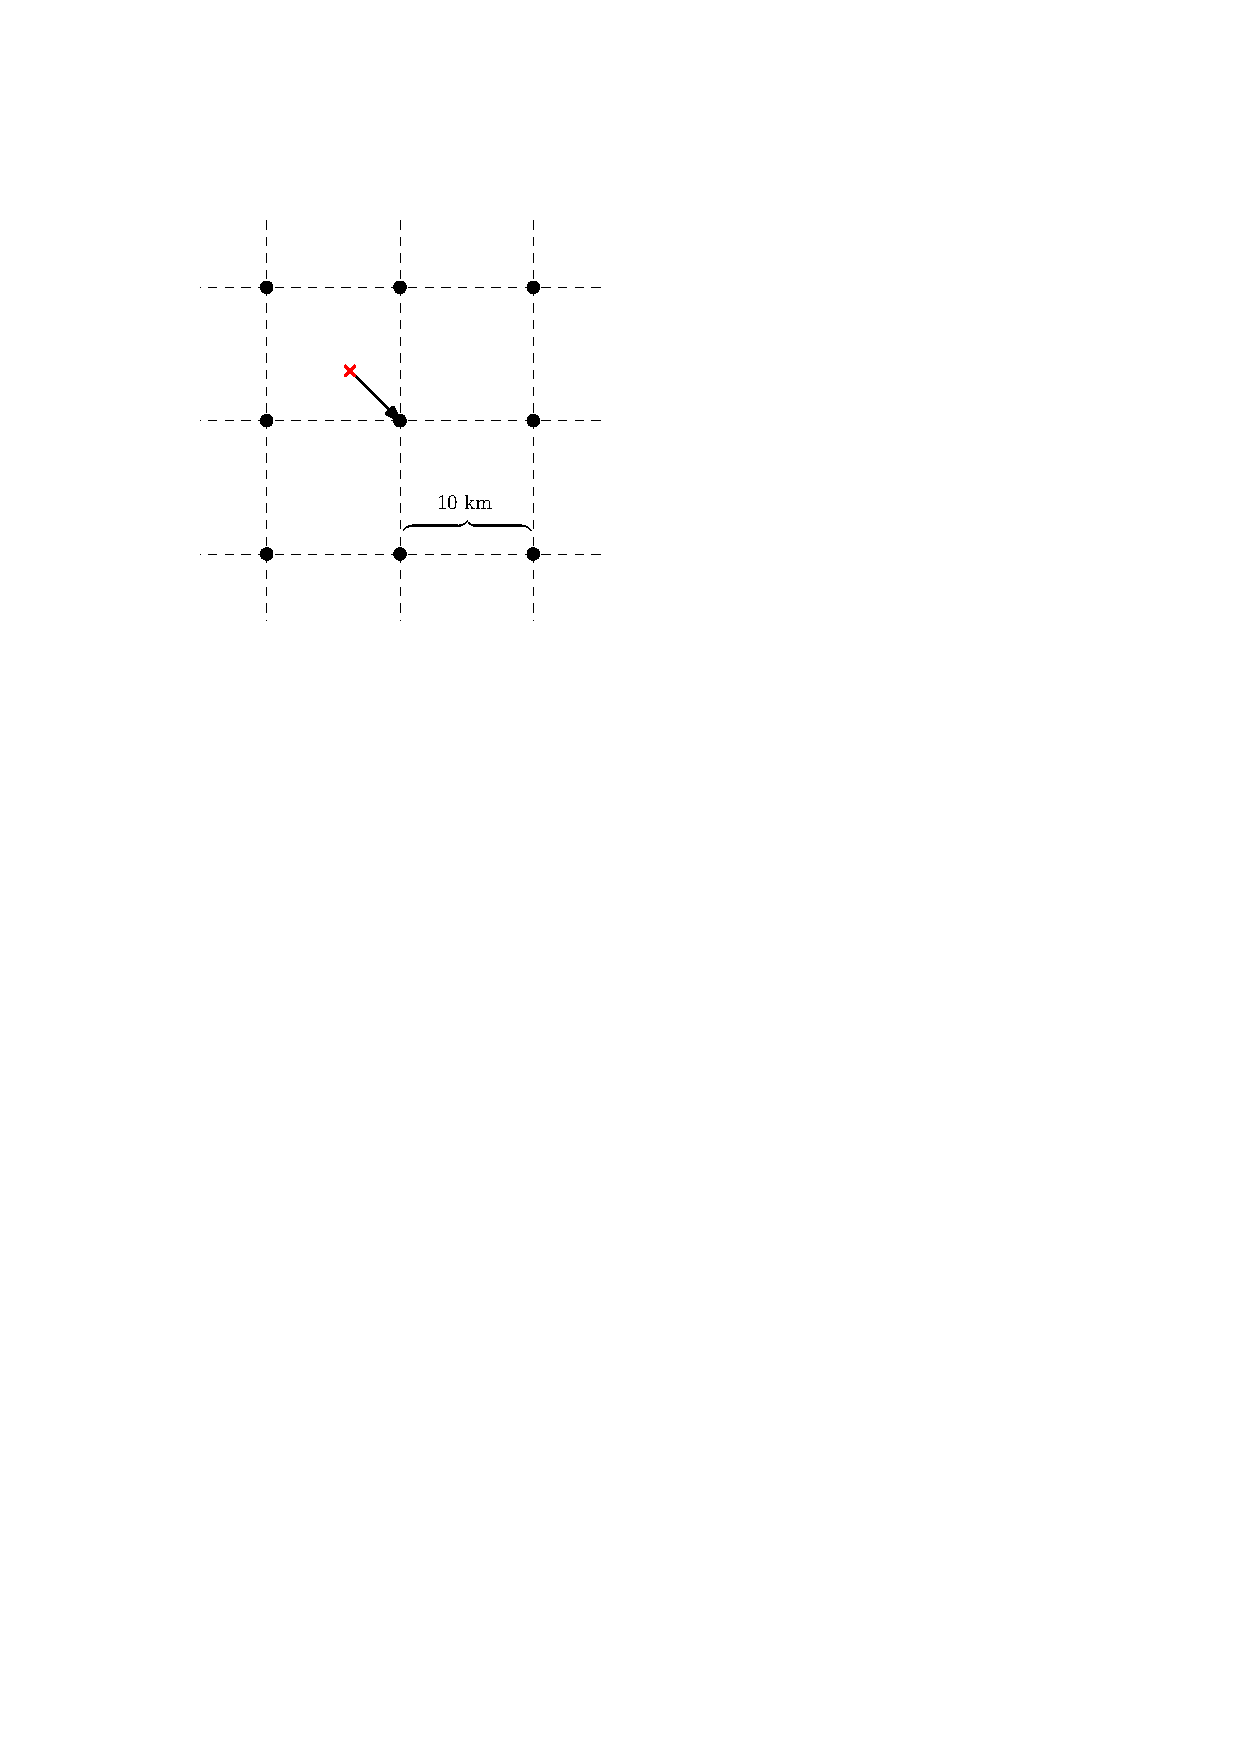
\includegraphics[width=.4\columnwidth]{location_privacy/location_grid_truncation_example}
  \caption{The user (represented by the red cross) has their location
    truncated to a grid of fixed points.}
  \label{fig:grid-truncation-example}
\end{figure}

Once we can intercept calls that pass location information to the app,
it is easy to modify the coordinates however we wish. For our
experiments, we truncate location information, snapping to a
user-specified grid, as illustrated in
Figure~\ref{fig:grid-truncation-example}.  Formally, our
implementation truncates to a grid with spacing $s$ in kilometers
using the formulae:

\begin{displaymath}
  \begin{array}{cc}
%    s_\textit{lat} = s \cdot \Delta^{\textit{lat}} &
    \textit{lat}' = s_\textit{lat} \lceil \textit{lat} /s_\textit{lat} \rceil &
%    s_\textit{long} = s \cdot \Delta^{\textit{long}} &
    \textit{long}' = s_\textit{long} \lceil \textit{long} /s_\textit{long} \rceil
  \end{array}
\end{displaymath}

\noindent where \textit{lat} and \textit{long} are the actual latitude and
longitude, and their primed versions are the new coordinates. Here
$s_\textit{lat}$ and $s_\textit{long}$ are the grid spacing translated
into degrees of latitude and longitude, respectively.
%$\Delta^{loc}$ is number of degrees per meter, which differs for latitude and
%longitude.  
For latitude we use the WGS 84 approximation for North America \cite{latitude-calculator}:

\begin{displaymath}
s_\textit{lat} = \frac{s~\textrm{km}}{111.5~\textrm{km/deg}}
\end{displaymath}

For longitude we use a standard approximation \cite{rapp:geometric}:

\[
s_\textit{long} = s~\textrm{km} \cdot 
  \frac {180 \sqrt{(1 - e^2 \sin^2(\phi))}}
  {\pi a \cos(\phi)}
\]

\noindent where $e^2 = (a^2 - b^2)/b^2$ is the eccentricity of Earth, $\phi$ is
the latitude, $a$ is the radius to the
equator, and $b$ is the radius to the poles.

We verified that \fuzzer{} works correctly in two ways.  First, we 
inserted logging code in \fuzzer{} to give the original position and 
position after location truncation.  We then took the set of locations from our 
testcases, truncated them to varying amounts, and then verified the
resulting positions were correct.  Second, we confirmed that our subject apps'
behaviors changed in sensible ways as we varied the location truncation 
amount.

The Android location manager API also can provide speed information,
which our implementation truncates speed using a similar
formula. However, none of our subject apps use speed
information. Moreover, device-reported speed is often unreliable, so
many apps ignore it, preferring instead to estimate speed using
successive location fixes.

\subsection{Experimental Design}
\label{sec:design}

\begin{figure}
  \small
  %% XXX
  \begin{subfigure}[t]{\columnwidth}
    \centering
    \begin{tabular}{|l|l|}
      \hline
      Name & Objects in List \\ \hline \hline
      \gasbuddy & Gas stations \\
      \restaurantfinder & Restaurants \\
      \hospitals & Hospitals \\
      \webmd & Pharmacies and clinics \\
      \walmart & Stores \\
      \tdbank & ATMs and branches \\
      \hline
    \end{tabular}
    \caption{Descriptions of each subject app.}
    \label{fig:app-descriptions}
  \end{subfigure}

  \bigskip{}

  \begin{subfigure}[t]{\columnwidth}
      \centering
      \begin{tabular}{|l|r|r|}
        \hline
        City & Population & Radius (km) \\ \hline \hline
        New York, NY & 8,200,000 & 30 \\ \hline
        Dallas, TX & 1,200,000 & 20 \\ \hline
        New Haven, CT & 130,000 & 10 \\ \hline
        Baltimore, MD & 620,000 & 12 \\ \hline
        Redmond, WA & 54,000 & 4 \\ \hline
        Decatur, TX & 6,000 & 4 \\ \hline
      \end{tabular}
      \caption{Selected population centers.}
      \label{fig:regions}
    \end{subfigure}

    \bigskip{}

    \begin{subfigure}[t]{\columnwidth}
      \centering
      \begin{tabular}{|r|r|r|r|r|} \hline
        0 km & 0.1 km & 0.2 km & 0.5 km & 1 km \\ \hline
         2 km & 5 km & 10 km & 20 km & 50 km \\ \hline
      \end{tabular}
      \caption{Truncation amounts tested.}
      \label{fig:truncations}
    \end{subfigure}

  \caption{Experimental parameters.}
\end{figure}
 
We conducted a systematic study of the effect of location truncation
on apps that list nearby objects, the largest category in
Figure~\ref{fig:location-uses} for which location truncation's effect is clearly
measurable. We selected a variety of such apps, listed in
Figure~\ref{fig:app-descriptions}, from Google Play. We chose apps
that rely on a variety of different data sets and run under our tool
chain with minimal difficulty.
We then modified each app using \fuzzer, as outlined
in Section~\ref{sec:impl}. Next, we randomly chose a set of locations and
then captured the output list of each app as we varied the current
location and the amount of truncation applied to it. Finally, we used
several metrics to estimate how each truncation affected the app's
utility.

\subsubsection{Locations and truncations}

In a pilot study, in which we examined the results of \fuzzer{} on a
variety of apps, locations, and truncations in an ad hoc manner,
we noticed that truncation has quite different
effects depending on where apps are
run. For example, there is a significantly higher density of restaurants in
a big city than in a rural area, causing one of our subject apps,
Restaurant Finder, to behave very differently under truncation in each locale.
Thus, in selecting locations for
our study, we chose them from a range of population centers of varying
sizes, as shown in Figure~\ref{fig:regions}. 

We modeled each city as a circle centered on the geographical 
city center with a radius estimated
from looking at a map of the region. In
our pilot study, we also found that many apps produce error screens if
given a location that cannot be mapped to a real address, e.g., if the
current location is in the ocean or a heavily forested area.
Thus, we discarded any random points that caused 
problematic outputs from our apps, and randomly picked new
points until we had a set of 10 points that produced correct output
across all apps when the apps were run with no truncation.

For each random location, we ran each app with 10 different truncation
amounts (including no truncation), listed in
Figure~\ref{fig:truncations}.  We chose an upper limit of 50 km because 
many of our subject apps
give results up to or less than 50 km, so the metrics would
be undefined beyond that level.

\subsection{Metrics used for evaluation}
\label{sec:metrics}

Recall from Section~\ref{sec:usage} that we identified apps that list
nearby objects as the best candidate for our study of location
truncation. For example, Figure~\ref{fig:app-example} gives two
screenshots of the Restaurant Finder app being run on a location in
New York, NY (close to Bloomfield, NJ) both without and with
truncation. Here the lists we consider are the restaurants, in order
from closest to farthest, along with their distances.

We explored three ways to measure location truncation's effect on
the output list of such apps: edit distance of the changed list from the
original, the size of the intersection of the original and changed
lists, and the additional distance of the first (closest) list item on
the changed list.

\begin{figure}
  \centering
  \begin{tabular}{cc}
    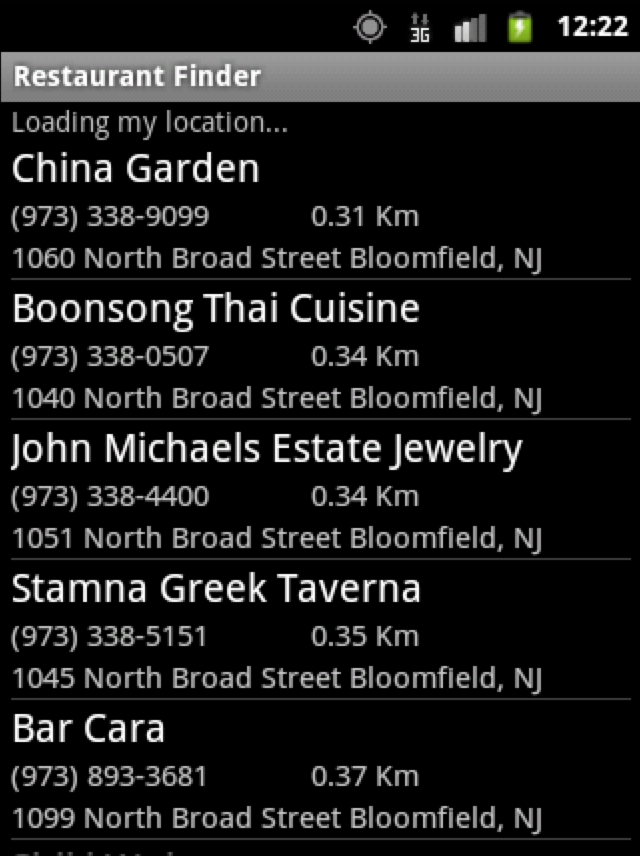
\includegraphics[width=.4\columnwidth]{location_privacy/restaurant_finder_ref_screenshot}
    & 
    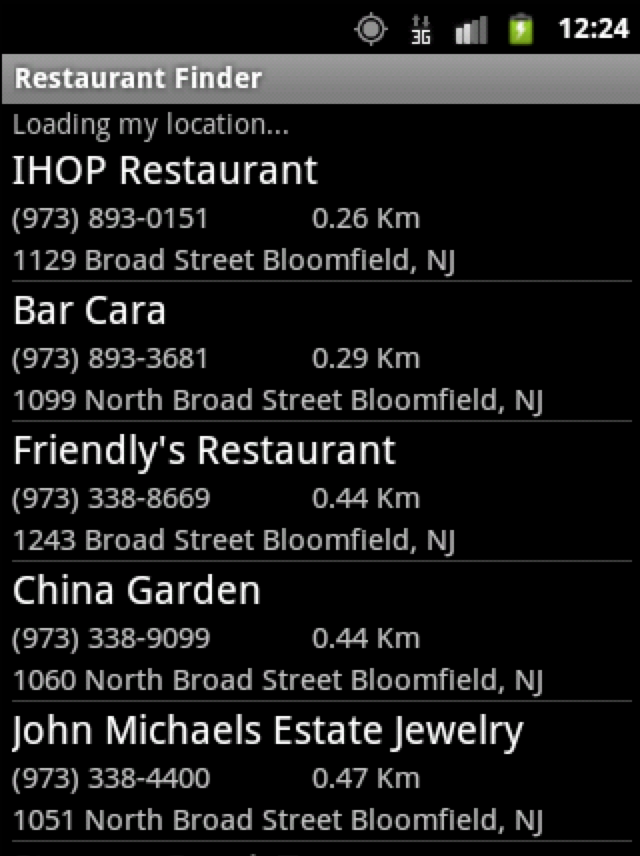
\includegraphics[width=.4\columnwidth]{location_privacy/restaurant_finder_nominal_screenshot}
  \end{tabular}
  \caption{Restaurant Finder without (left) and with (right)
    0.2~km of truncation.}
  \label{fig:app-example}
\end{figure}

\subsubsection{Edit distance}

The first metric we investigated is \emph{edit distance}, which is the
number of edits (insertions, deletions, or swaps) needed to change one
list into another~\cite{levenshtein:1966}. For
example, the edit distance between the lists in
Figure~\ref{fig:app-example} is five, because every item in the
list has changed.

Like the other apps we studied, Restaurant Finder returns more than
one screenful of objects. Thus, in performing our measurements, we
need to decide how much of the app's output to use. We could pick only
the first screen of data, but this restricts edit distance to just
a few possible values. We could pick all the results, but that has the
disadvantage that there could be many changes in the long tail of a
list, yet few users would bother looking that far. Thus, as a
compromise, we opted to compute edit distance over the first four
screens of an app, which we think covers typical usage patterns while
providing useful data.  In each of the apps we tested, this corresponded 
to the first twenty list elements.

\subsubsection{Set intersection size}

Edit distance was the first metric we thought of, but when we tried
measuring it, we found it to be
problematic: Especially on the first screen of data, many locations
are very close, e.g., on the left of
Figure~\ref{fig:app-example}, distances range from 0.31~km to
0.37~km. Yet edit distance would count reorderings of those locations
in the metric.

Thus, we also explored using set intersection size as a metric. We
ignore ordering and compute how many objects are in both the original
and changed list. For example, in Figure~\ref{fig:app-example}, the set
intersection has size three. As with edit distance, we compute the
intersection on the list displayed across the first four screens of
output.

The set intersection metric is also more natural than edit distance in
that it corresponds directly to a common user task of checking whether
some particular object is nearby. For example, we might use Restaurant Finder
to ask, is there any McDonalds nearby, or we might use GasBuddy to
look for the closest Shell station.

\subsubsection{Additional distance incurred}

Ideally, we would like to measure how actual users' behavior is
affected by location truncation, but this is difficult to do without a large
number of human participants. Instead, we developed an \emph{additional
  distance} metric that computes how much farther a user who always
picks the first list item would go given the changed list compared to
the original list.

For example, in Figure~\ref{fig:app-example}, the closest restaurant
is actually China Garden, 0.31 km away. However, under truncation, the
closest restaurant appears to be an IHOP. While the IHOP's reported
distance is 0.26 km, that is the result from the truncated
location---we need to look at the original output list to find out how
far away the restaurant actually is. In this case, IHOP appears on the
second screen of the original list, and it is 0.42~km
away. For this example, then, the additional distance is $0.42 - 0.31
= 0.11$~km.

Restating this more generally, let $D(X)$ be the distance to object
$X$ on the original list. Then the additional distance of a changed
list is $\Delta = D(\textit{First original}) - D(\textit{First changed})$, where
\textit{First original} is the first item of the original list and
\textit{First changed} is the first item of the changed list. Notice
that this metric may be undefined if \emph{First changed} does not
appear on the original list. To reduce the chances of this, we
consider all output screens of an app in computing the metric, and not
just the first four screens. However, in our experiments the metric is
still sometimes undefined for some apps under large truncation amounts.

\subsubsection{Testing infrastructure}

To compute the results of our experiments, we needed to run each
subject app at 60 locations and 10 different truncation
amounts. This is clearly far too many configurations to run by
hand. Instead, we developed testing infrastructure to let us run each
configuration automatically, scrape the resulting output lists, and
then run our metrics on the result.

The core technology we used is Troyd \cite{jsjeon:troyd}, an open
source, black box testing framework that can execute apps (e.g.,
launch them, click buttons, enter text boxes, scroll the screen, etc.)
and gather text from the GUI.  Troyd allows us to write a high level
test case (e.g., to click a sequence of buttons and gather some text)
that can be reused for various test configurations.  We developed a
server that takes an app modified by \fuzzer{}; resigns it with a
shared user ID so that it can be controlled by instrumentation; and
then runs testcases against the app using Troyd.

We ran apps on both Google Nexus S devices and on device emulators;
our infrastructure works the same in both cases, and performing some
runs on actual devices acted as a sanity check. In all cases, the
Android platform was Gingerbread 2.3.3 with the Google APIs, such as
maps, installed. These APIs are special dynamic libraries licensed by
Google and not included on plain Android distributions; these APIs are
needed for the subject programs to run.

We found that, while Troyd mostly did what we wanted, we needed to
extend it to handle additional GUI elements.
For example, while Troyd can capture the currently visible GUI elements,
many \code{Views} (such as those in \code{ListView} elements) are 
reused, and their contents only appear when the screen is scrolled.
Thus, we extended Troyd with special functionality to 
navigate to screens that may have unrendered information.
We also found that, as is usual in large-scale
testing, 
experimental tests sometimes failed unpredictably, e.g., an emulator
or device would crash for no apparent reason. These are likely due to
subtle bugs lurking in the OS or emulator implementation that
were tickled by the experiment's atypical usage pattern. Thus, our
testing infrastructure catches any failed runs and reschedules those
experiments to be run again. Finally, our testing infrastructure allows
multiple experiments to be done in parallel; the majority of the
experiments were done on a machine with six Intel Xeon processors, 
each with four cores, and 48 GB of RAM.  Each individual test took on
the order of a few minutes to run, depending on the app.
Our tests ran up to fifteen emulators at once.

\begin{figure*}[t!]
  \centering
  \begin{tabular}{ccc}
    
    \begin{minipage}{2in}
      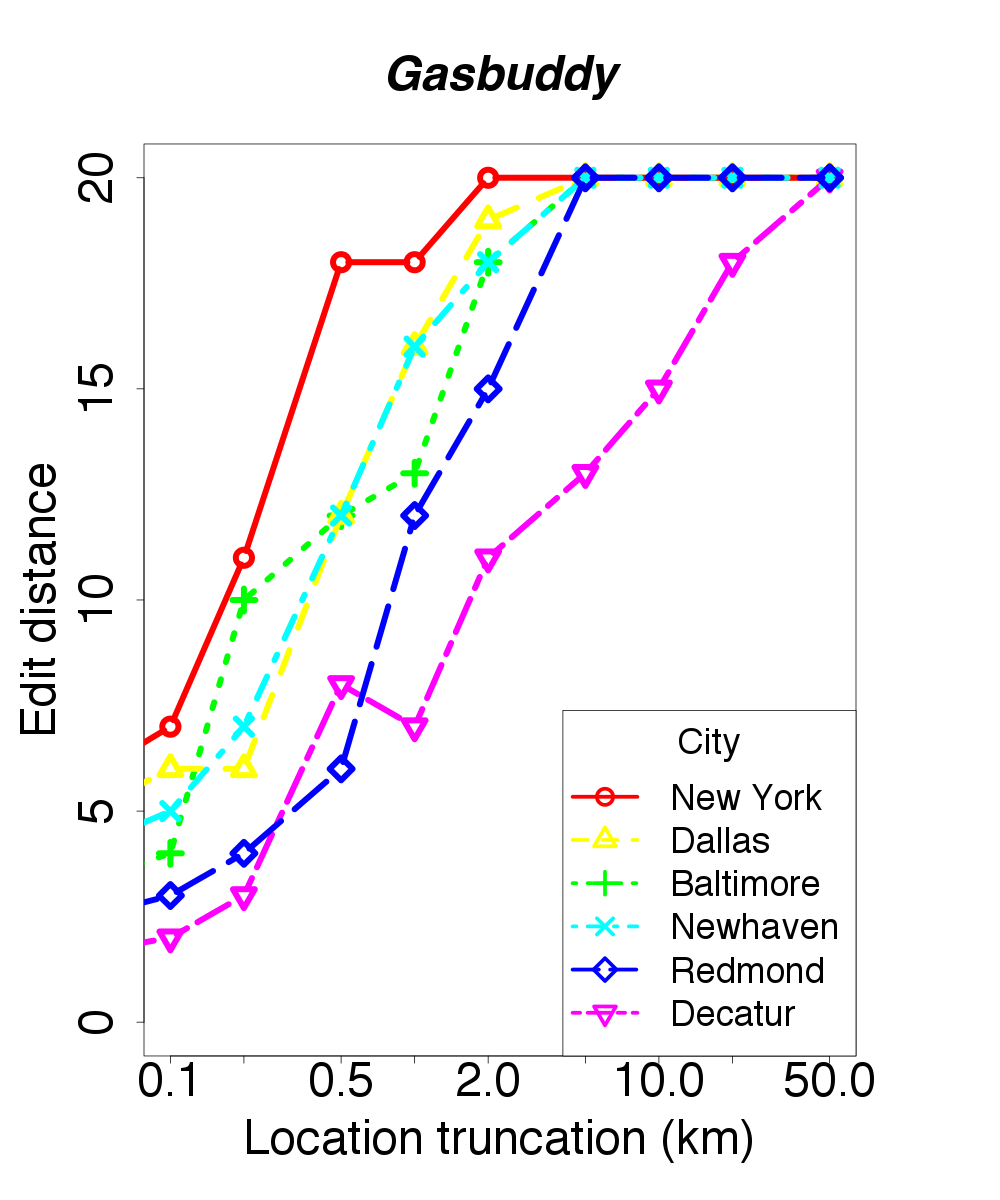
\includegraphics[width=\textwidth]
                      {location_privacy/data/gasbuddy/plots/medians_across_city_20}
    \end{minipage}
    
    % [width=.6\textwidth]
    \begin{minipage}{2in}
      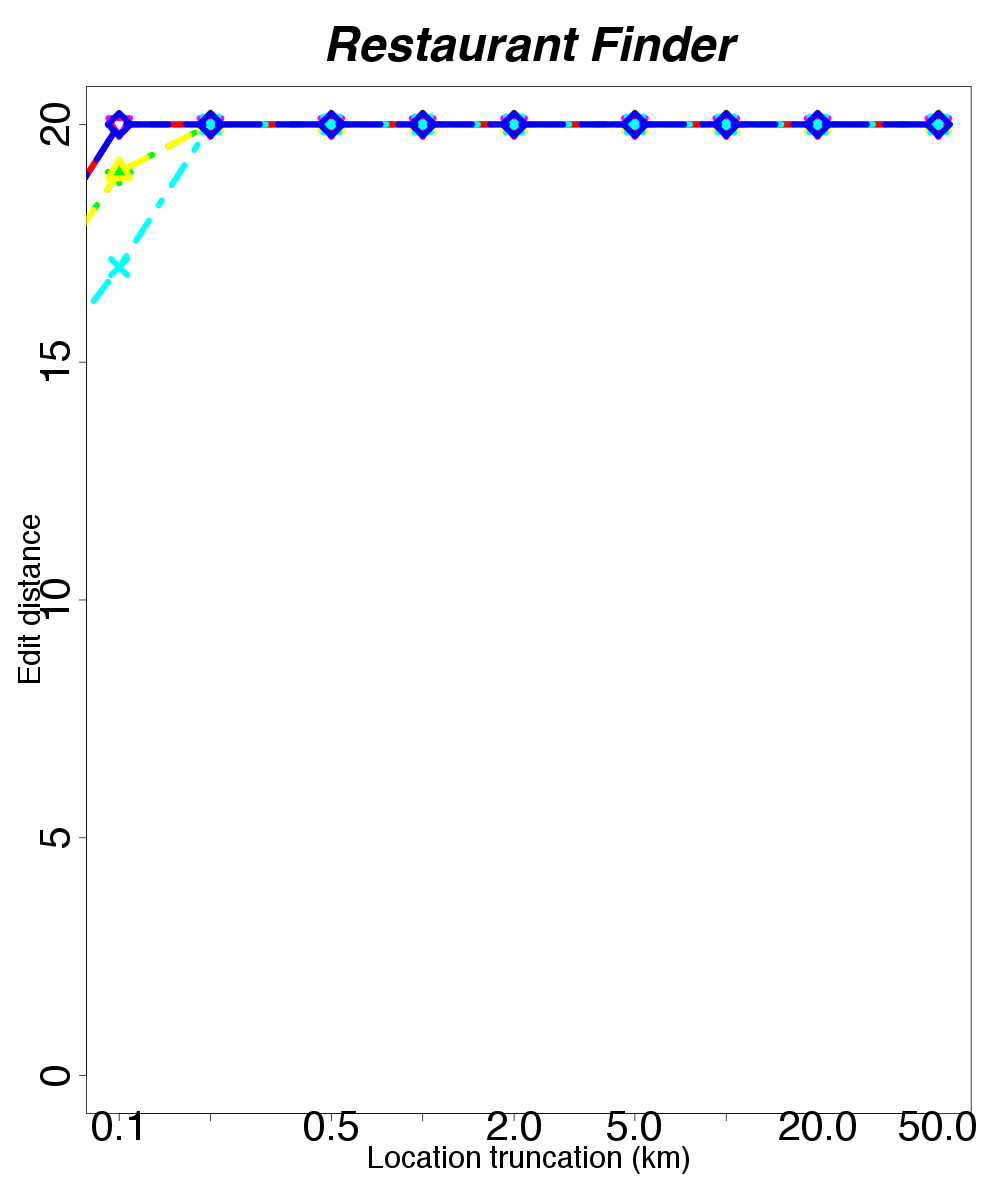
\includegraphics[width=\textwidth]
                      {location_privacy/data/restaurant_finder/plots/medians_across_city_20}
    \end{minipage}
    
    \begin{minipage}{2in}
      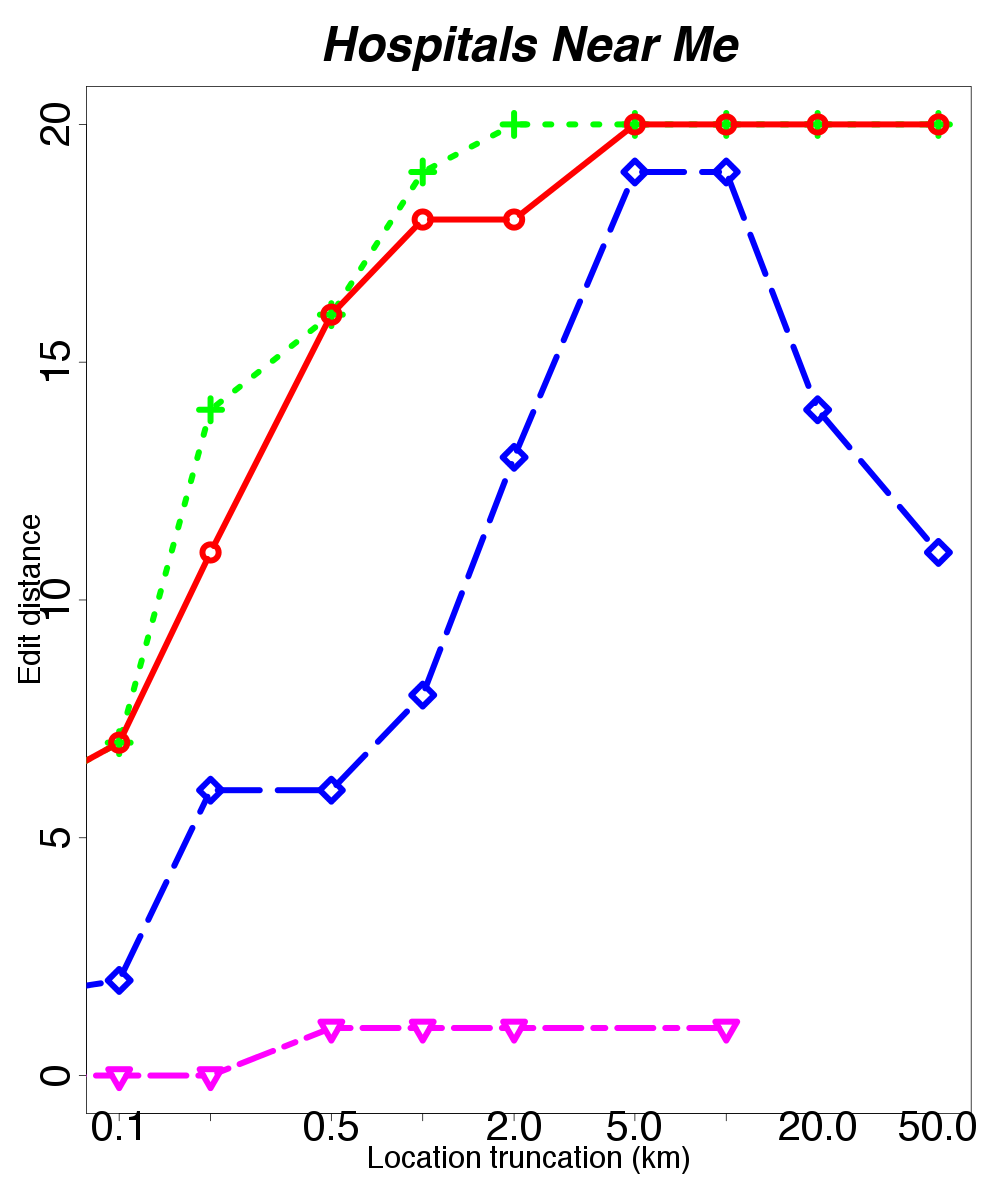
\includegraphics[width=\textwidth]
                      {location_privacy/data/hospitals/plots/medians_across_city_20}
    \end{minipage}
    
    \\
    \begin{minipage}{2in}
      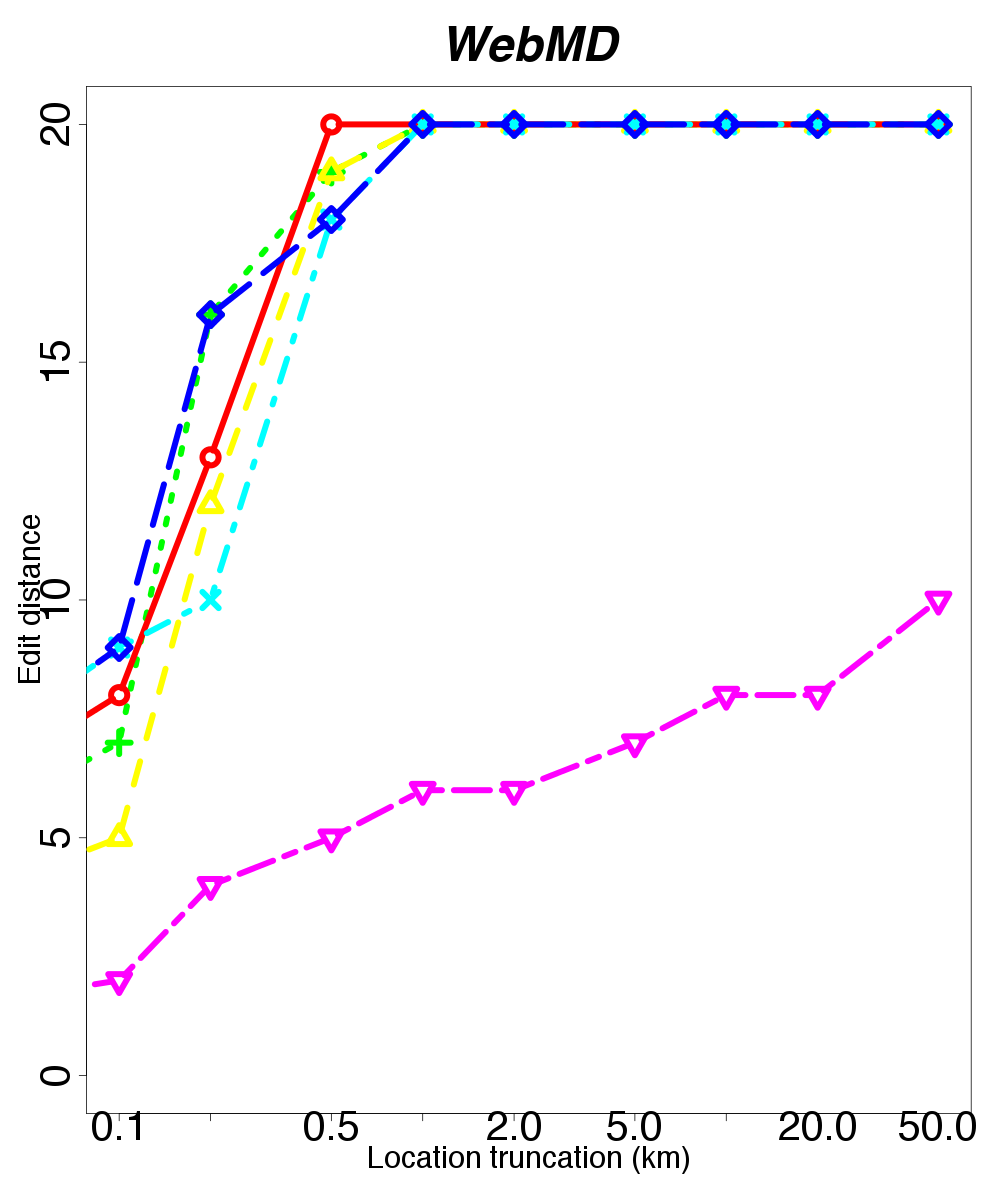
\includegraphics[width=\textwidth]
                      {location_privacy/data/webmd/plots/medians_across_city_20}
    \end{minipage}
    
    \begin{minipage}{2in}
      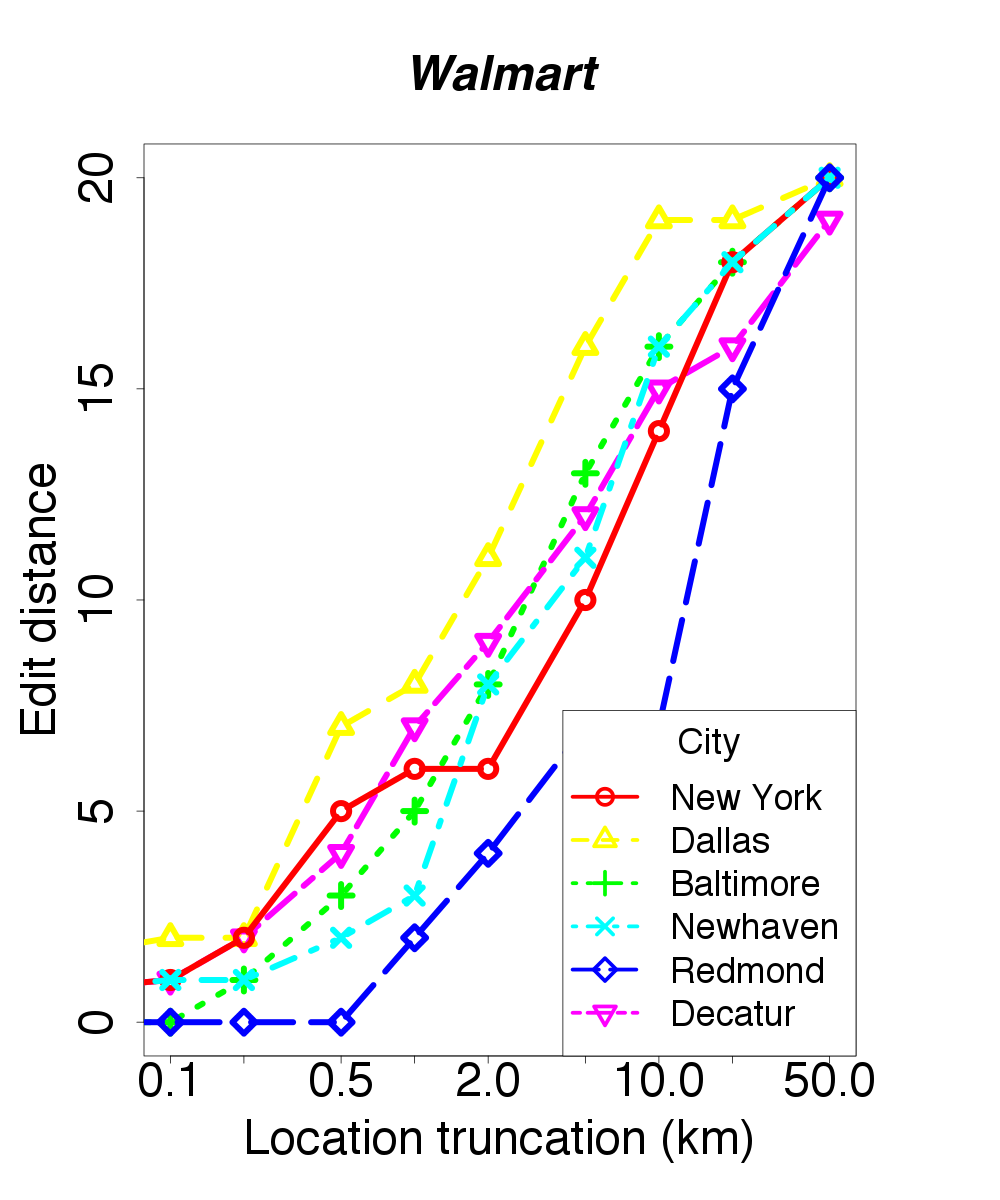
\includegraphics[width=\textwidth]
                      {location_privacy/data/walmart/plots/medians_across_city_20}
    \end{minipage}
    
    \begin{minipage}{2in}
      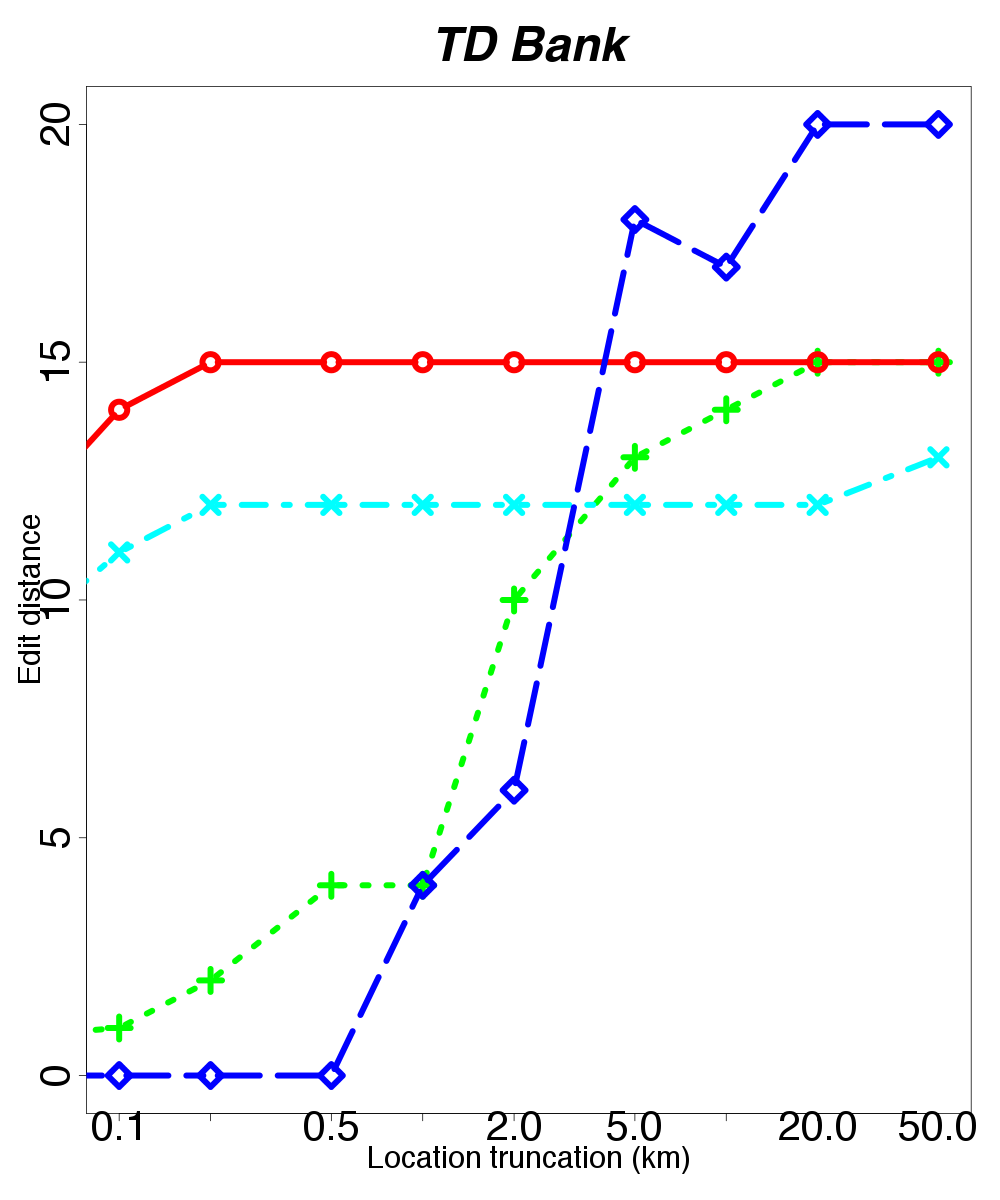
\includegraphics[width=\textwidth]
                      {location_privacy/data/tdbank/plots/medians_across_city_20}
    \end{minipage}
  \end{tabular}
  \caption{Graphs of median edit distance versus truncation
    amount. Higher edit distance implies lower utility.}
  \label{fig:edit-distance-metric}
\end{figure*}

\subsection{Results}
\label{sec:results}

Finally, we present the results of our study. At a high level, we
found that across our
subject apps and locations, location can be
significantly truncated without significantly harming utility: up to 20~km
when an app is used in a lower population area, and usually (for five of six apps) 
at least 5~km in more populous areas.  We also found that apps have relatively little 
change in utility up to a certain amount of truncation, typically
about 5~km, after 
which the app's output becomes much less usable.  Finally, we found that the factor 
that most determines the ability to truncate location was the density
of the set of locations the app computes over.

In the discussion that follows, we include several plots. In each
plot, the $x$-axis is the truncation amount; note that because of our
choice of truncations, this axis is essentially log-scale.  The $y$-axis
is the median of one of our metrics on the 10 randomly chosen points
for each population center.

We next consider each of our three metrics in turn.

\begin{figure*}[t!]
  \centering

  \begin{subfigure}[t]{\textwidth} 
    \begin{tabular}{ccc}
    
    \begin{minipage}{2in}
      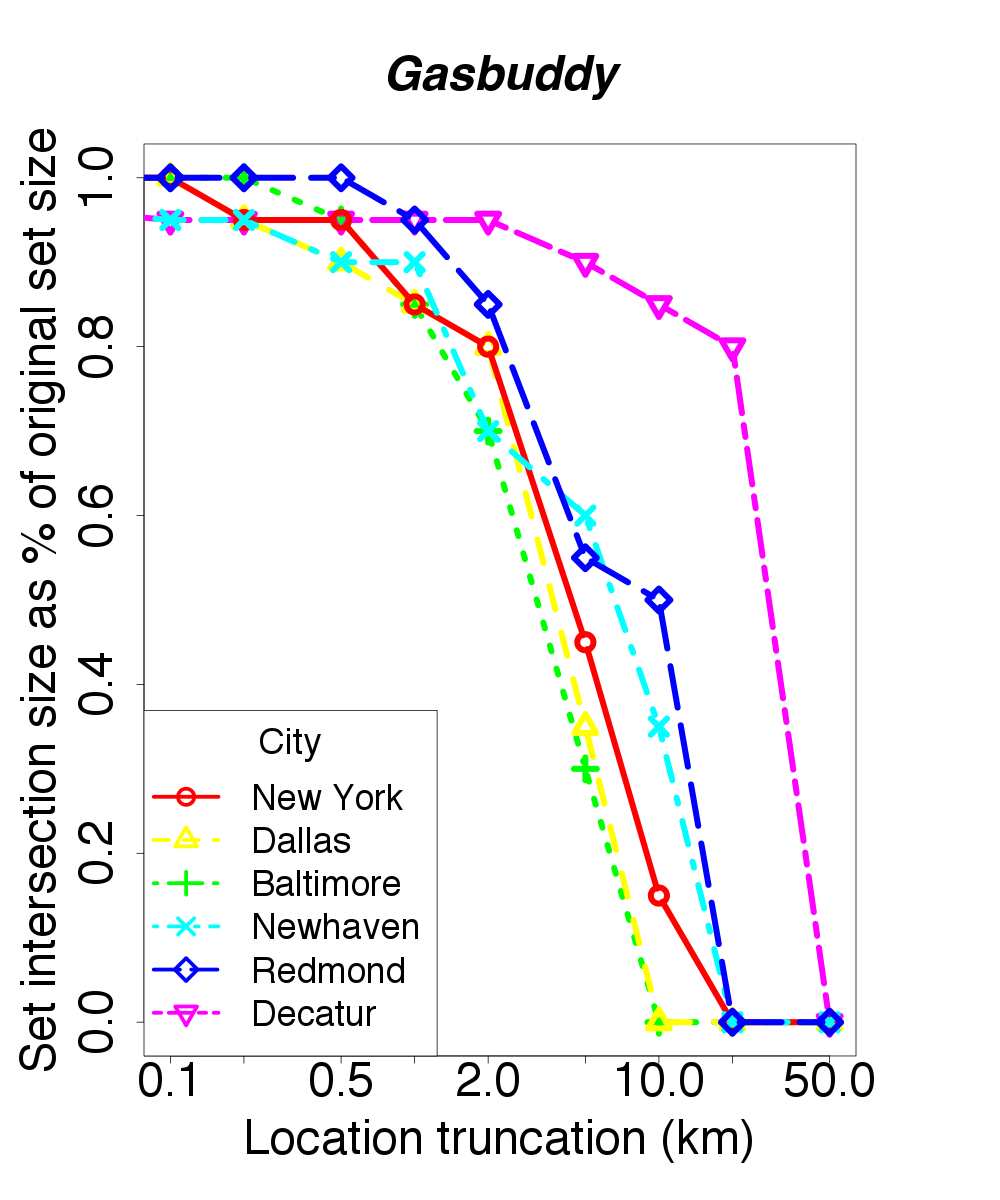
\includegraphics[width=\textwidth]
                      {location_privacy/data/gasbuddy/plots/medians_across_city_si_20}
    \end{minipage}
    
    % [width=.6\textwidth]
    \begin{minipage}{2in}
      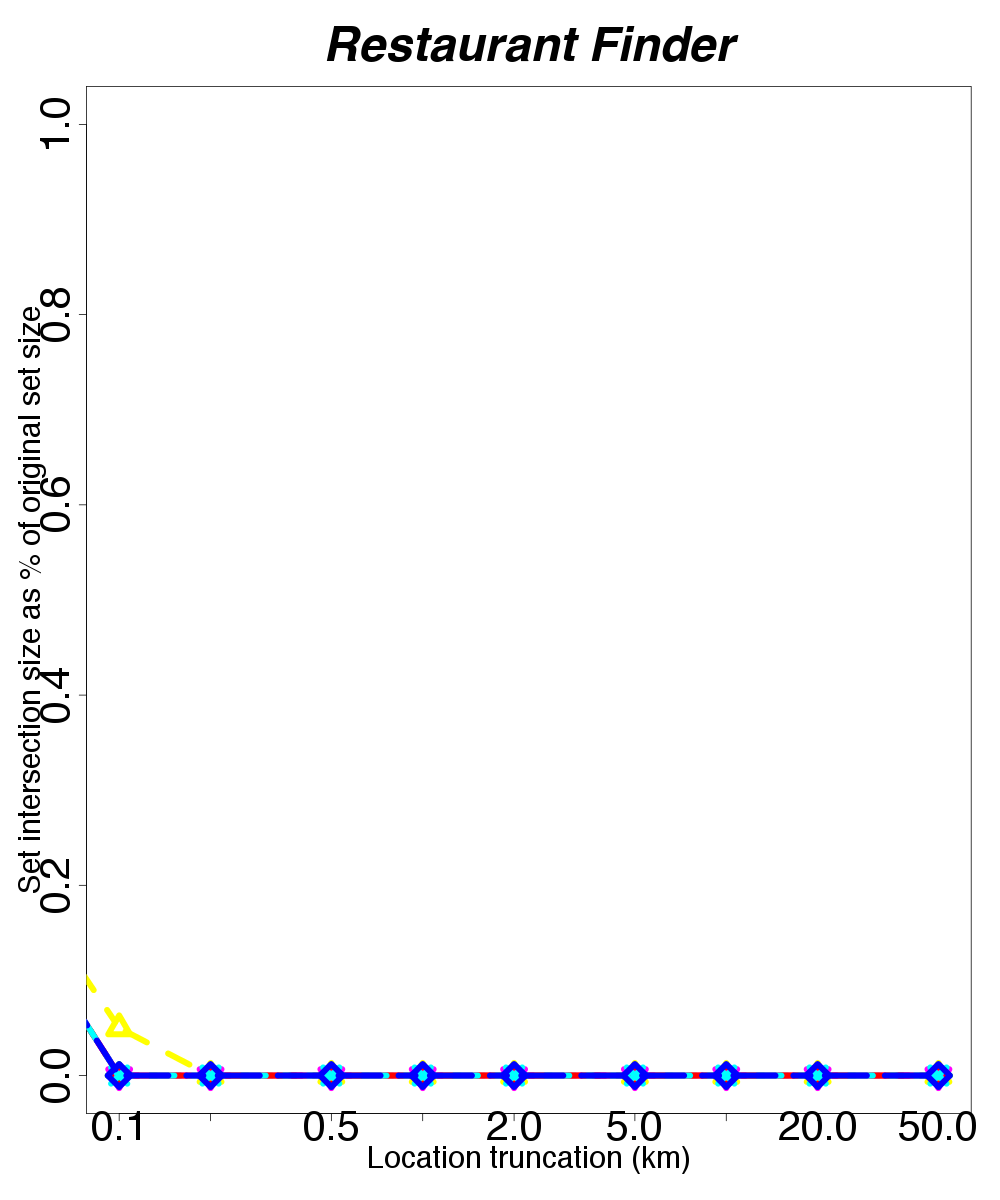
\includegraphics[width=\textwidth]
                      {location_privacy/data/restaurant_finder/plots/medians_across_city_si_20}
    \end{minipage}
    
    \begin{minipage}{2in}
      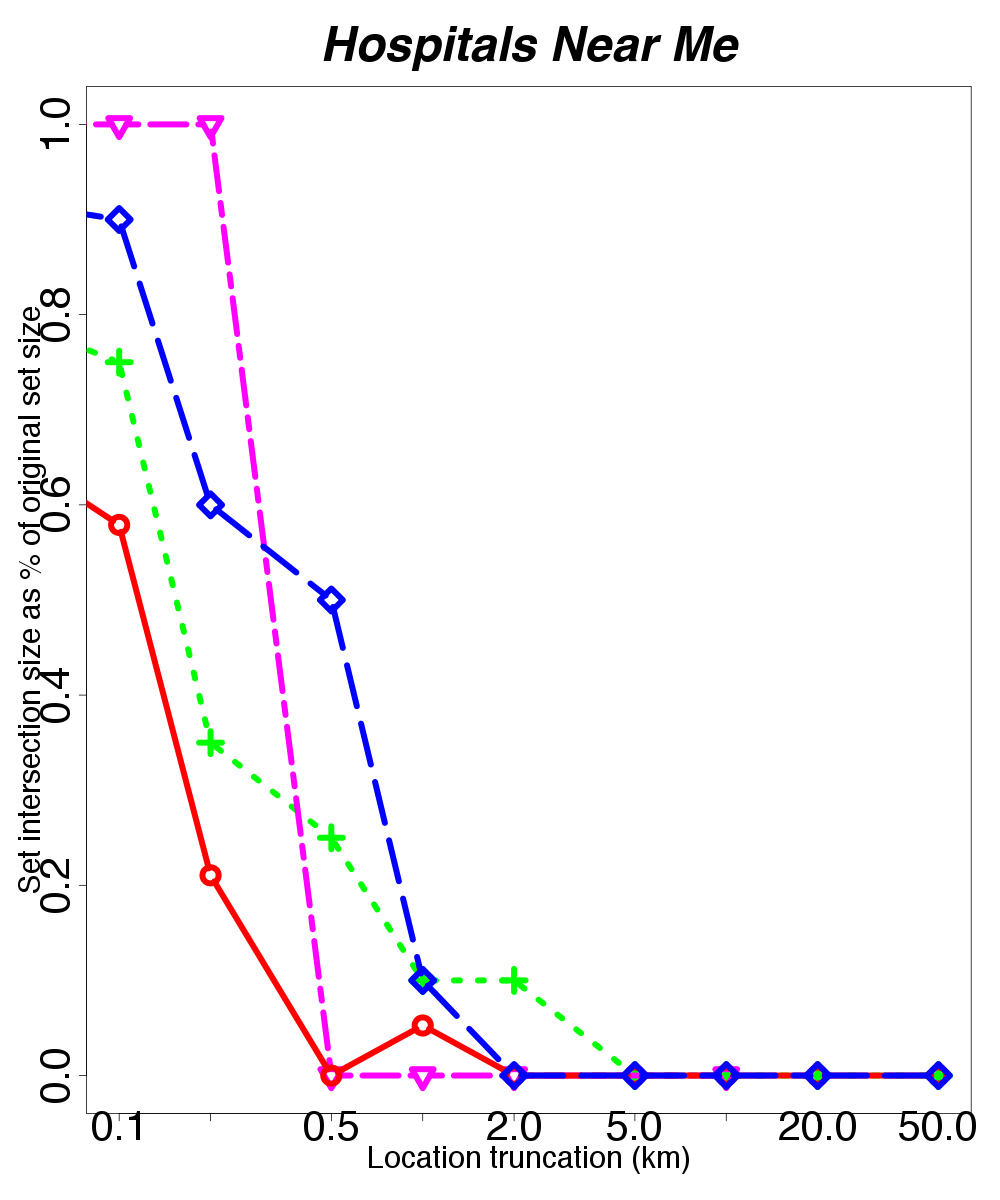
\includegraphics[width=\textwidth]
                      {location_privacy/data/hospitals/plots/medians_across_city_si_20}
    \end{minipage}
    
    \\
    \begin{minipage}{2in}
      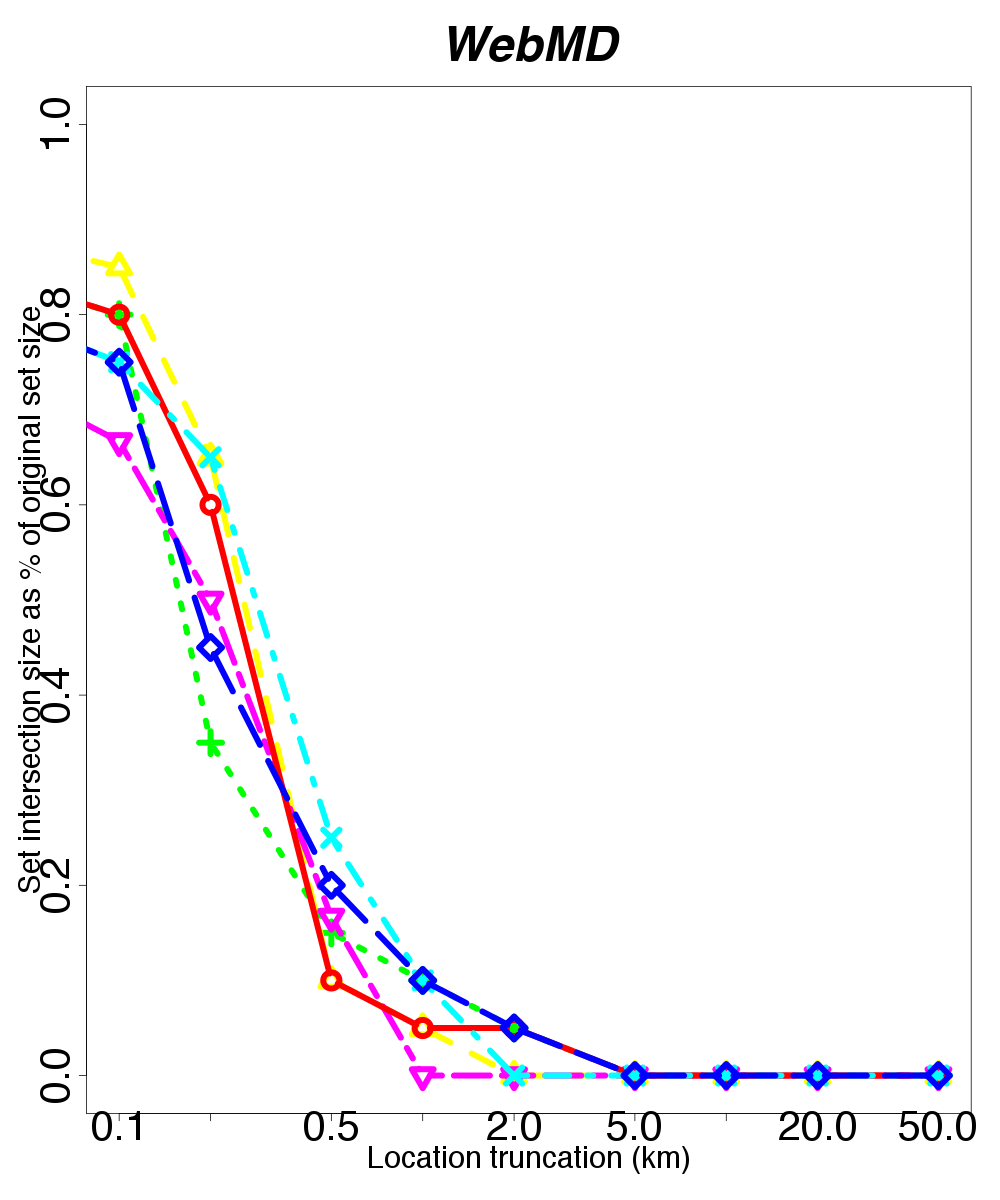
\includegraphics[width=\textwidth]
                      {location_privacy/data/webmd/plots/medians_across_city_si_20}
    \end{minipage}
    
    \begin{minipage}{2in}
      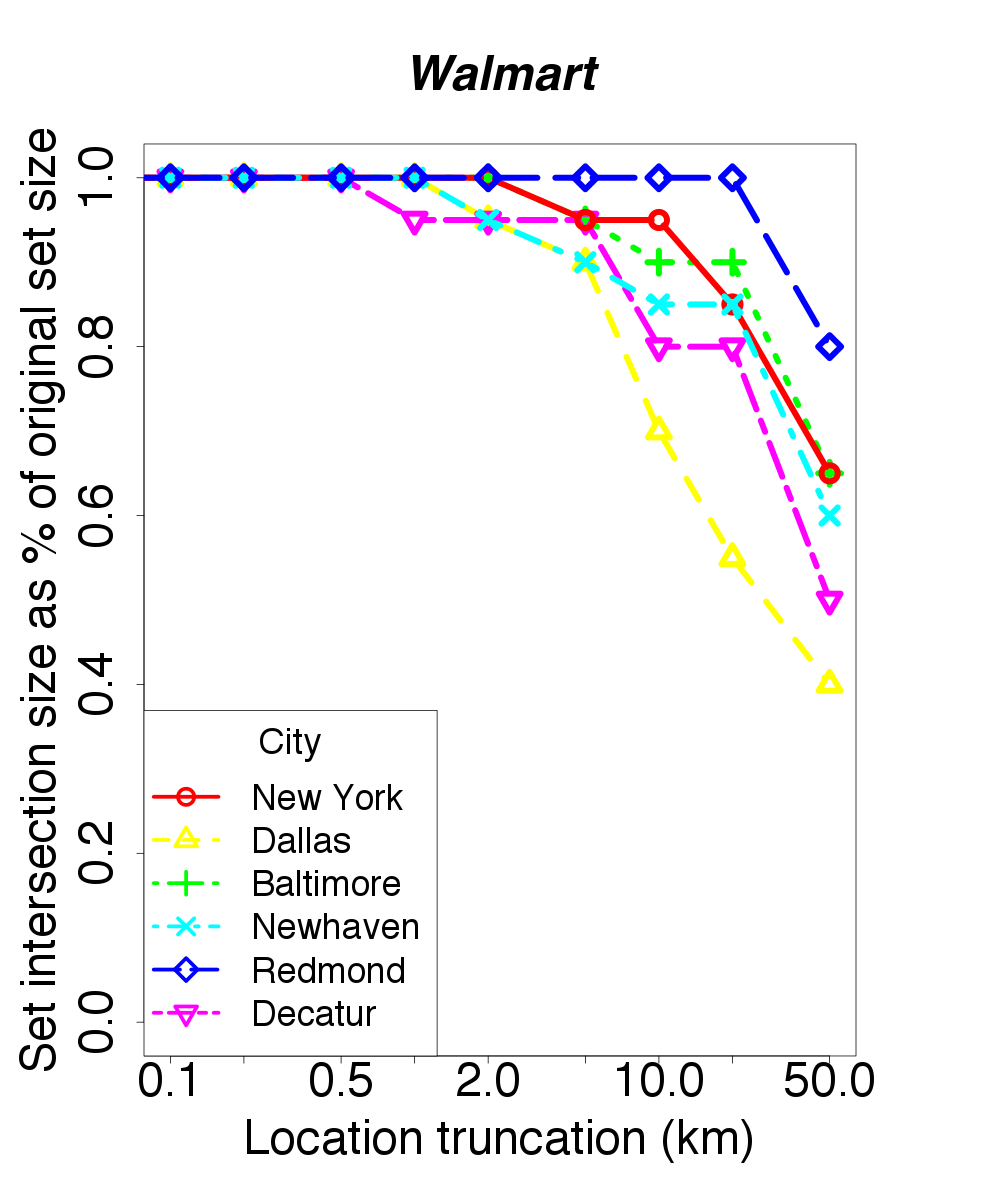
\includegraphics[width=\textwidth]
                      {location_privacy/data/walmart/plots/medians_across_city_si_20}
    \end{minipage}
    
    \begin{minipage}{2in}
      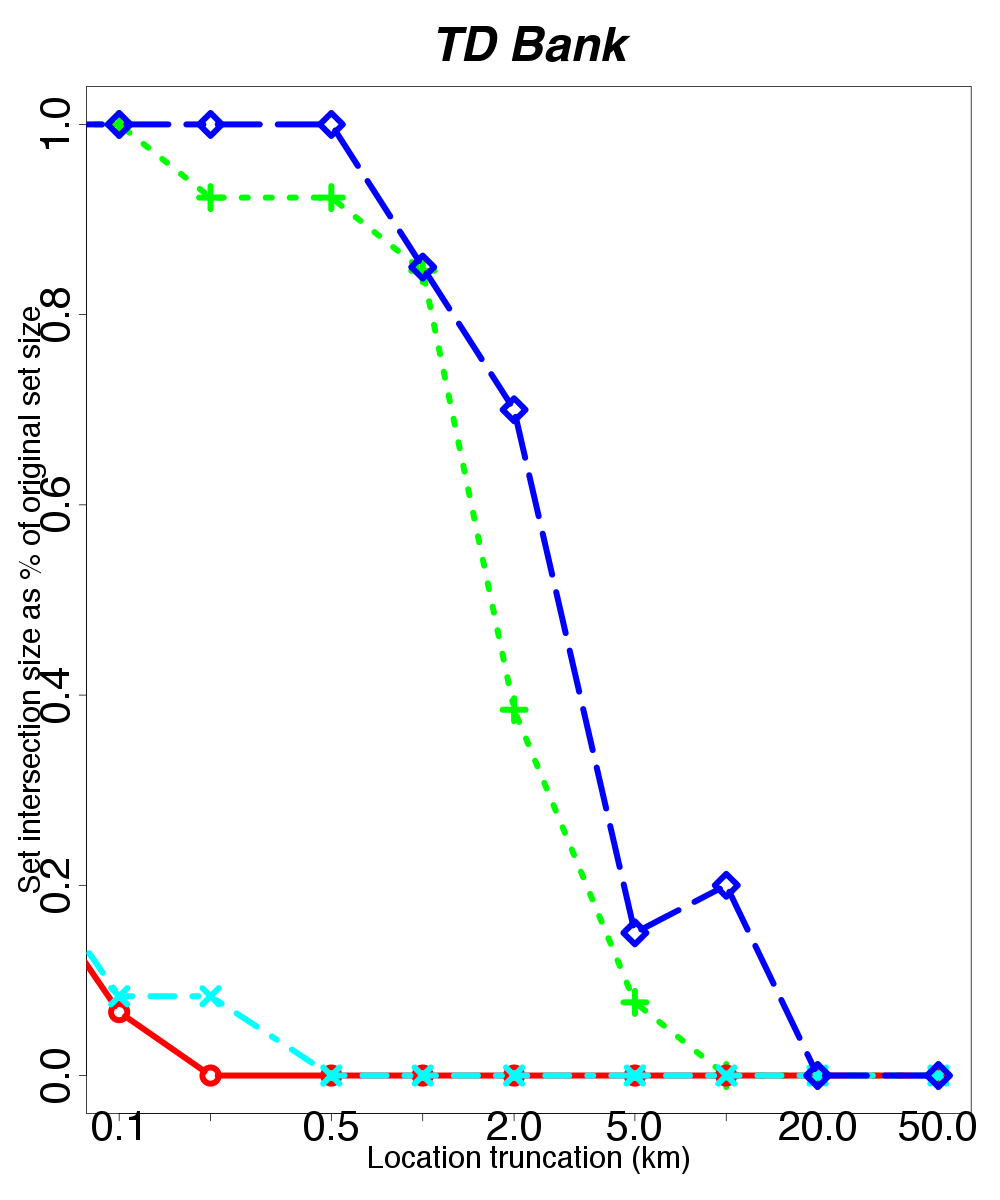
\includegraphics[width=\textwidth]
                      {location_privacy/data/tdbank/plots/medians_across_city_si_20}
    \end{minipage}
  \end{tabular}
  \caption{Graphs of median set intersection size versus
    truncation amount. Lower set intersection size indicates lower
    utility.}
  \label{fig:set-intersection-metric}
  \end{subfigure}

  \bigskip{}

  \begin{subfigure}[t]{\textwidth}
 \small
 \centering
 \begin{tabular}{|l|rrrrrr|}
 \hline
 & New York & Dallas & Baltimore & New Haven & Redmond & Decatur \\
 \hline
 Gasbuddy & 5 & 5 & 2 & 2 & 5 & 50 \\
Restaurant Finder & 1 & 0.5 & 0.1 & 0.1 & 0.1 & 0.2 \\
Walmart & 50 & 10 & 50 & 50 & $\cdot$ & 50 \\
TD Bank & 10 & $\cdot$ & 50 & 20 & $\cdot$ & $\cdot$ \\
WebMD & 10 & 5 & 2 & 10 & 10 & 50 \\
Hospitals Near Me & 5 & $\cdot$ & 20 & $\cdot$ & 20 & $\cdot$ \\
\hline

\end{tabular}
 \caption{Largest truncation amount (km) before which the median set
   intersection size is lower than 80\%.}
 \label{fig:knee-points-set-cutoff}
  \end{subfigure}
  
  \caption{Set intersection size results.}
\end{figure*}

\subsubsection{Edit Distance}

Figure~\ref{fig:edit-distance-metric} shows how edit distance 
 varies
on our location set.  
Note that Hospitals Near Me and TD Bank do
not have data for cities for which the app did not generate enough output
to calculate a significant result. 
For example, there are no TD banks in Dallas.  In some cases,
TD Bank and Hospitals Near Me do generate data, but they generate 
a very small set of results (Hospitals Near Me only returns hospitals
within 50 miles, for example).
Thus, edit distance appears to go down
at large truncation values because in less populous 
locations they output smaller sets of locations.

The plots show that in most cases, the output lists change to some
degree even at the smallest truncation level. Moreover, in two cases
(Gasbuddy and Restaurant Finder), the edit distance quickly reaches
its maximum value (all items in the list change) in several
locales. WebMD is similar, though it plateaus somehwat later. The
remaining three apps, in contrast, show a generally steady progression
of edit distance versus truncation amount.

The reason for these trends is density of objects--Gasbuddy,
Restaurant Finder, and WebMD all return lists of items that can
commonly be found everywhere, whereas there may be only a few
hospitals, Walmarts, or TD Bank locations. Indeed, looking at
Gasbuddy, we see that edit distance plateaus quickest for New York,
the most populous locale, and slowest for Decatur, the least populous
locale.

One problem with the edit distance metric is that even insignificant
reordering of the output list adds to the distance---yet users likely
will not care about the exact ordering as long as relevant results
appear within the first few items of the nominal list. Additionally,
edit distance does not have a clear physical interpretation, nor does
it seem to correspond to any typical tasks a user might want to
perform. Thus, while it provides insight into app behavior under
truncation, we think that edit distance is not the best metric of
utility.

\begin{figure*}[t!]
   \centering

  \begin{subfigure}[t]{\textwidth}
  \begin{tabular}{ccc}
    
    \begin{minipage}{2in}
      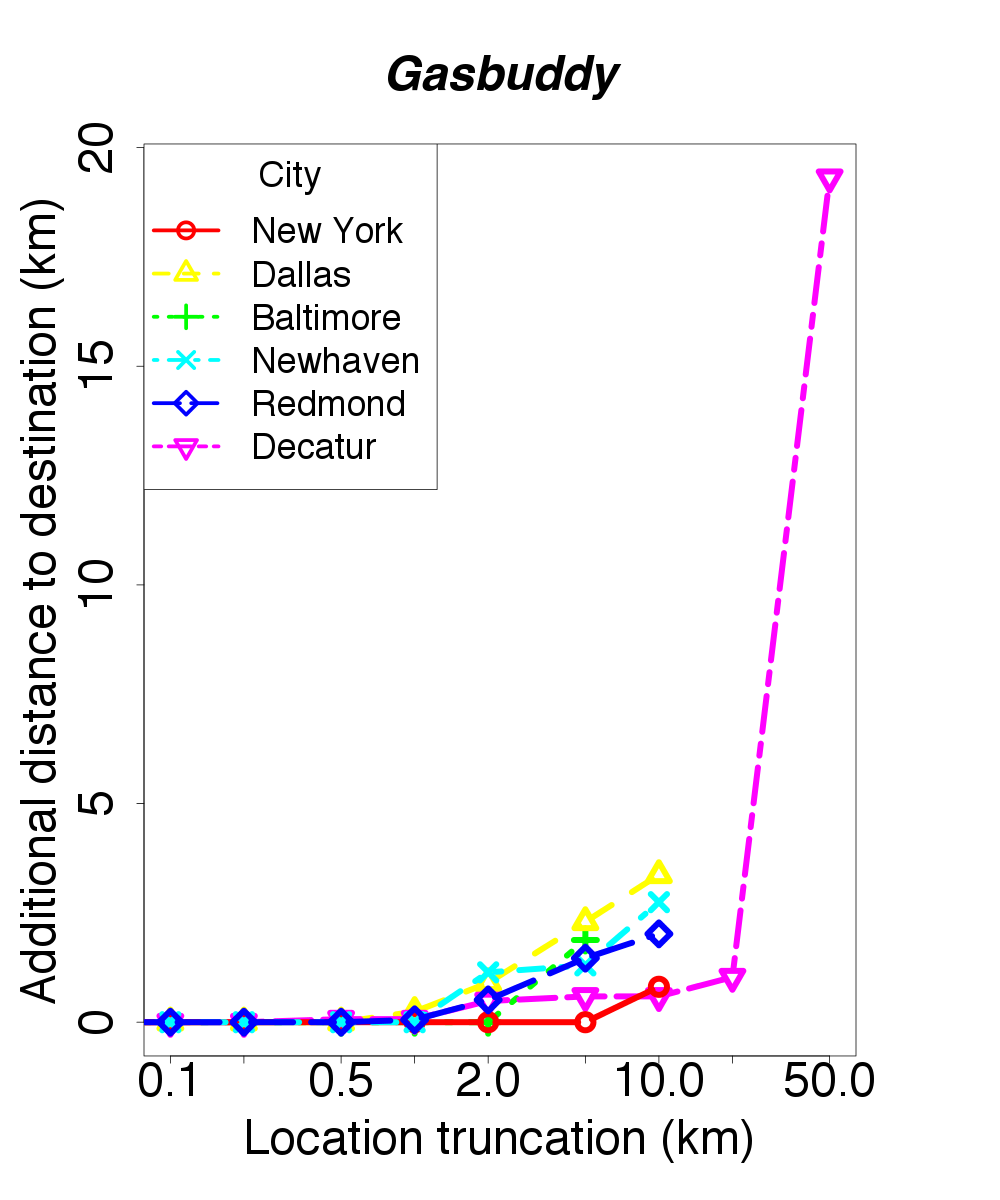
\includegraphics[width=\textwidth]
                      {location_privacy/data/gasbuddy/plots/medians_across_city_additional_distance}
    \end{minipage}
    
    % [width=.6\textwidth]
    \begin{minipage}{2in}
      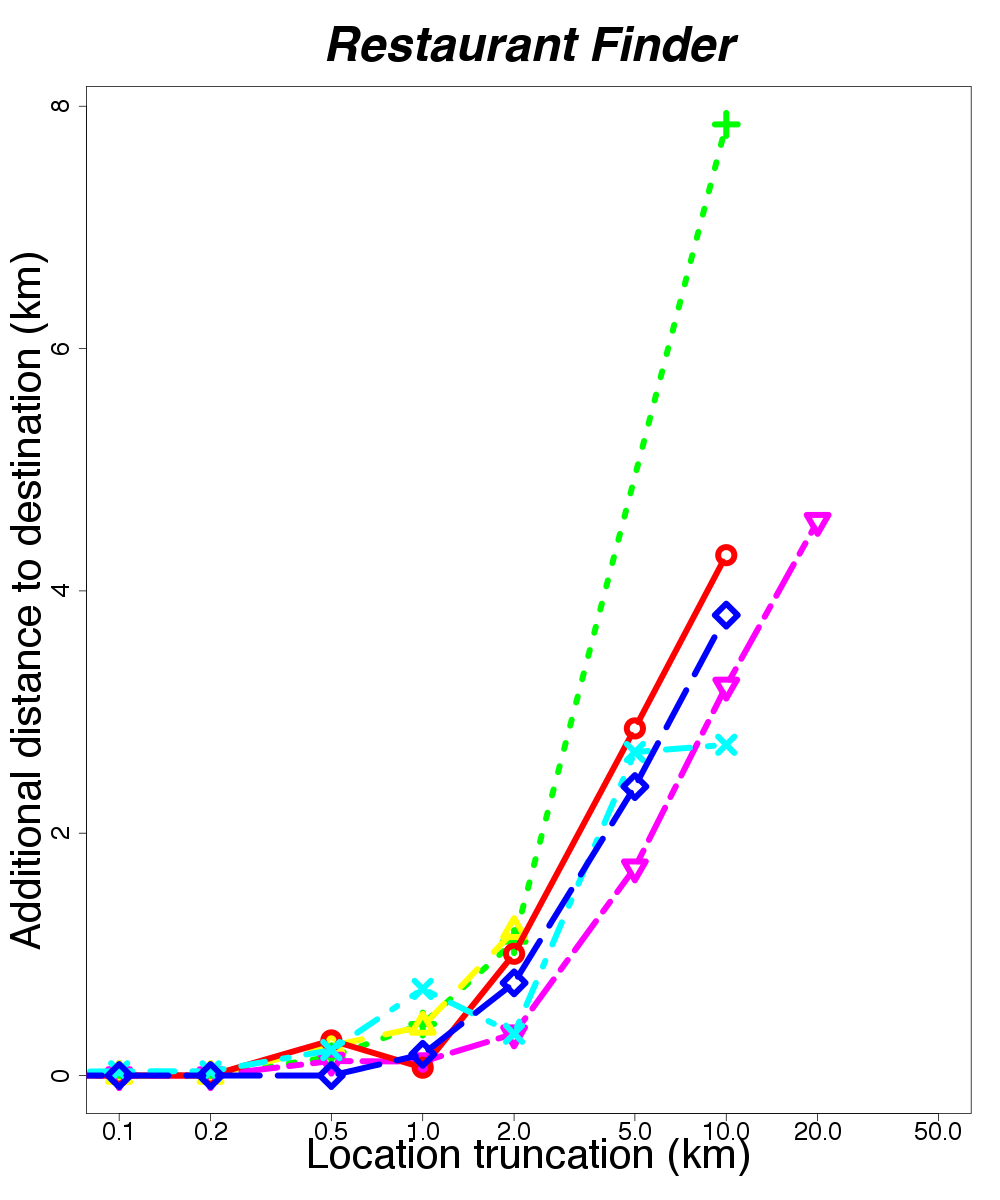
\includegraphics[width=\textwidth]
                      {location_privacy/data/restaurant_finder/plots/medians_across_city_additional_distance}
    \end{minipage}
    
    \begin{minipage}{2in}
      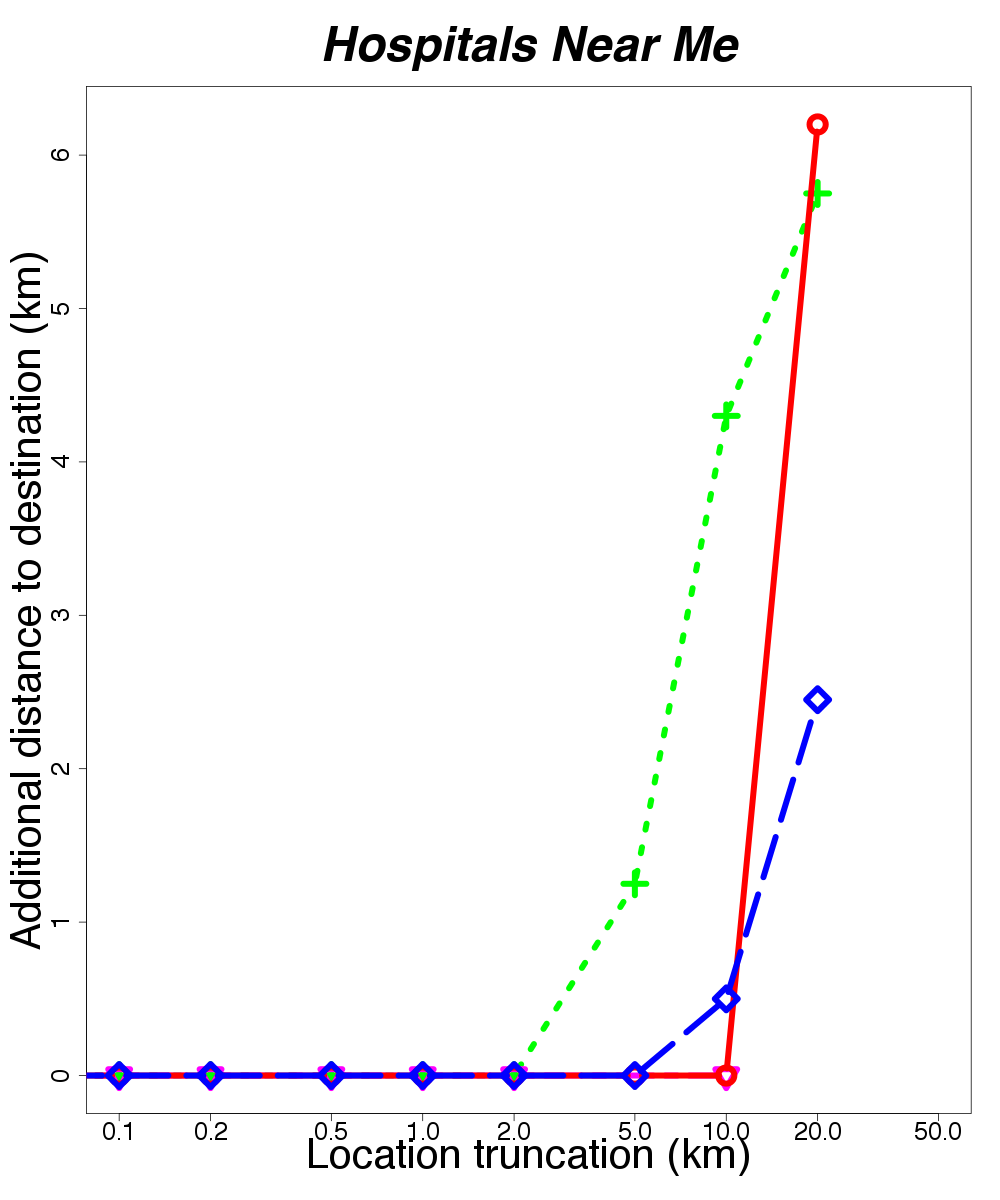
\includegraphics[width=\textwidth]
                      {location_privacy/data/hospitals/plots/medians_across_city_additional_distance}
    \end{minipage}
    
    \\
    \begin{minipage}{2in}
      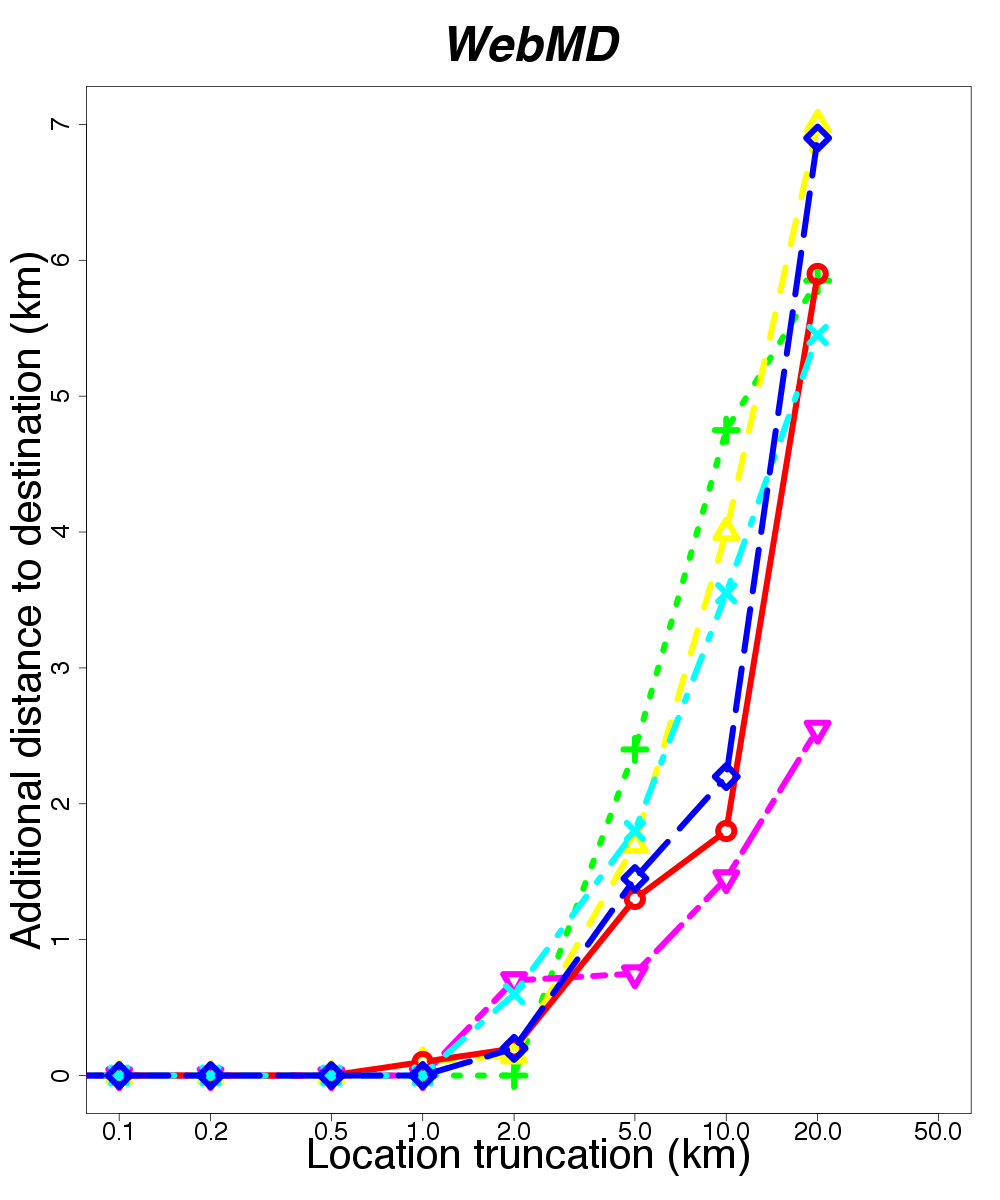
\includegraphics[width=\textwidth]
                      {location_privacy/data/webmd/plots/medians_across_city_additional_distance}
    \end{minipage}
    
    \begin{minipage}{2in}
      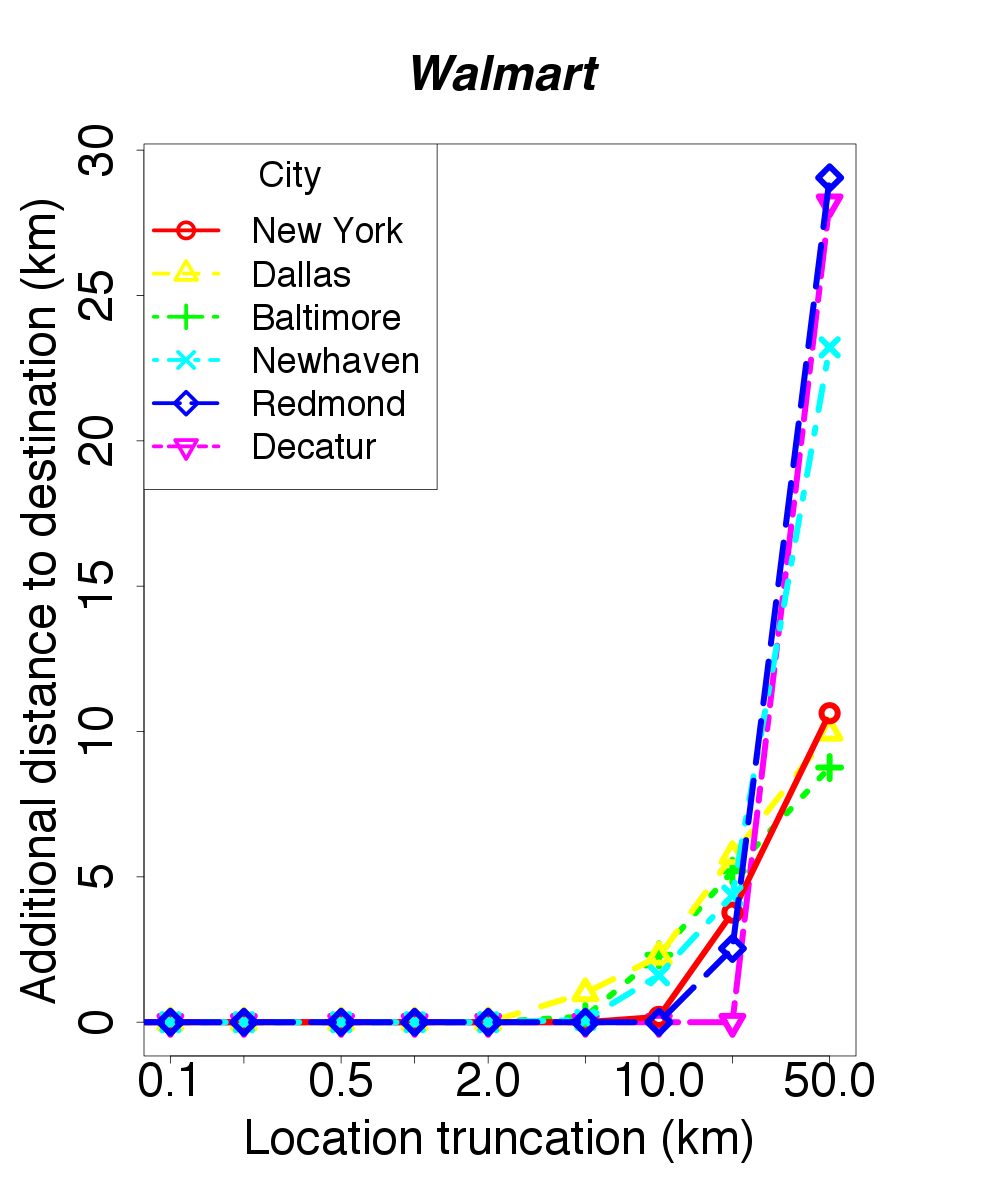
\includegraphics[width=\textwidth]
                      {location_privacy/data/walmart/plots/medians_across_city_additional_distance}
    \end{minipage}
    
    \begin{minipage}{2in}
      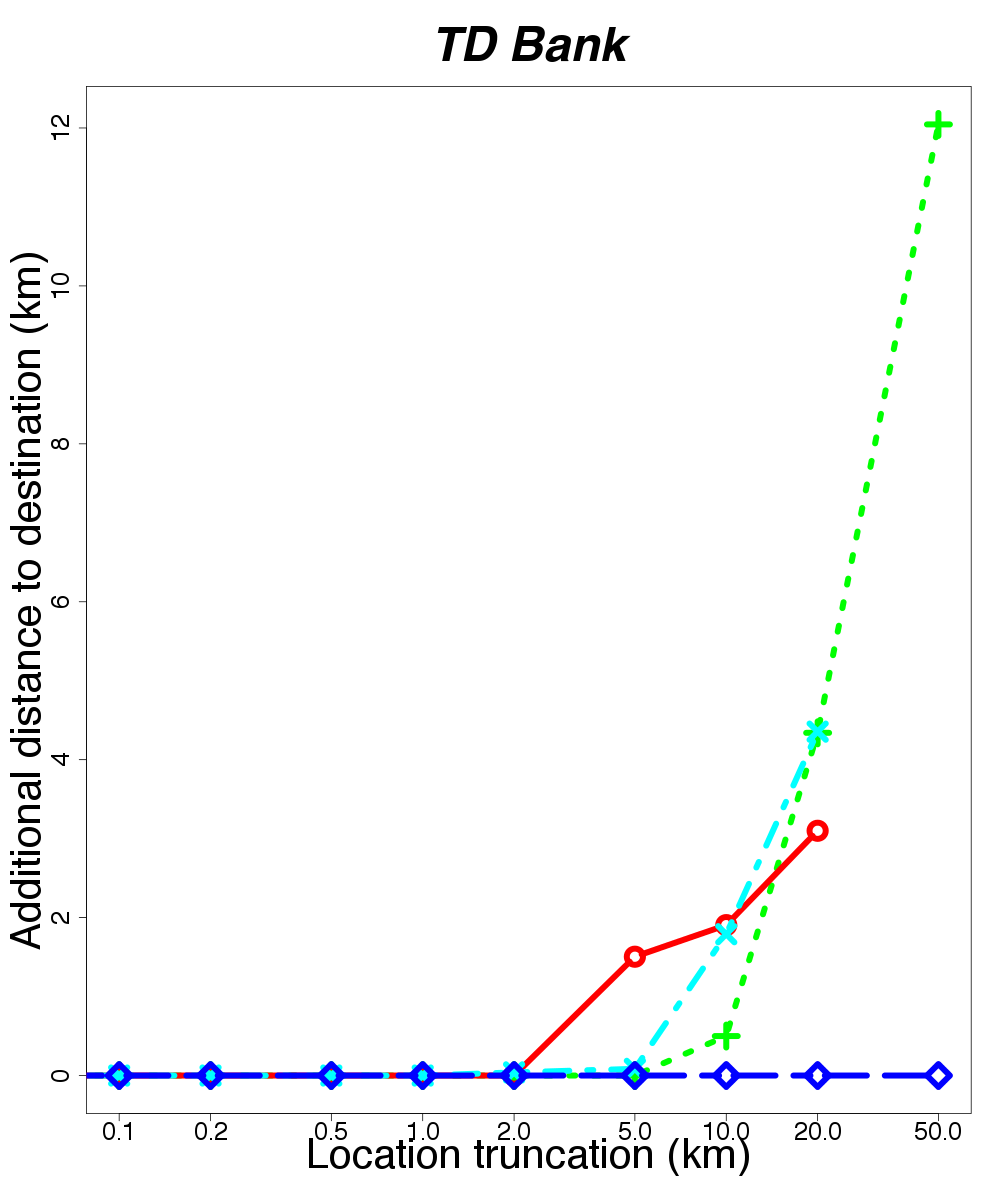
\includegraphics[width=\textwidth]
                      {location_privacy/data/tdbank/plots/medians_across_city_additional_distance}
    \end{minipage}
  \end{tabular}
  \caption{Graph of median additional distance versus
    truncation amount.  Higher additional distance implies lower
    utility.}
  \label{fig:add_distance}
  \end{subfigure}

  \bigskip{}

  \begin{subfigure}[t]{\textwidth}
 \small
 \centering
 \begin{tabular}{|l|rrrrrr|}
 \hline
 & New York & Dallas & Baltimore & New Haven & Redmond & Decatur \\
 \hline
 Gasbuddy & $\cdot$ & 5 & 5 & 2 & 5 & 20 \\
Restaurant Finder & 2 & 2 & 2 & 5 & 5 & 5 \\
Walmart & 20 & 5 & 10 & 10 & 20 & 50 \\
TD Bank & 5 & $\cdot$ & 20 & 10 & $\cdot$ & $\cdot$ \\
WebMD & 5 & 5 & 5 & 5 & 5 & 10 \\
Hospitals Near Me & 20 & $\cdot$ & 5 & $\cdot$ & 20 & $\cdot$ \\
\hline
\end{tabular}
\caption{Largest truncation amount (km) before median additional
  distance exceeds 1~km.}
 \label{fig:knee-points-additional-cutoff}

  \end{subfigure}

\caption{Additional distance results.}
  
\end{figure*}

\subsubsection{Set Intersection}

Figure~\ref{fig:set-intersection-metric} shows the results for the set
intersection size metric, with the $y$-axis the percentage of the set
intersection size compared to the original set size.
Figure~\ref{fig:knee-points-set-cutoff} shows the truncation amount
after which the set intersection percentage drops below 80\% of the
original value.  More precisely, let $I(s)$ be the median intersection
set size under truncation $s$, defined as $|L \cap L'|/|L|$ where $L$
is the list without truncation and $L'$ is the list with truncation
$s$. Then the chart lists the $s_i$ such that $I(s_i) \leq 0.8$ and
$I(s_{i+1}) > 0.8$, where $s_j$ is the sequence of location truncation amounts.

We observe that apps measuring less densely distributed locations can
be truncated more aggressively than those measuring more densely
distributed locations.
For example, we see that Gasbuddy and Restaurant Finder,
which both measure densely distributed objects,
can sustain some truncation, but their utility drops off much faster than the
other apps such as Hospitals Near Me. In the table, we see this again
in that Gasbuddy and Restaurant Finder drop
below a set intersection size of 80\% at a lower truncation amount compared to Hospitals Near Me.

One slightly surprising trend in the table is that for Restaurant
Finder, location can be truncated more in New York than in other
location, whereas we would expect the opposite due to its
high density of restaurants. Looking into the results in detail, we
discovered this occurred because of the large radius (20~km) we chose
for New York: Restaurants are
typically clustered in the city center and we chose
locations randomly within the radius, so a large radius reduced restaurant
density.

\subsubsection{Additional Distance}

Figure~\ref{fig:add_distance} shows the results for the additional
distance metric applied to our subject apps.
Figure~\ref{fig:knee-points-additional-cutoff} shows, for each city
and each app, the last truncation amount before median additional
distance degrades beyond 1~km. In other words, if we let
$\Delta(s)$ be the
median additional distance under truncation $s$, the chart lists
the $s_i$ such that $\Delta(s_i) \leq 1~km$ and $\Delta(s_{i+1}) >
1~km$.

Note that the additional distance is undefined if a location
truncation produces a new closest location that was not present in the
original output list, as in this case we cannot compute how far the
new closest location is from the current location. In the charts,
undefined additional distances are omitted, as thus some lines end
before reaching the maximum truncation. This also limits the number of
points on which we can compute the cutoff.  For example, the Gasbuddy
app never causes the user to go more than 1 km out of the way in New York, 
so it is listed as ``$\cdot$'' in Figure~\ref{fig:knee-points-additional-cutoff}.

From these plots, we see that under the additional distance
metric, there is typically no change in app utility up to 1 or 2~km
truncation. Notice that this is
quite different behavior than under the edit distance metric,
where the edit distance is nonzero even with small amounts of 
location truncation.

In most cases, the lack of change in additional distance is
meaningful, but in a few cases it only reveals the low density of
located objects. In particular, in Redmond, the TD Bank app can
sustain location truncation up to 50~km without any change, but
this occurs because the first result on the list is over 100 km~away. This
also happens in the Hospitals Near Me app, as there are relatively few
hospitals in any area.

Looking at Figure~\ref{fig:knee-points-additional-cutoff}, we see that
if a user is willing to go 1~km out of their way, then in most
locations apps can sustain truncation amounts of 5~km or
more. However, as with edit distance the effect is highly dependent on
object density, e.g., Gasbuddy and Restaurant Finder are limited to 5~km
truncation (except in Decatur, which has fewer gas
stations), whereas other apps can be truncated to higher levels.

\subsubsection{Discussion}

Each of the three metrics applies in a different situations: edit
distance for when an exact order is desired, set intersection for when
a user wants to find any number of locations close by, and additional
distance for when a user wants to find a nearest location to visit.
The general trend for all three are similar: the metrics are much
more forgiving in less dense areas, which makes intuitive sense. In
terms of absolute values of truncation that can be sustained, we see
that edit distance is the least permissive, as very small changes have
large effects. (We did not include a table like
Figure~\ref{fig:knee-points-additional-cutoff}
or~\ref{fig:knee-points-set-cutoff} for edit distance because we have
no intuition of what a reasonable cutoff would be.) The next most
restrictive metric is set intersection size, and the most permissive
metric is additional distance.

\section{Related Work}

Several other researchers have proposed mechanisms to refine or reduce
permissions in Android. MockDroid allows users to replace an
app's view of certain private data with fake
information~\cite{mockdroid}. Apex is similar, and also lets 
the user enforce simple constraints such as the
number of times per day a resource may be accessed~\cite{apex}. TISSA
gives users detailed control over an app's access to selected private data
(phone identity, location, contacts, and the call log), letting the
user decide whether the app can see the true data, empty data,
anonymized data, or mock data~\cite{zhou2011taming}. AppFence
similarly lets users provide mock data to apps requesting private
information, and can also ensure private data that is released to apps
does not leave the device~\cite{Hornyack:2011}.  A
limitation of all of these approaches is that they require
modifications to the Android platform, and hence to be used in
practice must either be
adopted by Google or device providers, or must be run on rooted
phones. In contrast, \rewriter and \lib run on stock, unmodified
Android systems available today.

Researchers have also developed other ways to enhance Android's
overall security framework. Kirin employs a set of user-defined
security rules to flag potential malware at install
time~\cite{enck2009lightweight}. Saint enriches permissions on Android
to support a variety of installation constraints, e.g., a permission
can include a whitelist of apps that may request
it~\cite{ongtang2009semantically}. These approaches are complementary
to our system, as they take the platform permissions as is and do not
refine them.

There have been several studies of Android's permissions, sensitive
APIs, and the use of permissions across apps.  Barrera et
al.~\cite{barrera2010methodology} analyze the way permissions are used
in Android apps, and observe that only a small number of Android
permissions are widely used but that some of these, in particular
Internet permissions, are overly broad (as we have also found). Vidas
et al.~\cite{vidas:w2sp11} describe a tool that, using
documentation-derived information, can statically analyze an app's
source code to find a minimum set of permissions it
needs. Stowaway~\cite{Felt:2011} performs a static analysis on the
Android API itself to discover which APIs require what permissions,
something they found is not always well documented. (We used
Stowaway's data set in several cases to help determine what adapters
we needed to implement in \lib.)

Finally, several tools have been developed that look for security
issues in Android apps. TaintDroid tracks the flow of sensitive
information~\cite{taintdroid}. Ded~\cite{ded}, a Dalvik-to-Java
decompiler, has been used to discover previously undisclosed device
identifier leaks. ComDroid~\cite{chin11:mobisys} finds vulnerabilities
related to Intent handling. Felt et al.~\cite{felt2011permission}
study the problem of permission redelegation, in which an app is
tricked into providing sensitive capabilities to another app.
Woodpecker~\cite{grace:ndss12} uses dataflow analysis to find
capability leaks on Android phones. All of these tools focus on
improper use of the current set of Android's permissions. \rewriter
and \lib take a complimentary approach, replacing existing permissions
with finer-grained ones to reduce or eliminate consequences of
security issues.

\paragraph*{Related Work for Location Privacy}

There is a large body of work on increasing location
privacy, though we are aware of no other work that directly measures
the resulting utility of mobile Android apps.

The Cach\'{e} system \cite{Amini:2010} caches and prefetches
content from a server, obfuscating the user's location at the cost of
potentially stale content and higher bandwidth.  Additionally,
application writers must specify rules for caching up front.  The
system caches data for a set of regions, quantizing the user's location 
as in our approach.  
The authors note that app utility will be impacted by their technique, 
but they do not measure it explicitly.

Hornyack et al. \cite{Hornyack:2011} study apps that use sensitive
information (such as location), and present AppFence, a system that
can fuzz inputs to apps. While the AppFence authors note the effects of
fuzzing app inputs on usability, they do not study it systematically
using any particular metric.

Shokri et al. \cite{Shokri:2011} present a systematic approach to
quantifying Location Privacy Preserving Mechanisms (LPPMs).  They also
describe an meter on the user's devise that
continuously informs the user of their privacy.  In our work, we implemented a simple
truncation-based LPPM (corresponding to a technique they call
\emph{precision reduction}), and use this to study
utility as a function of the degree of truncation. As future work, we
may consider evaluating the utility of other policies from their
system.

In follow up work, Shokri et al. \cite{Shokri:2012} present an
optimal strategy to prevent localization attacks.
%, based on bounding
%the probability that an attacker can learn the
%precise location of a user at a given time.  
Their analysis formulates location privacy as a Bayesian Stackelberg 
game, where a user chooses a location cloaking strategy without 
knowing their potential adversary.
While their analysis considers service quality, they use metrics that do 
not clearly map to utility, such as Euclidean distance from the 
true location (rather than the actual effect of the change on the service).

Our study focuses on privacy for a single user at a stationary point.
Allowing the app to collect traces of data reveals much more
information \cite{Gruteser:2005}, \cite{Golle:2009}.  Much of the
existing work on location privacy \cite{Beresford:2004}, \cite{Bettini:2005},
\cite{Hoh:2005}, \cite{Gruteser:2003} focuses on $k$-anonymity: if a
user is making a query to a location based service, they can only be
identified to be within a set of $k$ potential users.  
One popular
technique is to use mix zones \cite{Beresford:2004}: once a user enters 
a designated area their location information becomes ``mixed'' with 
others in that same area.  This technique requires a trusted middleware 
layer (to properly mix location data) and requires these mix zones 
to be defined.  In contrast, location truncation can be done locally
on a mobile device.

None of these previous approaches study the impact of location privacy
on app utility.  The work that comes closest is by Shokri et
al. \cite{Shokri:2012}, but while that framework considers utility as
an element of their models, it is not directly measured on apps.  Our
work is complementary: we focus not on optimal obfuscation techniques,
but rather we fix an obfuscation strategy and study how utility
changes under that technique.  As future work, we intend to couple our 
empirical utility functions with the theoretical models presented by
Shokri et al.
Doing so would allow us to determine bounds for $k$ and allow us to study 
how the optimal strategies presented by Shokri et al.
are affected.

\section{Conclusion}

We presented an empirical study of how location truncation affects
mobile app utility. We began by examining how Android apps use
location. Across the apps we looked at, we found that the second most
common pattern is using the current location to list various sorts of
nearby objects. The most common pattern, location-targeted ads, is not
amenable to evaluating utility. We then used Dr.~Android and Mr.~Hide
to implement \fuzzer{}, a tool that
modifies existing apps' bytecode to use truncated location
information. We designed an experiment in which we measured the effect
of a range of location truncations (from 0~km to 50~km) on 60
points randomly chosen from various locales (from population 6,000
Decatur, TX to population 8.2 million New York, NY). We identified three
metrics that approximate app utility: edit distance, set intersection
size, and additional distance. We found that, under these metrics, the
factor that most determines the utility--truncation tradeoff is
the density of objects being returned by the app, and that in many
cases, location can be truncated significantly without losing much
utility. To our knowledge, our work provides the first end-to-end
evaluation of how location truncation affects Android app utility.
As subject of future work, we plan to apply CloakDroid to a larger 
number of apps and test the metrics using user studies.


%% \begin{abstract} 
%%   Mobile apps can access a wide variety of secure information, such as
%%   contacts and location. However, current mobile platforms include
%%   only coarse access control mechanisms to protect such data.  In this
%%   paper, we introduce \emph{interaction-based declassification
%%     policies}, in which the user's interactions with the app constrain
%%   the release of sensitive information.  Our policies are defined
%%   extensionally, so as to be independent of the app's implementation,
%%   based on sequences of security-relevant events that occur in app
%%   runs. Policies use LTL formulae to precisely specify which secret
%%   inputs, read at which times, may be released. We formalize a
%%   semantic security condition, \emph{interaction-based
%%     noninterference}, to define our policies precisely.  Finally, we
%%   describe a prototype tool that uses symbolic execution of Dalvik bytecode to check
%%   interaction-based declassification policies for Android, and we show
%%   that it enforces policies correctly on a set of apps.
%%   \keywords{Information flow, program analysis, symbolic
%%     execution.}
%% \end{abstract}

\renewcommand{\thechapter}{3}

\chapter{Checking Interaction-Based Declassification Policies \\
  for Android Using Symbolic Execution}

\lstset{language=Java,
  morecomment=[l]{--},          % add Haskell comment style
  columns=flexible,
  basicstyle=\footnotesize\sffamily,
  literate={->}{$\rightarrow$}2
           {=>}{$\Rightarrow$}2
           {<-}{$\leftarrow$}2
           {...}{$\ldots$}2
           {fun}{$\lambda$}1
           {||}{$\parallel$}1
           {**}{$\times$}2,
  escapechar=@,
  escapeinside={/**}{*/},
  numbers=left,                   % where to put the line-numbers
  numberstyle=\tiny\color{gray},  % the style that is used for the line-numbers
  stepnumber=1,                   % the step between two line-numbers. If it's 1, each line 
                                  % will be numbered
  numbersep=5pt,                  % how far the line-numbers are from the code
  showspaces=false,               % show spaces adding particular underscores
  showstringspaces=false,         % underline spaces within strings
  numberblanklines=false,
  showtabs=false,
  frame=single,                   % adds a frame around the code
  rulecolor=\color{gray},        % if not set, the frame-color may be changed on line-breaks within not-black text (e.g. commens (green here))
  commentstyle=\color{dkred}\itshape,       % comment style
  stringstyle=\color{mauve}         % string literal style
}

The last chapter introduced Redexer, a tool that allows binary
rewriting of Android apps. Redexer allows us to change the dynamic
behavior of an Android app, e.g., to change the way it uses
permissions. However, manipulating the way an app accesses information
does not allow us to understand what is done with the information once
it enters the app. In this chapter, I describe how to check
\emph{information flow} properties using a static analysis. In doing
so, I detail a novel policy framework that allows reasoning about how
UI interactions can be used to declassify information.

\section{Introduction}
\label{sec:introduction}

The Android platform includes a \emph{permission} system that aims to
prevent apps from abusing access to sensitive information, such as
contacts and location. Unfortunately, once an app is installed, it has
\emph{carte blanche} to use any of its permissions in arbitrary ways
at run time. For example, an app with location and Internet access
could continuously broadcast the device's location, even if such
behavior is not expected by the user.
%Thus, permissions do not enable fine-grained control of what and when
%sensitive information may be used.

To address this limitation, I present a new framework for Android app
security based on \emph{information flow control} \cite{Denning:1975}
and user interactions.  The key idea behind our framework is that
users naturally express their intentions about information release as
they interact with an app.  For example, clicking a button may permit
an app to release a phone number over the Internet. Or, as another
example, toggling a radio button from ``coarse'' to ``fine'' and back
to ``coarse'' may temporarily permit an app to use fine-grained GPS
location rather than a coarse-grained approximation.

To model these kinds of scenarios, we introduce
\emph{interaction-based declassification policies}, which
extensionally specify what information flows may occur after which
sequences of \emph{events}.  Events are GUI interactions (e.g.,
clicking a button), inputs (e.g., reading
the phone number), or outputs (e.g., sending over the Internet).
A policy is a set of \emph{declassification conditions}, written
$\phi \mathrel\rhd S$, where $\phi$ is a linear-time temporal logic
(LTL)~\cite{Pnueli:1977} formula over events, and $S$ is a sensitivity
level.  If $\phi$ holds at the time an input occurs, then that input
is declassified to level $S$. 
We formalize a semantic security condition,
\emph{interaction-based noninterference} (IBNI), over sets of event
\emph{traces} generated by an app.  Intuitively, IBNI holds of an app
and policy if observational
determinism~\cite{Zdancewic:03} holds after all inputs have been
declassified according to the policy. 
(Section~\ref{sec:overview}
describes policies further, and Section~\ref{sec:formalism} presents
our formal definitions.)

We introduce \toolname, a static analysis tool to check
whether an Android app and its declassification policy
satisfy IBNI.
\toolname generates event traces using SymDroid~\cite{Jeon:2012}, a
Dalvik bytecode symbolic executor.  \toolname
works by simulating user interactions with the app and recording the
resulting execution traces.
In practice, it is not feasible to
enumerate all program traces, so \toolname generates traces up to some
\emph{input depth} of $n$ GUI events.  
\toolname{} then synthesizes a
set of logical formulae that hold if and only if IBNI holds, and uses
Z3~\cite{deMoura:2008} to check their satisfiability.
(Section~\ref{sec:implementation} describes \toolname in detail.)

To validate \toolname, we used it to analyze four Android apps,
including both secure and insecure variants of those apps.
We ran each app variant under a range of input depths, and confirmed
that, as expected, \toolname{} scales exponentially.
However, we manually examined each app and its policy, and
found that an input depth of at most 5 is sufficient to
guarantee detection of a security policy violation (if any) for these
cases.  We ran \toolname{} at these minimum input depths and found
that it correctly passes and fails the secure and insecure app
variants, respectively. Moreover, at these depths, \toolname{} takes just a few
seconds to run. (Section~\ref{sec:experiments} describes our experiments.)

In summary, we believe that \toolname takes an important step forward
in providing powerful new security mechanisms for mobile devices. We
expect that our approach can also be used in other
GUI-based, security-sensitive systems.

\section{Example Apps and Policies}
\label{sec:overview}

We begin with two example apps that show interesting aspects of
interaction-based declassification
policies.

\paragraph*{Bump app.}

The boxed portion of Fig.~\ref{fig:app-bump} gives (simplified) source
code for an Android app that releases a device's unique ID and/or phone
number. This app is inspired by the Bump app, which let users tap
phones to share selected information with each other.  We have
interspersed an insecure variant of the app in the red code on
lines~\ref{line:bump1} and \ref{line:bump2}, which we will
discuss in Section~\ref{sec:traces}.

Each screen of an Android app is implemented using a class that
extends \code{Activity}. When an app is launched, Android invokes the
\code{onCreate} method for a designated main activity.
(This is part of the \emph{activity lifecycle}~\cite{Android:15},
which includes several methods called in a certain order. For this
simple app, and the other apps used in this chapter, we only need a
single activity with this one lifecycle method.)
That method retrieves
(lines~\ref{line:bump-button}--\ref{line:bump-check}) the GUI IDs of a
button (marked ``send'') and
two checkboxes (marked ``ID'' and ``phone''). The \code{onCreate} method next
gets an instance of the \code{TelephonyManager}, uses it
to retrieve the device's unique ID and phone number information, and unchecks the two
checkboxes as a default. Then it creates a new callback
(line~\ref{line:bump-cb}) to be invoked when the ``send'' button is
clicked. When called, that callback releases the user's ID and/or
phone number, depending on the checkboxes.

\begin{figure}[t]
  \centering
  %\begin{tabular}{ccc}
  %\begin{minipage}[c]{0.45\textwidth}
  \begin{lstlisting}[name=Ex]
    public class BumpApp extends Activity {
      protected void onCreate(...) {
        Button sendBtn = (Button) findViewById(...); /**\label{line:bump-button}*/
        CheckBox idBox = (CheckBox) findViewById(...);
        CheckBox phBox = (CheckBox) findViewById(...);/**\label{line:bump-check}*/
        TelephonyManager manager = TelephonyManager.getTelephonyManager(); /**\label{line:bump-tele}*/
        final int id = manager.getDeviceId(); /**\label{line:bump-id}*/
        final int ph = manager.getPhoneNumber();
        idBox.setChecked(false); phBox.setChecked(false);
        sendBtn.setOnClickListener(
        new OnClickListener() { /**\label{line:bump-cb}*/
          public void onClick(View v) {
            if (idBox.isChecked())
            Internet.sendInt(id); /**\textcolor{red}{//Internet.sendInt(ph);}\label{line:bump1}*/
            if (phBox.isChecked())
            Internet.sendInt(ph); /**\textcolor{red}{//Internet.sendInt(id);}\label{line:bump2}*/
        }})}}
  \end{lstlisting}
  \begin{displaymath}
    \begin{array}{cc}
      \code{id}!\ast \wedge (\tfuture ( \code{sendBtn!unit} \land
      \tlast{\code{idBox}}{\code{true}})) \rhd Low, \\

      \code{ph}!\ast \wedge (\tfuture (
      \code{sendBtn!unit} \land
      \tlast{\code{phBox}}{\code{true}})) \rhd Low \\
    \end{array}
  \end{displaymath}
  \caption{``Bump'' app and policy.}
  \label{fig:app-bump}
  %\end{minipage}
  % &
  %\hspace*{0.01\textwidth}
  %&
  %\begin{minipage}[c]{0.45\textwidth}
  %\end{minipage}
  %\end{tabular}
  %\caption{Example apps.}
\end{figure}

This app is written to work with \toolname{}, a symbolic execution tool we built to check
whether apps satisfy interaction-based declassification policies. As we
discuss further in Section~\ref{sec:implementation}, \toolname{} uses an
executable model of Android that abstracts away some details that are
unimportant with respect to security. While a real app would release
information by sending it to a web server, here we instead call a
method \code{Internet.sendInt}. Additionally, while real apps
include an XML file specifying the screen layout of buttons,
checkboxes, and so on, \toolname{} creates those GUI elements
on demand at calls to \code{findViewById} (since their screen locations are
unimportant). Finally, we model the ID and phone number as
integers to keep the analysis simpler.

\toolname{} symbolically executes paths through subject apps, recording a
\emph{trace} of \emph{events} that correspond to certain method calls.
For example, one path through this app generates a trace
\begin{displaymath}
  \code{id!42}, \code{ph!43}, \code{idBox!true},
  \code{sendBtn!unit}, \code{netout!}\code{42}
\end{displaymath}
Each event has a \emph{name} and a \emph{value}. Here we have used
names \code{id} and \code{ph} for secret inputs, \code{idBox} and
\code{sendBtn} for GUI inputs, and \code{netout} for the network
send.  In particular, the trace above indicates 42 is read as the ID,
43 is read as the phone number, the ID checkbox is selected, the send
button is clicked (carrying no value, indicated by
\code{unit}), and then 42 is sent on the network. In \toolname{},
events are generated by calling certain methods that are specially
recognized. For example, \toolname{} implements the
\code{manager.getDeviceId} call as both returning a value and emitting
an event.

Notice here that in the trace, callbacks to methods such as
\code{idBox} and \code{sendBtn} correspond to user
interactions. The key idea behind our framework is that these actions
convey the user's intent as to which information should be
released. Moreover, traces also contain actions relevant to
information release---here the reads of the ID and phone number, and
the network send. Thus, putting both user interactions and
security-sensitive operations together in a single trace allows
our policies to enforce the user's intent.

The policy for
this example app is shown at the bottom of Fig.~\ref{fig:app-bump}.
Policies are comprised of a set of \emph{declassification
  conditions} of the form $\phi \rhd S$, where $\phi$ is an LTL
formula describing event traces and $S$ is a security level.  Such a
condition is read, ``At any input event, if $\phi$ holds at that
position of the event trace, then that input is declassified at level
$S$.''  For this app there are two declassification conditions. The
top condition declassifies (to \emph{Low}) an input that is a
read of the ID at any value (indicated by $\ast$), if
sometime in the future (indicated by the $\tfuture$ modality) the send
button is clicked and, when that button is clicked, the last value of
the ID checkbox was \code{true}. (Note that \emph{last} is not
primitive, but is a macro that can be expanded into regular LTL.)  The
second declassification condition does the analogous thing for the
phone number.

To check such a policy, \toolname{} symbolic executes the program,
generating per-path traces; determines the classification level of every input; and
checks that every pair of traces satisfies noninterference.
Note that using LTL provides a very general and
expressive way to describe the sequences of events that imply
declassification. For example, here we precisely capture that
only the last value of the checkbox matters for declassification. For
example, if a user selects the ID checkbox but then unselects it
and clicks send, the ID may not be released.

Although this example relies on a direct flow, \toolname{} can also
detect implicit flows. Section~\ref{sec:policies} defines an
appropriate version of noninterference, and the experiments in
Section~\ref{sec:experiments} include a subject program with an
implicit flow.

% In this example, we have stored the device id in the \code{id}
% variable.  But our policy would work even if the program had (e.g.)
% stored it in a database (though our system model does not include
% databases at this time), or transforming the data and then later
% sending it.  This is because our system reasons about information
% flow, rather than simply data flow.

Notice this policy depends on the app reading the ID
and phone number when the app starts. If the app instead
waited until after the send button were clicked, it would violate this
policy. We could address this by replacing the $\tfuture$ modality by
$\tpast$ (past) in the policy, and we could form a disjunction of the
two policies if we wanted to allow either implementation. More generally, we
designed our framework to be sensitive to such choices to
support  reasoning about secret
values that change over time. We will see an
example next.

\paragraph*{Location resolution toggle app.}

\begin{figure}[t]
  \centering
  \begin{lstlisting}[name=Ex]
    public class ToggleRes extends Activity { ...
      LocSharer mLocSharer = new LocSharer();
      RadioManager mRadio = new RadioManager();
      protected void onCreate(...) { ... }
      private class LocSharer implements LocationListener { ... 
        public LocSharer(RadioManager rm) {
          lm = (LocationManager) getSystemService(LOCATION_SERVICE);
          lm.requestLocationUpdates(mCurrentProvider, SHARE_INTERVAL, distance, this);
        }
        public void onLocationChanged(Location l) {
          if (mRadio.mFine) {
            Internet.sendInt(l.mLatitude);
            Internet.sendInt(l.mLongitude);
          } else {
            Internet.sendInt(l.mLatitude & 0xffffff00);
            Internet.sendInt(l.mLongitude & 0xffffff00);
      } } }
      private class RadioManager
      implements OnClickListener {
        public boolean mFine = false;
        public void onClick(View v) { mFine = !mFine; }
    } }
  \end{lstlisting}
  \begin{displaymath}
    \begin{array}{ll}
      \code{longitude}!\ast \wedge
      \tlast{\code{mRadio}}{\code{true}} \rhd
      \textit{Low}, \\
      \code{longitude}!\ast \wedge
      \tlast{\code{mRadio}}{\code{false}} \rhd
      \textit{MaskLower8}
    \end{array}
  \end{displaymath}
  \caption{Location sharing app and policy.}
  \label{fig:app-loc-toggle}
\end{figure}

Fig.~\ref{fig:app-loc-toggle} gives code for an app that
shares location information, either at full or truncated resolution
depending on a radio button setting. The app's \code{onCreate}
method displays a radio button (code not shown) and then creates and
registers a new instance of \code{RadioManager} to be called
each time the radio button is changed. That
class maintains field \code{mFine} as \code{true} when the radio button is
set to full resolution and \code{false} when set to truncated
resolution.

Separately, \code{onCreate} registers \code{LocSharer} to be called
periodically with the current location.  It requests location updates
by registering a callback with the \code{LocationManager}
system service.  When called, \code{LocSharer} releases the
location, either at full resolution or with the lower 8 bits
masked, depending on \code{mFine}.

The declassification policy for longitude appears below the code; the
policy for latitude is analogous.  This policy allows the precise
longitude to be released when
\code{mRadio} is set to fine, but only the lower eight bits to
be released if \code{mRadio} is set to coarse. Here \toolname{}
knows that at the \textit{MaskLower8} level, it should consider
outputs to be equivalent up to differences in the lower 8
bits. 

Finally, notice that this policy does not use the future
modality. This is deliberate, because location may be read multiple
times during the execution, at multiple values, and the security level
of those locations should depend on the state of the
radio button at that time. For example, consider a trace
\begin{displaymath}
  \code{mRadio!false}, \code{longitude!}v_1,
  \code{mRadio!true}, \code{longitude!}v_2
\end{displaymath}
The second declassification condition ($\code{longitude}!\ast \wedge
\tlast{\code{mRadio}}{\code{false}}$) will match the event with $v_1$, since
the last value of \code{mRadio} was \code{false}, and
thus $v_1$ may be declassified only to \textit{MaskLower8}. Whereas
the first declassification condition will match the event with $v_2$, hence it
may be declassified to \textit{Low}.

\section{Program Traces and Security Definition}
\label{sec:formalism}

Next, we formally define when a set of program traces satisfies an
interaction-based declassification policy.

\subsection{Program Traces}
\label{sec:traces}

\begin{figure}[t!]
  \small
  \centering
  \begin{displaymath}
    \begin{array}{p{1in}lrl}
      Primitives & \xv & ::= & n \mid \strue \mid \sfalse \mid \sunit \mid f(\xv_1, \ldots, \xv_i) \\
      Events & \evt & ::= & \sch ! p \\
      Traces & t & ::= & \evt ~ \textit{list} \\
      \\
      \multicolumn{4}{c}{\textrm{(a) Event and Trace Definitions.}} \\
      \\
      Policies & P & ::= & C_1, C_2, \ldots \\
      Conditions & C & ::= & \phi \rhd S\\
      Security Levels & S & ::= & \textit{High} \mid \textit{Low} \mid
      \textit{MaskLower8} \mid \ldots \\
      Atoms & \atom & ::= & \sch!s \mid s \oplus s \\
      Messages & s & ::= & x \mid p \mid \ast \\
      Formulae & \phi & ::= &
      \atom
      \mid \neg \phi
      \mid \phi \wedge \phi
      \mid \phi \vee \phi
      \mid \phi \limplies \phi
      \mid \exists x.\phi 
      \mid \forall x.\phi \\
      && \mid  & \tnext \phi
      \mid \phi \tuntil \phi
      \mid \talways \phi
      \mid \tfuture \phi
      \mid \phi \tsince \phi
      \mid \tpast \phi \\
      \\
      \multicolumn{4}{c}{\textrm{(b) Interaction-based Declassification Policy Language.}}
    \end{array}
  \end{displaymath}
  \caption{Formal definitions.}
  \label{fig:formalism}
\end{figure}

Fig.~\ref{fig:formalism}(a) gives the formal syntax of events and
traces.  \emph{Primitives}~$p$ are terms that can be carried by
events, e.g., values for GUI events, secret inputs, or network
sends.  In our formalism, primitives are integers, booleans, and terms
constructed from primitives using uninterpreted constructors $f$.  As
programs execute, they produce a \emph{trace}~$\tr$ of
\emph{events}~$\evt$, where each event $\sch!p$ pairs an event name
$\sch$ with a primitive $p$. We assume event names are partitioned
into those corresponding to inputs and those corresponding to
outputs. For all the examples in this chapter, all names are inputs
except \code{netout}, which is an output.

Due to space limitations, we omit details of how traces are
generated.  These details, along with definition of our LTL 
formulas, can be found in a companion tech report \cite{Micinski:2015}.
Instead, we simply assume there exists some set
$\tset$ containing all possible traces a given program may
generate.
For example, consider the insecure variant bump app in
Fig.~\ref{fig:app-bump}, which replaces the black code with the red
code on lines lines \ref{line:bump1}
and \ref{line:bump2}.  This app sends the phone number when the
email box is checked and vice-versa. Thus, its set $\tset$
contains, among others, the following two traces:
\begin{displaymath}
  \begin{array}{cl}
    \code{id}!0, \code{ph}!0, \code{idBox}!\code{true},
    \code{sendBtn}!\code{unit}, \code{netout}!0 & (1) \\
    \code{id}!0, \code{ph}!1, \code{idBox}!\code{true},
    \code{sendBtn}!\code{unit}, \code{netout}!1 & (2) \\
  \end{array}
\end{displaymath}%
\lstset{language=Java}%
In the first trace, ID and phone number are read as 0, the
ID checkbox is selected, the button is clicked, and 0 is sent.
The second trace is similar, except the phone number and sent value
are 1. Below, we use these traces to show this program
violates its security policy.

\subsection{Interaction-based Declassification Policies}
\label{sec:policies}

We now define our policy language precisely.
Fig.~\ref{fig:formalism}(b) gives the formal syntax of
declassification policies.  A policy $P$ is a set of
\emph{declassification conditions} $C_i$ of the form $\phi_i\rhd S_i$,
where $\phi_i$ is an LTL formula describing when an input is
declassified, and $S_i$ is a \emph{security level} at which the value
in that event is declassified.

As is standard, security levels $S$ form a lattice.  For our
framework, we require that this lattice be finite.  We include
\textit{High} and \textit{Low} security levels, and we can generalize
to arbitrary lattices in a straightforward way. Here we include the
\textit{MaskLower8} level from Fig.~\ref{fig:app-loc-toggle} as an
example, where $\textit{Low} \sqsubseteq \textit{MaskLower8}
\sqsubseteq \textit{High}$.  Note that although we include
\textit{High} in the language, in practice there is no reason to
declassify something to level \textit{High}, since then it remains
secret.

The \emph{atomic predicates}~$A$ of LTL formulae match events,
e.g., atomic predicate $\sch!p$ matches exactly that event.
We include $\ast$ for matches to
arbitrary primitives. We allow event values to be
variables that are bound in an enclosing quantifier. The atomic
predicates also include atomic arithmetic
statements; here $\oplus$ ranges over standard operations such as $+$,
$<$, etc.  
The combination of these lets us describe complex
events. For example, we could write
$\exists x. \textit{spinner}!x \wedge x > 2$ to indicate the
\emph{spinner} was selected with a value greater than 2.

Atomic predicates are combined with the usual boolean connectives
($\neg$, $\wedge$, $\vee$, $\rightarrow$) and existential and
universal quantification.  Formulae include standard LTL
modalities $\tnext$ (next), $\tuntil$
(until), $\talways$ (always), $\tfuture$ (future), $\phi \tsince \psi$
(since), and $\tpast \phi$ (past). We include a wide range of
modalities, rather than a minimal set, to make policies easier to write.
Formulae also include
$\tlast{\sch}{p}$, which is syntactic sugar for $\lnot (\sch!\ast)
\tsince \sch!p$.
We assume a standard interpretation of LTL formulae over
traces \cite{Lichtenstein:85}.
We write $\tr, i \models \phi$ if trace $\tr$ is a model of $\phi$ at
position $i$ in the trace.

% \begin{figure}[!t]
%   \small
%   \begin{displaymath}
%     \begin{array}{rcl}
%       P & ::= & C_1, C_2, \ldots \\
%       C & ::= & \phi \rhd S\\
%       S & ::= & \textit{High} \mid \textit{Low} \mid
%       \textit{MaskLower8} \mid \ldots \\
%       \atom & ::= & \sch?s \mid \sch!s \mid s \oplus s \\
%       s & ::= & x \mid p \mid \ast \\
%       \phi & ::= &
%       \atom
%       \mid \neg \phi
%       \mid \phi \wedge \phi
%       \mid \phi \vee \phi
%       \mid \phi \limplies \phi
%       \mid \exists x.\phi 
%       \mid \forall x.\phi
%       \mid  \tnext \phi
%       \mid \phi \tuntil \phi
%       \mid \talways \phi
%       \mid \tfuture \phi
%       \mid \phi \tsince \phi
%       \mid \tpast \phi \\
%     \end{array}
%   \end{displaymath}
%   \caption{GUI-based Declassification Policy Language.}
%   \label{fig:policy-temporal-logic}
% \end{figure}

% \begin{displaymath}
%   \begin{array}{c}
%     \code{email}?v \land \big( \tfuture ( \code{button} = () \land 
%     last(\code{email\_released})=\code{true} \big) \rhd L, \\

%     \code{email}?v \land \big( \tfuture ( \code{button} = () \land 
%     last(\code{email\_released})=\code{true} \big) \rhd L, \\
%   \end{array}
% \end{displaymath}

Next consider a trace $\tr \in \tset$ for an arbitrary program.
We write $\tlevel{\tr}{P}{i}$ for the security level that policy
$P$ assigns to the event $\tr[i]$:

\begin{displaymath}
  \tlevel{\tr}{P}{i} =
  \begin{cases}
    \bigsqcap_{\phi_j\rhd S_j \in P} \aset{ S_j \mid \tr, i \models
      \phi_j } & \tr[i] = \sch!p \\
    \textit{Low} & \tr[i] = \code{netout}!p \\
  \end{cases}
\end{displaymath}

In other words, for inputs, we take the greatest lower bound (the most
declassified) of the levels from all declassification conditions that
apply. We always consider network outputs to be
declassified. Notice that if no policy applies, the level is $H$ by
definition of greatest lower bound.

For example, consider trace (1) above with
respect to the policy in Fig.~\ref{fig:app-bump}.  At position 0, the
LTL formula holds because the ID box is eventually checked and then
the send button is clicked, so $\tlevel{(1)}{P}{0} =
\textit{Low}$. However,
$\tlevel{(1)}{P}{1} = \textit{High}$ because no
declassification condition applies for \code{ph}
(\code{phBox} is never checked). And $\tlevel{(1)}{P}{4} =
\textit{Low}$, because that position is a network send.

Next consider applying this definition to the GUI inputs. As written,
we have $\tlevel{(1)}{P}{2}$ = $\tlevel{(1)}{P}{3}$ =
\textit{High}. However, our app is designed to leak these inputs. 
For example, an adversary will learn the state of
\code{idBox} if they receive a message with an ID. Thus,
for all the subject apps in this chapter, we also declassify all GUI inputs as
\textit{Low}. 
For the example in Fig.~\ref{fig:app-bump}, this means
adding the conditions
$\code{idBox!}\ast \rhd \textit{Low}$,
$\code{phBox!}\ast \rhd \textit{Low}$, and
$\code{sendBtn!}\ast \rhd \textit{Low}$. In general, 
the security policy designer should decide the security level of GUI inputs.

Next, we can apply \textit{level} pointwise across a trace and discard
any trace elements that are below a given level $S$. We define
\begin{displaymath}
  \tleveltr{\tr}{P}^S[i] =
  \begin{cases}
    \tr[i] & \tlevel{\tr}{P}{i} \sqsubseteq S \\
    \tau & \textrm{otherwise}
  \end{cases}
\end{displaymath}
We write $\tleveltr{\tr}{P}^{S,in}$ for the same filtering, except
output events (i.e., network sends) are removed as well.
%
Considering the traces (1) and (2) again, we have

\begin{displaymath}
  \begin{array}{r@{ }c@{ }l}
    \tleveltr{(1)}{P}^\textit{Low} & = & \code{id}!0, \code{idBox}!\code{true},
    \code{sendBtn}!\code{unit}, \code{netout}!0 \\
    \tleveltr{(2)}{P}^\textit{Low} & = & \code{id}!0, \code{idBox}!\code{true},
    \code{sendBtn}!\code{unit}, \code{netout}!1 \\
    \tleveltr{(1)}{P}^\textit{Low,in} & = & \code{id}!0, \code{idBox}!\code{true},
    \code{sendBtn}!\code{unit} \\
    \tleveltr{(2)}{P}^\textit{Low,in} & = & \code{id}!0, \code{idBox}!\code{true},
    \code{sendBtn}!\code{unit} \\
  \end{array}
\end{displaymath}

Finally, we can define a program to satisfy noninterference if, for
every pair of traces such that the inputs at level $S$ are the same,
the outputs at level $S$ are also the same.
%
To account for generalized lattice levels such as \textit{MaskLower8},
we also need to treat events that are equivalent at a certain level as
the same. For example, at \textit{MaskLower8}, outputs
\bcode{0xffffffff} and \bcode{0xffffff00} are the same, since they do
not differ in the upper 24 bits. Thus, we assume for each security
level $S$ there is a appropriate equivalence relation $=_S$, e.g., for
\textit{MaskLower8}, it compares elements ignoring their lower 8
bits. Note that $x =_\textit{Low} y$ is simply $x = y$ and
$x =_\textit{High} y$ is always true.

\begin{definition}[Interaction-based Noninterference (IBNI)]
  \label{defn:noninterference}
  A program satisfies security policy $P$, if for all $S$ and for
  all $t_1, t_2 \in
  \tset$ (the set of traces of the program) the following holds:
  \begin{displaymath}
    \tleveltr{\tr_1}{P}^{S,in} =_S \tleveltr{\tr_2}{P}^{S,in}
    \implies
    \tleveltr{\tr_1}{P}^S =_S \tleveltr{\tr_2}{P}^S \\
  \end{displaymath}
\end{definition}

Looking at traces for the insecure app, we see
they violate non-interference, because
$\tleveltr{(1)}{P}^\textit{Low,in} =
\tleveltr{(2)}{P}^\textit{Low,in}$, but
$\tleveltr{(1)}{P}^\textit{Low} \neq \tleveltr{(2)}{P}^\textit{Low}$
(they differ in the output).  We note that our definition of
noninterference makes it a 2-hypersafety property \cite{Clarkson:10,Clarkson:2014}.

\section{Implementation}
\label{sec:implementation}

We built a prototype tool, \toolname{}, to check whether Android apps obey the
interaction-based declassification policies described in
Section~\ref{sec:formalism}. \toolname{} is based on
SymDroid~\cite{Jeon:2012}, a symbolic executor for Dalvik bytecode,
which is the bytecode format to which Android apps are compiled.
As is standard, SymDroid computes with \emph{symbolic
  expressions} that may contain \emph{symbolic variables}
representing sets of values. At conditional branches that depend on
symbolic variables, SymDroid invokes Z3~\cite{deMoura:2008} to
determine whether one or both branches are feasible. As it follows
branches, SymDroid extends the current \emph{path condition}, which tracks
branches taken so far, and forks execution when multiple paths are
possible. Cadar and Sen~\cite{Cadar:13} describe
symbolic execution in more detail.

SymDroid uses the features of symbolic execution to implement
nondeterministic event inputs (such as button clicks or spinner
selections), up to a certain bound. Since we have symbolic variables
available, we also use them to represent arbitrary secret inputs, as
discussed below in Sec.~\ref{sec:symbolic-traces}. There are several issues that arise in applying SymDroid
to checking our policies, as we discuss next.

\subsection{Driving App Execution}
\label{sec:driver}

Android apps use the Android framework's API, which includes
classes for responding to events via callbacks. We could try to
account for these callbacks by symbolically execution Android framework code
directly, but past experience suggests this is intractable: the
framework is large, complicated, and includes native code.
Instead, we created an \emph{executable model}, written in Java, that
mimics key portions of Android needed by our subject apps. Our Android
model includes facilities for generating clicks and
other GUI events (such as the \code{View}, \code{Button}, and
\code{CheckBox} classes, among others). It also includes code for
\code{LocationManager},
\code{TelephonyManager}, and other basic Android classes.

In addition to code modeling Android, the model also
includes simplified versions of Java library classes such as
\code{StringBuffer} and \code{StringBuilder}.  Our versions of
these APIs implement unoptimized versions of methods in
Java and escape to internal SymDroid functions to handle operations that
would be unduly complex to symbolically execute. For instance, SymDroid
represents Java \code{String} objects with OCaml strings instead of
Java arrays of characters. It thus models methods such as \code{String.concat}
with internal calls to OCaml string manipulation functions. Likewise,
reflective methods such as \code{Class.getName} are handled internally.

For each app, we created a driver that uses our Android model to simulate user
input to the GUI. The driver is specific to the app since it depends on the
app's GUI.  The driver begins by calling the app's \code{onCreate}
method. 
Next it invokes special
methods in the Android model to inject GUI events. There is one such method for
each type of GUI element, e.g., buttons, checkboxes, etc. 
For example,
\code{Trace.addClick(id)} generates a click event for the given
\code{id} and then calls the appropriate event handler.
The trace entry contains the event name for that kind of element,
and a value if necessary. 
Event handlers are those
that the app registered through standard Android framework mechanisms,
e.g., in \code{onCreate}.

Let $m$ be the number of possible GUI events.  To simulate one
arbitrary GUI event, the driver uses a block that branches $m$ ways on
a fresh symbolic variable, with a different GUI action in each branch.
Typical Android apps never exit unless the framework kills them, and
thus we explore sequences of events only up to a user-specified
\emph{input depth}~$n$. Thus, in total, the driver will execute
at least $m^n$ paths.

\subsection{Symbolic Variables in Traces}
\label{sec:symbolic-traces}

In addition to GUI inputs, apps also use secret inputs. We could use
SymDroid to generate concrete secret inputs, but instead we opt to use
a fresh symbolic variable for each secret input. For example, the call
to \code{manager.getDeviceId} in Fig.~\ref{fig:app-bump} returns a
symbolic variable, and the same for the call to
\code{manager.getPhoneNumber}. This choice makes checking policies
using symbolic execution a bit more powerful, since, e.g., a symbolic
integer variable represents an arbitrary 32-bit integer. Note that
whenever \toolname generates a symbolic variable for a secret input, it
also generates a trace event corresponding to the input.

Recall that secret inputs may appear in traces, and thus traces may
now contain symbolic variables. For example, using $\alpha_i$'s as
symbolic variables for the secret ID and phone number inputs, the
traces (1) and (2) become

\begin{displaymath}
  \begin{array}{cl}
    \code{id}!\alpha_1, \code{ph}!\alpha_2, \code{idBox}!\code{true},
    \code{sendBtn}!\code{unit}, \code{netout}!\alpha_2 & (1') \\
    \code{id}!\alpha_1, \code{ph}!\alpha_2, \code{idBox}!\code{true},
    \code{sendBtn}!\code{unit}, \code{netout}!\alpha_2 & (2') \\
  \end{array}
\end{displaymath}

We must take care when symbolic variables are in traces.
Recall \textit{level} checks $t,i \models \phi$ and
then assigns a security level to position $i$. If $\phi$
depends on symbolic variables in $t$, we may not be able to
decide this. For example, if the third element in $(1')$ were
$\code{idBox}!\alpha_3$, then we would need to reason with
conditional security levels such as
$\tlevel{\tr}{P}{0} =\textsf{\textbf{if }} \alpha_3 \textsf{\textbf{ then }} \textit{Low}
\textsf{\textbf{ else }} \textit{High}$. We
avoid the need for such reasoning by only using symbolic variables for
secret inputs, and by ensuring the level assigned by a policy does not
depend on the value of a secret input. We leave supporting more complex
reasoning to future work.

\subsection{Checking Policies with Z3}

Each path explored by SymDroid yields a pair $(t, \Phi)$, where $t$ is
the trace and $\Phi$ is the path condition. \toolname{} uses Z3 to check whether a given set
of such trace--path condition pairs satisfies a policy $P$. Recall that
Definition~\ref{defn:noninterference} assumes for each $S$ there is an
$=_S$ relation on traces. We use the same relation below, encoding it
as an SMT formula. For our example lattice, $=_\textit{High}$ produces
\code{true}, $=_\textit{Low}$ produces a conjunction of equality tests
among corresponding trace elements, and $=_\textit{MaskLower8}$
produces the conjunction of equality tests of the bitwise-and of every
element with \bcode{0xffffff00}.

Given a trace
$t$, let $t'$ be $t$ with its symbolic variables primed, so that the
symbolic variables of $t$ and $t'$ are disjoint. Given a path
condition $\Phi$, define $\Phi'$ similarly. Now we can give the
algorithm for checking a security policy.

\begin{algorithm}
  To check a set $\tset$ of trace--path condition pairs, do the
  following. Let $P$ be the app's security policy. Apply \emph{level}
  across each trace to obtain the level of each event.  For each
  $(t_1, \Phi_1)$ and $(t_2, \Phi_2)$ in $\tset\times\tset$, and for
  each $S$, ask Z3 whether the following formula (the negation of
  Definition~\ref{defn:noninterference}) is unsatisfiable:
  \begin{displaymath}
    \tleveltr{\tr_1}{P}^{S,in} =_S \tleveltr{\tr_2'}{P}^{S,in} \land
    \tleveltr{\tr_1}{P}^S \neq_S \tleveltr{\tr_2'}{P}^S \land
    \Phi_1 \land \Phi_2' \\
  \end{displaymath}
  If no such formula is unsatisfiable, then the program satisfies noninterference.
\end{algorithm}
%
We include $\Phi_1$ and $\Phi'_2$ to
constrain the symbolic variables in the trace. More precisely,
$\tr_1$ represents a \emph{set} of concrete traces in which its symbolic
variables are instantiated in all ways that satisfy $\Phi_1$,
and analogously for $\tr'_2$.

If the above algorithm finds an unsatisfiable formula, then Z3 returns a counterexample, which
SymDroid uses in turn to generate a pair of concrete traces
as a counterexample.
For example, consider traces (1') and (2') above, and prime
symbolic variables in (2'). Those traces have the trivial path
condition \sfmt{true}, since neither branches on a symbolic
input. Thus, the formula passed to Z3 will be:
\begin{displaymath}
  \alpha_1 = \alpha'_1 \land \code{true} = \code{true} \land \sunit = \sunit
  \land
  \big(\alpha_1 \neq \alpha'_1 \vee \code{true} \neq \code{true} \vee
  \sunit \neq \sunit \vee \alpha_2 \neq \alpha'_2 \big)
\end{displaymath}
%where the first line is from the equality in the definition and the
%second is from the disequality. 
Thus we can see a satisfying
assignment with $\alpha_1 = \alpha'_1$ and $\alpha_2 \neq \alpha'_2$,
hence noninterference is violated.
% Had this been the correct
%implementation of the app, the last clause of the disjunction would
%have been $\alpha_1 \neq \alpha'_1$, and then the formula would have
%been unsatisfiable.

\subsection{Minimizing Calls to Z3}
\label{sec:z3-tree}

A naive implementation of the noninterference check generates $n^2$
equations, where $n$ is the number of traces produced by \toolname{}
to be checked by Z3. However, we observed that many of these equations
correspond to pairs of traces with different sequences of GUI
events. Since GUI events are low inputs in all our policies, these
pairs trivially satisfy noninterference (the left-hand side of the
implication in Definition~\ref{defn:noninterference} is false).
Thus, we need not send those
equations to Z3 for an (expensive) noninterference check.

We exploit this observation by organizing SymDroid's output traces
into a tree, where each node represents an event, with
the initial state at the root. Traces with common prefixes share the
same ancestor traces in the tree. We systematically traverse this tree
using a cursor $t_1$, starting from the root. When $t_1$ reaches a new
input event, we then traverse the tree using another cursor $t_2$,
also starting from the root. As $t_2$ visits the tree, we do not
invoke Z3 on any traces with fewer input events than $t_1$ (since they
are not low-equivalent to $t_1$). We also skip any subtrees where 
input events differ.
% Kris: think this is clearer

\section{Experiments}
\label{sec:experiments}

To evaluate \toolname{}, we ran it on four apps, including the two
described in Section~\ref{sec:overview}. We also ran \toolname{} on
several insecure variants of each app, to ensure it can detect the
policy violations. The apps and their variants
are:

\begin{itemize}%[leftmargin=*]
\item \textit{Bump.} The bump app and its policy appear in
  Fig.~\ref{fig:app-bump}. The first insecure variant counts clicks to
  the send button sends the value of the
  ID after three clicks, regardless of the state of the ID
  checkbox. The second (indicated in the comments in the program text)
  swaps the released information---if the ID
  box is checked, it releases the phone number, and vice-versa.

\item \textit{Location toggle.} The location toggle app and
  its policy appear in Fig.~\ref{fig:app-loc-toggle}. The first insecure
  variant always shares fine-grained location information, regardless
  of the radio button setting. The second checks if coarse-grain
  information is selected. If so, it stores the fine-grained location
  (but does not send it yet).  If later the fine-grained radio button
  is selected, it sends the stored location. Recall this is forbidden
  by the app's security policy, which allows the release only of locations
  received while the fine-grained option is set.

\item \textit{Contact picker.} We developed a contact picker app
  that asks the user to select a contact from a spinner and then
  click a send button to release the selected contact information over the
  network. The security policy for this app requires that no contact
  information leaks unless it is the last contact selected before the
  button click. (For example, if the user selects contact 1,
  selects contact 2, and then clicks the button, only contact 2 may be
  released.) Note that since an arbitrarily sized list of contacts
  would be difficult for symbolic execution (since then there would be
  an unbounded number of ways to select a contact), we limit the app
  to a fixed set of three contacts.
  The first insecure variant of this app scans the set of contacts for a
  specific one. If found, it sends a message revealing that contact
  exists before sending the actual selected contact. The second insecure
  variant sends a different contact than was selected.
  %The second insecure variant selects the subsequent contact in
  %the list (rather than the selected contact) and sends it to the
  %network.

\item \textit{WhereRU.} Lastly, we developed an app
  that takes push requests for the user's location and shares it depending
  on user-controlled settings.
  The app contains a radio group with three buttons, ``Share Always,'' ``Share
  Never,'' and ``Share On Click.'' There is also a ``Share Now'' button that
  is enabled when the ``Share On Click'' radio button is selected.  When a
  push request arrives, the security policy allows sharing if (1) the ``Always''
  button is selected, or (2) the ``On Click'' button is selected and the user
  presses ``Share Now.'' Note that, in the second case, the location may
  change between the time the request arrives and the time the user authorizes
  sharing; the location to be shared is the one in effect when the user
  authorized sharing, i.e., the one from the most recent location update
  before the button click. Also, rather than include the full
  Android push request API in our model, we simulated it using a basic callback.
  This app has two insecure variants. In the first one, when the user
  presses the ``Share Now'' button, the app begins continuously
  sharing (instead of simply sharing the single location captured on
  the button press).  In the second, the app
  shares the location immediately in response to all requests.

\end{itemize}

\paragraph*{Scalability.}
We ran our experiments on a 4-core i7 CPU @3.5GHz with 16GB
RAM running Ubuntu 14. For each experiment we report the median of 10
runs.

\begin{figure}[t!]
  \centering
  \begin{tabular}{cc}
    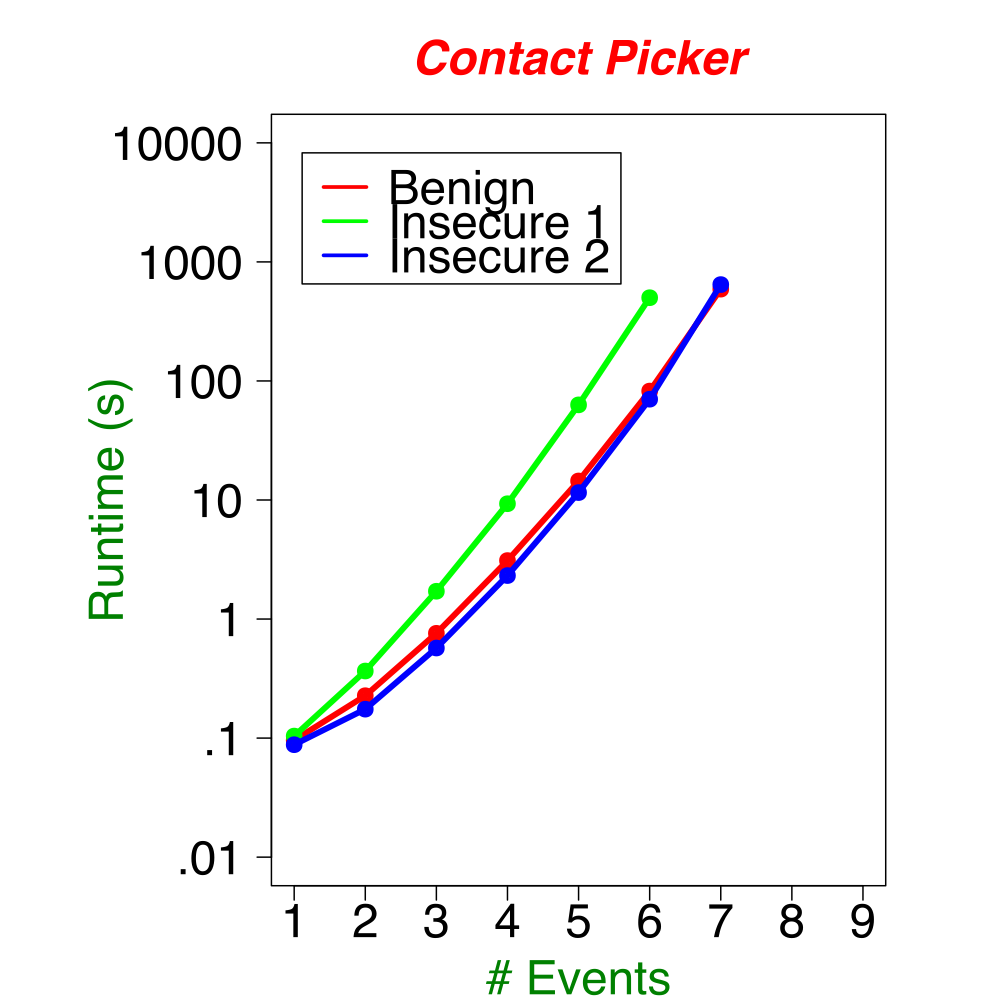
\includegraphics[width=.45\textwidth]{expressive-declassification/contactpicker} &
    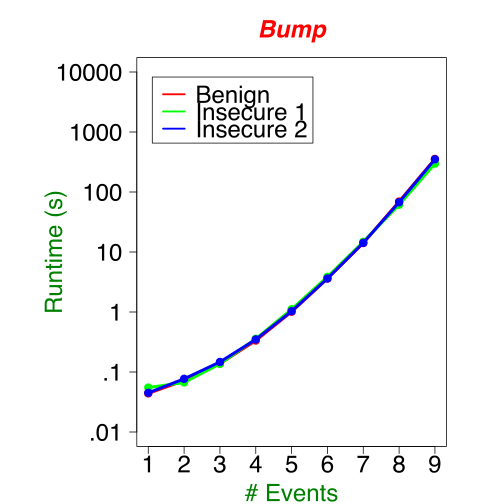
\includegraphics[width=.45\textwidth]{expressive-declassification/bump} \\

    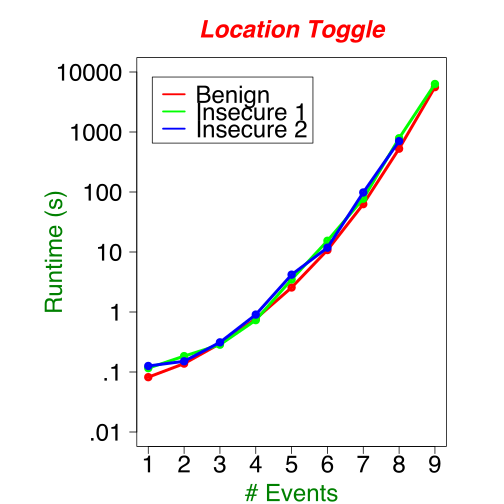
\includegraphics[width=.45\textwidth]{expressive-declassification/locationtoggle} &
    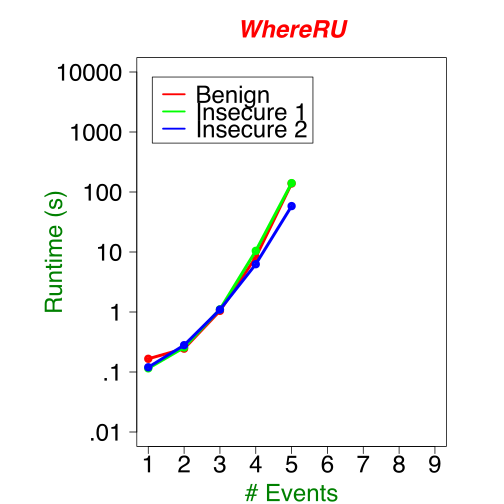
\includegraphics[width=.45\textwidth]{expressive-declassification/whereru}
  \end{tabular}
  \caption{Runtime vs. number of events.}
  \label{fig:performance-graphs}
\end{figure}

In our first set of experiments, we measured how
\toolname{}'s performance varies with input
depth. Figure~\ref{fig:performance-graphs} shows running time (log scale)
versus input depth for all programs and variants.
For each app, we ran to the highest input depth that completed in
one hour.

For each app, we see that running time
grows exponentially, as expected. The maximum input depth
before timeout (i.e., where each curve ends) ranges from five to
nine. The differences have to do with the number of possible events at
each input point. For example, WhereRU has seven possible input events, so
it has the largest possible ``fan out'' and times out with an input
depth of five. In contrast, Bump and Location Toggle have just three
input events and time out with an input depth of nine. Notice also the first
insecure variant of Contact Picker times out after fewer events than
the other variants. Investigating further, this occurs due to
that app's implicit flow (recall the app branches on the value of a
secret input). Implicit flows cause symbolic execution to take
additional branches depending on the (symbolic) secret value.

\paragraph*{Minimum Input Depth.}

\begin{figure*}[t]
  \centering
  \begin{tabular}{ | l | r | r | r | r | r | }
    \hline
    &Input&\multicolumn{3}{c|}{Time (ms)} \\ \cline{3-5}
    App & Depth & Exploration & Analysis & Total \\ \hline
    \hline
    Bump & 3 & 114 &  15 & 142 \\
    Bump (insecure 1) & 5 & 2,100 & 1,577 & 3,690 \\
    Bump (insecure 2) & 4 & 266 & 70 & 344 \\\hline
    Location toggle & 2 &  113 & 12 & 128 \\
    Location toggle (insecure 1) & 2 &  143 & 12 & 163 \\
    Location toggle (insecure 2) & 3 & 117 & 12 & 143 \\\hline
    Contact picker & 2 &  79 & 2 & 94 \\
    Contact picker (insecure 1) & 2 &  325 & 27 & 361 \\
    Contact picker (insecure 2) & 2 &  149 & 9 & 170 \\\hline
    WhereRU & 3 & 849 & 183 & 1,045 \\
    WhereRU (insecure 1) & 3 & 860 & 234 & 1,108 \\
    WhereRU (insecure 2) & 2 & 257 & 10 & 280 \\
    \hline
  \end{tabular}
  \caption{Results at minimum input depth.}
  \label{fig:results}
\end{figure*}

Next, for each variant, we manually
calculated a \emph{minimum} input depth guaranteed
to find a policy violation.
To do so, first we determined possible app GUI states.
For example, in Bump (Fig.~\ref{fig:app-bump}), there is a state with \code{idBox} and
\code{phBox} both checked, a state with just \code{idBox} checked,
etc. Then we examined the policy and recognized that certain input
sequences lead to equivalent states modulo the policy.  For example,
input sequences that click \code{idBox} an even number of times and
then click send are all equivalent. Full analysis reveals that an
input depth of three (which allows the checkboxes to be set any
possible way followed by a button click) is
sufficient to reach all possible states for this policy. We performed
similar analysis on other apps and variants.

Fig.~\ref{fig:results} summarizes the results of running with
the minimum input depth for each variant, with the depths listed in
the second column.
We confirmed that, when run with this input depth, \toolname{}
correctly reports the benign app variants as secure and the other app
variants as insecure.
%
The remaining columns of Fig.~\ref{fig:results} report \toolname{}'s
running time (in milliseconds), broken down by the
exploration phase (where SymDroid generates the set of symbolic
traces) and the analysis phase (where SymDroid forms equations about
this set and checks them using Z3).  Looking at the breakdown between
exploration and analysis, we see that the former dominates the running
time, i.e., most of the time is spent simply exploring program
executions.  We see the total running time is typically around a
second or less, while for the first insecure variant of Bump it is
closer to 4 seconds, since it uses the highest input depth.

Our results show that while \toolname{} indeed scales exponentially,
to actually find security policy violations we need only run it with a
low input depth, which takes only a small amount of time.

\section{Limitations and Future Work}

There are several limitations of \toolname{} we plan to address
in future work.

Thus far we have applied \toolname{} to a set of small apps that we
developed. There are two main engineering challenges in applying
\toolname{} to other apps. First, our
model of Android (Section~\ref{sec:driver}) only includes part of the
framework. To run on other apps, it will need to be expanded
with more Android APIs. 
Second, we speculate
that larger apps may require longer input depths to go from app launch
to interfering outputs. In these cases, we may be able to start
symbolic execution ``in the middle'' of an app (e.g., as in the
work of Ma et al. \cite{Ma:2011}) to skip uninteresting
prefixes of input events.

\toolname{} also has several limitations related to its policy
language. First, \toolname{} policies are fairly low level. Complex
policies---e.g., in which clicking a certain button releases
multiple pieces of information---can be expressed, but are not very
concise. We expect as we gain more experience writing \toolname{}
policies, we will discover useful idioms that should be incorporated
into the policy language.  Similarly, situations where several
methods in sequence operate on and send information should be
supported.  Second, currently \toolname{} assumes there
is a single adversary who watches \code{netout}. It should be
straightforward to generalize to multiple output channels and multiple
observers, e.g., to model inter-app communication.  Third, we do not
consider deception by apps, e.g., we assume the policy writer knows
whether the \code{sendBtn} is labeled appropriately as ``send'' rather
than as ``exit.'' We leave looking for such deceptive practices to
future work.

Finally, since \toolname{} explores a limited number of program paths
it is not sound, i.e., it cannot guarantee the absence of policy
violations in general. However, in our experiments we were able to
manually analyze apps to show that exploration up to a certain input
depth was sufficient for particular apps, and we plan to investigate
generalizing this technique in future work.

\section{Related Work}
\label{sec:related-work}

\toolname is the first system to enforce extensional declassification policies 
in Android apps.  It builds on a rich history of research in usable security,
information flow, and declassification.

One of the key ideas in \toolname is that GUI interactions indicate the 
security desires of users.
Roesner et al.~\cite{Roesner:12} similarly propose \emph{access control gadgets}
(ACGs), which are GUI elements that, when users interact with them,
grant permissions. 
Thus, ACGs and \toolname both aim to better align 
security with usability~\cite{Yee:04}.
\toolname addresses secure information flow, especially propagation of
information after its release, whereas ACGs address only access control.

\paragraph*{Android-based systems.}

TaintDroid~\cite{Enck:10} is a run-time information-flow tracking system
for Android.  It monitors the usage of sensitive information and detects
when that information is sent over insecure channels.
Unlike \toolname{},
TaintDroid does not detect implicit flows.

AppIntent~\cite{Yang:2013} uses symbolic execution to derive the \emph{context},
meaning inputs and GUI interactions, that causes sensitive information to be
released in an Android app. A human analyst examines that context and makes an
expert judgment as to whether the release is a security violation.  
\toolname instead uses human-written LTL formulae to specify whether 
declassifications are permitted. It is unclear from~\cite{Yang:2013} whether AppIntent detects
implicit flows.

Pegasus~\cite{Chen:13} combines static analysis, model checking,
and run-time monitoring to check whether an app uses API
calls and privileges consistently with users' expectations.
Those expectations are expressed using LTL formulae, similarly to \toolname.
Pegasus synthesizes
a kind of automaton called a \emph{permission event graph} from the
app's bytecode then checks whether that automaton is a model for the formulae.
Unlike \toolname, Pegasus does not address information flow.

Jia et al.~\cite{Jia:13} present a system, inspired by Flume~\cite{Krohn:2007},
for run-time enforcement of information flow policies at the granularity of 
Android components and apps.  Their system allows
components and apps to perform trust declassification according to 
capabilities granted to them in security labels.  In contrast,
\toolname reasons about declassification in terms of user
interactions.

\paragraph*{Security type systems}

Security type systems \cite{Volpano:1996} statically disallow programs
that would leak information. O'Neill et al.~\cite{O'Neill:2006} and
Clark and Hunt~\cite{Clark:09} define interactive variants of
noninterference and present security type systems that are sound with
respect to these definitions.

Integrating declassification with security type systems has been the
focus of much research.  Chong and Myers~\cite{Chong:04} introduce
\emph{declassification policies} that conditionally downgrade security labels.
Their policies use classical propositional logic for the conditions.  
\toolname can be seen as providing a more expressive language for
conditions by using LTL to express formulae over events.  
%
SIF (Servlet Information Flow)~\cite{Chong:07} is a framework for
building Java servlets with information-flow control.  Information
managed by the servlet is annotated in the source code with security
labels, and the compiler ensures that information propagates in ways
that are consistent with those labels.  The SIF compiler is based on
Jif \cite{Myers:1999}, an information-flow variant of Java.

All of these systems require adding type annotations to terms in the
program code, e.g., method parameters, etc. In contrast, \toolname{}
policies are described in terms of app inputs and
outputs.

\paragraph*{Event Based Models and Declassification}

Vaughan and Chong~\cite{Vaughan:2011} define expressive declassification policies that
allow functions of secret information to be released after events occur, and
extend the Jif compiler to infer events.  \toolname instead 
ties events to user interactions.

Rafnsson et al.~\cite{Rafnsson:12} investigate models, definitions, and enforcement
techniques for secure information flow in interactive programs in a
purely theoretical setting.
%
Sabelfeld and Sands~\cite{Sabelfeld:2009} survey approaches to
secure declassification in a language-based setting.  \toolname
can be seen as addressing their ``what'' and ``when'' axes of
declassification goals:  users of Android apps interact with the GUI
to control when information may be released, and the GUI is responsible
for conveying to the user what information will be released.

\section{Conclusion}
\label{sec:conclusion}

We introduced interaction-based declassification policies, which describe
\emph{what} and \emph{when} information can flow. Policies are defined
using LTL formulae describing event traces, where events include GUI
actions, secret inputs, and network sends. We formalized our policies
using a trace-based model of apps based on security relevant events.
Finally, we described \toolname{}, which uses symbolic
execution to check interaction-based declassification policies on Android, and
showed that \toolname{} correctly enforces policies on four apps,
with one secure and two insecure variants each.


\renewcommand{\thechapter}{4}

\chapter{User Interactions and Permission Use on Android}

Our last chapter introduced interaction-based declassification
policies. However, it is unclear whether this matches user intuition
about how apps behave. In this chapter, I introduce a system for
studying how permission uses relate to user interaction within
apps. This system, named \apptracer{}, builds on the logging
facilities present in Redexer. It leverages logging and visualization
to help perform an app study over 150 top apps from the Google Play
store. I then follow this up with a 961-participant user study to
investigate how users understand permissions as they relate to the
UI. I found that the app's UI does deeply inform a user's expectation
that a permission will be used, but that the current implementation of
the Android permission system may mislead users under certain
circumstances.

\section{Introduction}

Android has a \emph{permission system} that asks users for
authorization before an app uses sensitive resources such as
contacts or GPS location.
% Older versions of Android asks users to approve a list of app
% permissions at install time, and Android~M improves on this with
% dialog boxes to request authorization at run time before the first
% use. However,
A key challenge in such authorization systems is balancing
user interruptions with making sensitive resource use transparent.
% Currently, Android uses either install-time lists of permissions or
% run-time dialog boxes to request authorization.
We hypothesize that Android's existing authorization systems
(install-time permission lists or run-time dialog boxes, depending
on the version) could achieve a better balance by integrating with the
app's user interface (UI), because the UI deeply informs the user's
mental model of the app's behavior, including security-relevant behavior.
%  If true, then Android's authorization
% system could use the UI to better balance user interruptions with
% making sensitive resource use transparent.

In particular, in this chapter we ask whether \emph{user
  interactions}---button clicks, page changes, dialog boxes,
etc.---can be taken as evidence of authorization to use certain
sensitive resources. If so, this could reduce the need for separate
authorization requests. Conversely, I ask whether sensitive resource
use without an associated interaction suggests a need for additional
authorization requests.
Note that while our studies are heavily influenced by Android, I believe the
results will generalize to related mobile OS's and
similar settings like web apps.

To answer these questions, I conducted two related studies. First, I
(and another grad studnet) reviewed 150 popular Android apps to
determine whether sensitive resource uses are related to user
interactions in existing apps.  If so, an authorization mechanism
integrated with the UI could work well with existing app designs.  To
carry out this study, we developed \apptracer{}, a dynamic analysis
tool that instruments Android apps to log UI actions and resource
uses, and then visualizes the logs as graphs that show temporal
ordering of logged events.
%\apptracer{} then visualizes such logs as graphs, where
%the nodes are UI actions or resource uses, and edges indicate temporal
%ordering. For example, a ``click'' node with an edge to a ``contacts''
%node indicates the users' contacts were accessed immediately after a
%click. 
We used \apptracer{} to determine whether each observed
resource use in each app was \emph{interactive}, meaning either it was
immediately preceded by a related UI event (e.g., accessing contacts
after clicking a button marked ``contacts''), or it was the main focus of
the current screen (e.g., using location on a map screen). 

We found that, across our subject apps, several resources (microphone,
camera, external storage, and calendar) are used almost exclusively
interactively; several others (including bluetooth and phone state)
are used mostly non-interactively (which we call in the
\emph{background} even if the app itself is on screen); and several
resources (most notably contacts and location) exhibit a mix of
interactive and background uses. These results suggest interactive and
background uses may call for different authorization mechanisms, and
that these mechanisms cannot necessarily be divided strictly by
resource.

% \jeff{loc is actually used interactively 40\% of the time, so I wonder
%   if it's really a good representative of that last category?}

These results informed the design of our second study, a
961-participant online survey investigating participants' expectations
about interactive and background permission uses. Each participant
viewed a slideshow of two usage scenarios for a mock mobile app, where
each scenario shows a short interaction (e.g., launching the app,
clicking a button, etc.) and then asks if the participant expects
microphone, location, and/or contacts to be used after the
interaction. We chose these resources to reflect a range of
interactivity as measured in our app study.  We aimed to gain insight
into how different factors
%(the resource and app being used and the type of interaction)
affect user expectations, and therefore which authorization mechanisms
might be appropriate for different usage patterns.
%
%In particular, we studied three hypotheses: whether users
%are likely to expect resources to be accessed after an interaction
%such as a button click; whether users expect background accesses of
%resources that are very common in apps; and whether users expect a
%resource to be accessed again if it was accessed before within an app.
%\jeff{Do we need prev?}

%In our study, we showed each participant a slideshow describing a
%typical usage scenario for one of two mocked mobile apps,
%\emph{HealthyFit Tracker} and \emph{FindMeCoffee}. Each scenario
%includes a pair of trials, where each trial shows a short interaction
%with the app (e.g., launching the app, clicking a button, etc) and
%then asks the participant whether they expect microphone, location,
%and contacts to be used after the interaction.

As we anticipated, we found that users are much more likely to expect 
resources to be accessed after a related interaction than in the 
background. However, we also found that seeing one 
interactive use does not prime the user to expect a future 
background use, indicating a potential weakness in the Android~M request-on-first-use 
authorization model. In contrast, our findings show that an 
authorization request at launch does increase expectations for 
both interactive and background accesses, perhaps because it better conveys the idea that 
the resource could be accessed at any time.

%an authorization request at launch does 
%increase expectations for later accesses. This has implications 
%for the Android~M permissions model's app
%users do not expect a background use if the previous use was an
%interactive use, but expectation does increase if authorization was
%requested when the app was launched.  Finally, we found users did not
%necessarily expect commonly used resources to be used in the
%background. \jeff{Do we want to give numbers for the above?}

Drawing on the results of our studies, we make three design 
recommendations. First, resource uses should be made after associated 
interactions as much as possible. Given the current makeup of apps, this 
should be achievable for many commonly used resources without extensive 
effort. Second, separate authorization dialogs might be unnecessary
for resources that are accessed mostly interactively (see, e.g.,~\cite{Roesner:2012}). 
Finally, authorization for background resource uses should be distinct 
from authorization for interactive uses, and these background authorizations 
may be most effective when the app is launched. 

%\kris{Mike said that we didn't point out that we were really defining
%  a new notion of context for these apps, more informed by the
%  implementation, and that that might lead us to be more plausibly
%  enforced via some security mechanism.}

% We found that users' expectation of resource use increased as they were
% shown more interactive access pattern.  Specifically, showing our participants
% a button click had the largest effect on their likeliness to expect a resource 
% use, more so than the impact of presenting an authorization request.  We 
% also observed that the relationship between real-world frequency and expectation
% was not consistent across all apps.  Our participants were likely to expect location 
% to be accessed frequently in the background and the microphone to be rarely 
% used outside of very interactive cases, which matched the results of our app 
% study. However, users did not expect their contacts to be accessed, which
% contradicts our previous findings.  Finally, we found that users are more likely 
% to expect a resource use in the background if they have previously seen an 
% indication of some background usage, such as a pop up notification indicating 
% that they are ``near a coffee shop'' which indicates the app accessed the user's
% location.  However, they were not more likely to expect a background use if 
% they were previously shown an interactive access even if an resource 
% authorization was presented on the first use.

% Based on the results of our studies, we observe that Android is
% already moving toward contextual security, and we recommend continuing
% in this direction. We found that many apps are already constructed so
% that, for very sensitive resources such as the microphone, access is
% already contextual in nature. Changing apps fit to this paradigm for most 
% resources would align apps with users' expectations.  Additionally, due to
% level of expectation we observed associated with highly contextual accesses, 
% authorization requests on interactive accesses would no longer be necessary.
% We also recommend more explicit authorization of background use as users 
% did not appear to be aware of all background resource accesses.

% meaning in a context with a clear UI action such as a button click. We
% also found that when resources are used in the background, it is
% typically to support foreground behavior, e.g., loading contacts
% asynchronously.  Finally, we found that location and phone identifiers
% (e.g., IMEI) are often used in the background and without notifying
% the user, typically to support advertising.  

% We also observed that apps only notified the user of a resource access
% when required to do so by Android M.  The vast majority of apps
% presented authorization requests directly before the first resource
% use and a few included a brief description for why they accessed the
% resource just before the standard Android M authorization dialog.  We
% used our observations to inform the construction of our user study.

% the log---was it after a button click, a page change, at app startup,
% in the background, or uncertain; and was there any authorization request,
% such as a modal dialog box with an alert message,
% prior to the use. %\jeff{What kinds of notifications were there?}

% Despite these changes, we observe that by not considering the user
% interface, Android's authorization approach
%  This paper aims to shed light on this hypothesis with two
% complementary studies. First, we ask the question, \emph{do existing
%   apps users permissions in an interactive manner?}, meaning, is it
% the case that there is typically a clear connection between user
% interactions with an app and access to sensitive resources. We
% partially answer this question by applying a dynamic analysis to 150 top apps
% from Google Play to determine 

% One advantage of the Android~M model is that it may allow users to
% better consider the
% \emph{context}~\cite{Nissenbaum:2004,Wijesekera:2015} before granting
% permission to an app.\footnote{There are also many other advantages to
%   the Android~M model, most notably allowing users to enable and
%   disable app permissions even after the app is installed.}  

% These are difficult questions to answer, and in this paper 
% In this paper, we conduct two complementary studies exploring how the
% context defined by user interactions---what window is on the screen,
% what buttons have been clicked, etc.---relate to actual and expected
% permission uses on Android. We measure actual permission uses in
% existing apps by analyzing the results of a dynamic program analysis.
% We measure expectations via a user survey.

% Mobile operating systems such as Android and iOS use permissions to
% protect access to sensitive resources including user data (e.g.,
% contacts) and device capabilities (e.g., GPS location). While
% permissions are conceptually simple, they suffer from a key
% limitation: once a permission to access a resource is granted, the app
% can access that resource for any purpose, at any time, unless and
% until the permission is manually revoked. Thus, apps that are
% legitimately granted permission for one purpose might misuse it for
% another.
%\jeff{add cites}.

% A potential remedy to this situation is to also consider the
% \emph{context}~\cite{Nissenbaum:2004,Wijesekera:2015} before allowing
% sensitive resource accesses. While contextual security has been
% considered before for mobile
% devices~\cite{Chen:13,Wijesekera:2015,Roesner:2012}, prior work uses
% shallow notions of context (e.g., is the app in the foreground or
% background) or focuses on how mobile operating systems or apps could
% be modified to better support context
% \cite{Roesner:2012,Roesner:2013,Ringer:2016}.

% Combining the results of these studies we identify a middle ground
% within the Android permissions landscape, wherein permission should be
% requested on each \emph{new} use of the permission. We call this
% pattern-based-access-control (PBAC). We found that pattern based
% access control could likely be used for almost all apps using
% microphone and video, and nearly all uses of contacts and external
% storage. For example, although a user may be fine with their contacts
% being accessed after clicking a button, they may not be comfortable
% with the same behavior happening each time the app runs. PBAC
% separates these two policies, and attempts to ask users about resource
% access in a minimally invasive way that still controls for their
% expectations.


% In this paper, we survey the context of resources uses in 150 top
% apps, and compare that to user expectations gathered in a
% medium-scale user study.  To perform our app study we developed
% \apptracer{}, a dynamic analysis tool that allows us to visualize app
% logs and understand where resources are used with respect to the app's
% UI. We used \apptracer{} to assign codes to each app corresponding to
% the set of resource access patterns we identified.

% Our user study attempts to understand whether the resource usage
% patterns apps use aligns with user expectations. We show users
% slideshows of app traces, testing various combinations of relevant
% events (such as pressing a ``find coffee'' button) and ask what
% resources they expect will be used. We test a variety of times (on app
% launch, after first use, never) at which users are presented with
% dialogs showing resources will be accessed. We test this for three
% resources (location, microphone, and contacts), and a variety of
% permutations of app scenarios.

% We set up our study to test the efficacy of the Android M (just in
% time) permissions model. It is well known \cite{Felt:2012soups} that
% install-time permissions are frequently ignored, but we posited that
% there may be some circumstances where no dialog was necessary because
% it was clear from context (e.g., contacts accessed after clicking on an ``add contact''
% button). We also posited that there may be circumstances under which a
% user is fine with authorizing some resource accesses, but then later
% wishes to revoke that access.

% Our app study identifies that some resources (such as microphone and camera)
% are almost exclusively used in an interactive way within top
% apps. Based on these results, we recommend that access use for these
% resources be tied to clearly identifiable UI elements, and other uses
% should be seen as suspicious. We identified another class of resources
% (contacts and external storage) which are frequently accessed in an
% interactive way, but for programmatic reasons may be accessed at a
% different time than a specific interaction. For example, an app may
% pre-fetch a list of contacts to be shown to the user later. Last, we
% found that some resources such as phone information (e.g., number and
% unique ID), location, and user accounts are frequently accessed
% without the user's knowledge. Based on the results of our user study,
% we found that these resources were less sensitive than others, but
% believe users should still be educated as to their collection.

% Combining the results of these studies we identify a middle ground
% within the Android permissions landscape, wherein permission should be
% requested on each \emph{new} use of the permission. We call this
% pattern-based-access-control (PBAC). We found that pattern based
% access control could likely be used for almost all apps using
% microphone and video, and nearly all uses of contacts and external
% storage. For example, although a user may be fine with their contacts
% being accessed after clicking a button, they may not be comfortable
% with the same behavior happening each time the app runs. PBAC
% separates these two policies, and attempts to ask users about resource
% access in a minimally invasive way that still controls for their
% expectations.

In earlier versions of Android, users were presented
with a list of permissions requested by an app at install time. The
user could then either grant the app full use of those permissions or
not install the app at all. This model had a number of
problems: few users comprehended or even read the list of permissions~\cite{Felt:2012soups},
and many apps requested more permissions than they used~\cite{Felt:2011}. 
Because of these
issues, Android M~\cite{AndroidMPermissions} switched to a model where
apps ask for a permission the first time it is needed; the permission is 
then granted indefinitely.
%%  This
%% brings Android closer to enforcing \emph{contextual
%%   integrity}~\cite{Nissenbaum:2004}, which states that resources
%% should be accessed in accordance with contextual norms.  
%However,
%on Android M, permissions are still granted indefinitely.

In our work, we ask whether authorization systems similar to
Android's can be improved by taking the user interface into account.
% In this paper, we study foundational questions about
% whether existing apps use permissions in a contextual manner
% (shedding light on whether asking for permission on the first use is
% necessary or sufficient); whether users expect permissions to be used
% contextually; and whether user expectations and current practice
% align. 
Note that our work is orthogonal to the question of whether
permissions are at the right level of granularity
\cite{jsjeon:spsm12,Bugiel:2013} or protect the right
resources~\cite{Felt:2012spsm}.

% Android security---particularly the permission system---has been
% heavily studied in the research community
% \cite{Felt:2011,Felt:2012spsm,Sarma:2012,Wang:2013,Chia:2012,Liu:2016,Balebako:2013,Fu:2014}
% (among many others). There is also substantial work
% \cite{Wijesekera:2015,Thompson:2013,Jung:2012} indicating that users'
% expectations about resource accesses depend on the context.

% Our paper builds on the prior work by studying the extent to which
% existing \cite{Ringer:2016,Micinski:2015,Yang:2013,Roesner:2012,Roesner:2013,Chen:13} contextual security systems could be applied to
% existing apps. Our paper also studies how app UI context influences
% user expectations about resource usage. We are unaware of other
% existing work that tries to answer these questions with similar
% studies. \jeff{Not sure how to word this.}

\paragraph*{Contextual Security on Mobile Devices}
%
% It has been repeatedly shown
% \cite{Thompson:2013,Jung:2012,Almuhimedi:2015,Balebako:2013,Fu:2014}
% that users are frequently surprised by resource accesses that happen
% while apps are in the background. For example,
%
The motivation for our work, that authorization can be better
integrated with the UI, exemplifies \emph{contextual
  security}~\cite{Nissenbaum:2004}, which suggests security decisions
should take the context into account. Several researchers have
studied contextual security on mobile devices. Almuhimedi
et. al~\cite{Almuhimedi:2015} showed users historical data about how
apps accessed their locations. They found 95\% of users reassessed the
apps' need for location, with 58\% of those users further restricting
location access.  King~\cite{King:2012} found users
are more likely to expect sensitive resource accesses when
suggested by the context. Felt et. 
al~\cite{Felt:2012hotsec} proposed a process for deciding the 
appropriate authorization mechanism for a permission based on the a
permissions' use in context. Several
researchers~\cite{Balebako:2013,Fu:2014,Wijesekera:2015} found users
are surprised by some sensitive resource accesses
%, such as location
%and phone information,
that occur when apps are in the
background. Most closely related to this paper, in a field study 
Wijesekera et al.~\cite{Wijesekera:2015} found that context is an
important factor in determining expectation of resource use.
Our work builds on this finding by using a controlled experiment 
to distinguish how different contextual factors, including consecutive 
interactions, contribute to user expectations.

The works just mentioned mainly define context as whether the
app is on or off the screen. In contrast, we use a
much richer notion of context based on sequences of UI actions. 

%While Wijesekera et. al~\cite{Wijesekera:2015} do perform
%a field study on a set of users and determine that context is an
%important factor in determining expectation of resource use, our work
%performs a controlled experiment across a variety of different
%variables. Specifically, our definition of app context is guided by a
%deeper notion of the sequence of actions a user took through an app
%(e.g., the sequence of clicks) whereas theirs only considers whether
%the app was on the screen at the time (and provides users a screenshot
%at that time to make decisions about if an access is expected). This
%also allows our study to reason about sequences of accesses and
%compare expectation about future access based on the expectation of
%the prior, incorporating aspects of the newer (Android M) architecture
%present in apps since that work took place.



% Wijesekera
% et. al~\cite{Wijesekera:2015} explored contextual integrity on Android
% and found that many users were surprised by some sensitive resource
% accesses that occur when Android apps are in the background. Flu
% et. al~\cite{Fu:2014} used run-time disclosures to show users which
% apps accessed their location. Many users were surprised to learn apps
% they did not frequently use accessed their location in the background.
% Balebako et. al~\cite{Balebako:2013} created the ``Privacy Leaks''
% tool, which allows users to audit which apps use their information in
% real time. They similarly found users were surprised that apps access
% location and phone information even when the apps had not been used
% much.



%  includes whether the app is in the background, but also recent
% actions in the app's UI.  Our paper complements the above studies by
% showing how an app's UI influences user expectations about resource
% usage.

\paragraph*{Enforcing Contextual Security}
Many systems have been proposed to enforce contextual security in
apps.  Chen et. al~\cite{Chen:13} present Pegasus, a static analysis
system for analyzing apps and enforcing policies based on
\emph{permission event graphs} (PEGs). For example, Pegasus can check
that contacts are only accessed after clicking a certain
button. PEGs inspired the design of \apptracer{}. However, \apptracer{}
uses dynamic (rather than static) analysis to reduce issues of false
positives---every behavior \apptracer{} logs occurred in an actual run,
whereas static analysis may report sensitive resource accesses that can never actually occur.
%conservatively overestimates the runtime
%behavior of the program (for example, it ).

% However, Permissions Event Graphs take into account a deeper knowledge
% of the Android API. \apptracer{}'s graph merely orders events
% temporally, with only a portion of edges coming from Android's
% semantics. This means \apptracer{} is less precise at understanding the
% program's behavior, but allows us to scale up to all of the Android
% API.

Yang et al.~\cite{Yang:2013} presented AppIntent, which uses symbolic
execution to determine sequences of UI events that lead to information
leakage. Micinski et. al~\cite{Micinski:2015} use symbolic execution
to enforce secure information-flow properties based on UI
events. While both systems are promising, in practice symbolic
execution is difficult to run at scale on Android apps due to the
complexity of modeling the Android framework.

Stiegler et al. developed CapDesk~\cite{capdesk} and later Polaris~\cite{Stiegler:2006}, 
two capability-based desktop system that utilize user interaction to drive access control.
However, CapDesk and Polaris's focus is limited to file access.
Roesner et. al~\cite{Roesner:2012} expand user-driven access control with \emph{Access Control
  Gadgets} (ACGs), which tie resource accesses to certain UI elements,
e.g., an ACG might allow location to be used only after a specific
button is clicked. ACGs were later expanded to work on Android, with 
and later without modifying the operating system~\cite{Roesner:2013,Ringer:2016}.
The original ACG paper includes a user study measuring 
expectations related to interactive permission uses; our work 
expands on this idea to study a broader variety of factors and 
use cases. 
%work on Android \cite{Roesner:2013} by modifying the Android runtime.
%Recent follow up work by Ringer et. al~\cite{Ringer:2016} allows ACGs
%to be used on an unmodified operating system. 
While the current paper
does not directly implement or measure ACGs, our findings do support
the use of ACGs.
% While our user study incorporates elements of the study
%done in the original paper on ACGs---specifically, we also measure
%expectation change as the result of clicks---we also measure user
%expectation across a larger possible design space encompassing
%different user actions and subsequent accesses.

\section{App Measurement Survey Methodology}

\begin{figure}[tb]
  \centering
  \includegraphics[width=.7\columnwidth]{leakfinder-chi2017/img/app-study-diagram.png}
  \caption{App Measurement Survey Procedure.}
  \label{fig:measurement-summary}
\end{figure}


In our first study, we reviewed a set of popular Android apps to determine
how UI actions and resource uses are related.
Figure~\ref{fig:measurement-summary} gives a high-level
overview of our review process, which ultimately produces
%  which uses \apptracer{}, a dynamic
% analysis and visualization tool we developed to show an app's UI
% events and permission uses.  Since
% \apptracer{}'s visualization is complex, two coders reviewed each
% visualization separately and then came to agreement for every app. The
%final result is
a set of \emph{resource use codes} that indicate, for each resource use,
what event (if any) caused the use. For example, we might
determine that in some app, contacts were accessed just after a button
click, or location was used immediately when the app launched.

The next subsections walk through the review process in detail.

% We wanted to understand and categorize the ways in which typical apps
% access users' resources. To do this, we surveyed 150 apps using a tool
% we built to help visualize the connection between UI interaction and
% use of sensitive resources. Using this tool, we applied an iterative
% manual-coding process to identify the set of resource-access patterns
% present in each app. Figure~\ref{fig:measurement-summary} shows a
% high-level overview of our process. In the following subsections, we
% provide details about the design and operation of our visualization
% tool, as well as our manual coding process.

\subsection{Binary Rewriting and Execution Logging}

The first step of our process uses \apptracer{}, a dynamic analysis tool
we developed. \apptracer{}
instruments the subject app so that, when run, it writes
a log of UI events and permission uses. \apptracer{} adds
instrumentation using Redexer~\cite{jsjeon:spsm12}, a
rewriting tool for Dalvik bytecode (the language
to which Android apps are compiled). Generally speaking, \apptracer{}
instruments code by appending a \code{log} method to the bytecode and
inserting calls to \code{log} at the beginning of UI-related callbacks
(e.g., \code{onClick} handlers for button events) and just before
calls to permission-protected methods (e.g., \code{getLastLocation}).

We identified methods associated with the UI using the Android
documentation. We identified permission-protected methods using the 
PScout dataset~\cite{Au:2012}, which attempts to list every
security-sensitive method and its associated permission. PScout also
includes information about sensitive content providers, intents, etc.
%
Note that while PScout is reasonably thorough, we found several cases
it missed. For example, we observed several visual
indicators of SD card use that had no corresponding log entry
\apptracer{}.  After
investigating the apps' decompiled code, we found the SD card was used
via Java IO methods omitted by PSCout. Whenever we found
such cases, we added the missing methods to our copy of the PScout
database and reran our evaluated apps.

% For example, we noted that PScout did not include methods in the
% popular Google Play Services API.

Once an app has been instrumented, a tester runs it to generate a log.
(Note that one log is usually sufficient because in most apps, any app
state is reachable from any other app state.)  We elide
the details of the log, but at a high level, for
each UI event, \apptracer{} records the type of event and the corresponding
parameters (e.g., what button was clicked, which menu option was
selected, etc.). For each permission use, \apptracer{} logs the name of
the called method and its arguments.

\subsection{Log Visualization}

\begin{figure}[tb]
  \centering
  \begin{subfigure}{.25\textwidth}
    \includegraphics[width=\textwidth]{leakfinder-chi2017/img/click.png}
      \vspace{-.3in}
      \caption{Click}
      \label{fig:click}
  \end{subfigure}
  \begin{subfigure}{.25\textwidth}
    \vspace{-.1in}
    \includegraphics[width=\textwidth]{leakfinder-chi2017/img/uncertain.png}
    \vspace{-.3in}
    \caption{Uncertain}
    \label{fig:uncertain}
  \end{subfigure}

  \begin{subfigure}{.25\textwidth}
    \includegraphics[width=\textwidth]{leakfinder-chi2017/img/startup.png}
    \vspace{-.3in}
    \caption{Startup}
    \label{fig:startup}
  \end{subfigure}
  \begin{subfigure}{.25\textwidth}
    \vspace{-.1in}
    \includegraphics[width=\textwidth]{leakfinder-chi2017/img/bg-evt.png}
    \vspace{-.3in}
    \caption{Background-External}
    \label{fig:bg-ext}
  \end{subfigure}
  \caption{\apptracer{} graphs and corresponding resource access patterns in our codebook.}
  \label{fig:leakfinder-ex-graph}
\end{figure}

After the tester produces a log, the next step is log visualization.
Figures~\ref{fig:click}--\ref{fig:uncertain} show example
portions of \apptracer{}'s graph-based visualization, redrawn for
compactness and to omit most package names.
Here, light blue boxes represent
\emph{activities}, which are the ``screens'' of the
app. Within each activity, gray ovals represent the beginning
of that activity (``entry,'' which usually corresponds to the
\code{onStart} handler), UI events (e.g.,
``click''), or system events (e.g.,
\code{BATTERY\_CHANGED}).
Red rectangles indicate calls to methods
protected by the named permission. There is an edge from node A to node B if A
occurs immediately before B in the log. For example, in
Figure~\ref{fig:click}, contacts were read immediately after
the \code{ImportContactActivity} activity was started.

Since logs can be quite lengthy, \apptracer{} heuristically merges
nodes that arise from the same position in the bytecode. This
sometimes results in ambiguity. For example, in
Figure~\ref{fig:uncertain}, the single \code{onReceive} node actually
represents calls to an Android broadcast receiver that \apptracer{}
coalesced. We discuss this more below.

%  has been collapsed to
% represent multiple clicks within the activity.
% \kris{\apptracer{} *sometimes* disambiguates based on the resource
% identifier of the click, but not when a click handler is registered
% on multiple different objects, in that case you just check the
% receiver of the click, which we explain vaguely next}

Finally, \apptracer{} also allows the user to directly view the
log file entries corresponding to a node in the graph. This is
useful to retrieve more detailed information about the node. For
example, when reviewing Figure~\ref{fig:click}, we looked in the log
to determine that the clicked button had text associated with contacts.  As
another example, we used the logs to distinguish SD card accesses to
user files from accesses to the app's own storage. We do not count the 
latter as a sensitive resource access because it accesses data owned by 
the app. 
% This feature was 
% also used to determine whether or not reads/writes of the SD 
% card were made to files containing sensitive user information by 
% checking associated file path.  We only generated codes in situations 
% where user files were accessed to avoid over-counting when the app 
% simply saved its own information to the SD card.

\subsection{Resource Uses}

The next step is to examine the \apptracer{} graph and record a set of
codes that accurately categorize various resource accesses.
More precisely, for each red node in the graph, the coder
assigns a pair of the form $(\textit{resource}, \textit{pattern})$,
where \textit{resource} indicates what is protected by the permission
and \textit{pattern} is one of six different UI patterns, discussed
next.

To keep our results understandable, we grouped together resources
according to Google's permission
groups~\cite{permissiongroups}. For example, the single \code{SMS}
resource includes more fine-grained permissions such as \code{READ\_SMS} and
\code{SEND\_SMS}.
%\jeff{Are there additional permissions in SMS?}
%\dan{Yes, there's RECEIVE_SMS, RECEIVE_MMS, and a few others}

% This loss of precision conflates resource access but is
%consistent with current Android permissoin models.
% \apptracer{} does, however, provide us with insight towards each
% fine-grain resource within the permission groups which mitigates
% uncertainty that may arise while investigating apps.

We developed an initial codebook for UI patterns based on our
knowledge of Android app development. We then iteratively applied our
codebook to sets of five apps (not in our evaluation set) at a time
and adjusted the codes as necessary. After evaluating a total of
twenty apps, we felt we had reached a codebook with a minimal set of
orthogonal patterns.

% We arrived at this codebook based on our knowledge of Android app
% development and a preliminary analysis of a small set of apps. We used
% a content analysis based approach, starting with an initial set of
% codes we derived from the patterns we saw \apptracer{} generating and
% the concepts from related literature. We then iteratively applied our
% initial codebook to sets of five apps (not in our evaluation set) at a
% time, eventually evaluating twenty apps. We removed or regrouped
% redundant codes as appropriate, until we ended up with a codebook
% representing a minimal set of orthogonal patterns we saw in apps.

The six access patterns in our codebook are grouped into three categories.  First 
are the \emph{interactive} patterns \textit{Click} and
\textit{Page}. The code \textit{Click} indicates
resource use preceded by a UI event %interaction
 (including non-clicks such 
as swipes). For example, in Figure~\ref{fig:click}, we coded
\code{READ\_CONTACTS} as \textit{Click} because the contacts were
accessed on a straight-line path from the click of a button labeled as importing
contacts.
 \textit{Page} codes uses that are clearly associated with an activity
 but are not associated with exactly one
click.  For example, \emph{Page} would code the use of
  location during an activity that shows a
list of nearby stores.

Second, in the \emph{background} patterns \emph{Startup},
\emph{Bg-App}, and \emph{Bg-Ext}, the resource use has no obviously
connected user action. %interaction.
 \emph{Startup} codes a resource accessed
 right after app launch but before any screen appears
 (and is thus disjoint from \emph{Page}), e.g., the use of accounts in
Figure~\ref{fig:startup}, which occurs in a thread created at app
launch. \emph{Bg-App} codes a resource used while the app is
in the foreground, but with no clearly related user action.
%interaction.
 For example, a graph similar to Figure~\ref{fig:click} would be 
 coded as \emph{Bg-App} if a button labeled for importing contacts 
 was followed by the \code{GET\_ACCOUNTS} permission 
 rather than \code{READ\_CONTACTS}.
 \emph{Bg-Ext} denotes a
resource used due to a system event, meaning it would be used 
whether or not the app is on screen. For example, in Figure~\ref{fig:bg-ext},
accounts are read after the \code{BATTERY\_CHANGED} system event.

Finally, \emph{Uncertain} denotes a resource access that did not fit any
of the previous patterns. In Figure~\ref{fig:uncertain}, we see a
path from a system event to \code{onReceive} to \code{READ\_CONTACTS},
which should be coded as \emph{Bg-Ext}. But, the \code{onReceive} node also 
has an incoming edge from the click handler and the back button.
These uses would be coded as \emph{Bg-App}.
(The \emph{Click} and \emph{Page} codes do not apply 
because the associated buttons do not indicate contacts will be used.)
Because there are multiple possibilities, we code this case as \emph{Uncertain}.

If desired, an \apptracer{} user can subsequently review the logs to
try to resolve the 
uncertainty. For example, here the log entry associated with 
\code{BATTERY\_CHANGED} is followed by a call to
\code{onReceive} and then \code{READ\_CONTACTS}. Thus, the permission
use is coded as \emph{Bg-Ext}. We then separately looked at the log
entries for \code{click} and \code{back\_button}, and found they
were followed by an \code{onReceive} that was \emph{not} followed by
\code{READ\_CONTACTS}. Thus, examining the logs allowed us to
distinguish paths that we merged in \apptracer{}.

% Kris: This now sounds right to me. Maybe we should be more explicit
% about beating the reader over the head with this fact: just because
% there's an edge from BATTERY_CHANGED to onReceive, and there's an
% edge from onReceive to Click, and there's an edge from onClick to
% contacts, does *not* necessarily imply there is a transitive edge
% between them. Maybe this is worth pointing out more obviously?

Note that for each app we only count each $(\textit{resource},
\textit{pattern})$ pair once, no matter how often it occurs in the log.
A stronger notion of frequency would be hard to interpret, since it would
depend on how \apptracer{} heuristically coalesces graph nodes as well as 
to how the tester explored the app.
%, rather than indicating, e.g., the 
%frequency of accesses in a typical app execution.

% \subsection{Authorization}
 
% In addition to coding resource uses, we also used \apptracer{} to code
% the \emph{authorization level} for each resource used somewhere in the
% subject app. There are three possible authorization levels. \emph{On
%   First} codes that the app presented the user with a dialog asking
% for authorization at the first use of a resource (and not subsequent
% uses). \emph{On Launch} codes that the app asked for authorization
% once when the app was first launched. \emph{Never} codes that the app
% did not ask for authorization at run time (e.g., it was written for
% earlier versions of Android that asked for authorization at install
% time).

% \textit{Never} if the app did not notify the user of the resource
% access. This is possible in Android M either because the app was
% developed for an earlier API version or the resource is not part of
% one of Android's ``dangerous'' permission
% groups~\cite{dangerousperms}.  For example, if the app accessed the
% user's Bluetooth resource, Android M does not require and
% authorization dialog to be presented to the user.

% For example, if an app accessed location using a callback after the
% ``find coffee'' button was pressed, we assign it the code (Location,
% Click, Continuous). There are also limited cases where \apptracer{} does
% not give us enough information to decide the pattern being used. In
% these cases, we mark the pattern as undecided. We comment below when
% and why this happened and how we might improve \apptracer{}, but note
% that this happened relatively infrequently.

% For example, if an app's only access of location was after the ``find
% coffee'' button was pressed, and no notification was presented to the
% user, then we assign the tuple (Location, Never).

\subsection{Coding Apps and Resolving Differences}

Coding the resource uses of an app is inherently complex. Thus, two
coders reviewed apps independently in sets of 15 and met after
each set to resolve differences.  Coders took
approximately 10--20 minutes to code each app, and resolving
differences for a set of 15 apps took approximately 30 minutes.

Most differences between coders were due to one coder overlooking
a path or a resource in the \apptracer{} graph.
In almost all such cases, when the other coder pointed
out the omission, the first coder would quickly
reach the same conclusion as the other coder.
%
The remaining differences were caused by disagreements about whether
the resource use was interactive. For example, one app read a user's
accounts within an activity for filling a form. One coder
recorded this as \emph{Click}, since the accounts were read after a
click. The other coder recorded this as \emph{Bg-App}, because there
was no observable use of the account data, such as pre-filling the form with 
data from the user's existing accounts. After encountering several such
cases, the coders decided on a general principle of coding uses as
\emph{Bg-App} unless the UI explicitly mentioned that the resource
could be used---hence, this example was resolved as \emph{Bg-App}.

Inter-rater reliability between our coders for the non-visualization-error 
disagreements was Krippendorff's $\alpha=0.897$, indicating close agreement~\cite{kripalpha}.
% to measure the
%inter-rater reliability between our two coders for the non-visualization-error
%disagreements. We reached an $\alpha$ of 0.897, indicating close
%agreement.

%Jeff: I found the following mysterious. How would anyone know what
%the expected disagreement is? I suspect it's better to just say what
%conclusion to draw from the final alpha value rather than try to
%explain how the statistic works.
%using, which calculates the difference between the expected
%disagreement and observed disagreement between reviewers.
 
\subsection{App Selection}

We drew our subject apps from a larger set comprising the 20 top
downloaded free apps\footnote{as of June 11, 2016} from the
27 non-gaming categories on Google Play. We excluded gaming apps
because they typically use native code that \apptracer{} cannot
analyze. This yielded 503 apps (note there is overlap between
categories).

% We used top apps because we expect the behavior in
% those apps represents what users typically see.
% While it is likely that the patterns in these apps does not
% generalize to all apps, we expect that results about user
% expectations of permission usage will apply more generally.

We then randomly selected 150 apps to evaluate, subject to the 
constraint that no more than two apps were from the
same developer. (We wanted to avoid bias due to overrepresentation of
apps coded in the same style.). We excluded any 
apps that could not be run with \apptracer{}, replacing them with 
new randomly drawn apps to maintain an evaluation set of 150. 

We excluded 48 apps because Redexer fails when rewriting them and
\unusableerrors{} apps because either they refuse to run if modified
(due to internal or system signature checks) or they are primarily
implemented in native code. 
%Jeff: The Redexer/apktool difference is probably not important
% We excluded \redexererrors{} apps because Redexer fails
% when rewriting them and \apktoolerrors{} apps because they cannot be
% unpackaged and repackaged by the open source tool
% apktool~\cite{apktool}, which Redexer depends on. 
In most cases, we created accounts when signup was required to fully exercise an app, but we 
excluded \accountserrors{} apps because they require accounts that are hard
to set up online or require a fee (e.g., bank accounts).
%  performs checks that abort if its bytecode was
% rewritten; the app was preinstalled on our test devices \jeff{say what
%   model these are} and hence the modified version couldn't be
% installed due to a signature mismatch; or the app was primarily
% implemented in native code.



% Of the top Android apps, we found that a few developers, such as
% Google and the GO Dev Team, published a significant number of the top
% downloaded apps.  Therefore, We limit our maximum studied apps per
% developer to 2 to ensure that our results are not biased toward the
% set of best practices employed by a small number of companies.

%To get to 150 apps, we skipped \removedapps from our list of apps. We


\subsection{Limitations}

There are several potential limitations to this study. First, the tester
may miss some app behavior, leading to a log that omits
some possible resource uses and contexts. We tried to alleviate
this concern by exercising as much of the app as possible. However, we
did not use app features that required payment.

Second, \apptracer{} has limitations mentioned above: it may miss UI
events or permission-protected methods, and it merges nodes that
correspond to the same position in the bytecode. We tried to address
the former issue by looking for cases where we expected an event to be
in a log but it was not, and then adding the missing events or
methods. We addressed the latter issue by manually disambiguating some
of the uncertain cases.

% kris: We didn't really systematically do this, we just marked these
% cases as ``uncertain.'' Should we instead just say we marked them as
% uncertain, and since there were so few of them it was mostly fine?
% This is how we would resolve this problem if we were looking to use
% this tools to really dig into apps.

Third, our study reviewed only popular Android apps. Observing that a 
resource is already accessed interactively in 
popular apps would indicate that changing the Android framework 
or system to implement interactivity-related protections for those 
accesses may be reasonable. These apps also represent the 
common case and likely help to set user expectations about apps 
and permissions. However, we note that the apps we 
examine likely differ from the long tail of other apps in important ways; 
popular apps are likely implemented to high standards and unlikely to be 
malicious. We leave similar measurements 
on a broader set of apps as future work.

% Kris: better rewording here?

\section{App Measurement Survey Results}

\begin{figure}[t]
\centering % If we use something other than \columnwidth
\includegraphics[width=.6\columnwidth]{leakfinder-chi2017/img/Access_per_Resource_Groups.png}
\caption{Percent of observed patterns of each type, per resource. 
Bar labels indicate how many apps
  we observed using each pattern, non-normalized.}
\label{fig:access_per_resource}
\end{figure}

Figure~\ref{fig:access_per_resource} summarizes the resource use
patterns we found. For example, across all
apps, the camera was used in the \emph{Click} pattern 57 times. Orange-shaded 
bars indicate interactive use patterns, and 
blue shades represent background uses.  Resources are sorted 
by percent of interactive patterns.

We see that, to a rough approximation, the more sensitive the resource
the more likely it is used interactively. Indeed, microphone, media,
camera, and calendar were accessed almost exclusively
interactively. We investigated the background and \emph{Uncertain}
uses for these resources. One calendar use and the two SD card uses
were due to periodic background tasks (calendar syncing or scanning
for files). One camera use took a picture after the passcode was
entered incorrectly three times. One camera use and one calendar use
did not seem to access sensitive resources---the camera use accessed 
configuration information, and the calendar use got the current date
(which could be done without accessing the calendar). Finally, after
disassembling and reading the bytecode, we found one \emph{Uncertain} 
camera use could actually only happen interactively.

% Because these resources were accessed so infrequently in the
% background, we further investigated each app that exhibited this
% behavior by manually inspecting their bytecode.  The two background SD
% card uses were both periodic file accesses triggered by a user
% setting.  One app checked for malicious files and the other scanned
% for unused files to clear up storage space.  One app used the camera
% in the background to get the camera's configuration information and
% another took a picture of anyone trying to access the phone who
% incorrectly entered the passcode three times.  The third background
% case for camera was classified as \emph{Uncertain} due to limitations
% of \apptracer{}.  Because \apptracer{} coalesces like nodes, the graph
% included a path that indicated that the access could have been
% triggered by a background pattern.  However, on detailed manual
% analysis of the app we determined that this path cannot occur.  The
% first calendar background pattern was a periodic sync that occurred
% based on a user setting and the other access was the result of the app
% using the calendar to get the current date, unnecessarily requesting
% access to the user's resource instead of using a less sensitive
% method.

We next see that contacts, SMS, tasks, location,
and calls are used in a mix of interactive and non-interactive ways.
%(though note there are few uses of calls and SMS), making it
%hard to draw strong conclusions).
We investigated the background and
\emph{Uncertain} uses of these resources as well.
Contacts were used in the
background mainly to pre-fetch or sync the contact list. Two
apps used SMS in the background to listen for a registration
code after the user signed up for an account. Currently
running tasks were polled in the background to monitor
battery usage, scan for malicious apps, look for apps by the same
developer (to communicate with them), or for analytics and tracking purposes. 
Call-related permissions were
used in the background to block calls from a user-supplied blacklist.
While there were too many background location uses to examine them all,
those we did examine frequently 
had no obvious reason (as expected~\cite{Fu:2014,Almuhimedi:2015}), even in apps that elsewhere 
used location for a clear purpose.

% We also performed manual bytecode analysis to 
% investigate the background uses and found they were typically related 
% to the app's purpose, even when they did not inform the user resources 
% would be accessed. For example, the apps accessing calls in the background 
% did so to periodically access the call list and block calls the user previously 
% added to a blacklist. Contacts were mainly accessed in the background to
% pre-fetch or periodically sync the contact list.  We also observed two 
% keyboard applications that accessed contacts after the user began typing 
% although it did not appear that they actually used this data. Of the cases 
% marked \emph{Uncertain} for contacts and found that they arose due to the 
% same limitations discussed above.  In 4 cases, the correct accesses were 
% already marked by the coders and the other two cases should have been 
% marked background.  The two apps using SMS in the background
% did so to listen for a registration code after the user signed up for
% an account. The list of currently running tasks (i.e., apps), was polled
% in the background to monitor battery usage or scan for malicious apps,
% which we believe is legitimate because they could be disabled through
% user settings.  Apps also queried for running tasks to look for other apps
% by the same developer.  An example was a keyboard app that looked for
% add-on theme apps by the same developer which provided additional visual
% theme choices to the user if installed.  Other apps requested
% the list of running tasks in the background to use this information for 
% analytics and tracking purposes.  We again investigated \emph{Uncertain} codes 
% and found in all cases, \apptracer{} over-approximated the 
% number of resource accesses and all the correct accesses were 
% already marked by the coders.

Finally, four resources---accounts, power, bluetooth, and phone state
information---were mostly accessed in the background. We believe this
is either because developers believe users care less about these
accesses~\cite{Felt:2012spsm}, the uses are hard to explain
clearly to non-experts, or the uses are not naturally associated with
an immediately preceding interaction. 
% However, it may also be that--because of typical
%programming idioms--it is challenging to connect these uses to
%foreground interactions.

% Accounts similarly showed some clear uses, such as prefetching the
% user's email address, but also in many cases without a clear
% reason. Apps also frequently access power and bluetooth information in
% the background. Lastly, many apps access the user's phone information,
% likely for tracking users in contradiction to Google's recommendation
% to use an advertiser ID~\cite{GoogleAdId}.  We did attempt to refine
% the \emph{Uncertain} codes for these resource, but doing so could not
% significantly change our findings that these resources are more likely
% to be accessed in the background.

Looking in more detail at the breakdown between \emph{Click} and
\emph{Page}, we see that for most resources, \emph{Click} is a clear
majority of the interactive uses. The exception is location, which has
more \emph{Page} uses. This was mostly due to location use for
map screens or lists of nearby places. Breaking down
the background uses, we see the use of resources at \emph{Startup} and
in \emph{Bg-Ext} becomes much more common lower in the
chart.
%\jeff{Should we calculate some kind of correlation? More to say?}
%\kris{I think we agreed correlation is kind of silly due to small
%sample sizes and limited generalizability from the way we sampled and
%ran apps.}

% Looking at the interactive patterns across all resources, we see that
% \emph{Click} is much more frequent than \emph{Page}, which is sensible
% given their definitions. We looked at uses coded as \emph{Page} and
% found they generally occur when the activity is specifically dedicated
% to that resource, e.g., uses of the microphone to record the user
% speaking, or uses of location to display a map. Looking at the
% background patterns, \emph{Bg-App} is the most common. We believe this
% is because apps frequently perform access while on screen, whereas
% \emph{Bg-Ext} accesses happen less because the app is not performing
% UI-related processing. \jeff{That's not really an explanation, that's
%   just restating the observation in a different way...}\michelle{second 
%   jeff's comment here. also, can we compare this result to what serge 
%   found out re: background uses in some way?}

%\subsection{Authorization}

% \para{Authorization} 
% About half (49\%) of our subject apps were written for Android~M. We
% found that apps only requested permission to use a resource via the
% Android~M authorization mechanism. That is, no app written for pre-M
% Android requested runtime authorization, and no Android~M app
% requested authorization except with the Android~M mechanism. For
% example, no app gave reminders about resource use after the initial
% authorization or requested authorization to use \emph{non-dangerous}
% permissions.  (Android~M allows access to these without asking the
% user first).  We did find several cases where apps using Android~M
% would precede the Android~M dialog with a custom dialog explaining
% why the app was requesting authorization.  Finally, three Android~M
% apps requested authorization on launch even though the resources
% were not accessed until later in the app's execution.

\subsection{Resource Usage Across Apps}

\begin{table}
  \small
  \centering
  \begin{tabular}{c@{}c}
    \begin{tabular}{lr}
      \toprule
      \textbf{Resource} & \textbf{\# Apps} \\
      \midrule
      Location & 75 \\
      Media/SD Card & 69 \\
      Camera & 69 \\
      Phone State & 43 \\
      Accounts & 39 \\
      Bluetooth & 31 \\
      Contacts & 30 \\
      \bottomrule
    \end{tabular}
    &
    \begin{tabular}{lr}
    \toprule
      \textbf{Resource} & \textbf{\# Apps} \\
      \midrule
      Microphone & 14 \\
      Tasks & 13 \\
      Power/Diag. & 12 \\
      Calendar & 5 \\
      SMS & 4  \\
      Calls & 2 \\
       & \\
      \bottomrule
    \end{tabular}
  \end{tabular}
  \caption{Number of apps that used each resource.}
  \label{tab:per_app_resources}
\end{table}

We also measured the number of apps that used each resource at least
once, as a rough approximation for how familiar each resource is to
users.
% how commonly each resource is used, and 
%therefore with
Table~\ref{tab:per_app_resources} shows the results.
%shows the number of apps in our study used each resource. 
We found a 
wide range across resources, with little correlation between frequency of 
appearance in apps and usage patterns. For example, location was used 
frequently, and Figure~\ref{fig:access_per_resource} 
shows that it was often used in the background,
%Jeff: uncertain doesn't count as background.
whereas media/SD card was also used frequently, but was rarely 
seen in the background.
%   Conversely, the microphone was rarely used 
% (9\% of apps) and was never used the background, while the power/diagnostics 
% information was also rarely used (8\% of apps), but was often used in the 
% background (50\% of patterns).


\subsection{Discussion}

The results of our app survey suggest several
possibilities. Given the large amount of interactive resource use
overall, there seems to be a clear opportunity for better integrating
authorization into the UI. However, the question remains to what extent 
interactions make resource use apparent to users. We try to answer
this question in the next two sections.

Our app survey also shows that many resources are used in the
background, and many of these uses seem reasonable, at least to the
authors. Moreover, apps sometimes use the same resource both
in the foreground and in the background, to different purposes.
This suggests interactive and background uses should be authorized separately.
Thus,
in the next two sections, we also try to answer questions about how
background uses should be authorized, and about whether users'
expectations of interactive and non-interactive uses are related.

%Figure~\ref{fig:per_app_resources} gives the number of apps that use
%each resource at least once according to \apptracer{}.
%These counts are a rough approximation for how familiar users are with
%different resources. \jeff{Michelle, you probably have a better way of
%  saying the previous.}
%\jeff{The following discussion is not supported by the table, which
%  only lists the total \# of apps and does not split into
%  interactive/background. If we want to do the slit, I'd suggest three
%  columns, Int, Bg, Tot.}
%\jeff{Need to begin with some general point about the totals in the
%  table--overall, what does it show?}
%We found that resources could be divided into three categories based on the number 
%of apps we observed using them.  First, location, phone state, accounts, and bluetooth 
%were all frequently observed associated with background usage as described previously, 
%though the specific reason for use is unclear.  
%\jeff{The following two points don't really correspond with either the
%  table as-is or how we might change it to include interactive/background.}
%The camera, media/SD card, and contacts 
%are all used as part of functionality common to most apps, such as adding a 
%profile picture or sharing with friends.  Finally, the microphone, running tasks, 
%power/diagnostics, calendar, SMS, and calls were seen associated with functionality 
%specific to the app (e.g., calls was only used for call blocking apps).

%\michelle{in the user study we talk about overall frequency by resource,
%but we don't mention that here. should we? maybe the graph should indicate
%a total number of apps with uses on the right side of each bar so it's easy to compare
%frequent and infrequent resources? also distinguish \# of apps vs. \# of patterns?}
%\dan{I added the foreground and background totals to the right side of the graph, but
%it doesn't look great.  Does anyone have any ideas for a better way to present this
%or do we think this helps?}
%\kris{I thought we wanted to talk about the number of apps exhibiting these things too, which isn't really helped by this chart}

% Additionally, we found that no app notified the user of accesses to
% resources outside the set of Android's ``dangerous'' resource groups.
% 49\% of our studied apps conformed to the Android M permission model
% and requested authorization to access ``dangerous'' resources prior to
% the first use and the remaining apps provided no notifications.  Of
% the apps that provided an authorization dialog, three apps requested
% authorization on launch even though the resources were not accessed
% until later in the app's execution.  Finally, we observed that there
% were no cases where the app notified the user of a resource access
% after the first use.

\section{User Expectations Study Methodology}

\begin{figure}[t]
\centering \includegraphics[width=.5\columnwidth]{leakfinder-chi2017/img/fig4vertical.png}
\caption{User expectations study procedure. Lower 
portion shows partial examples of user actions and survey questions.}
\label{fig:survey-example}
\end{figure}

After our app survey, we conducted an online study to elicit
users' expectations about resource use as different user actions are
performed on a smartphone.
%interactions.
 Our goal was to understand to what extent user
expectations align with the interactivity patterns we
observed in our app study. Concretely, our user study examined the following three
hypotheses:

\emph{H1. Users are more likely to expect resource accesses with an
  interactive use pattern than without.}

\emph{H2. The more apps that use a resource (as measured in our app survey), the more 
likely users are to expect less-interactive uses of that resource.}

\emph{H3. Users are more likely to expect resource accesses they
  have seen before.}

Note that \textit{H1} and \textit{H3} have implications for the Android~M
permission system. Specifically, if \emph{H1} is true, users already
expect a resource to be accessed due to user action, so an
explicit authorization request may be unnecessary. Additionally, if
\emph{H3} is false, then users granting authorization for a resource
in one access pattern does not cause them to expect that resource to
be used later in a different pattern. Thus, requesting authorization
only on first use may be insufficient.

\textit{H2} is a proxy for a more general hypothesis: that 
users are more likely to expect accesses to resources with which they
are familiar. Familiarity is likely affected by many factors including
how many apps use the resource and how often they do so, whether
passive notifications are present (as for location), coverage in the
news media, etc. For simplicity, we use the frequencies in
Table~\ref{tab:per_app_resources} as a metric of familiarity.

\subsection{Study Overview}

We recruited participants through Amazon's Mechanical Turk
crowdsourcing service. All participants were at least 18 years old and
located in the United States. Participants were paid \$1.00 for
completing the survey. The survey was approved by the University 
of Maryland IRB. Participants were instructed that we
wanted their opinions about an app; privacy and sensitive resources
were not explicitly mentioned.

Figure~\ref{fig:survey-example} gives a flowchart of the procedure
followed by each study participant. First, the participant reads a
short description of an app.  We used two mock
apps in our study: FindMeCoffee (\coffee{}) and HealthyFit Tracker
(\fitness{}).  FindMeCoffee locates nearby coffee shops, allows
users to share the location of favorite coffee shops with friends, and
supports ordering coffee via voice command. HealthyFit Tracker tracks
workouts, allows sharing workouts with friends, and allows posting
audio ``smack talk'' on the user's profile. Note while these apps
demonstrate different categories, we do not attempt to fully study
the effect of app type on user perceptions.

Next the participant views one sequence of user interactions with the
app, shown as a
slideshow of app screenshots. To avoid confusion with terminology in
the next section, we refer to such a sequence as a \emph{user action}.
 For example, in the user action in
Figure~\ref{fig:survey-example}A, the user clicks the bottom-most
button (outlined in red), and the app then displays an authorization
request dialog. In Figure~\ref{fig:survey-example}C, which is only
shown partially, the user exits the app and returns to the device home
screen.

After viewing a user action,
%interaction,
the participant answers
five-point Likert questions such as those in Figure~\ref{fig:survey-example}B, which
ask whether a resource is ``Definitely not'' to ``Definitely
yes'' accessed immediately after the user action.
To avoid priming the user, the survey asks about 
camera,
SMS, flashlight, ``accessing
credit card information,'' and ``looking up coffee shop reviews'' (\coffee) 
or ``reading your heart rate'' (\fitness) as well as the 
three resources we study.
%The survey asks about three resources we study:
%microphone, location, and
%contacts. To avoid priming the user, the survey also asks about
%camera,
%SMS, flashlight, ``accessing
%credit card information,'' and ``looking up coffee shop reviews'' (\coffee) 
%or ``reading your heart rate'' (\fitness).

% The participant was next shown one resource access event, defined by
% the resource being used and its access pattern. She then answered
% questions about the current behavior of the app, such as whether the
% app is currently ``accessing your location" or ``listening through
% your microphone," with answers on a five-point Likert scale from
% ``definitely not" to ``definitely yes." These questions included the
% three resources we were primarily interested in (detailed below), as
% well as three additional resources and two auxiliary actions (such as
% ``accessing credit card information"), all included as controls.

Next, the participant answers five distractor questions, views another user action,
 and answers the same Likert questions about the second
user action. The distractors are designed to induce a cognitive break
and ensure the two access patterns are treated as separate events. 
For example, one distractor asks users ``Which button would you press if 
you wanted to find a new coffee shop?''
We did not measure the effectiveness of distractors.
The
participant concludes the survey by answering demographic questions.
Participants took 4 minutes and 45 seconds on average to complete the survey.

% Two example slideshows and associated surveys are included in the
% supplemental materials. 
% \jeff{Are there supplemental materials with the final version? If not, cut.}
% \michelle{I believe yes? We should get info about this.}
%\jeff{Make sure we submit this!}
%\kris{Rock is very on top of this.}

To understand the effect of resource access patterns on user
expectation, we analyze responses about the first user action each
participant viewed. We use responses about the second user action to
examine how prior exposure affects expectation.


%\michelle{not sure if i have successfully standardized terminology here}

\subsection{Conditions}

%\jeff{Sometimes we separate things with -, sometimes with : (next
%  section), and sometimes we just juxtapose things. We should be
%  consistent. Normalizing this section to -.}

Participants were assigned round-robin to one of 42 conditions, which varied across four variables: 
the \textit{app}, the \textit{resource} being accessed, the \emph{authorization pattern}, and the pair of \emph{interaction (int) patterns}.\footnote{Through this section we will use the abbreviation int.\ pattern to avoid 
confusion with the interactions in our regression analysis.}
Table~\ref{tab:scenario} lists possible values for 
each variable, and conditions comprise one value from each column. 
%We label 
%each condition using the abbreviations for its application, resource, authorization pattern, first 
%access pattern, and second access pattern, respectively. 
\begin{table}[b]
{
\singlespacing
\centering 
\begin{threeparttable}
\begin{tabular}{c c c c}
    \textbf{App} & \textbf{Resource}\tnote{1} & \textbf{Authorization}\tnote{2} & \textbf{Int.\ Patterns}\tnote{3} \\
    \toprule
  \coffee & \mic & \first & \colorbox{yellow}{\interactive-\interactive}\tnote{4} \\
  \fitness & \colorbox{yellow}{\contacts}\tnote{4} & \launch & \interactive-\backgroundonly \\
   & \location & \never & \backgroundnotify-\backgroundonly \\
   & & & \colorbox{cyan}{\backgroundonly-\backgroundonly}\tnote{4,5} \\
    % 				       & \multirow{2}{*}{\mic} & \multirow{2}{*}{\first} & \colorbox{yellow}{\interactive - \interactive} \\
    % \coffee & \multirow{2}{*}{\colorbox{yellow}{\contacts}} & \multirow{2}{*}{\launch} & \interactive - \backgroundonly \\
    % \fitness & \multirow{2}{*}{\location} & \multirow{2}{*}{\never} & \backgroundnotify - \backgroundonly \\
    %     				& & & \colorbox{cyan}{\backgroundonly - \backgroundonly} \\
    \bottomrule
\end{tabular}
   \begin{tablenotes}
     \small
      \item[1] \mic{} - Microphone, \contacts{} - Contacts, \location{} - Location
      \item[2] \first{} - First, \launch{} - Launch, \never{} - Never
      \item[3] \interactive{} - Click, \backgroundnotify{} - Background w/Notif., \backgroundonly{} - Background Only
      \item[4] Only used with \coffee
      \item[5] Only used with \launch
   \end{tablenotes}
\end{threeparttable}
\caption{Possible values for each variable in tested conditions.}
\label{tab:scenario}
}
\end{table}

As mentioned earlier, our study used two mock apps, FindMeCoffee and
HealthyFitTracker, and three resources, chosen to cover a range of int.
 patterns observed in our app survey: Microphone (\mic, 
only interactive accesses observed), Contacts (\contacts, mixed interactive and 
background uses observed), and Location
(\location, also mixed).

Our study considered three different authorization patterns. 
First use (\first) mimics Android~M, presenting an
authorization dialog during the first user action but not the
second. Launch (\launch) presents an authorization dialog immediately
after the app's home page is shown, but before any further screenshots.
We noticed anecdotally that a few apps in our study used this strategy.
Never
(\never) does not show any authorization dialog at run time. This
mimics older versions of Android.

% Finally, we considered three authorization patterns that reflect
% implementation in current apps; this allows us to examine how
% authorization affects user expectations on initial and subsequent
% resource accesses. First use (\textit{\first{}}) presents an
% authorization dialog to the participant after the first access
% pattern, but before our expectation questions. This pattern models the
% intended ``ask-on-first-use" operation of Android M.  Launch
% (\textit{\launch{}}) presents an authorization dialog to the
% participant directly after the app's home page is shown, but before
% any access patterns are presented. This models our observation that
% some apps request all permissions immediately, even if they do not use
% a given resource until much later.  Never (\textit{\never{}}) presents
% no authorization dialogs to the participant at any point. This models
% apps built for older versions of the Android API, which for
% compatibility reasons do not request resource authorization during
% runtime.

We examined three different int.
 patterns, also
drawn from the app survey: Button Click (\textit{\interactive{}}),
Background with Notification (\backgroundnotify, uses a resource without 
interaction, but displays an icon and short message in the notification 
drawer indicating some condition is met, such as being located near a coffee shop)
and Background Only 
(\backgroundonly, uses a resource in a way not clearly shown in the UI). 
We can order these from most (\interactive) to least
(\backgroundonly) interactive. We always label the
button clearly for its use (no deception). We
do not test UI widgets besides buttons.

% is most interactive. We note that for the study, the button is clearly
% labeled for its associated action; we do not test cases where the
% button is deceptive. Background with Notification
% (\textit{\backgroundnotify{}}) displays a continuous but passive
% visual cue (e.g., an icon in the system tray) indicating the access is
% occurring.  \michelle{add figure if room}. In Background Only
% (\textit{\backgroundonly{}}), which is least interactive, the resource
% access is not related to the user interface.


%We did not observe any resources only used in the background. \michelle{is that true? what about like 
%IMEI? do you mean to say we didn't include all-background resources in the user study?}\dan{There were 
%no resources seen who had 0 foreground uses.  IMEI, could be a case for that, but we didn't look at the resources 
%at that granularity, so it would fall into READ\_PHONE\_STATE, which was used multiple times in the foreground 
%to auto fill account signup forms with the user's phone number.}

% For example, if location is accessed 
%when the user navigates to a screen without any visual cues related to location, it is in this category.
%\michelle{put multi resource background only here vs. below? revisit.} We define the interactivity ordering of our accesses patterns as \textit{\interactive} > \textit{\backgroundnotify} > \textit{\backgroundonly} because \textit{\interactive} requires direct user interaction, \textit{\backgroundnotify} provides a visual cue to the user, but not direct interactivity, and \textit{\backgroundonly} provides no indication to the user of access.

Regardless of a participant's assigned condition, the survey always
asks about expectations for all resources and auxiliary actions.
As a result, we implicitly collect data about users' expectations for the
\backgroundonly{}-\backgroundonly{} int. pattern pair, with authorization pattern \never{}, for the two non-targeted 
resources in each condition. For example, a participant assigned to the \coffee{}-\mic{}-\first{}-\interactive{}-\interactive{} 
condition also answers Likert questions about contacts and location that are analyzed within the 
\coffee{}-\contacts{}-\never{}-\backgroundonly{}-\backgroundonly{} and \coffee-\location{}-\never{}-\backgroundonly{}-\backgroundonly{} 
conditions. 
%We ask for the users' expectations regarding access of all three tested resources no matter
%  the resource in question for the specific scenario.  Therefore, we also collect data about the users' 
%  expectations regarding the scenario with the same app, authorization pattern \textit{\never}, and pair of access
%  patterns \textit{\backgroundonly}, \textit{\backgroundonly} for the resources not explicitly tested by the scenario.

Testing the full-factorial combination of all variables was
infeasible, so we eliminated conditions that were redundant or less
relevant to our hypotheses, resulting in 42 final
conditions.
%
In more detail:
We exclude conditions where the second int. pattern is more interactive than
the first, as we assume 
the participant's second expectation would be dominated by the second int. pattern, rather than by the  
combination of patterns.
We use \backgroundnotify{} only in the first user action, because we
  are primarily interested in its effect on user 
expectations for the second user action. We assume expectations for \backgroundnotify{} itself will 
depend entirely on whether the participant notices the passive cue, a topic that has been well studied~\cite{Sunshine:2009tn,Schechter:2007bj}
but is somewhat orthogonal to our work. These two rules limit the int. pattern pairs we study to those
in the last column of Table~\ref{tab:scenario}. 

We exclude \never{}-\backgroundonly{}-\backgroundonly{} conditions because they provide no 
evidence of resource use, and are therefore identical to the implicit scenarios discussed above. 
We also exclude \first{}-\backgroundonly{}-\backgroundonly{} because, in our experimental 
design, they are indistinguishable from \launch{}-\backgroundonly{}-\backgroundonly{}. In Table~\ref{tab:scenario}, 
\backgroundonly{}-\backgroundonly{} is highlighted in blue to indicate that it is only used with the 
\launch{} authorization pattern. 

Because we do not comprehensively consider the effect of app type, we limit \fitness{} conditions to those
we anticipated would have the largest variation in expectations. Specifically, we consider only \location{} and \mic{} 
and only conditions where the two user actions exhibit different int. patterns. The \fitness{} scenarios therefore 
include all combinations of variables in Table~\ref{tab:scenario} that
not are not highlighted in blue or yellow.
%
%We developed an online study where participants were shown one of 42 unique sets of interactions 
%with a mock smartphone app.  Each slideshow involves one particular resource utilization and exhibits 
%two interaction patterns.  Additionally, in some instances a pop-up notification is shown requesting 
%access to a particular resource.  Figure~\ref{fig:survey-example} gives an example slideshow where
%the user sees the the Microphone resource used interactively and is asked to authorize the app's use
%directly before the access.
%
%After each interaction pattern, we ask participants to answer 8 questions about their expectations 
%regarding what the app was doing. Six actions focus on common resource usages we observed during our 
%app survey such as is the app ``accessing your location'' or ``listening through your microphone.'' Two 
%auxiliary actions are not related to resources such as ``accessing credit card information'' and ``looking 
%up coffee shop reviews.'' Each action expectation is based on a five-point Likert scale ranging from 
%``definitely not'' to ``definitely yes''.

%After capturing the participants' expectations from the first interaction pattern, we include a set of distractor questions to induce cognitive breaks before asking for participants' expectations regarding a second interaction pattern.
%
%These breaks are a means to separate in a participant's mind any ongoing effects of the first access pattern from the second.  For example, the participant could expect that clicking a button uses the phone's GPS location to find a nearby coffee shop and is still using the location when you leave that screen because it takes some time to pull the GPS coordinates, but not because the second access pattern actually caused another location access. Finally, we conclude the survey with a set of demographics questions.  

%\subsection{Recruitment}


\subsection{Statistical Analysis}

To test \emph{H1} and \emph{H2}, we primarily consider the expectations expressed by participants
after the first user action. We use a logistic regression, appropriate for ordinal Likert data, to 
estimate the effect of the app, resource, authorization pattern, and
int. pattern on participants' expectation. 
%
To test \emph{H3}, which concerns the effect of the prior user action, we also use a logistic regression,
with participants' expectation for the second user action as the outcome variable. We use the same input 
factors as before, this time including both int. patterns.

Each regression includes multiple observations of each participant: the explicit condition plus two implicit 
\never{}-\backgroundonly{}-\backgroundonly{} responses. As is standard, we include
a mixed-model random effect that groups observations from the same participant~\cite{hedeker2008}.

Our initial model for each regression included the input variables plus all possible two-way interaction terms. To 
prevent overfitting, we tested all possible combinations of these inputs and selected the model with 
minimum Akaike Information Criterion (AIC), a standard measure of model quality~\cite{akaike1974}. 
We present only the final model for each regression.  

\subsection{Ecological Validity and Limitations}

We use a controlled experiment with mock apps. While this limits ecological validity, it allows 
us to reason statistically about the effect of specific factors on participants' expectations, and to 
disregard factors such as participants' history with an app or reputation of the app's developer. 
In a study environment, participants may be less suspicious 
than if their real data were at risk. To partially account for this, we ask about expectation rather 
than comfort level~\cite{Rao:2016}. 

By limiting our survey to two apps and restricting the int. patterns
and resources tested, we likely miss factors, and particularly combinations 
of factors, that influence expectations. As one example, users likely expect 
SMS and Calls to have different usage patterns, and these expectations may 
vary with app type.
However, based on the results of our app survey, 
we believe the variables chosen still provide useful insights.

Each participant sees two user actions in a relatively short 
time period. We do not
study the effect of longer sequences of actions or
long-term use (e.g., over days or weeks) of an app.

As is typical for online studies and self-reported data, some participants may not take the survey 
seriously, and some may try to complete the survey multiple times. We limit repeat participants 
using MTurk ID and browser cookies. While MTurk has generally been validated for high-quality 
data~\cite{Buhrmester2011,Kittur2008,Downs2010,Toomim2011}, U.S. MTurkers are
somewhat younger and more male, tech-savvy, and privacy-sensitive than the general population, 
which may limit the generalizability of our results~\cite{Kang2014}.

These limitations apply similarly across all conditions; we therefore consider comparisons among conditions 
to be valid. 
 

\section{User Expectations Study Results}

We now present the results of our online user study.  We found that
\emph{H1} holds: users were the most likely to expect a resource use
when shown a more interactive int. pattern. In contrast, we observed 
that while resource type does affect user expectation, \emph{H2} 
was not strongly supported. 
%We found little evidence 
%for \emph{H2}, but we did observe that resource type does affect 
%user expectation. 
Finally, we found that \emph{H3} does not hold. However, our results 
indicate that both background notification (\backgroundnotify{}) and 
on-launch authorization requests (\launch{}) increase user expectation 
of future resource accesses. 
%users are more likely to expect 
%that users were more likely
%to expect a resource use after the second user action whenever they
%previously saw a background notification (\backgroundnotify{}) or
%on-launch authorization request (\launch{}).

For each of our hypotheses, we present
key findings from our regression analysis.  Summaries of our regressions are shown in 
Tables~\ref{tab:regression1} and~\ref{tab:regression2}. Each table shows the included 
input variables and their values. Each variable includes a \emph{base
  case} value (identified by dashes in the remaining columns).
The odds 
ratio (OR) shows the observed effect of each value relative to the base case, measured as odds 
of expectation increasing one unit on our Likert scale. We also provide the 95\% confidence 
interval (CI) and $p$-value for each measurement. 

For example, the third row of Table~\ref{tab:regression1} shows that switching from \backgroundonly{}
to \interactive{} in the first user action, all other variables held constant, is associated 
with a 106.3$\times$ likelihood of increasing one unit of expectation. The CI expresses 95\% confidence 
that the ``true'' odds ratio is between 63.6 and 177.7. A $p$-value less than 0.05 is interpreted as 
statistically significant. 

The second 
half of each table shows interactions between value pairs, given as the two values 
separated by a colon. These odds ratio indicate the 
change in likelihood when the two variables co-occur, relative to considering them independently. For 
example, the \location{}:\interactive{} odds ratio of 0.2 in Table~\ref{tab:regression1} suggests the combined effect of 
these two values is \emph{subadditive}: only 20\% 
as strong as predicted by their individual effects.

\subsection{Demographics}
A total of 961 participants completed the study. Participants' ages ranged from 18 to 70+ years, with  
37\% age 18-29. Fifty-three percent reported being male and 47\% female. (``Prefer not to answer''
and ``other'' options for gender were provided.) Participants were required to be from the United States. Forty-five 
percent of participants reported holding a college degree, and 25\%
reported having ``far above average'' smartphone expertise.
Each condition had at least 20 unique participants. Twenty people dropped out partway through the survey, 
distributed evenly across conditions. 


%20 participants did not complete the survey.  Our dropouts were evenly distributed across scenarios.
%
% Incomplete data from survey
% 23 participants did not complete
% Of which, 3 were rejected re-attempts
% 1 completed the entire survey but failed to submit
% nearly all the rest quit after the app description slide
% 10 coffee app, 13 fitness app
%

\begin{table}[t]
\centering
\begin{threeparttable}
\small
\begin{tabular}{l l r c r}
    \textbf{Variable} & \textbf{Value} & \textbf{Odds Ratio} & \textbf{CI} & \textbf{$\boldsymbol{p}$-value} \\
    \toprule \toprule
     App & \coffee & -- & -- & -- \\
            & \fitness & 1.3 & [0.96, 1.78] & 0.086\\
     \midrule
     \multirow{3}{*}{Int} & \backgroundonly{} & -- & -- & -- \\ 
     					      & \textbf{\interactive{}} & \textbf{106.3} & \textbf{[63.6, 177.7]} & \textbf{< 0.001*} \\
                    				     & \textbf{\backgroundnotify{}} & \textbf{4.1} & \textbf{[2.6, 6.7]} & \textbf{< 0.001*} \\
     \midrule
     \multirow{3}{*}{Res} & \mic{} & -- & -- & -- \\
     				    & \textbf{\location{}} &  \textbf{17.5} & \textbf{[13.4, 22.9]} & \textbf{< 0.001*} \\
                          		    & \contacts{} & 0.8 & [0.6, 1.0] & 0.056 \\
     \midrule
     \multirow{3}{*}{Auth} & \never{} & -- & -- & -- \\
     				     & \textbf{\first{}} & \textbf{2.2} & \textbf{[1.2, 4.0]} & \textbf{0.008*} \\
					          & \textbf{\launch{}} & \textbf{1.9} & \textbf{[1.2, 3.2]} & \textbf{0.008*} \\
     \midrule \midrule
     \multirow{3}{*}{App:Res} & \coffee{}:\mic{} & -- & -- & -- \\
     					   & \textbf{\fitness{}:\location{}} & \textbf{0.4} & \textbf{[0.3, 0.6]} & \textbf{< 0.001*}\\
					   & \fitness{}:\contacts{} & 1.1 & [0.8, 1.7] & 0.546\\
     
     \midrule
     \multirow{5}{*}{Res:Auth} & \mic{}:\never{} & -- & -- & -- \\
     						& \textbf{\contacts{}:\launch{}} & \textbf{3.2} & \textbf{[1.5, 6.7]} & \textbf{0.002*} \\
     							         & \contacts{}:\first{} & 1.5 & [0.6, 3.6] & 0.41 \\
							         & \location{}:\launch{} & 0.8 & [0.4, 1.6] & 0.487 \\
							         & \location{}:\first{} & 0.5 & [0.2, 1.3] & 0.166\\
    \midrule
    \multirow{4}{*}{Res:Int} & \mic{}:\backgroundonly{} & -- & -- & -- \\ 
    							& \textbf{\location{}:\backgroundnotify{}} & \textbf{2.4} & \textbf{[1.2, 5.0]} & \textbf{0.021*} \\
    						        & \textbf{\contacts{}:\backgroundnotify{}} & \textbf{5.0} & \textbf{[2.3, 11.3]} & \textbf{< 0.001*} \\
						        & \textbf{\location{}:\interactive{}} & \textbf{0.2} & \textbf{[0.1, 0.4]} & \textbf{< 0.001*} \\
						        & \textbf{\contacts{}:\interactive{}} & \textbf{0.2} & \textbf{[0.1, 0.4]} & \textbf{< 0.001*} \\
    \bottomrule \bottomrule
\end{tabular}
\begin{tablenotes}
     \small
     \item \textbf{*}Significant effect 
      \hspace*{2cm}
      \textbf{--} Base case (OR=1, definitionally)
   \end{tablenotes}
\end{threeparttable}
\caption{Summary of regression over participant expectations after the first
  user action.}
\label{tab:regression1}
\end{table}

\begin{table}[t]
\small
\centering
\begin{threeparttable}
\small
\begin{tabular}{l l r c r}
    \textbf{Variable} & \textbf{Value} & \textbf{Odds Ratio} & \textbf{CI} & \textbf{$\boldsymbol{p}$-value} \\
    \toprule \toprule
     \multirow{2}{*}{Int 2} & \backgroundonly{} & -- & -- & -- \\     
     						& \textbf{\interactive{}} & \textbf{810.4} & \textbf{[352.2, 1864.9]} & \textbf{< 0.001*} \\
     \midrule
      \multirow{3}{*}{Int 1} & \backgroundonly{} & -- & -- & -- \\
      					    & \interactive{} & 1.0 & [0.8, 1.4] & 0.9\\
					    & \textbf{\backgroundnotify{}} & \textbf{2.1} & \textbf{[1.5, 2.8]} & \textbf{< 0.001*}\\
     \midrule
     \multirow{3}{*}{Res} & \mic{} & -- & -- & -- \\
     					& \textbf{\location{}} & \textbf{20.0} & \textbf{[15.5, 25.9]} & \textbf{< 0.001*} \\
     					    & \contacts{} &  1.0 & [0.8, 1.3] & 0.768 \\
     \midrule
     \multirow{3}{*}{Auth} & \never{} & -- & -- & -- \\
     					& \first{} & 1.4 & [0.9, 2.4] & 0.174 \\
					          & \textbf{\launch{}} & \textbf{1.7} & \textbf{[1.1, 2.7]} & \textbf{0.027*} \\
     \midrule \midrule
     \multirow{5}{*}{Res:Auth} & \mic{}:\never{} & -- & -- & -- \\
     						 & \textbf{\contacts{}:\launch{}} & \textbf{4.4} & \textbf{[2.2,8.5]} & \textbf{< 0.001*}\\
     						   & \contacts{}:\first{} & 2.1 & [1, 4.5] & 0.056\\
						   & \location{}:\launch{} & 0.8 & [0.4, 1.5] & 0.445\\
						   & \textbf{\location{}:\first{}} & \textbf{0.5} & \textbf{[0.2, 0.9]} & \textbf{0.029*}\\
     \midrule
     \multirow{3}{*}{Res:Int 2} & \mic{}:\backgroundonly{} & -- & -- & -- \\							
     							& \textbf{\location{}:\interactive{}} & \textbf{0.1} & \textbf{[0.03, 0.3]} & \textbf{< 0.001*}\\	
     							   & \textbf{\contacts{}:\interactive{}} & \textbf{0.03} & \textbf{[0.01, 0.1]} & \textbf{< 0.001*}\\
     \bottomrule \bottomrule
\end{tabular}
\begin{tablenotes}
     \small
     \item \textbf{*}Significant effect 
      \hspace*{2cm}
      \textbf{--} Base case (OR=1, definitionally)
   \end{tablenotes}
\end{threeparttable}
\caption{Summary of regression over participant expectations after the second
  user action.}
\label{tab:regression2}
\end{table}

\subsection{H1 -- Interactivity v. Expectation}
We found that \textit{H1} holds: the more interactive the int. pattern, the more likely the 
user is to expect the resource access. In fact, interactivity (specifically \interactive{})
is the strongest indicator of expectation we measured.

Table~\ref{tab:regression1} shows that both \interactive{} and \backgroundnotify{}
significantly increase the likelihood the user expects a resource access compared to \backgroundonly{}.
The effect of \interactive{} is particularly strong (OR 106.3, $p< 0.001$). Because the confidence intervals of \interactive{} and \backgroundnotify{} do not overlap, we can also conclude \interactive{} generates
significantly more expectation than \backgroundnotify{}.  Table~\ref{tab:regression2} confirms that the strong 
association between \interactive{} and expectation holds for the second user action as well (OR 810.4, $p < 0.001$).
%
\begin{figure}[b]
  \centering
  \includegraphics[width=.7\columnwidth]{leakfinder-chi2017/img/LikertCharts.png}
\caption{Likert-scale expectation responses for (a) the first user action, organized by 
int. pattern, and (b) the second user action, organized by authorization pattern.}
\label{fig:vars_vs_expectation}
\end{figure}
%
Figure~\ref{fig:vars_vs_expectation}a illustrates this finding, showing that 90\% of 
participants who saw a \interactive{} int. pattern first definitely or probably expected 
the associated resource use, compared to 72\% for \backgroundnotify{} and 25\% 
for \backgroundonly{}.
%In more detail, figure~\ref{fig:vars_vs_expectation}(a) shows the percentage 
%of responses given for each Likert scale option for each interaction pattern type.  
%Shades of green indicate a ``Yes'', shades of red indicate ``No'' and the grey indicates 
%``Unsure'' responses.  90\% of survey takers who saw a \interactive{} interaction pattern 
%responded ``Def Yes'' or ``Prob Yes'', whereas only 72\% indicated the same for \backgroundnotify{} 
%and 25\% for \backgroundonly{}.

Explicit authorization, which is by definition interactive, is also associated with a significant increase in expectation.
Compared to \never{}, both \first{} and \launch{} have odds ratio effects of about 2$\times$ 
for the first user action (Table~\ref{tab:regression1}), both significant. This result makes intuitive sense, as the dialogs for both 
(\first{} and \launch{}) occur very closely in time to the first int. pattern. 


%shows the percentage of each response on our Likert scale with 
%each colored bar associated with an access type from the first set of accesses.  For example, Figure~\ref{fig:access_vs_expectation} shows that ~75\% of all participants who were shown a button click responded ``Definitely Yes'' when asked if the resource for their scenario was accessed.  
%Figure~\ref{fig:access_vs_expectation} further shows that expectation increased as the interactivity of the access pattern increased.

%We also observe \textit{\interactive{}} is the strongest indicator of user expectation.  No other variable's confidence interval overlaps with \textit{\interactive{}}'s.  For the first access, \textit{\location{}}'s ceiling is 41.8, whereas \textit{\interactive{}}'s floor is 43.3.  Similarly, for the second access, \textit{\backgroundonly{}} for the previous access 
%has a ceiling of 2.8, whereas \textit{\interactive{}}'s floor is 352.2, showing that \textit{\interactive{}} has a larger impact than any other variable.

\subsection{H2 -- Real-World Frequency v. Expectation}

We observed an inconsistent relationship between real-world frequency and
expectation. Location was the most frequently seen 
resource in the app study (75 apps according to Table~\ref{tab:per_app_resources}) and was also the most expected 
resource we tested. As shown in Tables~\ref{tab:regression1} and \ref{tab:regression2}, \location{} was
associated with 17-22$\times$ higher likelihood of expectation compared to \contacts{} (seen in 30 apps) or \mic{} (seen in 14 apps).
%JF: Changed from %'s to absolute numbers because the #'s are in the tables.
%($16.1\times$ and $17.5\times$, respectively, for the first user action; OR 20.0 each in the second user action). 
Non-overlapping CIs and $p$-values less than 0.05 indicate these
effects are significant. This is consistent with \emph{H2}; however,
as our frequency measurement is only a very rough approximation
of user familiarity, we note that this effect could relate to existing passive
notifications for location, the higher volume of academic and
media coverage of the location permission, or other factors.

However, \emph{H2} does not hold when comparing \contacts{} and \mic{}. While 
\textit{\contacts{}} was seen about twice as often in the app study, there was no 
significant difference in expectation between the two resources, at either the first or second user action. 
This could be because our app frequency metric does not sufficiently capture differences (or in this case, 
similarities) in users' overall exposure to each resource.

While there was no significant difference between the main effects of \contacts{} and \mic{}, 
we found evidence that users rarely expected \mic{} to be used with 
\backgroundonly{}. Looking at the \textit{Res:Int} interaction in Table~\ref{tab:regression1}, 
\location{}:\backgroundnotify{} and \contacts{}:\backgroundnotify{} both show significant 
superadditive results, indicating that these combinations are even more expected, relative to 
the baseline \mic{}:\backgroundonly{} combination, than those factors' main effects would predict. 
We hypothesize this difference is driven more by low expectation for background microphone 
access than high expectations for the other combinations. 
The interactions involving \interactive{} are significantly 
subadditive, but we suspect this is a ceiling effect: expectations for \interactive{}, 
which as shown in Figure~\ref{fig:vars_vs_expectation}a are very high, cannot increase beyond the end of our Likert scale. We see similar effects for the \interactive{} interactions in Table~\ref{tab:regression2}.  

%This observation is 
%consistent with \emph{H2} as it suggests \mic{}, which was uncommon in our app study (14 apps in Table~\ref{tab:per_app_resources}), is not expected to be used with \backgroundonly{} interactions.

%effects when seen together (3.9 odds ratio, 0.02 p value and 3.1 odds ratio, < 0.04 p value respectively).  
%\textit{\location{}:\interactive{}} and \textit{\contacts{}:\interactive{}} both had significantly sub-additive effects when seen
%together (0.3 odds ratio, 0.01 p value and 0.1 odds ratio, < 0.01 p value respectively) and 
%\textit{\location{}:\backgroundnotify{}} and \textit{\contacts{}:\backgroundnotify{}} both had significantly super-additive 
%effects when seen together (3.9 odds ratio, 0.02 p value and 3.1 odds ratio, < 0.04 p value respectively).  We saw 
%a similar relationship in Table~\ref{tab:regression2} for the interaction \textit{Res:Access 2}, where 
%\textit{\location{}:\interactive{}} and \textit{\contacts{}:\interactive{}} both had significantly sub-additive effects when seen together (0.1 odds ratio, < 0.01 p value and 0.03 odds ratio, < 0.01 p value respectively).
%Because \textit{\mic{}:\backgroundonly{}} is more unexpected than the main effects independently would suggest, 
%we expect that this caused the interactions including \textit{\backgroundnotify{}} to appear more expected and the interactions with \textit{\interactive{}} can not move any higher up the Likert scale, so it looks like they are not as expected when compared to \textit{\mic{}:\backgroundonly{}}.

\subsection{H3 -- Effect of Previously Seen Accesses}

To examine the effects of prior accesses on participants' expectations, we focus on Table~\ref{tab:regression2}. 
Overall, we find that \textit{H3} does not hold: participants are not
  more likely to expect resource accesses they 
have seen before. In particular, the int. pattern variable \textit{Int1:Int2} does not appear in the final 
model, suggesting the combination of int. patterns does not meaningfully influence expectation at the 
second user action.

However, participants did appear more likely to expect a background access if they had previously 
seen an indication that background accesses might be used. Table~\ref{tab:regression2} shows expectation at the second user action was significantly higher when the first int. pattern was \backgroundnotify{} (OR 2.1, $p<0.001$) or 
the \launch{} authorization request was shown (OR 1.7, $p=0.027$), both of which indicate that 
background access may occur. Figure~\ref{fig:vars_vs_expectation}b
illustrates this finding, showing that in the second user 
action, more participants definitely or probably expected resource usage in \launch{} conditions (47\%)
than in \first{} (42\%) or \never{} (22\%). 
Additionally, the superadditive relationship between \launch{}
and \contacts{} in both regressions may suggest a \launch{} request primes users to 
expect non-interactive accesses to contacts. 

In contrast, we found evidence that the authorization pattern \first{}
implies only a single access.  Table~\ref{tab:regression2} shows that
\first{} did not have a significant effect ($p = 0.174$) compared to
\never{}, indicating that an authorization associated with the first
user action is no more effective than no authorization when thinking
about a second user action. The subadditive relationship between
\location{} and \first{} (OR 0.5, $p=0.029$) also suggests that
authorization requests associated with a specific event train users to
only expect a resource access after an authorization request. This
decreases the otherwise relatively high expectation of background
location access. These relationships, while not particularly strong,
are notable because they imply that the Android~M model may in some
cases be counterproductive; we explore this further in the Discussion
section below.


\subsection{App v. Expectation}
Finally, we observed that the app type did have some effect on the way other variables were perceived. 
We found no significant difference between the two mock apps with respect to the first user action ($p=0.086$), 
and app effects did not appear in the final model for the second user action, suggesting no meaningful 
relationship with expectation. However, we do observe in Table~\ref{tab:regression1} a significant, subadditive relationship 
between \textit{\fitness{}} and \textit{\location{}}, indicating that location accesses were less expected in the fitness app 
than the coffee app. We expect that across a wider variety of apps, further relationships between app type and expected resource usage would be observable. 

%
% p value) and the variable was removed from the model completely when considering the 
%second access because it had no disernable effect.  However, the interaction between \textit{\fitness{}} and \textit{\location{}} had a sub-additive effect (0.2 odds ratio, < 0.01 p value).  The relationship between 
%\textit{\fitness{}} and \textit{\location{}} indicates that the app does effect users' expectations, though due 
%to the limited number of apps tested we are unable to test the full extent of the relationship between 
%app and expectation.

\section{Conclusions and Design Recommendations}

Based on our app survey and user study, we propose several ways
to improve Android's and similar authorization systems.

\subsection{Access Resources As Interactively As Possible}

Our app study found that camera, microphone, media, and calendar are
already used almost exclusively interactively
in popular apps. Moreover, our user study
found that users overwhelmingly expect resource access after an
explicit click on a related item. We speculate that users would also
have higher expectations of resource access under other interactive uses.
% To keep our user study tractable it
% does not cover other interactive uses, but we speculate that users would also
% have higher expectations of resource access under such uses as well.
%app study's broader definition of interactivity.

Thus, we recommend expecting (or perhaps even requiring) most or all
accesses to these four resources to be interactive.  Other
resources are more frequently used in the background, and it is not
always obvious how to associate their uses with a foreground
interaction. However, we argue that developers should prioritize (and
the Android framework should encourage) making background uses
more interactive when possible.  For example, a social media app that periodically 
pulls the user's contacts to recommend new friends could tie this background
access to a foreground interaction by asking the user to ``turn on'' this feature 
at launch and provide a settings menu where the user could turn the feature off
at a later time. 
%\michelle{and perhaps a periodic reminder that it is turned on? 
%not for every access, but maybe every couple of months?}
While this design is similar to the authorization mechanism 
provided by Android M, implementing it in the app provides context, which 
we have found is important to decision making.

We also recommend that when resources that are more typically used interactively 
will be used in the background, these uses should be
documented explicitly in the app's description or a similar
user-visible location.
%\michelle{, to set users' expectations appropriately}.

% \michelle{does this fit here? not sure}
% While we did not explicitly test users' reactions to the \emph{Page} pattern, 
% we hypothesize that it would have similar effects on expectation, and that 
% it could be encouraged and enforced using similar mechanisms.

\subsection{Use Interactions to Grant Authorization}

Our results further suggest that if a resource use is interactive, then a separate
authorization dialog can be eliminated.  We speculate that removing
explicit authorization requests in these cases could reduce potential user 
confusion (e.g., ``I just clicked `Import Contacts,' why is it asking 
me if I want the app to access contacts?''). In addition, removing 
these requests could reduce annoyance and habituation, 
potentially helping the user to focus on other, less clear 
authorization decisions. Eliminating request dialogs for interactive 
use cases could also help motivate developers to prioritize 
interactivity, as mentioned above.  
Of course, to handle potentially malicious apps we must be sure the
preceding interaction is clearly related to the resource use.
%Any enforcement mechanism must also deal with the concern that the app
%UI cannot deceive users.
For example, clicking on a location icon
should not cause the camera to be used. 
% ACGs offer one solution to
% this problem by offering a limited set of UI elements tied to
% permissions that developers integrate into their apps.
%JF: We said all of that above, why repeat here?

We envision two main approaches to enforce this principle. One
idea is access-control gadgets~\cite{Roesner:2012,Roesner:2013}, which
we discussed with Related Work. 
% Is it appropriate to instead use ACGs here, since it has already
% been defined above? Is it redundant to cite those papers again?
Another approach would be to leave
apps as they are, but use a program analysis to ensure they
conform. For example, we could use \apptracer{} to do so, in one of two
possible modes. \apptracer{} could be run ahead of time, e.g., by an app 
market gatekeeper, to examine app behavior. Even though it would not necessarily observe all app behavior,
results from analyzing behaviors users actually encounter would still
be useful. \apptracer{} could also be used for auditing: power users and 
security experts could use
\apptracer{} to log an app's behavior as they use
it and then retroactively check the \apptracer{} graphs for any
suspicious behavior, which could then be reported to the broader public.

\subsection{Handle background authorization separately}

We found that users were much less likely to expect background
resource access if authorization dialogs were presented after a prior
user action or were not presented at all. Thus, we recommend requesting
authorization separately and explicitly for background uses. Based on
our study, it may be preferable to do so when apps are first
launched. However, because our study showed the increase in expectation is
small (especially compared to the expectation after a click), it
may be important to also show background notifications of use (which
also increased expectation) so users remain aware.
We note that while authorization on launch informs many 
users that background accesses should be anticipated, 
Figure~\ref{fig:vars_vs_expectation} suggests there are others who 
do not recognize this possibility. 
Further research into the best approach is still needed.

Resources that have a broad mix of interactive and background
uses---such as contacts---might particularly benefit from separate
background authorization and limited requests for interactive
uses. This could help avoid potential misconceptions about interactive
uses being the only uses.

% For resources such as contacts, for which both interactive and background 
% uses are common, clearly distinguishing authorization for background access 
% (in combination with limited requests for interactive access as described above) 
% could help avoid misconceptions about interactive uses being the only uses. 

Future work could shed light on how differences in background use cases 
affect user expectations and preferences. For example, users might be expected 
to react differently when contacts are accessed in the background for pre-fetch 
(a use case identified in our app survey) compared to advertising. We also
expect that the frequency of access will impact the user's
  decision. For example, it may be possible to tie high-frequency background uses to some 
foreground passive notification (e.g., a notification tray icon), similarly to the design presented 
by Balebako et al. for informing the user of data leakage~\cite{Balebako:2013}. This could 
make the user aware of the accesses without requiring additional authorization effort.
%\michelle{also uncommon / more scary background could be authorized explicitly when it happens 
%with minimal effort, vs. high-frequency which will need a more streamlined solution}
% In cases
%where access occurs frequently in the foreground, interactivity could lower the
%burden on the user to authorize those uses. More work is needed to understand h%ow
%frequent background uses should be handled. We suspect that
Program analysis tools such as \apptracer{} could potentially be used to 
separate these cases and apply different authorization policies accordingly.

We thank the anonymous reviewers,  This research was
supported in part by NSF CNS-1064997, a UMIACS contract under the
partnership between the University of Maryland and DoD, and a Google
Research Award.

\renewcommand{\thechapter}{5}

\chapter{Permission-Use Provenance in Android Using Sparse Dynamic Analysis}

\begin{figure*}[t]
  \includegraphics[scale=0.32]{abstracting-traces/imgs/arch-diagram.eps}
  \caption{Overview of \hogarth.}
  \label{fig:process}
\end{figure*}

\section{Introduction}
\label{sec:intro}

Android apps can request permission to access a wide range of
sensitive device resources such as contacts, calendar, GPS location,
etc. However, if we wish to determine whether an app is secure,
inspecting its permissions is insufficient, because permissions give
apps unconstrained access to their corresponding resources.  For
example, an app that accesses the microphone whenever the app is
running might be suspicious, while an app that accesses the microphone
only after the ``Mic'' button is clicked may be secure. Yet both have
the same microphone permission.

Thus, a better approach to understanding an app's security
implications is to determine the \emph{context} of sensitive resource
uses~\cite{WijesekeraBTREW17,olejnik2017,Nissenbaum:2004,Wijesekera:2015}: 
e.g., whether a use occurred after the user clicked
a related button~\cite{micinski2017}. However, doing so today is
difficult. Manual reverse engineering of app bytecode is
time-consuming and error-prone. Program analysis of Android apps is
difficult because Android is a large, complicated framework and
Android apps are callback-oriented, and thus even an app's control
flow is difficult to model.  Moreover, existing program
analyses for Android focus primarily on finding taint flows~\cite{Arzt2014,Enck2010,Yang2013,Bell2014,AppContext} and 
common malware
behaviors~\cite{Fratantonio2016,Yang2015,chen2013,wong2016intellidroid,Feng2014}
rather than on explaining sensitive resource uses. (Section~\ref{sec:related}
discusses related work in more detail.)

This paper introduces \hogarth{},\footnote{In the movie \textit{The Iron Giant}, 
the character Hogart helps a robot come out of hiding. Our tool is designed 
to reveal potentially hidden Android permission uses.} a prototype tool demonstrating a 
new approach to program analysis for sensitive resource accesses. 
\hogarth{} produces
\emph{provenance diagrams} showing the context of app permission
uses. A provenance diagram is a graph where nodes are either API
methods that need permissions, e.g., \code{setAudioSource(...MIC)},
or callbacks invoked by the Android framework, e.g., a
\code{doInBackground} method of an asynchronous task. There is an edge
from node $A$ to node $B$ labeled with formula $\phi$ if $A$ may call
$B$ when $\phi$ holds. Thus, provenance diagrams reveal deep 
information about the context of sensitive resource uses.
For example, Section~\ref{sec:overview} describes a
provenance diagram, inferred from android malware, in which
a background photo capture is 
triggered by a command received from the network.

\hogarth{} uses a novel combination of dynamic analysis, symbolic
execution, and abstract interpretation. More specifically,
\hogarth{} performs dynamic analysis by instrumenting app bytecode
so that, when an app is run, it produces a log \emph{trace} of the app's
execution. Then, \hogarth{} uses symbolic execution to replay the
paths seen in the trace and infer \emph{path conditions} capturing the
conditions under which each observed bytecode instruction
occurred. During this process, \hogarth{} may introduce some
overapproximation, similarly to abstract interpretation, to shrink the
size of the path conditions and improve performance.

This combination of analyses enables \hogarth{} to produce
provenance diagrams with very precise information for realistic
apps. By using dynamic analysis,
\hogarth{} restricts its focus to only feasible paths actually seen
during program execution. But then symbolic execution and abstract
interpretation enable \hogarth{} to generalize observed paths
beyond the concrete values seen at runtime.
The symbolic execution and abstract interpretation also allow the 
dynamic analysis instrumentation to be \emph{sparse} so that
instrumented apps remain responsive. 
(Section~\ref{sec:overview} gives an overview of our approach, and
Section~\ref{sec:technical} describes provenance inference formally.)

\hogarth{} is implemented on top of Redexer~\cite{jsjeon:spsm12},
a Dalvik bytecode rewriting tool, and
SymDroid~\cite{jeon:2012:symdroid}, a Dalvik bytecode symbolic
executor.  To validate the \hogarth{} prototype, we applied it to a
set of five apps, selected from F-Droid~\cite{fdroid} and the Contagio
Malware dump~\cite{contagio}. We found that \hogarth{} discovers
provenance diagrams that match information one of the authors produced
manually with a time-consuming reverse engineering
effort. %We also applied
%\hogarth{} to \jeff{what?} and found \jeff{what?}
%\jeff{Add a bit more about what we found.}
(Section~\ref{sec:implementation} describes our implementation, and Section~\ref{sec:evaluation} discusses our evaluation.)

In summary, \hogarth{} introduces a new approach to automatically
infer the provenance of a sensitive resource use, using a novel
combination of dynamic analysis, symbolic execution, and abstract
interpretation. The approach demonstrated in \hogarth{} has potential
applications for app auditing, reverse engineering, and security
evaluation more generally.

% Auditing the provenance of permission uses in an Android application
% is forestalled by the complexity of the underlying system as well as
% essential aspects of idiomatic Android programming.  Callback-oriented
% frameworks, such as Android, reduce the issues of statefulness and
% synchronization that they impose on their users, but at the same time
% obfuscate control-flow behavior in ways that complicate determining
% the origins of control points.  To gain a complete picture of the
% control-flow paths reaching a point in the application, an auditor
% must diligently work backward to the top of all containing callback
% methods, and then to all possible registration points for each, then
% to the top of their call back methods in turn, and so forth.  At each
% of these points, uncertainty over the dynamic types of objects, the
% results of conditional branches, and the behavior of the underlying
% Android framework thwart an auditors progress.  As this compounding
% uncertainty makes manual investigation of behavioral triggers tedious
% in small apps and intractable in large ones, we instead seek automatic
% analysis techniques that can assist in focusing manual efforts to a
% narrow selection of control-flow paths.

% The scale and intricacy of the Android framework and its many
% libraries is sufficient to make a precise static analysis intractable
% as well.  Imprecision in a static analysis drowns an auditor in false
% positives---reported origins of permission use that cannot occur in an
% actual program execution.  Reporting spurious provenance for
% permission use runs counter to our goal of aiding program
% understanding with only moderate human involvement as the benefit of
% sound overapproximation (\ie, no false negatives) comes with the heavy
% cost of requiring an auditor to wade through false positves and
% separate the wheat from the chaff manually.  By contrast, a dynamic
% analysis can only give a complete view of program behavior up to the
% coverage obtained at runtime; however, it will accordingly provide
% only actual cases of permission use as witnesses to a more general
% behavior (\ie, no false positives).  As our goal is to aid in
% understanding the provenance of permissions as they are actually used
% by a target Android application, we may assume the existence of the
% permission use in typical executions, but not that the use of these
% permissions is triggered only under conditions the user expects.  By
% designing a process for scalable dynamic analysis, our approach is to
% save a large corpus of representative program executions from which we
% may automatically derive the set of fine-grained provenance
% information for their use of permissions in practice.

% The downside of this dynamic analysis is a different kind of stress
% placed on scalability.  The process of binary rewriting we use to
% extend an Android application with instrumentation for introspection
% and printing, occurs only after register allocation and is necessarily
% a significant disruption of caching behavior and prior optimization,
% interposing method calls and the use of reflection in otherwise
% efficient code.  Fully logging all instructions will slow down an
% application by several orders of magnitude and render it unusable.  In
% addition, the Android runtime automatically kills processes that drop
% in responsiveness as a result of such heavy instrumentation.
% Unfortunately, even a sparse instrumentation which only records a
% subset of instructions (\eg, method calls and branches), may fall down
% in some applications due to the use of logging for methods called
% within a tight loop.

% To address these limitations, we log only a select number of
% instructions, and only within a limited portion of the target program
% corresponding to application code---omitting common libraries and the
% Android framework itself.  This allows us to scale our dynamic
% analysis to real-world applications, but leaves many small
% intraprocedural gaps in the resulting program trace, along with much
% larger gaps corresponding to the framework and calls into library
% code.  The sparsity of our logs, needed to obtain scalibility in our
% dynamic analysis, requires us to replay and repair them post-hoc,
% recovering missing detail within callback traces and making crucial
% interhandler connections through framework code (connections between a
% callback registration and its eventual invocations).  For these
% repairs, we develop a small-step intrahandler abstract-machine
% semantics and conduct a bisimulation between this abstract machine and
% each sparse trace; the process also extends these traces with symbolic
% path conditions.

% With these repaired intrahandler traces and their interhandler
% connections, we extract all nodes prior to a permission use of
% interest, across all traces, and coalesce them into an abstract state
% graph such that a given syntactic point will indicate a disjunction of
% the conditions which lead to the permission use.  The disjunction of
% path conditions stored at an abstracted node can then be minimized
% using an off-the-shelf solver such as Z3~\cite{DeMoura2008Z3} or
% CVC4~\cite{Barrett2011CVC4}.  This logical minimization of disjoined
% path conditions effectively eliminates behavior that is irrelevant to
% the eventual permission use.  A branch, with a scrutiny of
% $r_\text{cond}$, which preceeds a permission use, is relevant if its
% branching behavior co-varies with the permission use; that is to say,
% if the branch is taken in every case where the permission is
% triggered, it is relevant and $r_\text{cond}$ is a condition of the
% permission use on paths where this branch is reached.  If, instead,
% paths which reach the permission use sometimes take this branch and
% sometimes do not, the coalesced path conditions will effectively
% contain a disjunction $r_\text{cond} \vee \neg r_\text{cond}$ which
% can be minimized away.

% A final step performs a backward traversal of this abstract
% path-condition-minimized graph, starting with the target permission
% use, and extending toward the set of top-most callbacks which may lead
% to it.  In the course of this backward walk, a regular expression
% representing the provenance of the permission use is constructed which
% may be displayed for the user to summarize the conditions under which
% it is triggered.  This regular expression describes possible sequences
% of callbacks and their path conditions that terminate in a permission
% use and its final intrahandler path condition.

% \subsection{Contributions}

% We contribute an approach to automatically modeling the provenance of
% a permission use, or line of code generally, by using a sparse dynamic
% analysis and post-hoc recovery process, a lightweight system model,
% and a directed abstraction process.  More specifically:

% \begin{itemize}
% \item We develop a scalable process for sparsely instrumenting an
%   Android app and logging its behavior.  We show that only a few
%   crucial points need to be logged in order to properly recover full
%   dynamic traces for our purposes.

% \item We design a lightweight system model for instrumenting objects
%   that the Android framework may re-synthesize internally.  This
%   allows us fully elide logging within the framework and connect
%   callbacks with their registrations precisely by matching objects on
%   both sides of system code.

% \item We use a novel process for directed abstraction of the repaired
%   and connected callback traces that coalesces control-flow points
%   that lead to the permission use of interest.  We are then able to
%   combine and minimize path-condition formulae to determine relevant
%   branching behavior.
% \end{itemize}


%JF: Let's work the outline into the introduction.
% \subsection{Outline}
% %
% In Section~\ref{sec:overview}, we discuss our goal and approach broadly and introduce its basic elements.
% %
% An example is used to illustrate an app with a malicious trigger and the kind of provenance information we want to obtain.


% In Section~\ref{sec:technical}, we formalize a simplified instantiation of our approach in full and use it to explain each aspect in detail.
% %
% This section works through our full pipeline from sparse dynamic logs to provenance graphs.


% In Section~\ref{sec:implementation}, we address the real-world complications ommitted from Section~\ref{sec:technical} and issues
% of scaling our approach to Android applications in the wild.


% In Section~\ref{sec:evaluation}, we use 5 small apps consisting of open-source apps and known malware and 30 popular real-world apps to evaluate our approach.  


% In Section~\ref{sec:related}, we compare our approach to related work among both dynamic and static approaches to this problem.



\section{Overview}
\label{sec:overview}

Figure~\ref{fig:process} gives an overview of \hogarth{}'s
architecture.  Its input is an Android APK file, which
contains the app's Dalvik bytecode. Its first step is then
to instrument the app so that, when run, it produces a \emph{trace} of
the app's execution. The trace is sparse in that it only
logs key program points needed to reproduce the observed execution.
%, post hoc,
%exactly in terms of control flow and approximately in terms of data flow.
%JF: Previous says too much and not enough

The user runs the modified app to produce a corpus of
representative traces, and then \hogarth{} performs a process of
\emph{sparse-trace interpolation} to infer a \emph{path condition}
for every program point in traced callbacks. A path condition is a
formula among inputs to the callback (both its arguments and data
it receives from the Android framework) that holds if that
program point is reached.

Next, \hogarth{} connects distinct handlers into a inter-callback graph,
adding from callback $A$ to callback $B$ if $A$ registered $B$. In
this case, we say $A$ is the \emph{registrar}. Finally, \hogarth{}
performs a \textit{targeted summarization} step which
coalesces all runs of a callback that preceeded a permission use of interest.
%
This process yields a \textit{provenance diagram}, which is a directed graph
where nodes are either callback methods or API calls that need permissions.
An edge from $A$ to $B$ labeled with path condition $\phi$ indicates that callback
$A$ may register callback $B$, or directly use permission $B$, under that
condition ($\phi$) on its inputs. Thus, we can use a provenance diagram to understand the
circumstances under which a permission is used, both in terms of
inter-callback control flow and conditions on app data.


\newcommand{\cln}[1]{\textsuperscript{\colortt{gray}{#1}}}
\begin{figure}
  %\begin{subfigure}{\columnwidth}
  \footnotesize
\begin{Verbatim}[commandchars=\\\{\},codes={\catcode`$=3\catcode`^=7\catcode`_=8}]
\cln{1  }class MyService\$2 extends Thread \{ ...
\cln{2  }  public void run() \{ ...
\cln{3  }    while (true) \{ ...
\cln{4  }      v14 = v12.readLine(); ...
\cln{5  }      if (v14.contains("takephoto(")) \{
\cln{6  }        if (((String)v15.get(0)).equalsIgnoreCase("front(")) \{
\cln{7  }          ...
\cln{8  }          new takePhoto(myService, FRONT).$\colortt{blue}{execute}$(new String[0]);
\cln{9  }        \} else
\cln{10 }          new takePhoto(myService, BACK).$\colortt{blue}{execute}$(new String[0]);
\cln{11 }        \} \} \} \}
  
\cln{12 }public class takePhoto extends AsyncTask \{ ...
\cln{13 }  private void initialiseCamera() \{ ...
\cln{14 }    if (PackageManager.PERMISSION\_GRANTED ==
\cln{15 }        ContextCompat.checkSelfPermission(myService,
\cln{16 }          android.Manifest.permission.CAMERA)) \{ ...
\cln{17 }      cameraManager.openCamera(camId,mStateCallback,cameraHandler);
\cln{18 }      $\colortt{red}{cameraDevice.createCaptureSession}$(outputs,
\cln{19 }      mccsStateCallback, cameraHandler);
\cln{20 }  \} ... \} ...
\cln{21 }  protected Object doInBackground(Object[] arg2) \{
\cln{22 }    return this.doInBackground(((String[])arg2));
\cln{23 }  \}
\cln{24 }  protected String doInBackground(String[] arg5) \{
\cln{25 }    initialiseCamera();
\cln{26 }    return "Executed";
\cln{27 }  \} \}
\end{Verbatim}
    \caption{Code excerpt of the malicious camera use.}
    \label{fig:example-code}
    % \end{subfigure}
\end{figure}
%$

%JF: The previous discussion here was much too long. This should be a
%quick overview and then the remainder of section 2 will cover the
%points in detail.

% Dendroid is a root access toolkit (RAT) that gives over control of an
% app's permissions, in this case use of the camera, to a remote
% command-and-control server. The benign trigger for the camera
% permission use is to take a picture at the click of a button, while
% the malicious trigger involves asking a remote command-and-control
% server, on a background thread, when to take a picture for upload.



\subsection{Running Example}

In the remainder of this section, we illustrate \hogarth{} on
\textsf{Camera2Evil}, an app we produced by injecting the
Dendroid~\cite{dendroid} malware into the \textsf{Camera2Basic} Android example
app \cite{camera2basic}, which allows the user to take a picture by
pressing a button. Once Dendroid is injected into the app, it allows a remote command-and-control
server to stealthily take a picture, without the user pressing a
button, and upload it.

Figure~\ref{fig:example-code} gives an excerpt from the
\textsf{Camera2Evil} code, which is a combination of the open source
\textsf{Camera2Basic} app for the Google sample library and 
the source of Dendroid was extracted using the JEB decompiler~\cite{jeb}. 
 Here \code{MyService\$2.run}, running in a
background thread, listens for (adversary) commands. If it receives
the right command, it creates a new instance of \code{takePhoto},
which is an \code{AsyncTask}, and executes it (callback registrar shown in blue).
This queues up the \code{takePhoto.}\code{doInBackground(Object[])}  method to be
called by Android in the future. Once invoked, this method
calls \code{initialiseCamera}, which checks to see that the camera
permission has been acquired already and, if so, it surreptitiously
takes a photo (sensitive API calls shown in red).

\subsection{Bytecode Instrumentation and Trace Generation}

The first step of \hogarth{}'s process is to add logging instrumentation to
the \textsf{Camera2Evil} bytecode.
We do so using Redexer \cite{jsjeon:spsm12}, a Dalvik bytecode rewriting tool.  More
specifically, we insert a new method \code{log($\ldots$)} that writes
its arguments and the current thread id to a
\code{ConcurrentLinkedQueue}. We also insert code that
creates a background thread to dequeue log entries, introspect on these data,
and asynchronously write them to a file. This
design helps ensure logging does not slow down the main app thread.

Then, we add calls to \code{log($\ldots$)} to record key events. More
specifically, we insert code to record the method arguments (including
the receiver) at every app method's entry.
For example, we add logging to the beginning of
\code{doInBackground(String[])} that records the \code{takePhoto}
receiver and the \code{String[]} argument. We also log the arguments
and return values to every API call, e.g., the \code{execute} calls in
our running example.  Finally, we insert a call to
\code{log($\ldots$)} at the entry of every basic block. \hogarth{} uses
this information later in its process to recover exact control flow.

%\jeff{There was some text in here about not logging library and system
%  code. I think that's probably a bit too much detail here, but
%  perhaps that should be in the implementation system?}

%\jeff{There was a line here about the log recording the ``instruction
%  type.'' I'm not sure what that means (maybe the different flavors of
%  invoke?). Might be too detailed here, and could be saved for
%  implementation section.}
  
% \michelle{could add line numbers to the code snippet to make references clearer?}

% for methods which may be top level callbacks, we ensure an id for the
% reciever object is logged.

%Each line in the final log additionally provides an instruction type

% Skipping library and system code and logging application code only to
% a limited degree allows our dynamic analysis to scale to real-world
% apps.



\begin{figure}
  \footnotesize
\begin{Verbatim}[commandchars=\\\{\},codes={\catcode`$=3\catcode`^=7\catcode`_=8}]
Method > 977 com..MyService\$2.run(com..MyService\$2@244505)
API > 977 java.io.BufferedReader.readLine(java.io.BufferedReader@84370)
API < 977 java.io.BufferedReader.readLine(java.lang.String@765419)
...
API > 977 java.lang.String.contains(java.lang.String@765419,
  java.lang.String@923754)
API < 977 java.lang.String.contains(java.lang.Boolean@490195)
BBEntry 977 1119442
...
API > 977 android.os.AsyncTask.$\colortt{blue}{execute}$(com..takePhoto@6720952,
  [Ljava.lang.String;@263773)

...

Method > 985 com..takePhoto.doInBackground(com..takePhoto
  @6720952,[Ljava.lang.String;@263773)
...
Method > 985 com..takePhoto.initialiseCamera(
  com..takePhoto@6720952)
...
API > 985 java.lang.Object.checkSelfPermission(
  com..MyService@1131473,java.lang.String@7204364)
API < 985 java.lang.Object.checkSelfPermission(
  java.lang.Integer@3382498)
BBEntry 985 1127344
...
API > 985 android..CameraManager.openCamera(
  android..CameraManager@1134037,java.lang.String@9683765,  
  com..takePhoto\$1@2286550,android.os.Handler@2206143)
...
API > 985 $\colortt{red}{android..CameraDevice.createCaptureSession}$(
  android..CameraDeviceImpl@122346893,java..ArrayList@122060324,
  com..takePhoto\$3@367746,android.os.Handler@2206143)
...
\end{Verbatim}
  \caption{Two partial sparse traces for Camera2Evil.}
  \label{fig:example-trace}
\end{figure}
%
%$

Figure~\ref{fig:example-trace} shows two portions of the trace
generated by running the instrumented \textsf{Camera2Evil} app. The
trace at the top is for \code{MyService\$2.run}, which is an app
method as indicated by the \code{Method >} line in the
log. \hogarth{} infers that this is in fact a callback invoked by
the Android framework because this trace entry is not nested inside
any other method call entry. That same trace line lists the \emph{thread id},
in this case $977$, so that we can distinguish otherwise intertwined
log entries from different threads. It also includes the arguments to
the \code{run} method, in this case only the receiver object, which is recorded
as the object's class and method (here abbreviated) followed by the
\emph{object id}, in this case $244505$ (every object has a unique
integer $\var{id}$ in the Java runtime). Notice that we do not record
object fields---we only use these values to match up callback
registrations to the actual callbacks, as discussed below.

%\jeff{I'm surprised Strings and Booleans aren't serialized as their
%  actual values?} %% TG: Hmm, we could have done this, but we don't use them.
%  %% mostly they would become symbolic anyway once merged across multiple runs.

%\jeff{Why does the last line of the top log have [Ljava.lang.String?}
%The brackets indicate it is an array type; is this really worth lingering on here though?

The next lines in the top portion of the trace record the call to
(\code{API > 977}) and return (\code{API < 977}) from
\code{readLine}.  Redexer marks a call \code{API} whenever it 
cannot find the target method in the app's class definitions. During
sparse trace interpolation, API call results are represented
abstractly so that path conditions may be in terms of API calls
(details below).
%JF: Stuff below is too confusing at this point.
% We distinguish API calls
% from app methods and track their exits because we do not instrument the 
% framework and it is possible that an API could call app methods.  Therefore, we 
% include API exits to avoid potential ambiguity in the logs.
% \jeff{Explain why we know these are API calls, and
%   some of the consequences of this decision.}

Then after a call/return pair to \code{contains} (on line 5 in the code), the line
\code{BBEntry 977 1119442} records the entry to basic block number
$1119442$, where the number is assigned by \hogarth{}. In this case,
reaching that basic block tells us that the true branch of the first
conditional (the result of testing \code{contains}) was taken. We will
use this information below to build up a path condition. After
some additional entries, this portion of the trace ends with a call to \code{execute}. 

The bottom portion of Figure~\ref{fig:example-trace} shows a portion
of the log from the subsequent call to
\code{takePhoto.doInBackground}. Notice that this may occur an
arbitrary amount of time later in the log. The log entries are similar
to above, with some API calls, a basic block entry that records taking
the true branch of the condition in \code{initialise\-Camera}, and calls
to two methods needing the camera permission.

\begin{figure}[t]
\centering
  \includegraphics[scale=0.42]{abstracting-traces/imgs/camera2evil.eps}
  \vspace{0.3cm}
  \begin{mdframed}
  \scriptsize
  \begin{tabular}{ r | p{0.9\textwidth} }
    $\phi_1$
    &
    true
    \\
    $\phi_2$
    &
    true
    \\
    $\phi_3$
    &
   ((equals(``goldfish'',staticfd\_119) == 0) \& \\
   &
   (startsWith(staticfd\_118,``generic'') == 0) \& \\
   &
   (startsWith(staticfd\_117,``generic'') == 0) \& \\
   &
   (equals(``google\_sdk'',staticfd\_120) == 0) \& \\
   &
   (equals(``google\_sdk'',staticfd\_121) == 0) \& \\
   &
   (!(booleanValue(var872550) == 0)) \& \\
   &
   (getBoolean(getDefaultSharedPreferences(getApplicationContext(var830452)), \\
   &
   ``Start'',0) == 0))
   \\
   $\phi_6$
   &
   (getId(argument11) == \#x7f0a0059)
  \end{tabular}
  \end{mdframed}
  \caption{Camera2Evil: Partial camera-use provenance diagram.}
  \label{fig:camera2evil-provenance}
\end{figure}



\subsection{Sparse Trace Interpolation}

Next, \hogarth{} performs \emph{sparse trace interpolation} by
replaying the logs using a hybrid of abstract
interpretation~\cite{cousot:1977:unifiedlatticemodel,cousot:1979:systematicdesign} and
symbolic execution~\cite{Cadar:2006:EXE,Cadar:2008:klee} to derive a
\emph{path condition} at every point, within app methods, reached while the
trace was generated. Critically, \hogarth{} can do so even though
the logged information is \emph{sparse}, in particular it only includes method
entries and exits, API calls, and the start of each basic
block.

\hogarth{} implements sparse trace interpolation on top of 
SymDroid~\cite{jeon:2012:symdroid}, a Dalvik bytecode symbolic
executor. For each callback observed in the trace (in our example,
\code{MyService\$2.run} and \code{takePhoto.doInBackground}),
\hogarth{} steps through the method's instructions (and the
instructions of any app method called), following the path seen in the
trace and building up a path condition in terms of the callback
method's inputs and the return values from API calls and field
accesses (the latter not shown in this example).

For example, \hogarth{} will start stepping through
\code{MyService\$2.run}. The receiver \code{this} will be bound to an
\emph{abstract value} that records the actual value seen in the log,
in this case \code{com..MyService\$2@244505}. As \hogarth{}
continues, it builds more complex abstract values to encode primitive operations
and represent returns from framework calls, as necessary. For example, \hogarth{}
will eventually reach the call to \code{readLine}. For simplicity, suppose
that local variable \code{v12} is bound to an abstract value of the
same name ($\var{v12}$). Then after the call, \code{v14} will simply be bound to
the abstract symbolic value $\var{BufferedReader.readLine(v12)}$, where the
receiver is listed as the first argument.

Whenever there is a branch, \hogarth{} follows the path taken in the
trace and records which way the branch test went in the path
condition. For example, recall that the trace took the true branch
when testing the return value of \code{contains}. Thus, \hogarth{}
will take the same path, stepping into the \code{then} branch of the
conditional, and it will conjoin a symbolic value
\begin{center}
  \textit{String.contains(BufferedReader.readLine(v12), ..@923754)}
\end{center}
to the path condition. As it continues execution, \hogarth{} will
eventually reach the \smalltt{execute} call on line 8 and determine
that the following path condition, which we will refer to as $\phi_4$,
holds at the call:
\begin{center}
  \textit{
  (!(isConnected(getActiveNetworkInfo(getSystemService(
getApplicationContext(var832364),``connectivity''))) == 0)) \&
(!(getActiveNetworkInfo(getSystemService(
getApplicationContext(var832364), ``connectivity'')) == 0)) \&
 (!(readLine(newClsAt834888) == 0)) \&
(find(matcher(compile(``\textbackslash{}(([\textasciicircum{})]+)\textbackslash{})''), \\
readLine(newClsAt834888))) == 0) \& \\
(!(contains(readLine(newClsAt834888),``takephoto('') == 0)) \&
(equals(group(matcher(compile(``\textbackslash(([\textasciicircum{})]+)\textbackslash)''),
readLine(newClsAt834888)),1),``'')==0)
 (!(equalsIgnoreCase(get(newClsAt838062,0),``front('') == 0)) \&
}
\end{center}
We discuss the path condition in more detail below.

Similarly, when \hogarth{} executes \code{takePhoto.doInBackground},
it will eventually reach the call to \code{createCaptureSession} with the path
condition $\phi_5$:
\begin{center}
  \textit{
  (! (getCameraIdList(getSystemService(
  getApplicationContext(var862168),``camera'')).length <= 1)) \&
(checkSelfPermission(var862168,``android.permission.CAMERA'') == 0)
  }
\end{center}
We also discuss this path condition below.

\subsection{Inter-callback Graphs and Summarization}

\hogarth{}'s final steps are to connect distinct callback traces
and summarize them to construct the provenance diagram from
coalesced callbacks and their inferred path conditions.

Figure~\ref{fig:camera2evil-provenance} shows a portion of the
provenance diagram for \textsf{Camera2Evil}. The diagram is constructed as
follows. First, by default \hogarth{} assumes that all
permission-related API calls observed in the trace are of
interest. \hogarth{} adds a node to the graph for each such method,
in this case we have \code{createCaptureSession} and \code{capture}.  We will begin 
by focusing on the \code{createCaptureSession}, which is the malicious camera 
use case.  That method was called while
\code{doInBackground} was executed, so \hogarth{} also adds
\code{doIn\-Background} to the graph and adds an edge between the nodes
labeled with the path condition, $\phi_5$, that held when the
call occurred. If there were multiple such path conditions, e.g.,
because \code{createCaptureSession} was called inside \code{doInBackground}
multiple times, \hogarth{} labels the edge with the disjunction of
the path conditions. 

Next, \hogarth{} determines which callbacks were triggered by which
other callbacks. For example, recall that in \textsf{Camera2Evil}, the
\code{run} method scheduled \code{doInBackground}. \hogarth{} finds
these dependencies using a heuristic: We use the
EdgeMiner~\cite{cao:2015:edgeminer} data set to identify which API
calls might register callbacks.  Then if the trace contains a
call to a registration method that passes some object which is later
used as the receiver object in a callback, \hogarth{} assumes the
registration caused the callback and adds an appropriate edge to the
graph.

For example, EdgeMiner reports that \code{AsyncTask.execute} is such a
registration method. The trace in Figure~\ref{fig:example-trace} for
\code{MyService\$2.run} contains a call to \code{execute} (in blue) with
object @6720952 as an argument. Subsequently in the trace, the
\code{doInBackground} method is invoked with @670952 as the
receiver. Thus, \hogarth{} adds an edge to the provenance diagram
from \code{MyService\$2.run} to \code{doInBackground}, labeled with
the path condition, $\phi_4$, that held when \code{execute} was
called.

In addition to using EdgeMiner to determine callback connections, 
there are some cases where this is not possible (e.g. Intent passing) and 
we have to manually establish these connections.  We discuss this further 
in Section~\ref{sec:implementation}.

\hogarth{} continues this process, adding callbacks to the graph
until it reaches a fixpoint. We can then use the resulting graph to
investigate under what circumstances permissions are used. If we trace
back the diagram in Figure~\ref{fig:camera2evil-provenance}, we see
that when the app launches (\code{onCreate}), it starts the malicious 
service (\code{MyService.onStart}) which kicks off another thread 
(\code{MyService\$1.run}).  Both $\phi_1$ and $\phi_2$ are shown as 
\code{true} because these transitions through the program will always 
occur after the app is started.  In \code{MyService\$1.run}, $\phi_3$ tells 
us that the malware checks its \code{DefaultSharedPreferences} for 
two settings, whether it should start and if its Google Play bypass 
feature is enabled.  If the bypass feature is enabled, then it checks 
the build information on the device to determine whether the 
app is running on an emulator, i.e. the product or model are ``\code{google\_sdk}'',
the brand or device are ``\code{generic}'' or the hardware is ``\code{goldfish}''.  If
$\phi_3$ holds, then a second thread \code{MyService\$2} is started 
to connect to the adversary's command-and-control server.  $\phi_4$ 
states that if the device has an Internet connection (either wifi or cellular), 
it receives some commands from the server, and the string ``\code{take
photo(front(}'' is included in the commands, then it begins a new 
asynchronous task to take a photo and send that back to the server 
(\code{takePhoto.doInBackground}).  Finally, $\phi_5$ states that if 
there is at least one camera available on the device and the app 
has been granted the permission ``\code{android.permission.CAMERA}'', 
then the malware calls \code{CameraDevice.createCaptureSession} to 
surreptitiously take a picture.

Similarly, \hogarth{} generates the provenance diagram for the instance of 
\code{createCaptureSession} on the right, the benign case.  In the 
benign case, when \code{onClick} is triggered by a user click, $\phi_6$ 
states that if ID of the button that was clicked is equal to \code{\#x7f0a0059}
(the ID of the "take picture" button), then \code{CameraCaptureSession.capture}
is called to take a picture.  Using these provenance diagrams auditors can 
better understand the conditions of a resource use and differentiate 
between the malicious and benign cases.

% Once we have obtained a set of independent, repaired callback
% executions, we can connect them together through the framework into
% an inter-callback graph.  Instead of modeling or logging the Android
% framework, we treat it as a black box and match objects passed into
% a registration function that are observed as the receiving object
% for a callback method.  As some objects are re-synthesized within
% the Android system (\eg, threads, intents), we cannot rely on all
% objects to have a permanent object id and must instrument a
% selection of classes with a magic number that is copied and
% serialized with the object.  This step in our process yields a
% non-deterministic graph with both intra-callback edges and
% inter-callback edges. It has the potential to introduce imprecision
% (\ie, spurious inter-callback edges), however this effect appears
% modest in practice. We use the EdgeMiner~\cite{cao:2015:edgeminer}
% database to restrict the API calls which are considered possible
% callback registrars.


% Finally, we mark those states in our inter-callback graphs that
% preceed a permission use (or any code point of interest).  In the
% case of this camera-use permission, all the points in the
% \smalltt{doInBackground} permission that preceed the camera
% use are marked as leading to our point of interest; then, because
% the top of the callback is marked, its registration point in
% \smalltt{run} is likewise marked (as this preceeds the
% callback via an inter-callback-graph edge) and then further
% preceeding points in the trace are marked from there propagating
% backward.

% We then collapse inter-callback edges between the same callbacks and
% preceed the permission use into an abstract, consolidated summary
% graph where summarized path conditions are construed as disjoined.
% This means if, at a callback registration, one prior execution had
% gone down the left side of a preceeding branch and extended the path
% condition with a symbolic value $a$, but another execution had gone
% through the right side of the same branch and extended the path
% condition with $\neg a$, the coalesced and disjoined path condition
% $a \vee \neg a$ can be simplified (minimized) away to show that this
% branch was not in-fact relevant to the eventual permission use.  An
% example is the check against the result of \texttt{\small
% equalsIgnoreCase} that reaches a call to the registrar
% {\colortt{blue}{execute}} along both its branches.  After
% summarizing the inter-callback edges between \smalltt{run} and
% \texttt{doInBackground}, the disjoined path condition for this edge
% will na\"ivly show that the condition on the result of
% \smalltt{equalsIgnoreCase} may either pass or not, and, once
% minimized, that it is irrelevant.  The abstracted inter-callback
% graph with minimized path conditions represents a provenance diagram
% for the target permission use that shows all possible sequences of
% callbacks and the relevant branching behavior along each.

% Consider the diagram in Figure~\ref{fig:camera2evil-provenance}
% showing the provenance for use of the camera in Camera2Evil.
% %
% The left side of the diagram shows the benign camera trigger, as is
% readily apparent from its root callback
% (\textsf{Camera2BasicFragment.onClick}), the expected user-interface
% trigger.
% %
% The right side of the diagram shows the malicious triggers originating
% with any of three background external events and propagating through a
% chain of callback registrations and invocations to reach the
% permission use.
% %
% Each box between the topmost external event and the resource use
% represents an intermediate callback and each arrow denotes a callback
% registration, possibly contingient upon a path condition being
% satisfied.


% The malicious trigger begins either when the main activity is created
% at \textsf{CameraActivity.onCreate} or when
% \textsf{ServiceReceiver.onReceive} is called because the phone has
% turned on or the external apps have become available.
% %
% The former top-most callback sets up the malware to run when the app
% is turned on by the user; the latter top-most callback is a backup to
% trigger the malware when the phone turns on the SD card is plugged in.
% %
% Both these top-most callbacks pass an intent to the system that tells
% it to start the \mbox{\textsf{MyService}} service.
% %
% In the case of the \textsf{CameraActivity.onCreate} callback, there is
% an additional check to ensure the service is not already running,
% embodied in $\var{PC}_4$.
% %
% \textsf{MyService.onStart} unconditionally registers a new thread
% \textsf{MyService\$1} to run.
% %
% This thread then checks that the app is not running within an emulator
% and was activated (the checks embodied in $\var{PC}_6$), and then
% registers a further thread \textsf{MyService\$2}.
% %
% This second thread registers itself repeatedly to run again after a
% predetermined timeout and queries the command-and-control server,
% whose address is encoded in base64, with a GET request to receive a
% remote command.
% %
% When this command is contains the string \smalltt{"takePhoto("}
% ($\var{PC}_8$), a new \smalltt{AsyncTask} \textsf{takePhoto} is
% registered that uses the camera.
% %
% By presenting an auditor with a provenance diagram, we are able to
% convey a high-level understanding of the UI events and background
% events that lead to permission use, along with the dynamic checks
% which are made along the way.



\section{Provenance Inference}
\label{sec:technical}
%
This section gives a formal presentation of the analysis just
described. To keep our presentation compact, we show how to infer
provenance using the simplified Dalvik bytecode language in
Figure~\ref{fig:lang}. Here and below, we write $\vec{x}$ for a
sequence of zero or more $x$'s, and we write $x_i$ to signify the
$i$th element of such a sequence (starting from index 0).

In this language, based on SymDroid's
$\mu$-Dalvik intermediate representation, a program $\var{prog}$
consists of a sequence of class definitions $\overrightarrow{\var{class}}$.
A single class definition consists of a class name $C$, its superclass,
a sequence of method definitions $\overrightarrow{\var{method}}$, and a sequence
of field names $\vec{f}$. Each method definition includes the method
name $m$, a sequence of registers $\vec{r}$ for the
formal parameters, and a sequence of instructions $\vec{i}$ for the
method body.

Instructions are fairly standard.  An unconditional jump $\sgoto j$ sets
the program counter so the instruction at index $j$ is executed
next. A conditional jump $\sif r j$ branches to instruction $j$ if the
contents of register $r$ is true. Assignments of the form $\sassn r c$
write a constant integer, string, or boolean into register $r$; assignments
$\sassn{r_1}{r_2}$ copy $r_2$ to $r_1$; and assignments $\sassn {r_1}
{r_2 \oplus r_3}$ apply some operation $\oplus$ to $r_2$ and $r_3$,
storing the result in $r_1$. Fields are read with $\sfread
{r_1} {r_2} f$ and written with $\sfwrite {r_1} f {r_2}$. Allocation
$\snew{r}{C}$ creates a fresh instance of class~$C$ and stores a
pointer to it in $r$. Method invocation $\scall r {r_0} m {r_1,
  \ldots}$ performs dynamic dispatch of method $m$ with the given
receiver $r_0$ and arguments $r_1, \ldots$, assigning the result to
$r$. Lastly, $\sret{r}$ exits the current method, returning $r$.

Note that this language omits many features of Dalvik bytecode, such
as arrays, static methods and fields, etc. We discuss details of handling
full Android apps in Section~\ref{sec:implementation}.


\begin{figure}[t]
  \centering
  \small

  \begin{displaymath}
    \begin{array}{rcl}
      \var{prog} & ::=& \overrightarrow{\var{class}} \\
      \var{class} & ::=& C <: C\ \overrightarrow{\var{method}}\ \vec{f} \\
      \var{method} & ::=& m(\vec{r})\ \vec{i} \\
      \var{i} & ::= & \sgoto j
                           \mid \sif r j
                           \mid \sassn r c
                           \mid \sassn r r
                           \mid \sassn r {r \oplus r} \\
      & \mid & \sfread r r f 
      \mid \sfwrite r f r
      \mid \snew r C
      \mid \scall r r m {r, \ldots} \\
      & \mid & \sret r \\
      c & ::= & n \mid \var{str} \mid \var{true} \mid \var{false} \\
      \oplus & ::= & \{+, -, *, <, \neg, \wedge, \vee, \ldots\} \\
    \end{array}
  \end{displaymath}
  \begin{displaymath}
    \begin{array}{rclrcl}
      C & \in & \textit{classes} & m & \in & \textit{methods} \\
      f & \in & \textit{fields} & r & \in & \textit{regs} \\
      n & \in & \textit{integers} & \var{str} & \in & \textit{strings}
    \end{array}
  \end{displaymath}

  \caption{Simplified Dalvik bytecode.}
  \label{fig:lang}
\end{figure}




\subsection{Sparse Trace Generation}
\label{sec:dynamic-analysis}
%
As previously discussed, provenance inference begins by instrumenting
and executing the program to gather a set of dynamic
traces. In our implementation (Section~\ref{sec:implementation}), we
modify the app's bytecode to add tracing instrumentation. Here
we elide that step, and simply describe the trace this instrumentation yields.

Figure~\ref{fig:traces} gives a grammar for \emph{program traces}
$\var{pt}$, which consists of a sequence of \emph{callback traces}
$\vec{\var{ct}}$. Each callback trace records what happens from the
time Android invokes an app callback to the time the callback returns to the
framework. A callback trace $C.m(\vec{\var{v}})\ \vec{\var{ti}}$
records the class $C$ and method $m$ called by the framework, along
with the argument values $\vec{v}$, where $v_0$ encodes the method
receiver. Each value is either ignored, written $\epsilon$, or a class $C$
paired with an $\var{id}$. In our implementation, we log all constants
as $\epsilon$ for performance reasons (specifically, writing all
strings to the trace is expensive).
Notice that we do not record object fields---we
only use these values to match up callback registrations to the actual
callbacks, as discussed below.

Each callback trace also includes a sequence of \emph{trace items}
$\vec{\var{ti}}$ that occurred during the callback.
There are four kinds of trace items. First, $C.m$ logs a call to an app
method~$m$ of class~$C$. We elide arguments because these will be
recovered via symbolic execution.
Second, $C.m(\vec{\var{v}})$ logs a call to an API method $m$ of class
$C$. In this case, we do record the argument values $\vec{\var{v}}$
since they may include possible callback registrations.
Lastly, \texttt{then} and \texttt{else} log
which way each $\sfmt{if}$ instruction branched. These model the
\code{BBEntry} trace entires in Section~\ref{sec:overview}.
%JF: I suspect we don't need to say the following given section 2.
%  Between this and logged method calls,
% we are always able to recover the full control-flow behavior of the trace, and
% use symbolic execution to place constraints on data.


\begin{figure}[t]
  \small
  \begin{displaymath}
    \begin{array}{rcll}
      \var{pt} & ::= & \vec{\var{ct}}  & \text{[program trace]} \\
      \var{ct} & ::= & C.m(\vec{\var{v}})\ \vec{\var{ti}} & \text{[callback trace]} \\
      \var{ti} & ::= & C.m  & \text{[app call]} \\
               & \mid & C.m (\vec{\var{v}})  & \text{[API call]} \\
               %& \mid & \var{id}  & \text{[allocation]} \\
               & \mid & \texttt{then} \mid \texttt{else} & \text{[branch]} \\
      \var{v} & ::= & \epsilon \mid C@\var{id}  & \text{[value]} \\
    %\\
    %|&\ \var{class}\ n\ \var{v}  && \text{[field access]}
    \end{array}
  \end{displaymath}
  \caption{Dynamic traces.}
  \label{fig:traces}
  %\jeff{Do we need to distinguish callback and method items?}
  % Yes, we do if we want to formalize the connection between callbacks and registrations
\end{figure}


\subsection{Sparse Trace Interpolation}
\label{sec:bisimulation}

\begin{figure}[t]
  \small

  \begin{subfigure}{\columnwidth}
    \begin{displaymath}
      \begin{array}{rcll}
        \var{state} & ::=& \langle \vec{i}, \var{rf}, \sigma, \kappa, \phi, \vec{\var{ti}} \rangle
        & \text{[machine state]} \\
        \var{rf} & : & \textit{regs} \parto \absval
        & \text{[register file]} \\
        \sigma & : & \absval \rightarrow \textit{fields} \parto \absval
        & \text{[store]} \\
        \kappa & ::=& \epsilon \mid (r, \var{rf}, \vec{i})\cpair\kappa
        & \text{[stack]} \\
        \phi & ::= & \absval
        & \text{[path condition]} \\
        \absval & ::= & c \mid C@\var{id} \mid \oplus\vec{\absval}
        & \text{[abstract value]} \\
        &\mid& r \mid \absval.f \mid C.m(\vec{\absval})
%\texttt{new}\ C \mid 
        \\
%        & \mid & (\oplus\ s\ \ldots) \mid \top \\
%        \var{loc} & ::=& (\var{class}, \var{id})
%        & \text{[object pointers $\var{Loc}$]} \\
      \end{array}
    \end{displaymath}
    \caption{Abstract machine domains.}
    \label{fig:sym-state}
  \end{subfigure}

  \bigskip{}

  % \framebox{
  %   \begin{math}
  %     \langle\vec{i}, \var{rf}, \sigma, \kappa, \phi, \vec{\var{ti}} \rangle \leadsto
  %     \langle\vec{i'}, \var{rf}', \sigma', \kappa', \phi', \vec{\var{ti}'} \rangle
  %   \end{math}
  % }
  
  \begin{subfigure}{\columnwidth}
  \begin{displaymath}
    \begin{array}{lr}
      \arrayrulecolor{lightgray}
      \toprule

      % \langle C.m(\vec{v})\ \vec{\var{ti}} \rangle
      % \leadsto
      % \langle \vec{i}, [r_i \mapsto \symname{v_i}], \varnothing, \epsilon, \epsilon, \vec{\var{ti}} \rangle
      % & \text{[Inject]} \\
      % \multicolumn{1}{r}{
      %   \text{where}\
      %   \vec{i} = \var{lookup}(C, m)
      % }

      % \\ \midrule

      \langle \texttt{goto}\ j\cpair\vec{i}, \var{rf}, \sigma, \kappa, \phi, \vec{\var{ti}} \rangle
      \leadsto
      \langle \var{instr}(j), \var{rf}, \sigma, \kappa, \phi, \vec{\var{ti}} \rangle
      & \text{[Jump]}

      \\ \midrule

    \langle \mathtt{if}\ r\ \mathtt{then}\ j\cpair\vec{i}, \var{rf}, \sigma, \kappa, \phi, \mathtt{then}\cpair\vec{\var{ti}} \rangle
      \leadsto
      & \text{[Then]} \\
      \multicolumn{1}{r}{\langle \var{instr}(j), \var{rf}, \sigma, \kappa, \var{rf}(r)\!\wedge\!\phi, \vec{\var{ti}} \rangle}
      \\ \midrule

      \langle \mathtt{if}\ r\ \mathtt{then}\ j\cpair\vec{i}, \var{rf}, \sigma, \kappa, \phi, \mathtt{else}\cpair\vec{\var{ti}} \rangle
      \leadsto
      & \text{[Else]} \\
      \multicolumn{1}{r}{\langle \vec{i}, \var{rf}, \sigma, \kappa, \neg \var{rf}(r)\!\wedge\!\phi, \vec{\var{ti}} \rangle}
      \\ \midrule
                   
      \langle r \leftarrow c\cpair\vec{i},\var{rf},\sigma,\kappa,\phi, \vec{\var{ti}} \rangle
      \leadsto
      \langle \vec{i}, \var{rf} [ r \mapsto c ],\sigma,\kappa,\phi, \vec{\var{ti}} \rangle
      & \text{[AssnC]}
      \\ \midrule

      \langle r \leftarrow r'\cpair\vec{i},\var{rf},\sigma,\kappa,\phi, \vec{\var{ti}} \rangle
      \leadsto
      \langle \vec{i}, \var{rf} [ r \mapsto \var{rf}(r') ],\sigma,\kappa,\phi, \vec{\var{ti}} \rangle
      & \text{[AssnR]}
      \\ \midrule

      \langle r_1 \leftarrow r_2\oplus r_3\cpair\vec{i},\var{rf},\sigma,\kappa,\phi, \vec{\var{ti}} \rangle
      \leadsto & \text{[AssnOp]} \\
      \multicolumn{1}{r}{\langle \vec{i}, \var{rf} [ r_1 \mapsto \oplus\var{rf}(r_2),\!\var{rf}(r_3) ],\sigma,\kappa,\phi, \vec{\var{ti}} \rangle}
      \\ \midrule

      \langle r' \leftarrow r.f\cpair\vec{i}, \var{rf}, \sigma, \kappa,\phi, \vec{\var{ti}} \rangle
      \leadsto
      \langle \vec{i}, \var{rf}\ \!', \sigma, \kappa,\phi, \vec{\var{ti}} \rangle
      & \text{[AssnF]} \\
      \multicolumn{1}{r}{\text{where } \var{rf}\ \!' = \var{rf}[r' \mapsto \sigma(\absval)(f)]
      \wedge \absval = \var{rf}(r)}
      \\ \midrule

      \multicolumn{2}{r}{
      \langle r' \leftarrow r.f\cpair\vec{i}, \var{rf}, \sigma, \kappa,\phi, \vec{\var{ti}} \rangle
      \leadsto
      \langle \vec{i}, \var{rf}\ \!', \sigma, \kappa,\phi, \vec{\var{ti}} \rangle
      \hspace*{1.1cm}
      \text{[AssnFExt]}} \\
      \multicolumn{1}{r}{\text{where } \var{rf}\ \!' = \var{rf}[r' \mapsto \absval.f]
      \wedge \absval = \var{rf}(r)
      \wedge f \notin \dom(\sigma(\absval))}
%      \multicolumn{1}{r}{\wedge\ \sigma' = \sigma [ \absval \mapsto f \mapsto \absval.f ]}
      \\ \midrule

      \langle r.f \leftarrow r'\cpair\vec{i},\var{rf},\sigma,\kappa,\phi, \vec{\var{ti}} \rangle
      \leadsto
      \langle \vec{i},\var{rf},\sigma',\kappa,\phi, \vec{\var{ti}} \rangle
      & \text{[FWrite]} \\
      \multicolumn{1}{r}{\text{where } \sigma' = \sigma[\var{rf}(r) \mapsto f \mapsto \var{rf}(r')]}
      \\ \midrule

      \langle r \leftarrow \mathtt{new}\ C\cpair\vec{i}, \var{rf}, \sigma, \kappa,\phi, \vec{\var{ti}} \rangle
      \leadsto
      & \text{[New]} \\
      \multicolumn{1}{r}{
      \langle \vec{i}, \var{rf}[r \mapsto C@\var{id}], \sigma, \kappa,\phi, \vec{\var{ti}} \rangle
      \text{ where } \var{id} \text{ fresh}}
      \\ \midrule

      \langle r'' \leftarrow r.m(\vec{r})\cpair\vec{i}, \var{rf}, \sigma, \kappa, \phi, C.m\cpair\vec{\var{ti}}'
 \rangle
      \leadsto
      & \text{[Call]} \\
      \multicolumn{1}{r}{\langle \vec{i}', \var{rf}\ \!', \sigma, \kappa', \phi, \vec{\var{ti}}' \rangle} \\
      \multicolumn{2}{r}{\text{where } \var{rf}\ \!' = [ \vec{r'} \mapsto \var{rf}(\vec{r}) ]
      \wedge m(\vec{\var{r'}})\ \vec{i}' = \var{lookup}(C.m)} \\
      \multicolumn{1}{r}{\wedge\ \kappa' = (r'', \var{rf}, \vec{i})\cpair\kappa}

      \\ \midrule

      \langle \mathtt{ret}\ r\cpair\vec{i}, \var{rf}, \sigma, (r',\var{rf}\ \!',\vec{i}')\cpair\kappa, \phi, \vec{\var{ti}} \rangle
      \leadsto
      & \text{[Ret]} \\
      \multicolumn{1}{r}{
      \langle \vec{i}', \var{rf}\ \!'[r' \mapsto \var{rf}(r)], \sigma, \kappa, \phi, \vec{\var{ti}} \rangle
      }

      \\ \midrule

      \langle r' \leftarrow r.m(\vec{r})\cpair\vec{i}, \var{rf}, \sigma, \kappa, \phi, C.m(\vec{\var{v}})\cpair\vec{\var{ti}} \rangle
      \leadsto
      & \text{[API]} \\
      \multicolumn{1}{r}{
      \langle \vec{i}, \var{rf}[r' \mapsto C.m(\var{rf}(\vec{r}))], \sigma, \kappa, \phi, \vec{\var{ti}} \rangle
      } \\ \bottomrule
    \end{array}
  \end{displaymath}
  \caption{Abstract machine semantics.}
  \label{fig:rules}
\end{subfigure}

\caption{Formalism for sparse trace interpolation.}
\label{fig:symbolic-exec}
\end{figure}

Next, \hogarth{} uses a hybrid abstract interpretation and symbolic execution
to simulate the app bytecode, in order to infer path conditions describing the paths seen
in the trace.  Figure~\ref{fig:symbolic-exec} formalizes this process as a
series of operational rules over machine \emph{states}
$\langle \vec{i}, \var{rf}, \sigma, \kappa, \phi, \vec{\var{ti}}
\rangle$.
%\michelle{insert? The machine states (and their components) are defined in Figure 7a.} 
% TG: In various other places we remind the reader inline of a symbol or component. I think it helps.
Here $\vec{i}$ is the sequence of instructions remaining to
be executed. The register file $\var{rf}$ maps registers to
\emph{abstract values}~$\absval$, which include constants, object
$\var{id}$s paired with classes, and operations among abstract values,
which are standard. Abstract values also include
$r$, which stands for the value read from a register (here, always a
parameter to the method); 
$\absval.f$, which stands the value read from a field of an object; and
$C.m(\vec{\absval})$, which stands for the value returned from an
API call with arguments $\vec{\absval}$ (where, again, the first
argument is the receiver object). These last three forms allow
\hogarth{} to track the conditions on ``inputs'' to the callback from
parameters or from values returned by the Android framework.

%JF: Not sure why we need the following?
% We also allow composite values (negation,
% binary operations, and fields accessed on underlying abstract values),
% which allows \hogarth{} to track local sequences of operations.

%   Abstract
% values also include $\top$, which indicates a ``don't care'' value. We
% can introduce $\top$ as needed for performance. \jeff{Say more once we
%   decide how $\top$ is used.}

A machine state also includes the store/heap $\sigma$, which maps
abstract values (representing object locations) and field names to abstract values. The stack
$\kappa$ is a (possibly-empty) sequence of triples
$(r, \var{rf}, \vec{i})$, where $r$ is the register to be written upon
returning, $\var{rf}$ is the previous register file to reinstate, and
$\vec{i}$ is the sequence of instructions to resume upon
returning. Finally, the path condition $\phi$ is a (boolean) abstract
value, and $\vec{\var{ti}}$ is the trace to be followed.

% in initial state $\langle \vec{i}, [r_i \mapsto
% \symname{v_i}], \varnothing, \epsilon, \var{true}, \vec{\var{ti}}
% \rangle$ where $\vec{i} = \var{lookup}(C, m)$. Here the helper
% $\var{lookup}(C.m)$ (not formalized) retrieves the body $\vec{i}$ of
% method $m$ in class $C$. In other words, 

% [Inject] begins each callback trace by looking up the instructions for
% the callback method $m$ in its class $C$, and initializing the register file
% with a binding for each $r_i$ where $\symname{v_i}$ is a fresh symbol named for
% the $i$\textsuperscript{th} parameter. The helper $\var{lookup}(C,m)$ is not
% formalized, but simply retrieves the body, $\vec{i}$, of a method $m$ in class $C$.

Figure~\ref{fig:rules} lists the machine's operational rules.
[Jump] replaces the instruction sequence with those at the target address,
using helper function $\var{instr}(j)$ (not formalized).
[Then] and [Else] handle conditional branches, using the observed
trace to guide the machine.
When the head of the trace is \texttt{then}, the concrete
execution took the true branch, so [Then]
conjoins the branch condition $\var{rf}(r)$ to
the current path condition $\phi$ (meaning the abstract value at
$\var{rf}(r)$ must correspond to true) and jumps.
When the head of the trace is \texttt{else},
execution fell through, so [Else] simply steps past the branch
instruction and conjoins the negation of the branch condition
with the path condition.

[AssnC], [AssnR], and [AssnOp] update the register file so the
left-hand side register~$r$ maps to the given constant, register
contents, or operation, respectively. Fields are stored lazily, so
when they have never previously been read or assigned, they will not
have a mapping in the store.  [AssnF] looks up the contents of a field
that has been previously written into the store. [AssnFExt] handles
the case when $f\notin\dom(\sigma(\absval))$, \ie, when some field is
accessed that was not previously written by the current callback. In
this case, the field was written by some external code (either in Android
or a different callback), and \hogarth{} binds abstract value
$a.f$ to the left-hand side to represent the field read.
[FWrite] updates the store so that the abstract object pointed to
by $\var{rf}(r)$ has an $f$ field that maps to the symbol denoted by the right-hand side
$\var{rf}(r')$. [New] handles an allocation, in which a fresh $\var{id}$
(meaning one not chosen before and not in the trace) is paired with
$C$ and bound in the register file.

[Call] handles an invocation of one of the app's methods. At these control
points, the log has recorded $C.m$, the class and method that was
invoked at run time. Thus, the rules use $\var{lookup}$ (not
formalized) to
retrive the corresponding method definition. [Call] then pushes the return
register, the current register file, and the remaining instruction
sequence onto the stack. It then begins executing the callee's
instructions under a new register file mapping the formal parameters
to the actual arguments. [Ret] handles a return by popping
the stack frame and updating the return register. Finally, [API]
binds an abstract value representing the call.

To derive path conditions for a program trace
$\var{pt} = \var{ct}_0, \var{ct}_1, \ldots$, for each
$\var{ct}_j = C.m(\vec{v})\ \vec{\var{ti}}$, we begin with an entry-point state:
\begin{displaymath}
\langle \var{lookup}(C,m), \var{rf}[r_i \mapsto a(r_i, v_i)], \varnothing,
\epsilon, \var{true}, \vec{\var{ti}} \rangle
\end{displaymath}
We begin executing the body of $C.m$ with a register file where each
formal parameter $r_i$ is bound to $a(r_i, v_i)$, where
$a(r_i, C@id) = C@id$ and $a[(r_i, \epsilon) = r_i$. The initial
store and stack are empty, the initial path condition is $\var{true}$,
and the initial sequence of trace items comes from the callback trace.
We write $\var{ct}_j \leadsto^* \var{state}$ if $\var{state}$ is
reachable in zero or more steps of the machine starting in the initial
(entry-point) state for $\var{ct}_j$.

%JF: I don't think we need to say the following. The bit about
%intertwining should be in the implementation section.
% When a $\sret{r}$ instruction is reached under an empty stack
% ($\epsilon$), the machine is stuck and terminates.  At the end of this
% process, we obtain sequences of machine states, $\vec{\varsigma}$,
% that each encode a fine-grained dynamic trace for the execution of a
% callback that is fully concrete in its control-flow behavior and
% largely symbolic in its data-flow behavior.  In our implementation,
% library code may invoke user code leading to an intertwining of opaque
% API calls and entry points to app code. In addition, our presentation
% elides primitive operations, treating these as analogous to API calls,
% however, our implementation derives composite symbols (such as
% $\symname{\texttt{(+ $\symname{x}$ 5)}}$) from the inputs to primitive
% operations. These and other complications of this process are
% discussed further in Section~\ref{sec:implementation}.



\subsection{Inter-callback Graphs and Summarization}
\label{sec:inter-callback-graphs}

%JF: The following is just a rehash of section 2, don't need it.
%  The diagram in
% Figure~\ref{fig:camera2evil-provenance} includes nodes naming callback
% methods and nodes naming API calls requiring a permission. An edge from node $A$ to
% node $B$ labeled $\phi$ indicates that $B$ may be registered during the
% execution of $A$, if $B$ is a callback, or may be directly invoked during the
% execution of $A$, if $B$ is a sensitive resource use, when $\phi$ holds.

% To obtain this summary of all executions, we first build a graph where every node is a
% method, $C.m$. These nodes will be callback methods, app methods, or API methods
% corresponding to permission calls.

%JF: This is just a repetition of what's already in section 2, right?
%Do we really need it here again?
% For example, in our Camera2Evil example, the penultimate \jeff{really?
%   can we not use that word?} malicious callback would include a node
% for \code{run}, \code{readLine}, \code{contains},
% \code{equalsIgnoreCase}, and both calls to \code{execute} (among some
% others not shown). All of these methods are then connected in a graph
% via transitive sequences of abstract machine steps.  API calls that
% may be registration points (as determined by the EdgeMiner
% project~\cite{cao:2015:edgeminer}) are then connected to the entry
% points of callbacks according to exact data flows---that is, if an
% argument, such as the reciever of \code{execute}, matches the reciever
% object of the callback, such as the instance of \code{takePhoto}, an
% inter-callback edge is added between the registrar and callback.

Finally, we can build the provenance diagram.  
 We begin by first constructing an \emph{exploded graph} as follows. Let
$\var{pt} = \var{ct}_0, \var{ct}_1, \ldots$ be the program trace.
Initially, we add to the graph every API method $C.m$ that requires a
permission of interest. Then, until we reach a fixpoint, we pick a
node $C.m$ in the graph and add an edge $C'.m' \overset{\phi}{\longrightarrow} C.m$
for every $\phi$, either: (1) such that we have
$C'.m'(\vec{v'})\ \vec{\var{ti}} \in \var{pt}$ and
\[
C'.m'(\vec{v'})\ \vec{\var{ti}}' \leadsto^* \langle \_, \_, \_, \_, \phi, C.m(\vec{v})\cpair\vec{\var{ti}}
\rangle
\]
%
for some $C$, $m$, $\vec{v}$, and $\vec{\var{ti}}$, or, (2) such that $C.m(\vec{v})\ \vec{\var{ti}} \in \var{pt}$
and there exists, in any recovered trace, a state
%
\[
  \langle\_, \_, \_, \_, \phi, C'.m'(\vec{v}')\cpair\vec{\var{ti}}' \rangle,
  \text{where }
  v_0 = v_i',
  \text{for some }
  i
\]

This first case handles adding edges from callbacks ($C'.m'$) to API calls that
preceed target permissions. At the first iteration of this process, all these API
calls will be the target permissions themselves. The second case handles connecting
callbacks ($C.m$) back to the API calls that may register
them\footnote{calls that could be a callback registration according to the EdgeMiner database}.
This is done by making an edge back to registrar calls that pass the receiver object ($v_0$)
as some argument ($v_i'$). After this, case (1) will connect these registrars back to their
callbacks and the process continues to work backward.
%
%In other words, we add the edge if there was a callback $C'.m'$ during
%which $C.m$ (an API call) was invoked, or we add an edge if there was an
%API call\footnote{that could be a callback registration according to the EdgeMiner database}  
%$C'.m'$ that potentially registered the callback $C.m$. 
%
In total, this fixpoint computation builds a directed graph of callbacks and API calls
that lead to a target sensitive resource use.


The exploded graph may have multiple edges, with different path
conditions, between the same pair of nodes.  To create the final
\emph{summarized graph} we combine these edges. For every connected
pair of nodes $C'.m'$ and $C.m$ we consider all their path conditions
\[
C'.m' \overset{\phi_0}{\longrightarrow} C.m \qquad
C'.m' \overset{\phi_1}{\longrightarrow} C.m \qquad
\ldots
\]
and replace them with a single edge
\[
C'.m' \overset{\phi_0 \vee \phi_1 \vee \ldots}{\xrightarrow{\hspace{1cm}}} C.m
\]

Our final provenance diagrams are simply these summarized graphs where each pair of sequential callback and registrar
is rendered as a single node.


% Once we have a set of callback traces for the same execution of the target app, interpolated and symbolically executed
% as a sequence of machine states $\vec{\varsigma}$, we may then connect them up through the framework.
% Although we haven't logged the framework's internals, we can use the identity of handler objects, those flowing into
% registration functions (API calls) and then appearing again as the reciever object of a callback method,
% to connect the dots through opaque system code. For example, in one trace we might have logged an API call,
% $\var{MyTask}.\var{execute}(\var{id}_0, \var{id}_1)$, and in another a top-level callback,
% $\var{MyTask}.\var{doInBackground}(\var{id}_0, \var{id}_1)$---where in both cases the zeroth argument is the reciever.
% We can tell that the machine states for $\var{execute}$ and $\var{doInBackground}$ are registration point and callback,
% respectively, because the same object, $\var{id}_0$, is passed into $\var{execute}$ and then is the reciever
% for $\var{doInBackground}$.

% When we see an instance of this pattern, we can save a connection between these points in a relation
% $(\dashrightarrow)$, between machine states,
% that suppliments our local-semantics relation $(\leadsto)$ with inter-callback causal edges for registrations and the
% callbacks they trigger. We may formalize $(\dashrightarrow)$:

% \begin{align*}
%     \langle \_, \_, \_, \_, \_, C.m(\vec{v})\!:\!\vec{\var{ti}} \rangle
%     &\dashrightarrow
%     \langle C'.m'(C''\ \var{id}\!:\!\vec{v}') \rangle
%     \\
%     \text{where} \hspace{1cm} \exists i .\  v_i &= C''\ \var{id}
% \end{align*}

% That is, when one of the values passed as an argument (some $v_i$) to an API method is also the receiving object
% of a top-level callback, the state for the API call has a dotted arrow to the entry-point state for the callback.
% This may then also be refined by a set of API calls which statically may be registrations to avoid some spurious
% connections that would otherwise result. Further details for our implementation of this step are given in
% Section~\ref{sec:implementation}.


% The next step is to distinguish all states $\varsigma$ that both preceed a permission use of interest and
% are focused at the same instruction and to perform a permission-oriented abstraction where such states are
% consolidated to a single abstract state.
% %
% A state preceeds a target permission use if it came before it in the interpolated callback trace or if it
% was encountered in a callback trace that registered this callback trace (or a callback trace which otherwise preceeds it).
% %
% We can formalize this as a prediate $\var{preceeds(\varsigma)}$ that is seeded with the machine states encoding
% the API call for the permission use.
% %
% Then, we can compute the transitive backward reachability closure of $\var{preceeds}$ that satisfies:
% %
% \[
%   \var{preceeds}(\varsigma) \wedge (\varsigma \leadsto \varsigma' \vee \varsigma \dashrightarrow \varsigma')
%   \implies
%   \var{preceeds}(\varsigma')
% \]


% This allows us to define a congruence relation for states which are coalesced:
% %
% \begin{align*}
%   \overbrace{\langle \vec{i}, \_, \_, \_, \_, \_ \rangle}^{\varsigma}
%   &\cong
%   \overbrace{\langle \vec{i}\ \!', \_, \_, \_, \_, \_ \rangle}^{\varsigma'}, \text{iff}
%   \\
%   \vec{i} = \vec{i}\ \!' &\wedge \var{preceeds}(\varsigma) \wedge \var{preceeds}(\varsigma')
% \end{align*}


% In our implementation, a coalesced state is simply a set of states that have been grouped together
% according to the above congruence.
% %
% Within these sets of states, we treat the path conditions $\phi$ as being disjoined and we can use an SMT solver
% to minimize this disjunction to remove irrelevant branches.
% %
% If both arms of a conditional (branching on some $r$ where $r \mapsto s$) are reached along two different paths,
% points after this conditional, that preceed a target permission use, will be coalesced and the disjoined
% path condition will contain $s \vee \neg s$, which can be minimized away.



\section{Implementation}
\label{sec:implementation}

We implemented \hogarth{} by building on top of Redexer~\cite{jsjeon:spsm12} and
SymDroid~\cite{jeon:2012:symdroid}. Our extensions were written in Java
(for the logging machinery) and OCaml (for additions to Redexer and Symdroid),
and required on the order of 10,000 lines of code.
There were several unique challenges in implementing our approach for
full Android apps.

\subsection{Logging instrumentation.}

We observed that, in practice, it is crucial to ensure \hogarth{}'s
instrumentation does not affect app performance too much, especially
in the UI thread, since Android kills applications whose UI thread
becomes non-responsive. Thus, our inserted \code{log} calls perform no
introspection themselves. They simply add messages to a
\code{ConcurrentLinkedQueue}, which uses a wait-free algorithm to
communicate with a separate worker thread that retrieves messages from
the queue to produce the trace.  In total, the message passing
interface adds between 10 and 20 Dalvik instructions for each inserted
\code{log} call.

Recall that we log only app code and not Android framework code. For
performance, we also excluded methods in \code{android.\-support.*} and allow
the user to specify other paths to exclude. In these cases we mark such
methods as \code{API} calls and do not add logging instrumentation inside them.
In practice this is critical for scalability, since it greatly reduces
the overall amount of logging performed.

In our formalism, API calls do not themselves carry an internal
trace. However, that is insufficient in practice.  For example,
consider \code{java.util.Collections.sort}, which we treat as an API
method. When called, it in turn will call the app's \code{compare}
method for objects passed in, which will have logging calls inside
it. To handle this case, our implementation maintains a
\textit{phantom context} representing the unknown portion of the stack
inside the API call. Our logging instrumentation then records both the
entry and exit of every API call (unlike app methods) so that we know
how to delineate these phantom contexts. Otherwise, we might be unsure
whether encountering log items from user code meant the API call had returned
or simply made another call back into app code.

%\jeff{What does this allow \hogarth{} to
%  achieve? Below it says ``delineate multiple calls'' but I don't know
%  what that means.}

% Because we log the entry point of every method, we know when a call
% back into application code has been made, and can delineate multiple
% calls from opaque system or library code.  Then, although we don't
% need to record a return value from API calls, we do need to log a
% control-flow mark that states when the call returned---otherwise there
% could be some cases where it was unknown if an API call had returned
% or made another method call.  In our symbolic execution and
% interpolation phase, we use these marks to delineate a \textit{phantom
%   context}, a stack frame that only knows that control is held by an
% otherwise opaque API call.

%JF: We say the above in section 3, so we probably don't need to say
%it here.
% The last difference between our formalism and implementation is that
% the formalism uses \texttt{then} or \texttt{else} to track branches.
% In our implementation, we record the top of every basic block with its
% thread id and instruction.  This serves the same purpose and, in our
% interpolatoin phase, is sufficient to disambiguate all control flow
% within methods.


\subsection{Sparse Trace Interpolation.}

%\jeff{I don't understand the following paragraph. Do we really need it?}
In addition to the language features formalized, \hogarth{} must
handle dynamic dispatch for instance methods, static methods, static
fields, and primitive arrays.  Dynamic dispatch is performed on a
receiver object by looking at the next basic block address encountered
in the log.  Static
methods and fields are handled in a manner analagous to instance
methods and fields.  An initial symbol for static fields is set in the
store and replaced at each assignment as would a register or instance
field's symbol.

Recall that the abstract values in Figure~\ref{fig:sym-state} have a
fairly rich structure. As a fairly typical symbolic executor, SymDroid
only directly supports constants, symbolic variables, and operations
among symbolic expressions. Thus, \hogarth{} encodes registers, field accesses,
and method calls as symbolic variables with special names. For
example, an API call value $C.m(a)$ where $C$ is a $\var{BufferedReader}$,
$m$ is a $\var{readLine}$, and $a$ is a $\texttt{new}\ C'$, may be
encoded as a symbolic variable named
\textsf{BufferedReader.readLine(newClsAt534998)}.

One issue with this encoding is that, in the presence of loops and
recursion, we might wind up reusing a symbolic variable name. This
could cause the same symbolic variable to stand for multiple values,
which might then yield multiple, possibly contradictory branch
conditions. To sidestep this issue, we observe that path condition
clauses relevant for permission uses typically do not involve
variables that change with loop iterations. Thus, if \hogarth{} is in
a loop and is about to reuse a symbolic variable already in the path
condition, it heuristically removes all clauses involving that
variable before reusing it. In practice this means path conditions
will only include information about the last iteration of a loop,
which in our experience is sufficient.

% Because we allocate fresh symbols (\eg, callback parameters), and
% compound symbols (\eg, API calls), based on program syntax, loops and
% recursion pose a complication because identical symbols would
% naturally be reallocated.  In our formalism from
% Section~\ref{sec:bisimulation}, we do simply reallocate an identical
% symbol on each pass through a loop, and then conjoin the duplicate
% symbol with the existing path condition.  This behavior is unsound
% where two different concrete values may have been constrained
% individually but by reusing the same symbol for both, they become
% conflated and two different (possibly contradictory) branch conditions
% become conjoined.

% Instead, we observe that branches actually relevant to permission uses
% and callback registrations typically occur between the crucial branch
% point and another iteration of the loop.  Our strategy therefore is to
% reallocate the same symbol each time through a loop, but only after
% revoking all its existing occurences within the current path
% condition.  This strategy is sound because symbols in the path
% condition only ever refer to a single concrete value.
% %% TG: Cite "single" abstractions here?
% % This allows only ``single'' abstractions \cite{} within path conditions
% % until the final coalescing and summarization phase of analysis.
% %
% It is also precise for cases where a registrar or sensitive resource use comes
% between the crucial branch and its branch condition being revoked upon reallocation.


As we developed \hogarth{}, we found that path conditions often
contain many abstract values for arrays. In practice those values were
uninteresting and their presence in the path conditions decreases
performance significantly. Thus, our implementation includes a special
abstract value $\top$ that represents any possible abstract value, and
we model all arrays as $\top$. Constraints on $\top$ are discarded and
not added to the path condition, and complex abstract values involving
$\top$ are simply reduced to $\top$, e.g., $\top.f$ is $\top$.

% To handle array access, we use a abstract value $\top$ that
% overapproximates all possible symbols and remains permanently
% unconstrained.  When new values are derived from $\top$ via primitive
% operations, API calls, or field access, the result is also $\top$.
% This ensures that path conditions will not contain symbols specific to
% array indices.  We use this heuristic because crucial branch
% conditions do not typically pertain to specific array elements and
% without it path conditions become cluttered with very large numbers of
% junk clauses.

One last issue in sparse trace interpolation is invocations of
\code{<clinit>} methods, which are invoked whenever the Dalvik Virtual
Machine decides to load a class. Thus, there is no syntactic call site
for such calls, and therefore they do not really fit well in a
provenance diagram. We opted to simply elide such calls from our
analysis. To do so correctly, we add extra logging to the end of
\code{<clinit>} methods so we know when they exit (whereas we do not
log the return of other app methods).

% Another issues is that the log can contain \code{<clinit>} methods for
% class loading at arbitrary points in the execution without
% introduction by a syntactic call site.  When our interpolation phase
% encounters such code in the log, it scans over and skips it.  This is
% a challenge because we normally elide logging of method returns as
% this is usually syntactically evident.  In the special case of
% \code{<clinit>} methods, we do log their return points or we would
% otherwise be unable to determine where it ended in the log and how to
% skip it.

%\paragraph{Symbolic Variables for Loops and Recursion.}

% A coarse but sound alternative is to track those symbols which have
% previously been allocated, and allocating a $\top$ value at each
% subsequent point they would have been reused.  While this is a sound
% strategy in that path conditions never become overconstrained or
% contradictory, consider what happens at the conditional that tests for
% the string \code{"takephoto("} in \textsf{Camera2Evil} (line 5 of
% Figure~\ref{fig:example-code}).  Because the symbol $\var{v14}$ was
% already allocated, it becomes $\top$ and every subsequent manipulation
% of it remains conservatively $\top$.  This crucial branch condition is
% then omitted from the path condition reaching \code{execute}.  Another
% strategy would be to realloated a new variant of a symbol whenever it
% has been seen already.  Thus if a symbol
% $\var{BufferedReader.readLine(v12)}$ has previously been allocated in
% another iteration, we might allocate
% $\var{BufferedReader.readLine(v12)}_2$ the next time through.  This
% would be correct and precise, but clutters our path conditions with
% hundreds of nearly identical junk clauses in practice just as
% including array-element symbols does.


\paragraph{Inter-callback connections.}

Recall that we use the EdgeMiner~\cite{cao:2015:edgeminer} database to
identify possible registrar methods, and then we connect up a
registrar with a callback if the receiver of the latter was an
argument to the former, using the object $\var{id}$ for comparison.

While this approach is largely successful, there are a few cases where
Android reuses the same object for different callbacks, particularly
\code{Intent}s and \code{Thread}s; thus we cannot rely on their object
$\var{id}$s. We address this issue by using a different $\var{id}$ in
these cases. For \code{Intent}s (which are essentially key-value
maps), we add a \emph{magic id} field that gets a fresh value each
time, and use that in place of the object $\var{id}$. For
\code{Thread}s, we use the thread $\var{id}$ in place of the object
$\var{id}$.

% We use the EdgeMiner~\cite{cao:2015:edgeminer} database to prune the
% inter-callback edges we add and reduce the number of spurious
% connections.  EdgeMiner automatically yields a system model for
% android using a static data-flow analysis.  We do not use it directly
% as it is conservative and contains a significant number of
% false-positives; we do use it in conjunction with actual observed data
% flows to prune false-positives we would otherwise produce ourselves by
% considering every callback receiver to be registered at every API call
% it is passed to.

% Although normally we are able to draw connections between API calls
% that register callbacks and instances of those callbacks based on
% object ids, some objects are regularly re-synthesized within the
% framework, resulting in a new, but identical, object receiving the
% callback once it is eventually invoked.  An example of this are
% Android intents.  To handle connect identical intents that pass from a
% registrar to a callback invocation, we instrument them with a
% key-value pair that records a fresh \textit{magic id}.  While the
% intent is serialized and remade within the framework and given a new
% Java object id, this key-value pair is preserved and it retains its
% magic id.  Then when printing the log, for these objects we replace
% the object id with their magic id.  In the case of \code{Thread}
% objects, we simply treat the thread id as its magic id.


%%\jeff{We don't need any of the following three paragraphs. We've
%%  already gone over this in the overview section and then the
%  formalism. Instead, this section should just have some
%  slash-paragraphs on the key differences between the formalism and
%  the implementation.}
%
%We now describe how we use our theory of provenance inference and
%implemented it for Android. We implemented sparse trace generation by
%implementing a logging library, which allows high performance logging
%of apps. We then use a Redexer, an Android binary rewriter, to link
%our library with an app and annotate various points within the
%bytecode to call our library and record events.
%
%After collecting a log, we perform sparse trace interpolation. To do
%this, we have modified SymDroid to consume a log produced by our
%sparse logging library. We begin by taking our log and building a
%large graph of traces through top-level handlers within an app. While
%building up these, we trace the control flow of the app and generate a
%sequence of symbolic states, which includes a path condition
%constraining the values on that run. In places where the app's control
%flow is ambiguous (e.g., at branches or within exception blocks), we
%use the concrete log to drive the execution down the branch observed
%in the log.
%
%After performing sparase trace interpolation, we are left with a set
%of sequences of abstract states that mirror the execution within the
%corpus of logs. We next walk over this set of sequences and connect
%registrations within toplevel handlers to the roots of sequences that
%they register, as described in
%section~\ref{sec:inter-callback-graphs}. Finally, we perform the
%summarization procedure by traversing back in this graph from a set of
%points of interest through toplevel handlers. As we do so, we merge
%path conditions using disjunction. This leaves us with a final formula
%that is the collection of path conditions from our interpolated
%traces. We form the final graph by sending this formula to Z3, which
%produces a minimized version of this formula.
%
%\subsection{Sparse Trace Generation via Binary Rewriting}
%
%\jeff{I think almost all the discussion in the next five paragraphs is
%  all a rehash of what's already in the overview and then the
%  formalism. We don't need it here.}
%
%To record traces through apps, we implemented a Java library which
%records sequences of events to a file. This library includes calls to
%log basic block entries, method entries within the app, and API calls
%to the system. Our library serializes parameters to the log and prints
%it to a file in a format which is subsequently parsed by our trace
%interpolation tool. 
%
%A key challenge was logging enough information to recover a
%deterministic trace through an app, while not inserting so much
%instrumentation that the app became unresponsive.  We were able to
%acheive high throughput logging at scale by using a combination of a
%few techniques. First, We carefully considered each source of
%control-flow ambiguity and determined that we needed to log the
%following:
%
%\begin{description}
%
%\item[Method call entries]---We record method call entries in our log
%  because we need to recover the toplevel handlers. We also record
%  their arguments, which is necessary as we connect inter-callback
%  edges by relating invocations of toplevel handlers with objects
%  passed into API calls that register handlers.
%
%\item[Basic block entries]---Basic blocks allow us to disambiguate
%  control flow paths through apps.
%
%\item[API calls and returns]---Parameters of API calls are used to
%  perform inter-callback graph generation. We also need to log the
%  returns of API calls to disambiguate possible calls from the API
%  back into user code. For example, consider
%  \code{java.util.Collections.sort}, which calls a user specified
%  \code{compare} method some number of times before it returns.
%\end{description}
%
%Our tool also supports logging field lookups and array reads, however
%we found that instrumenting them in our apps caused many apps to
%perform unacceptably slow.
%



\section{Evaluation}
\label{sec:evaluation}

\begin{table*}
{
  \singlespacing
  \tiny
  \centering
  \begin{tabular}{llr|rr|rrrrr}
    \toprule
     &&&&& \multicolumn{2}{l}{\textbf{\# Triggers}} &  \multicolumn{3}{l}{\textbf{\# Clauses}} \\
       \textbf{App} & \textbf{Resources} & \textbf{\# Log Lines} & \textbf{Time (s)} & \textbf{Mem (Mb)}  & RE & Found & RE & Found & Missed \\
      \midrule
      Camera2Evil          & Camera     & 12,298    & 97    & 919    & 2 & 2 & 14 & 30 & 0 \\
      Call Recorder        & Microphone & 4,520     & ~1    & 799    & 1 & 1 & 5  &  5 & 0 \\
      Misbothering         & Contacts   & 674       & ~1    & 694    & 1 & 1 & 3  &  3 & 0 \\
      Contact Merger       & Contacts   & 602,422   & 38    & 1,606  & 4 & 1 & 8  & 18 & 1 \\
      Smart Studio Proxy   & SMS        & 3,151,374 & 18    & 1,606  & 4 & 1 & 4  & 14 & 10 \\
      \bottomrule
  \end{tabular}
  \caption{Performance metrics for \hogarth{} when run across our apps. For number of 
  triggers, RE indicates ground truth, and Found indicates how many \hogarth{} found. For 
  number of clauses, RE indicates the clauses identified by our reverse engineer, Found 
  indicates the number of clauses identified by \hogarth{} (which may include some deemed 
  irrelevant in the manual analysis), and Missed indicates clauses identified by the manual 
  analysis but not \hogarth{}. } 
  \label{tab:performance}
}
\end{table*}

%
We validated \hogarth{} on a set of five apps, in order to a) check that it 
worked correctly and b) evaluate the impact of its approximations on the 
end result. We obtained ground truth by using five moderately-sized apps 
that were manually reversed engineered by the third author, who has professional 
experience reverse engineering Android apps. While
reverse engineering these apps, we generated a provenance diagram in
the style of Figure~\ref{fig:camera2evil-provenance}. Then, we ran
\hogarth{} on each app to ensure that it produced the same graph of
handlers and correctly inferred the path conditions leading to each
registration and permission use.

%We used a second set of apps to perform a case study of \hogarth{}'s
%ability to find permission uses within malware and greyware. For this,
%we picked 10 apps within these categories and
%ran \hogarth{} on each. We present our findings and detail how an
%auditor would use \hogarth{}'s results when making decisions about
%how apps use permissions.

For our analysis, we selected five apps that use permissions in the 
background. The first app is our running
example, the Camera2Evil app. Three others are benign apps from the
open-source F-Droid~\cite{fdroid} repository. We include an additional 
malicious app from the Contagio Malware dump~\cite{contagio}.

To obtain ground truth, we first manually identified the permission uses of interest
within the app's source code. Using our knowledge of the Android
framework, we then examined all of the app's source code to trace
backwards and determine how each method could be reached via handler
registrations. As we went back through the app, we also collected path
conditions we believed were relevant to the use of the permission. 
These results were synthesized into a provenance diagram for each app.

Next, we ran \hogarth{} on each app to generate a provenance
diagram. We compared the results of \hogarth{} with our
manually-generated provenance diagram.

We also evaluated \hogarth{}'s performance on each of our apps by
measuring the running time and memory consumption for each app we
analyzed. Table~\ref{tab:performance} includes the performance numbers
for the apps we tested. Because \hogarth{}'s scalability is impacted
by the size of the log being analyzed, we include the number
of log entries, the running time, and maximum amount of memory
consumed. Our tests were performed on a machine with a 3.5 Ghz Core i7
processor and 16 gigabytes of RAM running Ubuntu 16.04.2 LTS. Runtime
results were averaged over the course of five runs. \hogarth{}
currently handles app logs of around 50-100 MB before it runs out of
memory in processing them. This is because the first step in our
analysis is to generate an interpolated state corresponding to each
run in the log. In a future version of \hogarth{} we plan to summarize
apps in concert with performing log interpolation, allowing us to
scale to much larger logs.

Using this procedure, we found that \hogarth{}
correctly inferred the path conditions for the logs we used. 
Below, we walk through each example app and discuss how \hogarth{} works on
each.


\subsection{Camera2Evil}
%
%\michelle{kris or dan please verify this section}
%
The first app in our validation study was our running example,
Camera2Evil. As discussed in previous sections, Camera2Evil has two
triggers leading to the use of the \code{CAMERA} permission.  One of
them is the benign behavior, as a result of clicking a button, and the
other was the malicious trigger, which is invoked when the app
receives a command from the control server.

\hogarth{} generated a diagram with the same structure as 
the one we produced by hand, but with some extra clauses in the path conditions.
%For example, when we reverse engineered the app by hand, we included in the path 
%condition the clause that a \code{CameraAccessException} does not
%occur. \hogarth{} does not include the negation of exceptions in path
%conditions. 
For example, the \hogarth{} path conditions included some additional clauses 
that our expert did not identify as relevant to the permission use. 
These included a few clauses that stated
invariants about the lengths of various arrays that the app iterates over.

\hogarth{} successfully discovered the path leading to the malicious
permission use, which happens when a line received from the server
contains the string ``\code{takephoto(front(}.'' Camera2Evil makes a call to
\code{BufferedReader.readLine} until it finds a string matching the
specific name. As we discussed in Section~\ref{sec:implementation},
\hogarth{} uses a strategy to
allocate symbolic names in the presence of loops. This helped ensure
that \hogarth{} correctly included the last iteration of the loop in
the summary path condition.

\subsection{Call Recorder}
%
%\michelle{someone check this for accuracy}
%
The Call Recorder app~\cite{callrecorder} allows users to record calls and store a copy on
their device. The app registers an Android broadcast
receiver\cite{broadcast}, which will receive messages from the Android
system whenever a phone call takes place and start recording accordingly.

To accomplish this, Call Recorder registers (in its manifest) for 
a handler named \code{MyPhoneReceiver.onReceive} to listen for 
phone call events. When the user receives a phone call, the Android 
system sends a message to the app, which the \code{onReceive} handles. 
Within this handler, the app checks that external storage is mounted, that 
a phone call is currently underway (off-hook), and that a user-controlled flag
enabling recording is set. If these conditions are met, the app then creates 
an intent to start an Android Service, named \code{RecordService}. Within this 
service, in the \code{RecordService.onStartCommand} method, the app checks 
that a \code{phone\-Number} field is non-null and that no other recording is 
currently in progress. If both these conditions are true, the app begins recording 
the user's audio by calling\code{MediaRecorder.start}. This use of the 
\code{RECORD\_AUDIO} permission happens outside of the app's UI.

\hogarth{} infers a provenance diagram leading to the \code{RECORD\_AUDIO} 
permission and rooted at the \code{MyPhoneReceiver.onReceive} handler.
(Note that \hogarth{} does not currently include machinery to detect 
which event type---in this case phone calls---has been registered in the 
manifest, but we can observe this via manual inspection of the manifest.)

\hogarth{} correctly infers an edge from \code{on\-Receive} to 
\code{Re\-cord\-Ser\-vice.on\-Start\-Com\-mand}, the background service that 
performs the recording, and correctly infers all path conditions for 
this edge: that the user-controller flag has been set, that external 
storage is mounted, and that the phone is off-hook. 

With respect to the edge from \code{Re\-cord\-Ser\-vice.on\-Start\-Com\-mand} 
to \code{Me\-dia\-Re\-corder.start}, \hogarth{} again correctly infers the 
path condition: that the phone number is non-null and no other
recording is in progress. In total the manual diagram and the 
\hogarth{} diagram matched.
%\michelle{Note that \code{phoneNumber} is set elsewhere in the app before the
%execution of the callback, but note that since \hogarth{} does not
%reason about data dependence, it cannot infer anything about the value
%of \code{phoneNumber}.



%\hogarth{} infers the provenance diagram leading to the use of the
%\code{RECORD\_AUDIO} permission, which happens outside of the app's
%UI. The provenance graph is rooted at a handler named
%\code{MyPhoneReceiver.onReceive}. This handler is registered in the
%app's manifest to listen for phone call events. (Note that \hogarth{}
%does not currently include machinery to detect registration in the 
%manifest; however, it can be observed via manual inspection.) When the user
%receives a phone call, the Android system sends a message to the app
%which is handled by \code{onReceive}. The app will create an intent to
%start an Android service, named \code{RecordService}, when the
%external storage is mounted and the user has enabled listening. To
%indicate that the app wants to record the user, it sets a
%flag---\code{\quoted{commandType}} in the intent---to the value
%\code{1}.  \hogarth{} correctly infers the path condition under which
%the intent is sent, which happens when the external storage is mounted
%and the user has enabled recording.
%
%Under this circumstance, \hogarth{} infers an edge from
%\code{onReceive} to \code{RecordService.onStartCommand}, the
%background service which performs the recording. At the entry of
%\code{onStartCommand}, it checks the value of
%\code{\quoted{commandType}} in the intent key/value store. It then
%begins recording the user's audio by calling
%\code{MediaRecorder.start}. \hogarth{} correctly infers that call
%takes place when the command type is set to the proper constant
%value. It also infers that a particular app field, \code{phoneNumber},
%is not null. \code{phoneNumber} is set elsewhere in the app before the
%execution of the callback, but note that since \hogarth{} does not
%reason about data dependence, it cannot infer anything about the value
%of \code{phoneNumber}.

\subsection{Misbothering}

Misbothering SMS~\cite{misbothering} is an app that mutes notification for any message
sent by a user not in the contacts list. It works by checking the
sender of all incoming SMS messages and only notifying the user if the
sender is the user's contact list. We used \hogarth{} on Misbothering
and were correctly able to discover the circumstances under which it
accesses the user's contacts. Upon receiving an SMS, the app enters a 
handler, which executes a set of checks to ensure that particular app variables 
are initialized correctly. The handler also checks that a non-empty 
message was received. The \hogarth{} diagram matches the diagram 
generated by our expert for this handler.
% At the entry of a handler,
%which is invoked upon receiving an SMS, It includes a set of checks to
%ensure that particular app variables are initialized correctly, and
%that the received text contains a nonempty message.

Note that Misbothering registers a receiver for text data from the
system. While \hogarth{} observes that this handler is invoked, the 
handler is registered via the app's manifest. As in the call recorder app 
above, \hogarth{} does not detect manifest registrations, and so cannot 
detect which event is tied to the handler, but this can be obtained 
by inspection. 

\subsection{Contact Merger}

The Contact Merger app~\cite{contactmerger} helps identify duplicate contacts by analyzing
a user's contact list and recommending entries that may refer to
the same person. Access to the user's contacts can happen in one of five situations:
a direct interaction in the form of a button click, on app startup, a timer alarm that
triggers in the background at a one-hour interval, a device reboot, or a
new app package being installed.

These five situations are associated with four triggers (reboot and package install 
are triggered by the same broadcast receiver). Of these, the timer and the 
reboot/install are not covered by our logs, which did 
not include a restart or a new package or last an hour. Incomplete logs, 
of course, are a limitation of dynamic analysis; this app demonstrates the 
importance of capturing longer logs containing a wider variety of events. 

\hogarth{} correctly identified one of the two remaining triggers: app startup.
For this trigger, \hogarth{} identified path conditions to the \code{READ\_CONTACTS} 
permission including that the app's internal contacts
database has been set up (the source code indicates this is a
workaround for a bug), that a specific file (used to store the
contacts) exists, and that the contact analysis has not yet been performed. 
\hogarth{} also gathers some additional path condition clauses that 
our reverse engineer deemed irrelevant, such as requiring that a 
particular loop along the path to \code{READ\_CONTACTS} has successfully 
exited.

\hogarth{} does not find the click trigger because its Android system model 
is incomplete: the click trigger uses an unusual type of intent handler that 
we do not currently support. The set of such unusual handlers is small~\cite{cao:2015:edgeminer}, 
and once they are identified, adding support for them into \hogarth{} is straightforward.

%We ran \hogarth{} on Contact Merger and found one relevant path to
%the \code{READ\_CONTACTS} permission. For example, in one path to the
%permission we observe that the app starts a thread to read the
%contacts under the conditions that the app's internal contacts
%database has been set up (the source code indicates this is a
%workaround for a bug), that a specific file (used to store the
%contacts) exists, and that a scan has not yet been performed. We also
%noticed that \hogarth{} failed to find one path because our app
%exploration was incomplete. Our log did not include a run where the
%phone was restarted, and so \hogarth{} failed to infer this path to
%the permission use.

%The contacts are ultimately accessed within the thread
%\code{AnalyzerThread.run}, the method \code{reportProgress} is
%called. This method loops through a set of registered observers to
%report progress, so \hogarth{} gathers a path condition that asserts
%the loop was exited. This is not relevant to the permission use, and
%yet it is included because it occurs on paths leading to the
%permission use.

\subsection{Smart Studio Proxy}
Smart Studio Proxy (also known as Android Trojan Spy~\cite{trojanspy})
is a piece of malware, discovered in 2015, designed to collect a
variety of user data and ship it to the attacker. The malware accesses
the user's SMS messages whenever a new message arrives, any message is
changed by the user, the phone wakes from sleep mode, the network
connectivity changes, or 30 minutes has passed since the last upload
to the attacker (because there was no available network connection
previously). These situations equate to four triggers, as waking and 
network change come through the same \code{onReceive} handler.

\hogarth{} was able to correctly identify one of these four triggers: the 
one for waking and network change. Within this trigger, \hogarth{} finds 
the path condition for network change, but not the path condition for 
waking. As with Contact Merger, the missing triggers and paths reflect 
the fact that \hogarth{}'s Android system model is not yet complete.

%which took place when the connectivity had changed. However, Smart
%Studio Proxy also includes an entry point after a text is
%received. \hogarth{} did not correctly identify this source, as it has
%an incomplete model of the Android system. We plan to include a more
%complete model of Android in the future.




%=======
%\paragraph*{Contextual Security.}
%Several researchers have explored contextual security on Android. 
%Multiple approaches have been proposed to compare the results of 
%dataflow analysis with textual app descriptions including their 
%functionality descriptions~\cite{pandita2013whyper,qu2014autocog} 
%and privacy policies~\cite{yu2016revisiting,slavin2016toward}.  Elish 
%et al.~\cite{elish2012} focuses on specific interface elements and 
%use a dataflow analysis to check whether 
%sensitive actions are dependent on UI interactions.  It marks any 
%that do not have this dependency as malicious.  
%Backstage~\cite{avdiienkodetecting} and AsDroid~\cite{Huang2014}
%also focus on using the user interface element as context, but use 
%reachability analysis to determine the set of APIs called when the 
%user interacts with a given element.  Backstage then compare the 
%called APIs to those called by other similarly named APIs to identify 
%potentially malicious outliers.  AsDroid compares the set of called 
%APIs to a set of functions commonly misused by malware, e.g. sending 
%SMS messages, encrypted HTTP communication, etc.    Our work is orthogonal to the  question of whether a
%behavior is expected by the user.
%
%\jeff{I'm not sure if we need the previous paragraph.}
%
%>>>>>>> 5f8ee44a7f2becafb416f5cce011e5ecc9556189



%Note that our work is orthogonal to the question of whether a
%behavior is expected by the user based on the user
%interface~\cite{avdiienkodetecting,Huang2014,elish2012},
%description~\cite{pandita2013whyper,qu2014autocog}, privacy
%policy~\cite{yu2016revisiting,slavin2016toward}, or other contextual
%information~\cite{olejnik2017,WijesekeraBTREW17}.
%
%\jeff{I'm not sure if we need the previous paragraph. If we do need
%  it, we should rephrase it as: Several researchers have explored
%  contextual security (on Android?). ...explain these papers
%  briefly... then say, our work is orthogonal to these.}

\section{Related Work}
\label{sec:related}
There are several threads of related work.

\paragraph*{Contextual Security Analysis for Android.}

Several researchers have proposed program analyses that aim to infer
the context, or provenance, of security-relevant actions in
Android apps. Pegasus~\cite{chen2013} analyzes apps to infer
Permission Event Graphs (PEGs), which describe the relationship
between Android events and permission uses. In contrast to
\hogarth{}'s provenance diagrams, PEGs do not include predicates
about the app state.

AppIntent~\cite{Yang2013} uses data-flow analysis to identify program
paths that may leak private information, and then employs directed
symbolic execution on those paths to find inputs that could trigger a
leak. As the full Android system is too complicated to effectively apply
symbolic execution in a scalable manner, the authors use a system model
to assist the analysis. Our approach is more precise in the sense that
all behaviors we report are witnessed in actual executions, and by
actually running the program, we eschew any need for a system model
that would be hard to construct and maintain---as the system is updated frequently.

AppContext~\cite{Yang2015b} identifies inter-procedure control-flow paths
from program entry points to potentially malicious behaviors and then
performs a data-flow analysis to identify the conditions that may
trigger malicious behaviors. AppContext is similar to our approach
in that it identifies the crucial branch conditions and inter-procedural
contexts that lead to sensitive behaviors. As with AppIntent, our approach is
more precise, being grounded with a dynamic analysis
(although sound only with respect to observed behaviors).

TriggerScope~\cite{Fratantonio2016} uses a combination of static analysis
and symbolic execution to identify particularly complex trigger conditions
associated with potentially malicious code. They attempt to detect ``logic bombs''
by identifying path conditions that are abnormally complex when simplified.
\hogarth{} has three key differences with TriggerScope.
First, our approach depends on gathering a representative corpus of
dynamic traces, relying on the conceit that all permission uses will be
exercised; TriggerScope specifically looks for triggers that are rare
and specific.
Second, because we rely on dynamic traces to drive further analysis of
the application, we achieve a more precise result because all
events observed in our dynamic traces are possible.  Third, because
we rely on a minimal model of the system, our approach is more
resilient to the changes in Android from version to version.

%\jeff{I don't really buy the previous paragraph. The first part, being
%  ``more sound,'' is not really sensible. For the second part, are we
%  saying that the three tools above need some more complex system
%  model (all three)? If so, we should say that first, then say we
%  don't need that. Also, all of these have been applied to many
%  hundreds of apps. We've applied only to 5 apps. So we need to
%  something suggest here why what we're doing is so much better that
%  it makes sense we've only run it on a few apps so far.}
%\tom{more sound makes not sense, and we're not really sound anyway.
%  I'm sure more sound was meant to be more precise, as this is the case
%   (all our traces are real behaviors)}

FuzzDroid~\cite{rasthofer2017making} uses a genetic mutation fuzzer to
drive execution of an app toward a specific target location.
IntelliDroid~\cite{wong2016intellidroid} uses static analysis to
identify an overapproximation of inputs that could trigger malicious
activity and then dynamically executes these inputs to prune false
positives. These approaches identify a single path that reaches a
target, in contrast to \hogarth{} which tries to identify the set of
conditions that could lead to sensitive resource use.

Lastly, AppTracer~\cite{micinski2017} uses dynamic analysis to
discover what user interactions temporally precede sensitive resource
uses. \hogarth{} builds on AppTracer's tracing infrastructure, which
also uses Redexer, but adds inter-callback graph generation, to
discover dependencies among callbacks, and symbolic execution/abstract
interpretation, to recover path conditions. As a result, \hogarth{}
can infer much richer contextual information about sensitive resource
uses than AppTracer.


\paragraph*{Taint and Flow Analysis for Android.}

TaintDroid~\cite{Enck2010} modifies the Android firmware to perform
system-wide dynamic taint-tracking and notifies the user whenever sensitive
data is leaked.  Phosphor~\cite{Bell2014} provides similar
taint-tracking, but instead modifies the JVM to improve portability.
FlowDroid~\cite{Arzt2014} uses static data-flow analysis find sensitive
data leaks. These tools all focus on data flow, which is orthogonal to
the control-flow (e.g., path conditions) dependencies that \hogarth{}
discovers.

\paragraph*{Other Analyses for Android.}

% A key challenge we faced was in defining a minimal model of the
% system.  Due to the complexity of the Android system, we could not
% dynamically log all the internal behaviors of the Android framework,
% so we needed a way to model the system behavior by connecting
% callbacks directly to their registrations.
Yang et al.~\cite{Yang2015} present a model for tracking callback
sequences in Android called \textit{Callback Control-Flow Graphs}
(CCFG).  By connecting callbacks to their sources through the
framework, CCFGs allow a static analysis to traverse
context-sensitive control flow
paths and identify callbacks that could be triggered.  Because it is 
possible for different callbacks to be triggered based on the invocation 
context of the handler, e.g. ~\code{onClick} may trigger different callbacks
depending on the widget it is associated with.  This context-sensitivity improves
the precision of static analysis in Android.

Building on the concept of CCFGs, EdgeMiner~\cite{cao:2015:edgeminer} performs a
static analysis that automatically creates API summaries describing the
relationship between callbacks and registrations through the framework via static
data-flow analysis.  As mentioned earlier, we use EdgeMiner's list of
API methods that could register callbacks, but refine it by actual observations of
data flows. 

User-centric dependence analysis~\cite{elish2012} uses a dependence analysis
of Android apps to characterize the data consumption behaviors along paths
from user inputs to sensitive resource uses.  This project is a preliminary effort
at identifying which user inputs a sensitive API call depends upon.
%


%

% However, we do not use its information about the relationships
% between callbacks and registrations because we found it to be too
% imprecise. \jeff{prev correct?}

% Using this systematic approach to developing a framework model,
% EdgeMiner can quickly adapt their model to frequent changes in
% Android.  We utilize the insights of this research \tom{state the
%   insight? Doesn't EM do static analysis within the framework?} to
% allow minimal logging while still tracking our dynamic traces as they
% cross the system boundary.

%JF: This doesn't seem that relevant.
% Hopper~\cite{Blackshear2015} introduces a static analysis that can
% ``jump'' sections of the control flow to
% focus on only relevant (i.e. control and data
% dependent) components of the code and avoid intractability.
% Blackshear et al. use this analysis in Hopper to identify null-pointer
% dereferences.

\paragraph*{Concolic Execution.}

One style of symbolic execution is \emph{concolic
  execution}~\cite{Godefroid:2005:DDA:1065010.1065036,
  Sen:2005:CCU:1081706.1081750, Cadar:2006:EXE}, in which programs are
instrumented to track symbolic expressions at run-time along with
their concrete counterparts in the actual run.  A benefit of concolic
execution is that when a system call is made, any symbolic expressions
passed in can be \emph{concretized}, i.e., made equal to, their
underlying values. This lets concolic executors avoid needing to model
system calls, though at the expense of less power (e.g., not all
possible paths that system call could take will be modeled).  In a
sense, \hogarth{}'s approach is dual to concolic execution: We start
with a concrete trace, and we then turn system call returns into
\emph{abstract} values so we can track their effect on program
execution.
% This lets us generalize concrete traces, though it might
% result in over-generalization where a system call return has extra
% constraints that \hogarth{} does not observe.
%JF: But we don't use the generalization for the same thing so it
%doesn't matter as much. So probably don't say that.



\paragraph*{Text-based Contextual Security.}

Several researchers have explored natural-language contextual security for Android.
%
For example, BACKSTAGE~\cite{avdiienkodetecting} mines Android apps for
pairs of UI elements and the API calls they trigger and performs a
clustering analysis to find outliers that invoke APIs atypical for their
UI elements and textual descriptions.
%
AsDroid~\cite{Huang2014} performs static analysis of top-most app methods
and textual analysis of UI components they are associated with, to detect
semantic mismatches.
%
Slavin, et al.~\cite{slavin2016toward} produce a map of API methods to
privacy policy phrases in order to check that natural-language privacy
policies match the API uses in Android apps.
%
TAPVerifier~\cite{yu2016revisiting} builds a data-flow model of the target app
and a natural-language model of its privacy policy to detect a mismatch.
%
Wijesekera, et al.~\cite{WijesekeraBTREW17} and Olejnik, et al.~\cite{olejnik2017}
consider context outside of the app such as whether the app was in the foreground
or background, whether the user was home or in public.


Our approach is orthogonal to these in that we use inter-callback control
flow and symbolic constraints on data as our notion of context, and rely on
a human auditor to interpret reasonable versus malicious triggers based on
provenance diagrams.

\section{Conclusion}
\label{sec:conclusion}

In this paper, we introduced a new approach that uses dynamic
analysis, symbolic execution, and abstract interpretation to
automatically recover the provenance of permission uses in Android
apps. We described \hogarth{}, a prototype implementation of our
approach, and applied it to a set of five Android apps, demonstrating
that it produces results comparable to a skilled reverse engineer.
%We describe \hogarth{}, a prototype tool that uses our approach to produce provenance 
%diagrams that provide this context for the use of sensitive resources within an app.
%Our prototype demonstrates that our strategy can produce useful provenance diagrams that 
%identify key triggers of sensitive acesses, with results that are comparable to those 
%from a skilled reverse engineer.

In future work, we plan to modify \hogarth{} to build provenance
diagrams incrementally on demand, to improve performance.  We also
plan to explore how to most usefully visualize provenance diagrams to
aid skilled auditors in their analysis.  We envision productive
interactions between a live visualization of provenance and an auditor
that allows probing down into the source code in a fine-grained way.

We believe that \hogarth{} provides a promising proof of concept, and
we think the approach has the potential to be of significant aid in
app auditing (at the market level), malware analysis, and reverse
engineering.

%JF: multi-dex is really not interesting...
% extend \hogarth{} to handle multi-dex applications (those with over
% $2^{16}$ methods), to perform backtracking on demand, 
% \jeff{what is backtracking?}
% and to coalesce
% on-the-fly as we backtrack (currently both of these steps, drawing
% inter-callback connections and summarization, are separate steps
% peformed all at once).
%

\renewcommand{\thechapter}{6}

\chapter{Conclusion and Future Directions}

In this dissertation, I defined interaction-based security as security
which was informed by the user's interaction with an app's UI. I then
presented several pieces of work showing how we could move the space
of mobile apps closer towards accomodating interaction-based
security. In this chapter, I will briefly review each piece of work
and discuss how it fits in to the larger space of mobile apps and
systems going forward, and detail some future directions of work.

\section{Binary Rewriting for Android Apps}

Much of the work in my dissertation relied on the ability to perform
binary instrumentation of Android apps. Binary instrumentation is a
powerful mechanism and allows us to perform a range of dynamic
analyses, only some of which have been presented here. In Chapter 2
detailed some of the key issues involved in transforming Android apps
correctly. I describe Redexer---my binary rewriter for Android---and
its implementation, along with a demonstration of how Redexer be used
for studying location truncation in Android apps.

Redexer currently works at scale on arbitrarily large Android
apps. During my work for Chapter 4, we were using Redexer on most top
apps from Google Play. The logging framework was pushed even further
during my work on Chapter 5, wherein we logged every method invocation
in several production-sized apps. Generally, Redexer offers a fairly
flexible API for app rewriting and could be used for applications not
described here. For example, we are currently working on using Redexer
to understand which data apps back up. I also envision using Redexer
to enforce the security policies that we understand via the work in
Chapter 5. For example, this might happen by using Hogarth to figure
out the policy for an app and then using a dynamic enforcement
mechanism in Redexer to exit the app if the app goes down a path not
observed in the set of analyzed runs.

\section{Checking Interaction-Based Declassification Policies for Android Using Symbolic Execution}

While Redexer allows rewriting apps to change their dynamic behavior,
Chapter 3 explores the complications of understanding information-flow
in apps. Information flow is a tricky property, because it relies on
quantifying over sets of runs, rather than a single run. My work on
interaction-based information flow policies was driven by an intuition
that users reason about declassification decisions using the app's UI. 

I did not mention information flow in subsequent chapters, and instead
focused on permission uses. I would like to go back and study user
preferences and security expectations in the presence of information
flow. As we saw in Chapter 3, information-flow is still challenging to
apply to production apps, compared to, e.g., permission systems. I
plan to study what has to be done to support information flow for
production apps and if it would even be beneficial to users (versus
better permission systems).

\section{User Interactions and Permission Use on Android}

Chapter 4 details my work in understanding the relation between user
interactions and permission in Android apps. We found that the Android
system is largely heading in the right direction by urging apps to
authorize permission use on first use. However, we found that users
may not fully understand background permission uses, specifically when
they occur in apps which also have foreground uses of those
permissions.

I plan to continue this work trying to understand how we could better
design UIs to help users understand background permission uses. This
was challenging in AppTracer, because AppTracer was driven by a
temporal notion of influence: it was hard to reason about why a
permission use happened when its cause was far removed from the UI
event that caused it. This motivated me to build Hogarth, which allows
understanding this dependence in a principled way by registrations of
callbacks. However, I have not applied Hogarth to large apps of the
variety in Chapter 4. I plan to continue work on tools like Hogarth,
so that I can apply them to production apps and understand why apps
use background resources. I hope this will help inform my knowledge of
why these uses are necessary and what we can do to explain them to
users.

\section{Permission-Use Provenance in Android Using Sparse Dynamic Analysis}

Finally, Chapter 5 introduces Hogarth, a system which uses app logs as
the basis for program understanding. Understanding interaction-based
security requires very precise knowledge about paths through an
app. Traditional types of program analyses are challenging to apply
here because they achieve scalability by sacrificing
precision. Hogarth provides a very precise understanding of why a
permission is used in an app, but sacrifices soundness to do so.

There are many exciting directions to explore following up
Hogarth. First, the initial implementation of Hogarth needs to be
scaled up to work on realistically sized apps. I have a number of
ideas for how to do so. For example, one limiting factor in Chapter 5
was that Hogarth ran out of memory processing very large logs. This
was because a symbolic state was created for each entry in the
log. Instead, I will modify Hogarth so that it performs on-the-fly
minimization, merging newly discovered symbolic states as it
interpolates the log rather than generating all of the symbolic states
before minimization.

Next, I would like to understand how to make fundamental improvements
to Hogarth. For example, Hogarth will frequently include in its path
conditions the post conditions for each loop through which it
passes. Although this is the correct behavior, I have frequently found
that this information is not usually necessary. Also, Hogarth uses
only positive examples as it performs its minimization. I speculate
that Hogarth may be able to present a more minimal path condition if
it were to consider the negative paths (which did not lead to a
permission use) and prune information from the path condition which
also occurred in those paths.

More generally, I believe Hogarth is just a first piece of work
towards using program analysis to aid reverse engineering. I am
uncertain what real reverse engineers would think of Hogarth. I assume
that we would discover many interesting problems if we were to give
Hogarth to professional reverse engineers. I am very much interested
in doing so, and using other techniques from program analysis to help
inspire advances in program understanding.



%%
%% This is file `supertabular.sty',
%% generated with the docstrip utility.
%%
%% The original source files were:
%%
%% supertabular.dtx  (with options: `package')
%% Copyright (C) 1989-2004 Johannes Braams. All rights reserved.
%% 
%% This file was generated from file(s) of the supertabular package.
%% -----------------------------------------------------------------
%% 
%% It may be distributed and/or modified under the
%% conditions of the LaTeX Project Public License, either version 1.3
%% of this license or (at your option) any later version.
%% The latest version of this license is in
%%   http://www.latex-project.org/lppl.txt
%% and version 1.3 or later is part of all distributions of LaTeX
%% version 2003/12/01 or later.
%% 
%% This work has the LPPL maintenance status "maintained".
%% 
%% The Current Maintainer of this work is Johannes Braams.
%% 
%% This file may only be distributed together with a copy of the
%% supertabular package. You may however distribute the supertabular package
%% without such generated files.
%% 
%% The list of all files belonging to the supertabular package is
%% given in the file `manifest.txt.
%% 
%% The list of derived (unpacked) files belonging to the distribution
%% and covered by LPPL is defined by the unpacking scripts (with
%% extension .ins) which are part of the distribution.
%% Sourcefile `supertabular.dtx'.
%%
%% Copyright (C) 1988 by Theo Jurriens
%% Copyright (C) 1990-2004 by Johannes Braams texniek at braams.cistron.nl
%%                            Kersengaarde 33
%%                            2723 BP Zoetermeer NL
%%                       all rights reserved.
%%
%%
\NeedsTeXFormat{LaTeX2e}
\ProvidesPackage{supertabular}
              [2004/02/20 v4.1e the supertabular environment]
\newcount\c@tracingst
\DeclareOption{errorshow}{\c@tracingst\z@}
\DeclareOption{pageshow}{\c@tracingst\tw@}
\DeclareOption{debugshow}{\c@tracingst5\relax}
\ProcessOptions
\newif\if@topcaption \@topcaptiontrue
\def\topcaption{\@topcaptiontrue\tablecaption}
\def\bottomcaption{\@topcaptionfalse\tablecaption}
\long\def\tablecaption{%
  \refstepcounter{table}\@dblarg{\@xtablecaption}}
\long\def\@xtablecaption[#1]#2{%
  \long\gdef\@process@tablecaption{\ST@caption{table}[#1]{#2}}}
\global\let\@process@tablecaption\relax
\newif\ifST@star
\newif\ifST@mp
\newdimen\ST@wd
\newskip\ST@rightskip
\newskip\ST@leftskip
\newskip\ST@parfillskip
\long\def\ST@caption#1[#2]#3{\par%
  \addcontentsline{\csname ext@#1\endcsname}{#1}%
                  {\protect\numberline{%
                      \csname the#1\endcsname}{\ignorespaces #2}}
  \begingroup
    \@parboxrestore
    \normalsize
    \if@topcaption \vskip -10\p@ \fi
    \@makecaption{\csname fnum@#1\endcsname}{\ignorespaces #3}\par
    \if@topcaption \vskip 10\p@ \fi
  \endgroup}
\newcommand\tablehead[1]{%
  \gdef\@tablehead{%
  \noalign{%
      \global\let\@savcr=\\
      \global\let\\=\org@tabularcr}%
    #1%
    \noalign{\global\let\\=\@savcr}}}
\tablehead{}
\newcommand\tablefirsthead[1]{\gdef\@table@first@head{#1}}
\newcommand\tabletail[1]{%
  \gdef\@tabletail{%
    \noalign{%
      \global\let\@savcr=\\
      \global\let\\=\org@tabularcr}%
    #1%
    \noalign{\global\let\\=\@savcr}}}
\tabletail{}
\newcommand\tablelasttail[1]{\gdef\@table@last@tail{#1}}
\newcommand\sttraceon{\c@tracingst5\relax}
\newcommand\sttraceoff{\c@tracingst\z@}
\newcommand\ST@trace[2]{%
  \ifnum\c@tracingst>#1\relax
    \GenericWarning
      {(supertabular)\@spaces\@spaces}
      {Package supertabular: #2}%
  \fi
  }
\newdimen\ST@pageleft
\newcommand*\shrinkheight[1]{%
  \noalign{\global\advance\ST@pageleft-#1\relax}}
\newcommand*\setSTheight[1]{%
  \noalign{\global\ST@pageleft=#1\relax}}
\newdimen\ST@headht
\newdimen\ST@tailht
\newdimen\ST@pagesofar
\newdimen\ST@pboxht
\newdimen\ST@lineht
\newdimen\ST@stretchht
\newdimen\ST@prevht
\newdimen\ST@toadd
\newdimen\ST@dimen
\newbox\ST@pbox
\def\ST@tabularcr{%
  {\ifnum0=`}\fi
  \@ifstar{\ST@xtabularcr}{\ST@xtabularcr}}
\def\ST@xtabularcr{%
  \@ifnextchar[%]
    {\ST@argtabularcr}%
    {\ifnum0=`{\fi}\cr\ST@cr}}
\def\ST@argtabularcr[#1]{%
  \ifnum0=`{\fi}%
  \ifdim #1>\z@
    \unskip\ST@xargarraycr{#1}
  \else
    \ST@yargarraycr{#1}%
  \fi}
\def\ST@xargarraycr#1{%
  \@tempdima #1\advance\@tempdima \dp \@arstrutbox
  \vrule \@height\z@ \@depth\@tempdima \@width\z@ \cr
  \noalign{\global\ST@toadd=#1}\ST@cr}
\def\ST@yargarraycr#1{%
  \cr\noalign{\vskip #1\global\ST@toadd=#1}\ST@cr}
\def\ST@startpbox#1{%
  \setbox\ST@pbox\vtop\bgroup\hsize#1\@arrayparboxrestore}
\def\ST@astartpbox#1{%
  \bgroup\hsize#1%
  \setbox\ST@pbox\vtop\bgroup\hsize#1\@arrayparboxrestore}
\def\ST@endpbox{%
  \@finalstrut\@arstrutbox\par\egroup
  \ST@dimen=\ht\ST@pbox
  \advance\ST@dimen by \dp\ST@pbox
  \ifnum\ST@pboxht<\ST@dimen
    \global\ST@pboxht=\ST@dimen
  \fi
  \ST@dimen=\z@
  \box\ST@pbox\hfil}
\def\ST@aendpbox{%
  \@finalstrut\@arstrutbox\par\egroup
  \ST@dimen=\ht\ST@pbox
  \advance\ST@dimen by \dp\ST@pbox
  \ifnum\ST@pboxht<\ST@dimen
    \global\ST@pboxht=\ST@dimen
  \fi
  \ST@dimen=\z@
  \unvbox\ST@pbox\egroup\hfil}
\def\estimate@lineht{%
  \ST@lineht=\arraystretch \baslineskp
  \global\advance\ST@lineht by 1\p@
  \ST@stretchht\ST@lineht\advance\ST@stretchht-\baslineskp
  \ifdim\ST@stretchht<\z@\ST@stretchht\z@\fi
  \ST@trace\tw@{Average line height: \the\ST@lineht}%
  \ST@trace\tw@{Stretched line height: \the\ST@stretchht}%
  }
\def\@calfirstpageht{%
  \ST@trace\tw@{Calculating height of tabular on first page}%
  \global\ST@pagesofar\pagetotal
  \global\ST@pageleft\@colroom
  \ST@trace\tw@{Height of text = \the\pagetotal; \MessageBreak
                Height of page = \the\ST@pageleft}%
  \if@twocolumn
    \ST@trace\tw@{two column mode}%
    \if@firstcolumn
     \ST@trace\tw@{First column}%
      \ifnum\ST@pagesofar > \ST@pageleft
        \global\ST@pageleft=2\ST@pageleft
        \ifnum\ST@pagesofar > \ST@pageleft
          \newpage\@calnextpageht
          \ST@trace\tw@{starting new page}%
        \else
          \ST@trace\tw@{Second column}%
          \global\advance\ST@pageleft -\ST@pagesofar
          \global\advance\ST@pageleft -\@colroom
        \fi
      \else
        \global\advance\ST@pageleft by -\ST@pagesofar
        \global\ST@pagesofar\z@
      \fi
    \else
      \ST@trace\tw@{Second column}
      \ifnum\ST@pagesofar > \ST@pageleft
        \ST@trace\tw@{starting new page}%
        \newpage\@calnextpageht
      \else
        \global\advance\ST@pageleft by -\ST@pagesofar
        \global\ST@pagesofar\z@
      \fi
    \fi
  \else
    \ST@trace\tw@{one column mode}%
    \ifnum\ST@pagesofar > \ST@pageleft
      \ST@trace\tw@{starting new page}%
      \newpage\@calnextpageht
    \else
      \global\advance\ST@pageleft by -\ST@pagesofar
      \global\ST@pagesofar\z@
    \fi
  \fi
  \ST@trace\tw@{Available height: \the\ST@pageleft}%
  \ifx\@@tablehead\@empty
    \ST@headht=\z@
  \else
    \setbox\@tempboxa=\vbox{\@arrayparboxrestore
      \ST@restore
      \expandafter\tabular\expandafter{\ST@tableformat}%
      \@@tablehead\endtabular}%
    \ST@headht=\ht\@tempboxa\advance\ST@headht\dp\@tempboxa
  \fi
  \ST@trace\tw@{Height of head: \the\ST@headht}%
  \ifx\@tabletail\@empty
    \ST@tailht=\z@
  \else
    \setbox\@tempboxa=\vbox{\@arrayparboxrestore
      \ST@restore
      \expandafter\tabular\expandafter{\ST@tableformat}
        \@tabletail\endtabular}
    \ST@tailht=\ht\@tempboxa\advance\ST@tailht\dp\@tempboxa
  \fi
  \advance\ST@tailht by \ST@lineht
  \ST@trace\tw@{Height of tail: \the\ST@tailht}%
  \ST@trace\tw@{Maximum height of tabular: \the\ST@pageleft}%
  \@tempdima\ST@headht
  \advance\@tempdima\ST@lineht
  \advance\@tempdima\ST@tailht
  \ST@trace\tw@{Minimum height of tabular: \the\@tempdima}%
  \ifnum\@tempdima>\ST@pageleft
    \ST@trace\tw@{starting new page}%
    \newpage\@calnextpageht
  \fi
}
\def\@calnextpageht{%
  \ST@trace\tw@{Calculating height of tabular on next page}%
  \global\ST@pageleft\@colroom
  \global\ST@pagesofar=\z@
  \ST@trace\tw@{Maximum height of tabular: \the\ST@pageleft}%
  }
\def\x@supertabular{%
  \let\org@tabular\tabular
  \let\tabular\inner@tabular
  \expandafter\let
    \csname org@tabular*\expandafter\endcsname
    \csname tabular*\endcsname
  \expandafter\let\csname tabular*\expandafter\endcsname
    \csname inner@tabular*\endcsname
  \if@topcaption \@process@tablecaption \fi
  \global\let\@oldcr=\\
  \def\baslineskp{\baselineskip}%
  \ifx\undefined\@classix
    \let\org@tabularcr\@tabularcr
    \let\@tabularcr\ST@tabularcr
    \let\org@startpbox=\@startpbox
    \let\org@endpbox=\@endpbox
    \let\@@startpbox=\ST@startpbox
    \let\@@endpbox=\ST@endpbox
  \else
    \let\org@tabularcr\@arraycr
    \let\@arraycr\ST@tabularcr
    \let\org@startpbox=\@startpbox
    \let\org@endpbox=\@endpbox
    \let\@startpbox=\ST@astartpbox
    \let\@endpbox=\ST@aendpbox
  \fi
  \ifx\@table@first@head\undefined
    \let\@@tablehead=\@tablehead
  \else
    \let\@@tablehead=\@table@first@head
  \fi
  \let\ST@skippage\ST@skipfirstpart
  \estimate@lineht
  \@calfirstpageht
  \noindent
  }
\def\supertabular{%
  \@ifnextchar[{\@supertabular}%]
               {\@supertabular[]}}
\def\@supertabular[#1]#2{%
  \def\ST@tableformat{#2}%
  \ST@trace\tw@{Starting a new supertabular}%
  \global\ST@starfalse
  \global\ST@mpfalse
  \x@supertabular
  \expandafter\org@tabular\expandafter{\ST@tableformat}%
  \@@tablehead}
\@namedef{supertabular*}#1{%
  \@ifnextchar[{\@nameuse{@supertabular*}{#1}}%
               {\@nameuse{@supertabular*}{#1}[]}%]
  }
\@namedef{@supertabular*}#1[#2]#3{%
  \ST@trace\tw@{Starting a new supertabular*}%
  \def\ST@tableformat{#3}%
  \ST@wd=#1\relax
  \global\ST@startrue
  \global\ST@mpfalse
  \x@supertabular
  \expandafter\csname org@tabular*\expandafter\endcsname
  \expandafter{\expandafter\ST@wd\expandafter}%
  \expandafter{\ST@tableformat}%
  \@@tablehead}%
\def\mpsupertabular{%
  \@ifnextchar[{\@mpsupertabular}%]
               {\@mpsupertabular[]}}
\def\@mpsupertabular[#1]#2{%
  \def\ST@tableformat{#2}%
  \ST@trace\tw@{Starting a new mpsupertabular}%
  \global\ST@starfalse
  \global\ST@mptrue
  \ST@rightskip \rightskip
  \ST@leftskip \leftskip
  \ST@parfillskip \parfillskip
  \x@supertabular
  \minipage{\columnwidth}%
  \parfillskip\ST@parfillskip
  \rightskip \ST@rightskip
  \leftskip \ST@leftskip
  \noindent\expandafter\org@tabular\expandafter{\ST@tableformat}%
  \@@tablehead}
\@namedef{mpsupertabular*}#1{%
  \@ifnextchar[{\@nameuse{@mpsupertabular*}{#1}}%
               {\@nameuse{@mpsupertabular*}{#1}[]}%]
  }
\@namedef{@mpsupertabular*}#1[#2]#3{%
  \ST@trace\tw@{Starting a new mpsupertabular*}%
  \def\ST@tableformat{#3}%
  \ST@wd=#1\relax
  \global\ST@startrue
  \global\ST@mptrue
  \ST@rightskip \rightskip
  \ST@leftskip \leftskip
  \ST@parfillskip \parfillskip
  \x@supertabular
  \minipage{\columnwidth}%
  \parfillskip\ST@parfillskip
  \rightskip \ST@rightskip
  \leftskip \ST@leftskip
  \noindent\expandafter\csname org@tabular*\expandafter\endcsname
  \expandafter{\expandafter\ST@wd\expandafter}%
  \expandafter{\ST@tableformat}%
  \@@tablehead}%
\def\endsupertabular{%
  \ifx\@table@last@tail\undefined
    \@tabletail
  \else
    \@table@last@tail
  \fi
  \csname endtabular\ifST@star*\fi\endcsname
  \ST@restore
  \if@topcaption
  \else
    \@process@tablecaption
    \@topcaptiontrue
  \fi
  \global\let\\\@oldcr
  \global\let\@process@tablecaption\relax
  \ST@trace\tw@{Ended a supertabular\ifST@star*\fi}%
  }
\expandafter\let\csname endsupertabular*\endcsname\endsupertabular
\def\endmpsupertabular{%
  \ifx\@table@last@tail\undefined
    \@tabletail
  \else
    \@table@last@tail
  \fi
  \csname endtabular\ifST@star*\fi\endcsname
  \endminipage
  \ST@restore
  \if@topcaption
  \else
    \@process@tablecaption
    \@topcaptiontrue
  \fi
  \global\let\\\@oldcr
  \global\let\@process@tablecaption\relax
  \ST@trace\tw@{Ended a mpsupertabular\ifST@star*\fi}%
  }
\expandafter\let\csname endmpsupertabular*\endcsname\endmpsupertabular
\def\ST@restore{%
  \ifx\undefined\@classix
    \let\@tabularcr\org@tabularcr
  \else
    \let\@arraycr\org@tabularcr
  \fi
  \let\@startpbox\org@startpbox
  \let\@endpbox\org@endpbox
  }
\def\inner@tabular{%
  \ST@restore
  \let\\\@oldcr
  \noindent
  \org@tabular}
\@namedef{inner@tabular*}{%
  \ST@restore
  \let\\\@oldcr
  \noindent
  \csname org@tabular*\endcsname}
\def\ST@cr{%
  \noalign{%
    \ifnum\ST@pboxht<\ST@lineht
      \global\advance\ST@pageleft -\ST@lineht
      \global\ST@prevht\ST@lineht
    \else
     \ST@trace\thr@@{Added par box with height \the\ST@pboxht}%
      \global\advance\ST@pageleft -\ST@pboxht
      \global\advance\ST@pageleft -0.1\ST@pboxht
      \global\advance\ST@pageleft -\ST@stretchht
      \global\ST@prevht\ST@pboxht
      \global\ST@pboxht\z@
    \fi
    \global\advance\ST@pageleft -\ST@toadd
    \global\ST@toadd=\z@
    \ST@trace\thr@@{Space left for tabular: \the\ST@pageleft}%
  }
  \noalign{\global\let\ST@next\@empty}%
  \ifnum\ST@pageleft<\z@
    \ST@skippage
  \else
    \noalign{\global\@tempdima\ST@tailht
      \global\advance\@tempdima\ST@prevht
    \ifST@mp
      \ifvoid\@mpfootins\else
        \global\advance\@tempdima\ht\@mpfootins
        \global\advance\@tempdima 3pt
      \fi
    \fi}
    \ifnum\ST@pageleft<\@tempdima
      \ST@newpage
    \fi
  \fi
  \ST@next}
\def\ST@skipfirstpart{%
  \noalign{%
    \ST@trace\tw@{Tabular too high, moving to next page}%
    \global\advance\ST@pageleft\pagetotal
    \global\ST@pagesofar\z@
    \newpage
    \global\let\ST@skippage\ST@newpage
    }}
\def\ST@newpage{%
  \noalign{\ST@trace\tw@{Starting new page, writing tail}}%
  \@tabletail
  \ifST@star
    \csname endtabular*\endcsname
  \else
    \endtabular
  \fi
  \ifST@mp
    \endminipage
  \fi
  \global\let\ST@skippage\ST@newpage
  \newpage\@calnextpageht
  \let\ST@next\@tablehead
  \ST@trace\tw@{writing head}%
  \ifST@mp
    \noindent\minipage{\columnwidth}%
    \parfillskip\ST@parfillskip
    \rightskip \ST@rightskip
    \leftskip \ST@leftskip
  \fi
  \noindent
  \ifST@star
    \expandafter\csname org@tabular*\expandafter\endcsname
    \expandafter{\expandafter\ST@wd\expandafter}%
    \expandafter{\ST@tableformat}%
  \else
    \expandafter\org@tabular\expandafter{\ST@tableformat}%
  \fi}
\endinput
%%
%% End of file `supertabular.sty'.

%\titleformat{\chapter}
%      {\normalfont\large}{Appendix \thechapter:}{1em}{}
%%Appendix -- January 2015
\appendix
\renewcommand{\thechapter}{A}
\renewcommand{\chaptername}{Appendix}

\chapter{Previous Experiments}

The understanding of nonlinear processes in optical fibers is crucial towards 
extending the capabilities of modern optical communication systems based on 
wavelength division multiplexing (WDM), where each communication channel is 
represented by a unique wavelength. One of the nonlinear processes that 
limits the information carrying capacity of a WDM system is four-wave mixing 
(FWM), which causes cross-talk between neighboring channels. This places a 
lower limit on the wavelength separation between adjacent channels and an
upper limit on the input power in each channel. In this study, we describe
a process by which the evolution of FWM processes in an optical fiber can be 
used to estimate the inhomogeneities in the fiber core material, in particular 
the fluctuations in the linear refractive index of the fiber core.  

\section{Overview}

Experiments measuring the evolution of FWM processes along a length of fiber 
were carried out by Hart {\it et al.}\ \cite{hart1} and are described in detail in 
Sec.\ 2.2. In this experiment, two input pump waves at frequencies
$\omega_1$ and $\omega_2$, interacted with each other through the third-order 
nonlinearity of the fiber material to generate first-order sidebands at frequencies 
$\omega_3 = 2\omega_1 - \omega_2$ and $\omega_4 = 2\omega_2 - \omega_1$. 
These waves further interacted to produce second-order sidebands at 
$\omega_5 = 2\omega_3 - \omega_4$ and $\omega_6 = 2\omega_4 - \omega_3$. 
Higher-order sidebands were also generated. The normalized power in the 
sideband at frequency $\omega_m$ was represented by $\rho_m$. The 
evolution of the FWM processes was characterized by the evolution of 
$\rho_m$(z) as a function of fiber length z. 

In the present work, we make a quantitative comparison between these 
experimental results and our numerical results based on efficient algorithms 
\cite{Agrawal2} to solve the nonlinear Schr\"odinger equation (NLSE) that
governs the system. The numerical model, its underlying assumptions and
the results are described in Sec.\ 2.3. A realistic description of a 
standard single mode optical fiber must take into account the random phase 
perturbations a light wave undergoes while propagating through it, without 
disturbing the underlying conservative properties of the system. The NLSE 
needs to be suitably modified in order to incorporate the stochastic nature 
of the propagation. In order to preserve the conservative properties of the 
system, the stochastic terms in the NLSE must necessarily be multiplicative in 
nature as an additive term acts as a source or a sink. An algorithm that 
achieves this with linear, Gaussian, $\delta$-correlated noise is outlined in 
Sec.\ 2.3. This algorithm preserves the unconditional stability of the 
system. At the same time, care is taken to transform the stochastic NLSE from 
its original Ito representation \cite{ito} to the computationally feasible Stratanovich 
representation \cite{stratanovich} by compensating for the 
spurious linear drift that results from integrating such stochastic 
differential equations \cite{risken,werner2,drummond1,carter3}. The dominant 
sources of phase noise are discussed in Sec.\ 2.4. 

Conclusions on the relevance of the experiments of Hart {\it et al.}\ \cite{hart1} 
and the stochastic modeling presented here are summarized in Sec.\ 2.5.    

\section{Experimental and Computational Background}

In this work, we focus on tracing the evolution of the sidebands, generated 
through FWM, along a length of optical fiber. The FWM spectral evolution along
50\,m of fiber for two input pump power regimes (2.1\,W and 5.5\,W) was
investigated \cite{hart1}. In the 2.1\,W case, the sideband evolution followed a damped 
sinusoid along the length of the fiber. The experiments also found that the 
two first-order sidebands ($\rho_3$-blueshifted and $\rho_4$-redshifted from 
the two pumps) had different evolutions along the fiber (with different 
spatial wavelengths). For the 5.5\,W case, the evolution of both first- and 
second-order sidebands was measured. The damping in the first-order sidebands 
($\rho_3$ and $\rho_4$) occured faster than in the 2.1\,W case. Experiments 
probing the dependence of the sideband power on the input power (ranging from 
2\,W to 17\,W) were also performed at a fixed output length of 50\,m of the fiber.
At the same fiber length, the optical spectra for input powers ranging from 
2\,W to 17\,W were also recorded \cite{hart1}. The spectral envelopes were observed to fit 
well to a hyperbolic secant function and the fit parameters were recorded. 
Measurements with a high-resolution wavemeter showed that one of the two pumps 
consisted of two very closely spaced longitudinal modes 
($\Delta\nu\sim$ 0.5\,GHz) which were not resolved by the spectrometer used to 
record the FWM spectra. Inclusion of this multimode nature of the pump input 
in their model was found to alter the sideband dynamics dramatically and 
partly explained the asymmetry between the blue-shifted and red-shifted 
sidebands though it did not account for the damping in the sidebands. This 
was accounted for by adding weak phase fluctuations to the waves as they 
propagated along the fiber \cite{hart1}. The physical source of these phase fluctuations 
was not known at that time. However, the inclusion of the phase fluctuations 
into the model gave excellent qualitative and quantitative agreement with 
experiment. Their model involved integration of a system of coupled ODEs 
derived from the NLSE \cite{thompson1} by a process of truncation that 
retained only the leading frequency components (the pumps and the first- and 
second-order sidebands), a process justified by the fact that the input pump 
waves are well approximated by a combination of monochromatic waves. Their 
final numerical results are based on simulations using the truncated-ODE model
with Langevin noise terms representing phase fluctuations in the fiber. 
Another physical source of stochasticity in their experiment was the inherent 
power fluctuation in the lasers used as the input pumps. The level of 
fluctuations (5-20\%) was measured and incorporated appropriately into their 
model through stochastic initial conditions. This explained the evolution of 
the level of observed fluctuations in the sideband trajectories although it 
was found to be inadequate by itself, to account for the damping of the 
trajectories. They found that all three physical characteristics mentioned 
above, namely the multimode nature of the pump input, the stochastic phase 
fluctuations along the length of the fiber, and the stochastic initial power 
fluctuations were crucial to explaining the different features of the 
experimental measurements \cite{hart1}. 

\section{Stochastic NLSE Model}

In the present work, we have developed and implemented an unconditionally 
stable scheme for integrating the NLSE that successfully incorporates phase 
noise into the SSFM. Thus, we are now in a position to harness the high 
frequency / time resolution of the SSFM together with its efficient 
convergence properties. Due to these advances, we are now able to do 
simulations with much higher frequency resolution (60\,MHz as compared to 
300\,GHz in the ODE model). This high resolution, coupled with an appropriate 
convolution scheme, enables us to compare these simulated spectra with the 
composite spectra observed by the spectrometers which had a resolution of 
$\sim$ 60\,GHz. This was not possible with the truncated ODE model as the 
resolution of the simulated spectra in that case was $\sim$ 300\,GHz. For 
exactly the same levels of phase fluctuations, and initial condition 
fluctuations as used in Ref.\ \cite{hart1}, comparisons for the present NLSE 
model with the experimental sideband evolution functions $\rho_i(z)$ show 
excellent quantitative agreement. These results, along with the algorithms 
employed, are described in detail in this section. We have identified linear 
refractive index fluctuations along the fiber length to be a strong candidate 
for a physical source of the stochastic phase fluctuations. A comparison 
between the various possible sources is given in Sec.\ 2.4.

Under the assumption that the electric field of the light in the fiber has a 
slowly varying envelope $A(z,\tau)$, and that the fiber medium has an 
instantaneous nonlinear response, the system is well described by the 
nonlinear Schr\"{o}dinger equation (NLSE) with a linear multiplicative
stochastic term
%A.1
\begin{equation}
{\partial U \over \partial z} + {i\beta^{(2)} \over 2T_0^2} 
{\partial^2 U \over \partial\tau^2} + {\alpha U \over 2}
 + i\Gamma(z,\tau)U-i\gamma P_0 |U|^2 U = 0.
\end{equation}
$Z$ is distance along the length of the fiber, 
$U(z,\tau)=A(z,\tau)/\sqrt{P_0}$ is the complex electric field envelope 
$A(z,\tau)$ normalized to the absolute amplitude of the field $\sqrt{P_0}$, 
$P_0$ is the total power in the fiber, $\tau$ is time normalized to a 
convenient time scale $T_0(\sim 1\ ns)$ measured in a reference frame 
moving with the group velocity of the pulse [$\tau=(t-z/v_g)/T_0$]. The 
simulations are carried out for exactly the same physical parameters as the 
experiments and simulations reported by Hart {\it et al}.\ \cite{hart1}, i.e., 
$\beta^{(2)}=55\,(ps)^2/km$, is the group velocity dispersion of the fiber at 
the operating wavelength $\lambda_{0}\sim$ 632\,nm 
($k_0\sim 10^7\,m^{-1}$). A loss of $\sim$ 6\,dB/km gives $\alpha$ = 0.0014\,m$^{-1}$ as the 
loss in the fiber at this wavelength. The nonlinearity coefficient 
$\gamma=0.019\,W^{-1}m^{-1}$ is given by 
%A.2
\begin{equation}
\gamma = {\omega_{ave}n_2^I \over cA_{eff}},
\end{equation}
where $A_{eff}$ is the effective core area of the fiber,
$n_2^I$ is the Kerr coefficient for the intensity-dependent refractive index, and 
$\omega_{ave}$ is the average angular frequency of the wave envelope. 
$\Gamma(z,\tau)$ is a linear multiplicative phase noise field. In this study 
the noise field is assumed to be $\delta$-correlated in both space and time. 
The evolution of the FWM dynamics is found to be sensitive to the strength of 
this noise field. It can be physically interpreted as phase noise arising due 
to fluctuations in the linear refractive index of the fiber medium. A detailed 
discussion of its physical origin is given in Sec.\ 2.4.

The system was simulated using the Split-Step Fourier Method (SSFM) 
\cite{Agrawal2}. An algorithm for appropriately incorporating stochastic
phase fluctuations along the length of the fiber in the SSFM was developed
and is summarized below.

The NLSE is composed of linear and nonlinear terms, and can be written in operator form as
%A.3
\begin{eqnarray}
{\partial U \over \partial z} & = & (\hat{D}+\hat{S}+\hat{N})U \nonumber \\
\hat{D}& = & {-i\beta^{(2)} \over 2T_0^2}
{\partial^2 \over \partial\tau^2} - {\alpha \over 2} \nonumber \\
\hat{S} & = & i\Gamma(z,\tau) \nonumber \\
\hat{N} & = & i\gamma P_0|U|^2,
\end{eqnarray}
where $\hat{D}$, $\hat{S}$ and $\hat{N}$ are linear
(dispersive), nonlinear 
and stochastic operators, respectively. It has an exact solution for 
infinitesimal $\Delta z$ given by - 
%A.4
\begin{equation}
U(z + \Delta z,\tau) = exp[\Delta z(\hat{D} + \hat{S} + \hat{N})]U(z,\tau) ,
\end{equation}
which can be approximated by
%A.5
\begin{equation}
U(z + \Delta z,\tau) \approx exp[\Delta z \hat{D}]exp[\Delta z \hat{S}]exp[\Delta z \hat{N}]U(z,\tau) .
\end{equation}

The execution of $exp[\Delta z \hat{N}]$ is carried out in $\tau$-space:
%A.6
\begin{equation}
B_1(z,\tau)=exp[\Delta z \hat{N}]U(z,\tau) .
\end{equation}

The execution of $exp[\Delta z \hat{S}]$ and $exp[\Delta z \hat{D}]$ is 
carried out in $\omega$-space.

In particular, the stochastic phase fluctuations are introduced by modifying 
the phase $\phi_j$ of each frequency component $\omega_j$ of the complex 
field according to
%A.7
\begin{eqnarray}
B_2(z,\omega) & = & {\cal{F}}[B_1(z,\tau)] \nonumber \\
B_3(z,\omega_{j}) & = & exp[i \delta\phi(z,\omega_j)]B_2(z,\omega_j) ,
\end{eqnarray}
where $\cal{F}$ represents the Fourier transform operation.

This process only modifies the phase of each complex frequency component, 
leaving its absolute value unchanged. Thus the algorithm conserves the total 
power and the unconditional stability of the system.

The stochastic phase fluctuations $\delta\phi(z,\omega_j)$ are taken to be 
$\delta$-correlated in frequency as well as spatially along the fiber length. 
The Box-Muller algorithm \cite{boxmuller} was used to generate Gaussian random
deviates from computer-generated uniform random deviates $r_{1j}$ and $r_{2j}$
at each spatial step and for each frequency component $\omega_j$. The 
fluctuations are given by
%A.8
\begin{equation}
\delta\phi(z,\omega_{j}) = \sqrt{-2\sigma_{\phi}^2 \Delta z ln(r_{1j})}cos(2 \pi r_{2j}) .
\end{equation}

This is followed by the execution of $exp[\Delta z \hat{D}]$, which is also 
carried out in Fourier space, followed by the inverse transform
%A.9
\begin{equation}
U(z + \Delta z,\tau) = {\cal{F}}^{-1}[exp[\Delta z \hat{D}(i\omega)]B_{3}(z,\omega)] .
\end{equation}

$\hat{D}(i\omega)$ is obtained by replacing $(\partial / \partial \tau)$ 
by $i \omega$.

%Figure A.1
\begin{figure}
\begin{center}
\includegraphics[0in,0in][3.25in,4.266in]{nlsetime.eps}
\end{center}
\renewcommand{\baselinestretch}{1}
\small\normalsize
\begin{quote}
\caption[Multimode pulse input toe NLSE]
{Multimode pulse input to the NLSE: (a) input pulse in time
domain and (b) input spectrum.}
\label{figA.1}
\end{quote}
\end{figure}
\renewcommand{\baselinestretch}{2}
\small\normalsize

The basic form of the initial complex wave envelope function is 
%A.10
\begin {equation}
U(0,\tau) = exp \left( - {\tau^2 \over 2\tau_p^2} \right)
\left\{ 
\begin{array}{l}
exp\left( {i\Omega\tau \over 2} \right) + \\
exp\left( - {i\Omega\tau \over 2} \right)
\end{array}
\right\} ,
\end{equation}
where $\tau_p$ is the pulse width T$_p$ =5\,ns FWHM, normalized to the time scale 
T$_0$, $\Omega$=366\,GHz is the frequency detuning between the two laser 
sources normalized to a frequency scale $\Omega_0$ = 62.5\,MHz.  Figure A.1(a) 
shows a plot of this pulse $|U(0,\tau)|^2$. The overall Gaussian envelope 
has an FWHM of 5\,ns, the closely spaced dark lines are due to the 366\,GHz 
($\sim$3\,ps) beating between the two input pump frequencies. The 2\,ns 
modulations on the pulse are due to the 0.5\,GHz mode-structure in the 
blue-shifted pump wave. Figure A.1(b) shows the input spectrum of this pulse 
which consists of two highly monochromatic pump waves with a detuning of 
$\Omega$=366\,GHz. The spectrum of the blue-shifted pump, upon magnification, 
is seen to be composed of two very closely spaced peaks, with a separation of 
$\Delta\nu$=0.5\,GHz. Hart {\it et al}.\ \cite{hart1} did not use pulsed 
wave functions in their NLSE simulations as the size of the FFT required to do 
so made it computationally prohibitive at that time. The size of the FFT was 
chosen such that it would accommodate a time span of 16\,ns in order to go 
sufficiently far into the wings on the Gaussian pulse; and a frequency span of 
16\,THz in order to accommodate all the sidebands generated and prevent 
spurious effects due to the reflection boundary conditions implicit in the 
SSFM algorithm. These considerations dictated the size of the FFT to be 
$\geq$(16 THz)$\cdot$(16 ns) = 256000. The nearest power of 2 is 
2$^{18} = 262144$, which has been used throughout the present work. The 
incorporation of the pulsed nature of the light was found to be necessary in 
explaining the dynamics. From the perspective of the coupled amplitude 
equations used by Hart {\it et al}.\ \cite{hart1}, the present model is equivalent 
to a coupled-ODE model with $2^{18}$ coupled ODEs. 

%Figure A.2
\begin{figure}
\begin{center}
\includegraphics[0in,0in][6in,4.572in]{modestruc21ornot.eps}
\end{center}
\renewcommand{\baselinestretch}{1}
\small\normalsize
\begin{quote}
\caption[Short caption for Figure A.2.]
{Effects of inclusion of the multimode nature ($\Delta\nu = 0.5$\,GHz) of the blue-shifted input pump laser on the 1st order sideband evolution as a function of fiber length for P$_0 = 2.1$\,W. Dashed curves represent simulations without the multimode nature and solid curves represent simulations with the multimode nature. $\Omega = 366$\,GHz, $\gamma = 0.019$\,W$^{-1}$\,m$^{-1}$, and $\beta^{(2)} = 55$\,ps$^2$/km (a) power in the blue-shifted sideband, (b) power in the red-shifted sideband.}
\label{figA.2}
\end{quote}
\end{figure}
\renewcommand{\baselinestretch}{2}
\small\normalsize

%Figure A.3
\begin{figure}
\begin{center}
\includegraphics[0in,0in][6in,4.572in]{modestruc55ornot.eps}
\end{center}
\renewcommand{\baselinestretch}{1}
\small\normalsize
\begin{quote}
\caption[Effects of inclusion of the multimode nature]
{Effects of inclusion of the multimode nature ($\Delta\nu = 0.5$\,GHz) of the blue-shifted input pump laser on the 1st order sideband evolution as a function of fiber length for P$_0 = 5.5$\,W. Dashed curves represent simulations without the multimode nature and solid curves represent simulations with the multimode nature. $\Omega = 366$\,GHz, $\gamma = 0.019$\,W$^{-1}$\,m$^{-1}$, and $\beta^{(2)} = 55$\,ps$^2$/km (a) power in the first-order blue-shifted sideband, (b) power in the first-order red-shifted sideband, (c) power in the second-order blue-shifted sideband, (d) power in the second-order red-shifted sideband.}
\label{figA.3}
\end{quote}
\end{figure}
\renewcommand{\baselinestretch}{2}
\small\normalsize

%Figure A.4
\begin{figure}
\begin{center}
\includegraphics[0in,0in][6in,4.572in]{nlsez21cwpulse.eps}
\end{center}
\renewcommand{\baselinestretch}{1}
\small\normalsize
\begin{quote}
\caption[Effects of inclusion of the pulsed nature]
{Effects of inclusion of the pulsed nature (5\,ns FWHM) of the input pump laser light on the first-order sideband evolution as a function of fiber length for P$_0 = 2.1$\,W. Dashed curves represent cw simulations and solid curves represent pulsed simulations. $\Omega = 366$\,GHz, $\Delta\nu = 0.5$, $\gamma = 0.019$\,W$^{-1}$m$^{-1}$, and $\beta^{(2)} = 55$\,ps$^2$/,km (a) power in the blue-shifted sideband, (b) power in the red-shifted sideband.}
\label{figA.4}
\end{quote}
\end{figure}
\renewcommand{\baselinestretch}{1}
\small\normalsize

%Figure A.5
\begin{figure}
\begin{center}
\includegraphics[0in,0in][6in,4.572in]{nlsez55cwpulse.eps}
\end{center}
\renewcommand{\baselinestretch}{1}
\small\normalsize
\begin{quote}
\caption
[Other effects of inclusion of the pulsed nature]
{Effects of inclusion of the pulsed nature (5\,ns FWHM) of the input pump laser on the first- and second-order sideband evolution as a function of fiber length for P$_0 = 5.5$\,W. Dashed curves represent cw simulations and solid curves represent pulsed simulations. $\Omega = 366$\,GHz, $\Delta\nu = 0.5$, $\gamma = 0.019$\,W$^{-1}$m$^{-1}$, and $\beta^{(2)} = 55$\,ps$^2$/,km (a) power in the first-order blue-shifted sideband, (b) power in the first-order red-shifted sideband, (c) power in the second-order blue-shifted sideband, (d) power in the second-order red-shifted sideband.}
\label{figA.5}
\end{quote}
\end{figure}
\renewcommand{\baselinestretch}{2}
\small\normalsize

Upon incorporation of the multimode nature of the blue input pump laser source 
and the stochastic fluctuations in the initial power in the lasers, the 
initial wave function takes the form
%A.11
\begin{equation}
U(0,\tau) = exp\left( - {\tau^2 \over 2\tau_p^2} \right)
\left\{
\begin{array}{l}
\sqrt{{1 + \delta\rho_1 \over 2}} 
\left[ \begin{array}{l}
exp \left( {i(\Omega+\Delta\nu)\tau \over 2} \right) + \\
exp \left( {i(\Omega-\Delta\nu)\tau \over 2} \right) 
\end{array} \right]\\
+ \sqrt{1 + \delta\rho_2} exp\left( - {i\Omega\tau \over 2} \right)
\end{array}
\right\}.
\end{equation}

\

\noindent $\Delta\nu = 0.5$\,GHz is the frequency separation between the two longitudinal 
modes in the blue-shifted pump. $\delta\rho_1$ and $\delta\rho_2$ are 
Gaussian random deviates (generated using the Box-Muller algorithm 
\cite{boxmuller}) that represent the initial power fluctuations in each of the 
pump laser sources. Their standard deviations were taken to be, 
$\sigma_{\rho_1} = 0.2$, $\sigma_{\rho_2} = 0.11$ for simulations from 0\,m to 
20\,m, $\sigma_{\rho_1} = 0.12$, $\sigma_{\rho_2} = 0.05$ for simulations from 
20\,m to 50\,m along the length of the fiber. This is exactly the same 
prescription used by Hart {\it et al}.\ \cite{hart1} in their simulations and is 
dictated by their experimental measurements of the fluctuations in the pump 
laser intensities.

At this point it is worth noting the effects of the inclusion of two attributes of 
the input laser light, namely, the multimode nature of the blue-shifted pump, and 
the pulsed nature of the input light (assumed to be cw in the simulations reported by 
Hart {\it et al}.\ \cite{hart1}). 

Figure A.2 shows a comparison between simulations with (solid curves) and without (dashed curves) the multimode nature for an input pump power of 2.1 Watts. The simulations with the mode structure show the asymmetry between the blue- and red-shifted sideband evolution, in particular, the difference in spatial wavelength between the two, and a non-return to zero nature of the evolution, as observed in the experimental data (black dots with error bars). These features are absent in the simulations without mode-structure. $\rho_3$ and $\rho_4$ stands for the first order blue- and red-shifted sidebands respectively.  Figure 2.3 shows the corresponding comparison for the case of 5.5 Watts of input pump power.  Here, too, the simulations incorporating the multimode nature of the blue-shifted pump (solid curves) are seen to be an improvement over those not incorporating it (dashed curves). A feature of the experimental data (black dots with errorbars) is that for the $\rho_3$ sideband, the initial part of the evolution involves a peak followed by a shoulder, while for the $\rho_4$ sideband, the initial part of the evolution involves a shoulder followed by a peak. This feature, too, is seen to occur as a result of the inclusion of the multimode nature of the blue-shifted pump.  

The effect of inclusion of the pulsed nature of the input beam is seen in Fig.\ A.4 (for the 2.1 Watt case) and Fig.\ A.5 (for the 5.5 Watt case). The solid dashes represent simulations for a cw input beam and the solid curves represent those for a pulsed input beam. The incorporation of the pulsed nature clearly results in damping of the sideband trajectories which are seen to come closer to the experimental data \cite{hart1} (black dots with error bars). 

Use of the FFT algorithm makes evaluation relatively fast compared to other 
finite-difference schemes. The computational error is $O(\Delta z^2)$, thus 
the solution converges with decreasing spatial step-size $\Delta z$. 

The simulations were tested for the conservation of total power along the 
fiber length (by setting the loss $\alpha$ to zero) and for the conservation 
of asymmetry \cite{thompson1,hart1} given by 
%A.12
\begin{equation}
C(Z) = \sum_{i=1}^{\infty}(2i-1)[\rho_{2i-1}(Z)-\rho_{2i}(Z)] .
\end{equation}

A clearer picture of the evolution of the sidebands is obtained by plotting both the 
power in the sidebands and their standard deviations as a function of length along the fiber. Figures A.6(a) and A.6(b) show a comparison between simulation and experiment of the evolution 
of the first-order blue-shifted ($\rho_3$) and red-shifted ($\rho_4$) sidebands,  
respectively, for an input power of 2.1 W. The dashed curves represent NLSE simulations 
which include the stochastic nature of the input powers of the pump lasers but exclude 
the stochastic phase fluctuations added along the length of the fiber, an attribute 
which is included in the simulations represented by the solid curves. The black dots 
with error bars represent the experimental data. The measured sideband 
power, normalized to the total power in the fiber, is periodic in length but 
appears to be damping to a constant value. The measured data also show a clear 
difference between the spatial wavelengths of oscillation of the blue-shifted ($\rho_3$) and red-shifted ($\rho_4$) sidebands trajectories, respectively. Both these features are captured well by both the simulations. Figures A.6(c) and A.6(d) compare experimental and simulated 
measures of the evolution of the standard deviation in the sideband power 
along the fiber length. It is clearly observed that simulations with phase noise 
added to the light field along the length of the fiber (solid curves) are closer to the 
experimental data as compared to those that exclude this feature (dashed curves). This indicates
the instrumental nature of the phase fluctuations in explaining key features of the dynamics.

%Figure A.6
\begin{figure}
\begin{center}
\includegraphics[0in,0in][6in,4.572in]{nlsez21phaseornot.eps}
\end{center}
\renewcommand{\baselinestretch}{1}
\small\normalsize
\begin{quote}
\caption
[Comparison between experiments measurements]
{Comparison between the experimental measurements \cite{hart1}(black), the random initial condition NLSE model excluding phase noise (dashed curves) and the stochastic phase noise NLSE model (solid curves) showing the first-order sideband evolution as a function of fiber length for P$_{0} = 2.1$\,W, $\Omega = 366$\,GHz, $\Delta\nu = 0.5$\,GHz,$\gamma = 0.019$\,W$^{-1}$m$^{-1}$, and $\beta^{(2)} = 55$ps$^2$/km: dynamical evolution of the: (a) power in the blue-shifted sideband, (b) power in the red-shifted sideband, (c) fluctuations in the blue-shifted sideband, (d) fluctuations in the red-shifted sideband.}
\label{figA.6}
\end{quote}
\end{figure}
\renewcommand{\baselinestretch}{2}
\small\normalsize

The apparent damping of the periodic sideband trajectory is seen more 
dramatically in Figs.\ A.7(a) and A.7(b), which show the evolution of the 
first-order sideband power along the fiber for an input power of 5.5\,W. 
The two first-order sidebands evolve differently. They appear to 
damp to a constant value at a faster rate than for the case with an input pump 
power of 2.1\,W. Here again, NLSE simulations that incorporate phase noise along the length
of the fiber (solid curves) are much more successful in accurately capturing the dynamical features of the system than NLSE simulations that do not take this feature into account (dashed curves).  Figures A.7(c) and A.7(d) show a comparison between the simulated and measured standard deviations. Comparisons for the second-order blue-shifted ($\rho_5$) and red-shifted ($\rho_6$) sidebands, respectively, are shown in Figs.\ A.7(e) and A.7(f). 


%Figure A.7
\begin{figure}
\begin{center}
\includegraphics[0in,0in][6in,4.572in]{nlsez55phaseornot.eps}
\end{center}
\renewcommand{\baselinestretch}{1}
\small\normalsize
\begin{quote}
\caption
[This figure caption is indented and single-spaced]
{This figure caption is indented and single-spaced.  Comparison between the experimental measurements \cite{hart1} (black), the random initial condition NLSE model excluding phase noise (dashed curves) and the stochastic phase noise NLSE model (solid curves) showing the first- and second-order sideband evolution as a function of fiber length for P$_{0} = 5.5$\,W, $\Omega = 366$\,GHz, $\Delta\nu = 0.5$\,GHz, $\gamma = 0.019$\,W$^{-1}$m$^{-1}$, and $\beta^{(2)} = 55$\,ps$^2$/km: dynamical evolution of the: (a) power in the first-order blue-shifted sideband, (b) power in the first-order red-shifted sideband, (c) fluctuations in the first-order blue-shifted sideband, (d) fluctuations in the first-order red-shifted sideband, (e) power in the second-order blue-shifted sideband, (f) power in the second-order red-shifted sideband.}
\label{figA.7}
\end{quote}
\end{figure} 
\renewcommand{\baselinestretch}{2}
\small\normalsize

The observed dynamical evolution of the sidebands is found to depend 
sensitively on the strength of the stochastic phase fluctuations. Yet, best 
agreement with the experimental results of Hart {\it et al}.\ \cite{hart1} is 
achieved with exactly the same noise strength $\sigma^2_\phi$ as used in 
their truncated ODE model, namely, $\sigma^2_\phi = 0.0067$\,m$^{-1}$. They 
report that including phase noise in their FWM calculations resulted in a 
spurious linear drift in the trajectories for the sideband power with length. 
To remove this artifact of the computations, they added a linear loss to their 
coupled ODEs. They set the loss coefficient $\alpha = 0.0046$\,m$^{-1}$ by 
finding the value that removed this increasing slope. We have observed exactly 
the same secular growth phenomenon for a wide range of the noise strength 
$\sigma^2_\phi$ and have arrived at an empirical prescription for $\alpha$ 
namely, $\alpha\sim\sigma^2_\phi$, where $\sigma^2_\phi$ is the 
variance of the added phase noise. This indicates the general nature of 
dynamics resulting from the addition of stochastic, $\delta$-correlated phase 
fluctuations to systems governed by nonlinear partial differential equations 
\cite{risken}. 

It is remarkable that the strength of the phase noise required is the same in 
both the 2.1\,W and the 5.5\,W cases. Further, it is worth noting that exactly 
the same noise strength was used by Hart {\it et al}.\ \cite{hart1}, the difference 
being that they introduced phase noise only in the pump frequencies, whereas 
we have introduced it in all the Fourier modes ($\sim2^{18}$). As a 
confirmation of this result, they also performed experiments and numerical 
simulations examining the sideband power dependence on the input power at a 
fixed length of 50.4\,m of the same fiber. We have repeated these simulations 
with the stochastic NLSE model and the results are shown in Figs.\ 2.8(a) 
(blue-shifted sideband) and 2.8(b) (red-shifted sideband). The experimental 
measurements of the sideband powers are represented by filled squares and the 
results of numerical simulations are represented by triangles (without phase 
noise) and by circles (with phase noise). The simulations are seen to follow 
the general trend seen in the experiments. As the pump power is increased, the 
triangles (without phase noise) start to disagree with experiment, whereas the 
circles (with phase noise) are much closer to experiment. The phase noise 
strength used in these simulations was exactly the same as that used in the 
simulations depicted in Figs.\ A.6 and A.7. The agreement between the phase noise 
simulations and the experimental data was (once again) highly sensitive to the 
noise strength. Since this experiment (unlike those shown in Figs.\ A.2 - A.7) 
is non-destructive, it can be used to deduce the strength of phase noise 
processes in a given optical fiber. It will be shown in Sec.\ 2.4 that a 
likely cause of the phase noise is fluctuation in the linear refractive index 
of the fiber. The noise strength deduced from the present computational study 
corresponds to a refractive index inhomogeneity of 
$\langle \Delta n^{2} \rangle \sim 10^{-16}$.   

%Figure A.8
\begin{figure}
\hspace{1.25in}
\includegraphics[0in,0in][6in,4.572in]{nlsefinal.eps}
\renewcommand{\baselinestretch}{1}
\small\normalsize
\begin{quote}
\caption
[Comparison between the experiments measurements (filled squares)]
{Comparison between the experimental measurements (filled squares), simulations without stochastic phase fluctuations (open triangles) and with stochastic phase fluctuations (open circles) of the first-order sideband power versus pump input power for L=50.39\,m, and $\Omega = 366$\,GHz: power in the (a) blue-shifted sideband and (b) red-shifted sideband.}
\label{figA.8}
\end{quote}
\end{figure}
\renewcommand{\baselinestretch}{2}
\small\normalsize

%Figure A.9
\begin{figure}
\begin{center}
\includegraphics[0in,0in][6in,4.572in]{fig292.eps}
\end{center}
\renewcommand{\baselinestretch}{1}
\small\normalsize
\begin{quote}
\caption
[Evolution of the FWM spectrum]
{Evolution of the FWM spectrum along the fiber (a) P=2.1\,W, experiment, (b) P=5.5\,W, experiment, (c) P=2.1\,W, stochastic-NLSE model, (d) P=5.5\,W, stochastic-NLSE model.}
\label{figA.9}
\end{quote}
\end{figure}
\renewcommand{\baselinestretch}{2}
\small\normalsize

Till now the comparisons between our simulations of the full NLSE and the 
truncated ODE model give basically the same results, although with much better 
agreement with experiment. However, the full NLSE can also provide a detailed 
comparison with the experimental spectra. This was not available from the 
truncated ODE model. The simulations reported in this work were carried out 
with a very high frequency and time resolution in order to incorporate the 
fact that the input light was not cw, but was composed of $\sim$ 5\,ns long 
pulses; and that the number of sidebands generated required the frequency 
spread of the FFT to be $\sim$ 16\,THz, while resolving a longitudinal 
mode-structure of $\Delta\nu$ $\sim 0.5$\,GHz. The spectral resolution used was 
$\sim$ 0.05\,GHz, whereas the spectrometer used to observe the spectra had a 
resolution 1000 times larger ($\sim$ 50\,GHz). To account for this difference, 
the simulated spectra were first convolved with a Gaussian of unit peak and 
62\,GHz FWHM, before they were compared with the observed spectra.  

Figures A.9(a) and A.9(b) show three-dimensional plots of the average experimental 
FWM output spectrum along the length of the fiber for input pump powers of 2.1\,W and 5.5\,W,
 respectively (courtesy Hart {\it et al}.\ \cite{hart1}). The vertical 
axis represents the intensity, normalized to the peak power in one of the 
input pumps, plotted on a logarithmic scale. The pump frequencies are centered 
on $+/-\Omega/2$ and the fiber length is increasing into the page. Figures 
9(c) and 9(d) show the corresponding comparisons based on simulations using 
the stochastic-NLSE model. The basic features of the spectral evolution are 
captured by the simulations. 

%Figure  A.10
\begin{figure}
\begin{center}
\includegraphics[0in,0in][6in,4.573in]{nlsespec.eps}
\end{center}
\renewcommand{\baselinestretch}{1}
\small\normalsize
\begin{quote}
\caption
[Experimental FWM output spectrum]
{Experimental FWM output spectrum (solid line), convolved spectra from simulations of the stochastic NLSE model (dashed line), and hyperbolic secant envelope fit (dotted line) for pump input powers P$_0$ of (a) 2.1\,W, (b) 5.5\,W, (c) 6.7\,W, (d) 8.3\,W, (e) 12.7\,W, (f) 17.4\,W, fiber length L$= 50.39$\,m, $\Omega = 366$\,GHz, $\Delta\nu = 0.5$\,GHz, $\gamma = 0.019$\,W$^{-1}$m$^{-1}$, and $\beta^{(2)} = 55$\,ps$^2$/km.}
\label{figA.10}
\end{quote}
\end{figure}
\renewcommand{\baselinestretch}{2}
\small\normalsize

Hart {\it et al}.\ \cite{hart1} also documented the experimentally observed FWM 
output spectra for a fixed fiber length of 50.39 meters for 6 different input 
pump powers. They state the coefficients A and B of the hyperbolic secant 
envelopes that best fit the output spectra which are given by
%A.13
\begin{equation}
f(\omega) = Asech(B\omega) ,
\end{equation}
where A and B are the experimental fit parameters.

The hyperbolic secant parameters A and B, that best fit the simulated spectra 
are exactly the same as those that best fit the experimental spectra 
\cite{hart1} for all the 6 cases of input power considered. Figure 2.10 shows an 
overlap of the simulated spectra (dashed line), with the experimental spectra 
(solid line) and the experimental hyperbolic secant envelope (dotted line) for 
6 different pump powers, namely, (a) 2.1\,W, (b) 5.5\,W, (c) 6.7\,W, (d) 8.3\,W, (e) 
12.7\,W, (f) 17.4\,W. The hyperbolic secant parameters for each of these pump 
powers are (a) A=3.85 and B=0.36, (b) A=2.26 and B=0.27, (c) A=1.81, B=0.25, 
(d) A=1.56 and B=0.23, (e) A=0.98,B=0.20, and (f) A=0.81 and B=0.20. The exact 
shapes of the simulated spectra match very well with the experimental spectra 
for low input pump powers (2.1\,W and 5.5\,W), but tend to lack the "filled-in" 
character of the experimental spectra at higher powers (6.7\,W, 8.3\,W, 12.7\,W and 
17.4\,W).

\section{Discussion}

Hart {\it et al}.\ \cite{hart1} postulated that strong candidates for the possible 
physical sources of the phase fluctuations are stimulated Brillouin 
scattering, stimulated Raman scattering and fiber medium inhomogeneities. 
Brillouin scattering was eliminated as a source, since a backward propagating 
wave, which is a signature of Brillouin scattering in optical fibers, was not 
observed in the experiments. We have  modeled stimulated Raman scattering 
\cite{Agrawal8, headley} for our system and have found no evidence to
support the hypothesis that it could be a possible source of the stochastic phase 
fluctuations for fiber lengths up to 50 meters and pump power levels up to 5.5 Watts. 
A more detailed discussion of the Raman scattering simulations performed is given in Chap.\ 3.
Apart from these, quantum phase fluctuations are another well 
known, though extremely weak, source of phase noise in optical fibers 
\cite{Agrawal2,perlmutter1}.

Fiber medium inhomogeneities were identified as the major cause of the 
stochastic phase fluctuations. These inhomogeneities can manifest themselves 
through spatial and/or temporal fluctuations in the fiber parameters, namely, 
the linear refractive index $n_0$, the group velocity $v_g$, the group 
velocity dispersion $\beta^{(2)}$ and the nonlinearity 
$\gamma$ \cite{abdullaev}. Of these, the fluctuation in the linear refractive 
index was found to be the only source of phase fluctuation that had a 
significant effect on the dynamics. A relationship between the level of 
refractive index fluctuations and the  corresponding level of phase 
fluctuations has been arrived at. It is found that refractive index 
fluctuations as small as $\sigma_n^2 \sim 10^{-17}$\,m$^{-1}$ can cause the 
desired phase fluctuations. Possible sources of these refractive index 
fluctuations are discussed below.   

Consider the modified nonlinear Schr\"odinger equation (NLSE) which is
stated below, with the linear multiplicative noise term represented in terms of 
spatial and temporal fluctuations in the refractive index of the fiber.
%A.14
\begin{equation}
{\partial U \over \partial z} + {i\beta^{(2)} \over 2T_0^2} {\partial^2U \over \partial\tau^2} + {\alpha U \over 2} + ik_0 \delta n(z,\tau)U - i\gamma P_{0}|U|^2 U = 0 ,
\end{equation}
where $\delta n(z,\tau)$ is the spatial and temporal variation of the refractive 
index along the fiber. It can be caused by temperature and density 
fluctuations in the fiber \cite{glenn}. 

The thermodynamic estimate for $\Delta n$ is given by \cite{glenn}
%A.15
\begin{equation}
\langle \Delta n^{2} \rangle = {-kT\rho^2 \over V^2}  
\left( {\partial V \over \partial P} \right)_{T} 
\left( {\partial n \over \partial \rho} \right)_{T}^{2}
 + {kT^2 \over \rho VC_v} \left( {\partial n \over \partial T} \right)_{\rho}^2 .
\end{equation} 

This gives the mean-square index fluctuation in terms of the properties of 
the material. It can be rewritten as
%A.16
\begin{equation}
\langle \Delta n^{2} \rangle = {V_{\rho}+V_T \over V} = \langle \Delta n^{2} \rangle_{\rho}+\langle \Delta n^{2} \rangle_{T} .
\end{equation}

For a fiber of length z=1\,m and radius r=2.82\,$\mu$m 
(Volume V=2.5 $\times 10^{-12}$\,m$^3$), these have been calculated to be 
%A.17
\begin{eqnarray}
\langle \Delta n^2 \rangle_{\rho} \sim 10^{-21} & \equiv & \langle \Delta \rho^2 \rangle \sim 10^{-14} 
{kg^2 \over m^6}, \nonumber \\
\langle \Delta n^2 \rangle_T \sim 10^{-23} & \equiv & \langle \Delta T^2 \rangle \sim 10^{-12}~{^\circ}C^2 .
\end{eqnarray}

It should be noted that $\langle \Delta n^2 \rangle \propto (1/z) \Rightarrow \delta n \propto  (1 / \sqrt{z})$. The corresponding phase fluctuation that this would lead to in the NLSE is given by $\delta \phi=k_{0} \delta n z \propto \sqrt {z}$, which is equivalent to the prescription for incorporating phase fluctuations into the stochastic NLSE model described in Sec.\ 2.3, namely,  $\langle \Delta \phi^2 \rangle = 6.7 \times 10^{-3}z$. Hart {\it et al}.\ \cite{hart1} used the same prescription and the same noise strength in their truncated-ODE model. From this we can estimate the level of refractive index fluctuation that corresponds to the noise strength used in the simulations described in Sec.\ 2.3 
%A.18
\begin{eqnarray}
\langle \Delta n^2 \rangle = {6.7 \times 10^{-3} \over k_0^2} = 6.78 \times 10^{-17} \nonumber\\
\equiv \langle \Delta T^{2} \rangle \sim 10^{-6}~{^\circ}C^2 \equiv \Delta T \sim 10^{-3}~{^\circ}C 
\end{eqnarray}

The temperature coefficient of the refractive index of silica \cite{glenn}, 
$(\partial n / \partial T)_{\rho} \sim 10^{-5} ~{^\circ}C^{-1}$. Thus even small spatio-temporal temperature fluctuations of $\sim 10^{-3} ~{^\circ}C$ are enough to cause the inferred level of refractive index fluctuations.

The refractive index fluctuations could also be due to inhomogeneities in the 
density of the fiber material, frozen in at the time of manufacture of the 
fiber. The simulations were averaged over $\sim$ 600 iterations to get a good 
estimate of the power fluctuations in the sidebands. Initially, simulations 
were performed with a different phase noise distribution for each iteration. 
Later, a particular (arbitrary) phase noise distribution was selected and 
frozen for all the iterations.
This did not reduce the level of damping observed in the sideband trajectories 
provided that the strength of the phase noise was kept the same, thus 
indicating that density fluctuations induced during fiber manufacture could be 
a possible source. The phase noise was modeled as $\delta$-correlated in
both space and time. A more realistic approach would be to use correlated
noise. Numerical methods to incorporate linear multiplicative correlated noise 
into the NLSE have been developed by M.J. Werner {\it et al}.\ \cite{werner2}.

\section{Conclusions}

The role of stochasticity in the dynamical evolution of four-wave-mixing 
processes in an optical fiber has been investigated. This research consisted 
of theoretical and numerical computations. It focuses on tracing the evolution 
of the sidebands, generated through FWM, along a length of optical fiber. 
Detailed comparisons were made with the experimental results of 
Hart {\it et al}.\ \cite{hart1} and the agreement was excellent. The present work 
uses numerical techniques that have much higher resolution and better 
efficiency, and it presents a theoretical basis for the role of the 
stochasticity in the dynamics. The system is known to be governed by the 
nonlinear Schr\"odinger equation (NLSE) to a very good 
approximation \cite{Agrawal2}. 

A powerful technique that can be used for simulations of the stochastic NLSE 
is the Split-step Fourier Method (SSFM) \cite{Agrawal2}. An algorithm for the 
direct implementation of stochastic processes along the length of the fiber in 
the SSFM has been developed. The advantages of this approach with respect to 
the coupled-ODE approach are that we can carry out simulations with much 
higher frequency and time resolution without sacrificing computational 
efficiency.
 
The physical sources of these stochastic phase fluctuations are investigated 
quantitatively and are identified to be due to fluctuations in the linear 
refractive index of the fiber. Strong candidates for the causes of these 
refractive index fluctuations are temperature fluctuations in the fiber medium 
caused by the fluctuating temperature of the fiber environment, density 
fluctuations in the fiber medium frozen into the fiber during manufacture, and 
intrinsic thermodynamic fluctuations in the temperature and density of the 
fiber.  

The experiments performed by Hart {\it et al}.\ \cite{hart1} can be used to 
determine the level of these refractive index fluctuations in commercial 
fibers. Results described in Figs.\ 2 and 3 represent a destructive 
experiment that measures the sideband evolution with fiber length for a fixed 
input pump power, necessarily requiring the fiber to be cut repeatedly. The 
level of refractive index fluctuations can be used as a parameter in the 
simulations to best fit the experimental results. Alternatively, Fig.\ 4 
represents a non-destructive experiment that measures the sideband evolution 
with input pump power for a fixed fiber length. These experiments are found to 
be effective for estimating the refractive index fluctuations, as the dynamics 
is observed to be sensitively dependent on the strength of the phase 
fluctuations. 


%%Appendix -- January 2015
\appendix
\renewcommand{\thechapter}{B}
\renewcommand{\chaptername}{Appendix}

\chapter{New Experiments}

The understanding of nonlinear processes in optical fibers is crucial towards 
extending the capabilities of modern optical communication systems based on 
wavelength division multiplexing (WDM), where each communication channel is 
represented by a unique wavelength. One of the nonlinear processes that 
limits the information carrying capacity of a WDM system is four-wave mixing 
(FWM), which causes cross-talk between neighboring channels. This places a 
lower limit on the wavelength separation between adjacent channels and an
upper limit on the input power in each channel. In this study, we describe
a process by which the evolution of FWM processes in an optical fiber can be 
used to estimate the inhomogeneities in the fiber core material, in particular 
the fluctuations in the linear refractive index of the fiber core.  

Experiments measuring the evolution of FWM processes along a length of fiber 
were carried out by Hart {\it et al.}\ \cite{hart1} and are described in detail in 
Sec.\ 2.2. In this experiment, two input pump waves at frequencies
$\omega_1$ and $\omega_2$, interacted with each other through the third-order 
nonlinearity of the fiber material to generate first-order sidebands at frequencies 
$\omega_3 = 2\omega_1 - \omega_2$ and $\omega_4 = 2\omega_2 - \omega_1$. 
These waves further interacted to produce second-order sidebands at 
$\omega_5 = 2\omega_3 - \omega_4$ and $\omega_6 = 2\omega_4 - \omega_3$. 
Higher-order sidebands were also generated. The normalized power in the 
sideband at frequency $\omega_m$ was represented by $\rho_m$. The 
evolution of the FWM processes was characterized by the evolution of 
$\rho_m$(z) as a function of fiber length z. 

\section{Background}

In the present work, we make a quantitative comparison between these 
experimental results and our numerical results based on efficient algorithms 
\cite{Agrawal2} to solve the nonlinear Schr\"odinger equation (NLSE) that
governs the system. The numerical model, its underlying assumptions and
the results are described in Sec.\ B.3. A realistic description of a 
standard single mode optical fiber must take into account the random phase 
perturbations a light wave undergoes while propagating through it, without 
disturbing the underlying conservative properties of the system. The NLSE 
needs to be suitably modified in order to incorporate the stochastic nature 
of the propagation. In order to preserve the conservative properties of the 
system, the stochastic terms in the NLSE must necessarily be multiplicative in 
nature as an additive term acts as a source or a sink. An algorithm that 
achieves this with linear, Gaussian, $\delta$-correlated noise is outlined in 
Sec.\ B.3. This algorithm preserves the unconditional stability of the 
system. At the same time, care is taken to transform the stochastic NLSE from 
its original Ito representation \cite{ito} to the computationally feasible Stratanovich 
representation \cite{stratanovich} by compensating for the 
spurious linear drift that results from integrating such stochastic 
differential equations \cite{risken,werner2,drummond1,carter3}. The dominant 
sources of phase noise are discussed in Sec.\ B.4. 

Conclusions on the relevance of the experiments of Hart {\it et al.}\ \cite{hart1} 
and the stochastic modeling presented here are summarized in Sec.\ B.5.    

\section{Experimental and Computational Background}

In this work, we focus on tracing the evolution of the sidebands, generated 
through FWM, along a length of optical fiber. The FWM spectral evolution along
50\,m of fiber for two input pump power regimes (2.1\,W and 5.5\,W) was
investigated \cite{hart1}. In the 2.1\,W case, the sideband evolution followed a damped 
sinusoid along the length of the fiber. The experiments also found that the 
two first-order sidebands ($\rho_3$-blueshifted and $\rho_4$-redshifted from 
the two pumps) had different evolutions along the fiber (with different 
spatial wavelengths). For the 5.5\,W case, the evolution of both first- and 
second-order sidebands was measured. The damping in the first-order sidebands 
($\rho_3$ and $\rho_4$) occured faster than in the 2.1\,W case. Experiments 
probing the dependence of the sideband power on the input power (ranging from 
2\,W to 17\,W) were also performed at a fixed output length of 50\,m of the fiber.
At the same fiber length, the optical spectra for input powers ranging from 
2\,W to 17\,W were also recorded \cite{hart1}. The spectral envelopes were observed to fit 
well to a hyperbolic secant function and the fit parameters were recorded. 
Measurements with a high-resolution wavemeter showed that one of the two pumps 
consisted of two very closely spaced longitudinal modes 
($\Delta\nu\sim$ 0.5\,GHz) which were not resolved by the spectrometer used to 
record the FWM spectra. Inclusion of this multimode nature of the pump input 
in their model was found to alter the sideband dynamics dramatically and 
partly explained the asymmetry between the blue-shifted and red-shifted 
sidebands though it did not account for the damping in the sidebands. This 
was accounted for by adding weak phase fluctuations to the waves as they 
propagated along the fiber \cite{hart1}. The physical source of these phase fluctuations 
was not known at that time. However, the inclusion of the phase fluctuations 
into the model gave excellent qualitative and quantitative agreement with 
experiment. Their model involved integration of a system of coupled ODEs 
derived from the NLSE \cite{thompson1} by a process of truncation that 
retained only the leading frequency components (the pumps and the first- and 
second-order sidebands), a process justified by the fact that the input pump 
waves are well approximated by a combination of monochromatic waves. Their 
final numerical results are based on simulations using the truncated-ODE model
with Langevin noise terms representing phase fluctuations in the fiber. 
Another physical source of stochasticity in their experiment was the inherent 
power fluctuation in the lasers used as the input pumps. The level of 
fluctuations (5-20\%) was measured and incorporated appropriately into their 
model through stochastic initial conditions. This explained the evolution of 
the level of observed fluctuations in the sideband trajectories although it 
was found to be inadequate by itself, to account for the damping of the 
trajectories. They found that all three physical characteristics mentioned 
above, namely the multimode nature of the pump input, the stochastic phase 
fluctuations along the length of the fiber, and the stochastic initial power 
fluctuations were crucial to explaining the different features of the 
experimental measurements \cite{hart1}. 

\section{Stochastic NLSE Model}

In the present work, we have developed and implemented an unconditionally 
stable scheme for integrating the NLSE that successfully incorporates phase 
noise into the SSFM. Thus, we are now in a position to harness the high 
frequency / time resolution of the SSFM together with its efficient 
convergence properties. Due to these advances, we are now able to do 
simulations with much higher frequency resolution (60\,MHz as compared to 
300\,GHz in the ODE model). This high resolution, coupled with an appropriate 
convolution scheme, enables us to compare these simulated spectra with the 
composite spectra observed by the spectrometers which had a resolution of 
$\sim$ 60\,GHz. This was not possible with the truncated ODE model as the 
resolution of the simulated spectra in that case was $\sim$ 300\,GHz. For 
exactly the same levels of phase fluctuations, and initial condition 
fluctuations as used in Ref.\ \cite{hart1}, comparisons for the present NLSE 
model with the experimental sideband evolution functions $\rho_i(z)$ show 
excellent quantitative agreement. These results, along with the algorithms 
employed, are described in detail in this section. We have identified linear 
refractive index fluctuations along the fiber length to be a strong candidate 
for a physical source of the stochastic phase fluctuations. A comparison 
between the various possible sources is given in Sec.\ B.4.

Under the assumption that the electric field of the light in the fiber has a 
slowly varying envelope $A(z,\tau)$, and that the fiber medium has an 
instantaneous nonlinear response, the system is well described by the 
nonlinear Schr\"{o}dinger equation (NLSE) with a linear multiplicative
stochastic term
%B.1
\begin{equation}
{\partial U \over \partial z} + {i\beta^{(2)} \over 2T_0^2} 
{\partial^2 U \over \partial\tau^2} + {\alpha U \over 2}
 + i\Gamma(z,\tau)U-i\gamma P_0 |U|^2 U = 0.
\end{equation}
$Z$ is distance along the length of the fiber, 
$U(z,\tau)=A(z,\tau)/\sqrt{P_0}$ is the complex electric field envelope 
$A(z,\tau)$ normalized to the absolute amplitude of the field $\sqrt{P_0}$, 
$P_0$ is the total power in the fiber, $\tau$ is time normalized to a 
convenient time scale $T_0(\sim 1\ ns)$ measured in a reference frame 
moving with the group velocity of the pulse [$\tau=(t-z/v_g)/T_0$]. The 
simulations are carried out for exactly the same physical parameters as the 
experiments and simulations reported by Hart {\it et al}.\ \cite{hart1}, i.e., 
$\beta^{(2)}=55\,(ps)^2/km$, is the group velocity dispersion of the fiber at 
the operating wavelength $\lambda_{0}\sim$ 632\,nm 
($k_0\sim 10^7\,m^{-1}$). A loss of $\sim$ 6\,dB/km gives $\alpha$ = 0.0014\,m$^{-1}$ as the 
loss in the fiber at this wavelength. The nonlinearity coefficient 
$\gamma=0.019\,W^{-1}m^{-1}$ is given by 
%B.2
\begin{equation}
\gamma = {\omega_{ave}n_2^I \over cA_{eff}},
\end{equation}
where $A_{eff}$ is the effective core area of the fiber,
$n_2^I$ is the Kerr coefficient for the intensity-dependent refractive index, and 
$\omega_{ave}$ is the average angular frequency of the wave envelope. 
$\Gamma(z,\tau)$ is a linear multiplicative phase noise field. In this study 
the noise field is assumed to be $\delta$-correlated in both space and time. 
The evolution of the FWM dynamics is found to be sensitive to the strength of 
this noise field. It can be physically interpreted as phase noise arising due 
to fluctuations in the linear refractive index of the fiber medium. A detailed 
discussion of its physical origin is given in Sec.\ B.4.

The system was simulated using the Split-Step Fourier Method (SSFM) 
\cite{Agrawal2}. An algorithm for appropriately incorporating stochastic
phase fluctuations along the length of the fiber in the SSFM was developed
and is summarized below.

The NLSE is composed of linear and nonlinear terms, and can be written in operator form as
%B.3
\begin{eqnarray}
{\partial U \over \partial z} & = & (\hat{D}+\hat{S}+\hat{N})U \nonumber \\
\hat{D}& = & {-i\beta^{(2)} \over 2T_0^2}
{\partial^2 \over \partial\tau^2} - {\alpha \over 2} \nonumber \\
\hat{S} & = & i\Gamma(z,\tau) \nonumber \\
\hat{N} & = & i\gamma P_0|U|^2,
\end{eqnarray}
where $\hat{D}$, $\hat{S}$ and $\hat{N}$ are linear
(dispersive), nonlinear 
and stochastic operators, respectively. It has an exact solution for 
infinitesimal $\Delta z$ given by - 
%B.4
\begin{equation}
U(z + \Delta z,\tau) = exp[\Delta z(\hat{D} + \hat{S} + \hat{N})]U(z,\tau) ,
\end{equation}
which can be approximated by
%B.5
\begin{equation}
U(z + \Delta z,\tau) \approx exp[\Delta z \hat{D}]exp[\Delta z \hat{S}]exp[\Delta z \hat{N}]U(z,\tau) .
\end{equation}

The execution of $exp[\Delta z \hat{N}]$ is carried out in $\tau$-space:
%B.6
\begin{equation}
B_1(z,\tau)=exp[\Delta z \hat{N}]U(z,\tau) .
\end{equation}

The execution of $exp[\Delta z \hat{S}]$ and $exp[\Delta z \hat{D}]$ is 
carried out in $\omega$-space.

In particular, the stochastic phase fluctuations are introduced by modifying 
the phase $\phi_j$ of each frequency component $\omega_j$ of the complex 
field according to
%B.7
\begin{eqnarray}
B_2(z,\omega) & = & {\cal{F}}[B_1(z,\tau)] \nonumber \\
B_3(z,\omega_{j}) & = & exp[i \delta\phi(z,\omega_j)]B_2(z,\omega_j) ,
\end{eqnarray}
where $\cal{F}$ represents the Fourier transform operation.

This process only modifies the phase of each complex frequency component, 
leaving its absolute value unchanged. Thus the algorithm conserves the total 
power and the unconditional stability of the system.

The stochastic phase fluctuations $\delta\phi(z,\omega_j)$ are taken to be 
$\delta$-correlated in frequency as well as spatially along the fiber length. 
The Box-Muller algorithm \cite{boxmuller} was used to generate Gaussian random
deviates from computer-generated uniform random deviates $r_{1j}$ and $r_{2j}$
at each spatial step and for each frequency component $\omega_j$. The 
fluctuations are given by
%B.8
\begin{equation}
\delta\phi(z,\omega_{j}) = \sqrt{-2\sigma_{\phi}^2 \Delta z ln(r_{1j})}cos(2 \pi r_{2j}) .
\end{equation}

This is followed by the execution of $exp[\Delta z \hat{D}]$, which is also 
carried out in Fourier space, followed by the inverse transform
%B.9
\begin{equation}
U(z + \Delta z,\tau) = {\cal{F}}^{-1}[exp[\Delta z \hat{D}(i\omega)]B_{3}(z,\omega)] .
\end{equation}

$\hat{D}(i\omega)$ is obtained by replacing $(\partial / \partial \tau)$ 
by $i \omega$.

%Figure B.1\renewcommand{\baselinestretch}{1}

\begin{figure}
\begin{center}
\includegraphics[0in,0in][3.25in,4.266in]{nlsetime.eps}
\end{center}
\renewcommand{\baselinestretch}{1}
\small\normalsize
\begin{quote}
\caption[Multimode pulse input to the NLSE]
{Multimode pulse input to the NLSE: (a) input pulse in time
domain and (b) input spectrum.}
\label{figB.1}
\end{quote}
\end{figure}
\renewcommand{\baselinestretch}{2}
\small\normalsize

The basic form of the initial complex wave envelope function is 
%B.10 
\begin {equation}
U(0,\tau) = exp \left( - {\tau^2 \over 2\tau_p^2} \right)
\left\{ 
\begin{array}{l}
exp\left( {i\Omega\tau \over 2} \right) + \\
exp\left( - {i\Omega\tau \over 2} \right)
\end{array}
\right\} ,
\end{equation}
where $\tau_p$ is the pulse width T$_p$ =5\,ns FWHM, normalized to the time scale 
T$_0$, $\Omega$=366\,GHz is the frequency detuning between the two laser 
sources normalized to a frequency scale $\Omega_0$ = 62.5\,MHz.  Figure B.1(a) 
shows a plot of this pulse $|U(0,\tau)|^2$. The overall Gaussian envelope 
has an FWHM of 5\,ns, the closely spaced dark lines are due to the 366\,GHz 
($\sim$3\,ps) beating between the two input pump frequencies. The 2\,ns 
modulations on the pulse are due to the 0.5\,GHz mode-structure in the 
blue-shifted pump wave. Figure 2.1(b) shows the input spectrum of this pulse 
which consists of two highly monochromatic pump waves with a detuning of 
$\Omega$=366\,GHz. The spectrum of the blue-shifted pump, upon magnification, 
is seen to be composed of two very closely spaced peaks, with a separation of 
$\Delta\nu$=0.5\,GHz. Hart {\it et al}.\ \cite{hart1} did not use pulsed 
wave functions in their NLSE simulations as the size of the FFT required to do 
so made it computationally prohibitive at that time. The size of the FFT was 
chosen such that it would accommodate a time span of 16\,ns in order to go 
sufficiently far into the wings on the Gaussian pulse; and a frequency span of 
16\,THz in order to accommodate all the sidebands generated and prevent 
spurious effects due to the reflection boundary conditions implicit in the 
SSFM algorithm. These considerations dictated the size of the FFT to be 
$\geq$(16 THz)$\cdot$(16 ns) = 256000. The nearest power of 2 is 
2$^{18} = 262144$, which has been used throughout the present work. The 
incorporation of the pulsed nature of the light was found to be necessary in 
explaining the dynamics. From the perspective of the coupled amplitude 
equations used by Hart {\it et al}.\ \cite{hart1}, the present model is equivalent 
to a coupled-ODE model with $2^{18}$ coupled ODEs. 

%Figure B.2
\begin{figure}
\begin{center}
\includegraphics[0in,0in][6in,4.572in]{modestruc21ornot.eps}
\end{center}
\renewcommand{\baselinestretch}{1}
\small\normalsize
\renewcommand{\baselinestretch}{1}
\small\normalsize
\begin{quote}
\caption[Short caption for Figure B.2]
{Effects of inclusion of the multimode nature ($\Delta\nu = 0.5$\,GHz) of the blue-shifted input pump laser on the 1st order sideband evolution as a function of fiber length for P$_0 = 2.1$\,W. Dashed curves represent simulations without the multimode nature and solid curves represent simulations with the multimode nature. $\Omega = 366$\,GHz, $\gamma = 0.019$\,W$^{-1}$\,m$^{-1}$, and $\beta^{(2)} = 55$\,ps$^2$/km (a) power in the blue-shifted sideband, (b) power in the red-shifted sideband.}
\label{figB.2}
\end{quote}
\end{figure}
\renewcommand{\baselinestretch}{2}
\small\normalsize

%Figure B.3
\begin{figure}
\begin{center}
\includegraphics[0in,0in][6in,4.572in]{modestruc55ornot.eps}
\end{center}
\renewcommand{\baselinestretch}{1}
\small\normalsize
\begin{quote}
\caption[Effects of inclusion of the multimode nature]
{Effects of inclusion of the multimode nature ($\Delta\nu = 0.5$\,GHz) of the blue-shifted input pump laser on the 1st order sideband evolution as a function of fiber length for P$_0 = 5.5$\,W. Dashed curves represent simulations without the multimode nature and solid curves represent simulations with the multimode nature. $\Omega = 366$\,GHz, $\gamma = 0.019$\,W$^{-1}$\,m$^{-1}$, and $\beta^{(2)} = 55$\,ps$^2$/km (a) power in the first-order blue-shifted sideband, (b) power in the first-order red-shifted sideband, (c) power in the second-order blue-shifted sideband, (d) power in the second-order red-shifted sideband.}
\label{figB.3}
\end{quote}
\end{figure}
\renewcommand{\baselinestretch}{2}
\small\normalsize

%Figure B.4
\begin{figure}
\begin{center}
\includegraphics[0in,0in][6in,4.572in]{nlsez21cwpulse.eps}
\end{center}
\renewcommand{\baselinestretch}{1}
\small\normalsize
\begin{quote}
\caption[Effects of inclusion of the pulsed nature]
{Effects of inclusion of the pulsed nature (5\,ns FWHM) of the input pump laser light on the first-order sideband evolution as a function of fiber length for P$_0 = 2.1$\,W. Dashed curves represent cw simulations and solid curves represent pulsed simulations. $\Omega = 366$\,GHz, $\Delta\nu = 0.5$, $\gamma = 0.019$\,W$^{-1}$m$^{-1}$, and $\beta^{(2)} = 55$\,ps$^2$/,km (a) power in the blue-shifted sideband, (b) power in the red-shifted sideband.}
\label{fig24}
\end{quote}
\end{figure}
\renewcommand{\baselinestretch}{2}
\small\normalsize


%Figure B.5
\begin{figure}
\begin{center}
\includegraphics[0in,0in][6in,4.572in]{nlsez55cwpulse.eps}
\end{center}
\renewcommand{\baselinestretch}{1}
\small\normalsize
\begin{quote}
\caption
[Other effects of inclusion of the pulsed nature]
{Effects of inclusion of the pulsed nature (5\,ns FWHM) of the input pump laser on the first- and second-order sideband evolution as a function of fiber length for P$_0 = 5.5$\,W. Dashed curves represent cw simulations and solid curves represent pulsed simulations. $\Omega = 366$\,GHz, $\Delta\nu = 0.5$, $\gamma = 0.019$\,W$^{-1}$m$^{-1}$, and $\beta^{(2)} = 55$\,ps$^2$/,km (a) power in the first-order blue-shifted sideband, (b) power in the first-order red-shifted sideband, (c) power in the second-order blue-shifted sideband, (d) power in the second-order red-shifted sideband.}
\label{fig25}
\end{quote}
\end{figure}
\renewcommand{\baselinestretch}{2}
\small\normalsize

Upon incorporation of the multimode nature of the blue input pump laser source 
and the stochastic fluctuations in the initial power in the lasers, the 
initial wave function takes the form
%B.11
\begin {equation}
U(0,\tau) = exp\left( - {\tau^2 \over 2\tau_p^2} \right)
\left\{
\begin{array}{l}
\sqrt{{1 + \delta\rho_1 \over 2}} 
\left[ \begin{array}{l}
exp \left( {i(\Omega+\Delta\nu)\tau \over 2} \right) + \\
exp \left( {i(\Omega-\Delta\nu)\tau \over 2} \right) 
\end{array} \right]\\
+ \sqrt{1 + \delta\rho_2} exp\left( - {i\Omega\tau \over 2} \right)
\end{array}
\right\}.
\end{equation}

\

\noindent $\Delta\nu = 0.5$\,GHz is the frequency separation between the two longitudinal 
modes in the blue-shifted pump. $\delta\rho_1$ and $\delta\rho_2$ are 
Gaussian random deviates (generated using the Box-Muller algorithm 
\cite{boxmuller}) that represent the initial power fluctuations in each of the 
pump laser sources. Their standard deviations were taken to be, 
$\sigma_{\rho_1} = 0.2$, $\sigma_{\rho_2} = 0.11$ for simulations from 0\,m to 
20\,m, $\sigma_{\rho_1} = 0.12$, $\sigma_{\rho_2} = 0.05$ for simulations from 
20\,m to 50\,m along the length of the fiber. This is exactly the same 
prescription used by Hart {\it et al}.\ \cite{hart1} in their simulations and is 
dictated by their experimental measurements of the fluctuations in the pump 
laser intensities.

At this point it is worth noting the effects of the inclusion of two attributes of 
the input laser light, namely, the multimode nature of the blue-shifted pump, and 
the pulsed nature of the input light (assumed to be cw in the simulations reported by 
Hart {\it et al}.\ \cite{hart1}). 

Figure B.2 shows a comparison between simulations with (solid curves) and without (dashed curves) the multimode nature for an input pump power of 2.1 Watts. The simulations with the mode structure show the asymmetry between the blue- and red-shifted sideband evolution, in particular, the difference in spatial wavelength between the two, and a non-return to zero nature of the evolution, as observed in the experimental data (black dots with error bars). These features are absent in the simulations without mode-structure. $\rho_3$ and $\rho_4$ stands for the first order blue- and red-shifted sidebands respectively.  Figure 2.3 shows the corresponding comparison for the case of 5.5 Watts of input pump power.  Here, too, the simulations incorporating the multimode nature of the blue-shifted pump (solid curves) are seen to be an improvement over those not incorporating it (dashed curves). A feature of the experimental data (black dots with errorbars) is that for the $\rho_3$ sideband, the initial part of the evolution involves a peak followed by a shoulder, while for the $\rho_4$ sideband, the initial part of the evolution involves a shoulder followed by a peak. This feature, too, is seen to occur as a result of the inclusion of the multimode nature of the blue-shifted pump.  

The effect of inclusion of the pulsed nature of the input beam is seen in Fig.\ B.4 (for the 2.1 Watt case) and Fig.\ B.5 (for the 5.5 Watt case). The solid dashes represent simulations for a cw input beam and the solid curves represent those for a pulsed input beam. The incorporation of the pulsed nature clearly results in damping of the sideband trajectories which are seen to come closer to the experimental data \cite{hart1} (black dots with error bars). 

Use of the FFT algorithm makes evaluation relatively fast compared to other 
finite-difference schemes. The computational error is $O(\Delta z^2)$, thus 
the solution converges with decreasing spatial step-size $\Delta z$. 

The simulations were tested for the conservation of total power along the 
fiber length (by setting the loss $\alpha$ to zero) and for the conservation 
of asymmetry \cite{thompson1,hart1} given by 
%B.12
\begin{equation}
C(Z) = \sum_{i=1}^{\infty}(2i-1)[\rho_{2i-1}(Z)-\rho_{2i}(Z)] .
\end{equation}

A clearer picture of the evolution of the sidebands is obtained by plotting both the 
power in the sidebands and their standard deviations as a function of length along the fiber. Figures B.6(a) and B.6(b) show a comparison between simulation and experiment of the evolution 
of the first-order blue-shifted ($\rho_3$) and red-shifted ($\rho_4$) sidebands,  
respectively, for an input power of 2.1 W. The dashed curves represent NLSE simulations 
which include the stochastic nature of the input powers of the pump lasers but exclude 
the stochastic phase fluctuations added along the length of the fiber, an attribute 
which is included in the simulations represented by the solid curves. The black dots 
with error bars represent the experimental data. The measured sideband 
power, normalized to the total power in the fiber, is periodic in length but 
appears to be damping to a constant value. The measured data also show a clear 
difference between the spatial wavelengths of oscillation of the blue-shifted ($\rho_3$) and red-shifted ($\rho_4$) sidebands trajectories, respectively. Both these features are captured well by both the simulations. Figures B.6(c) and B.6(d) compare experimental and simulated 
measures of the evolution of the standard deviation in the sideband power 
along the fiber length. It is clearly observed that simulations with phase noise 
added to the light field along the length of the fiber (solid curves) are closer to the 
experimental data as compared to those that exclude this feature (dashed curves). This indicates
the instrumental nature of the phase fluctuations in explaining key features of the dynamics.

%Figure B.6
\begin{figure}
\begin{center}
\includegraphics[0in,0in][6in,4.572in]{nlsez21phaseornot.eps}
\end{center}
\renewcommand{\baselinestretch}{1}
\small\normalsize
\begin{quote}
\caption
[Comparison between experiments measurements]
{Comparison between the experimental measurements \cite{hart1}(black), the random initial condition NLSE model excluding phase noise (dashed curves) and the stochastic phase noise NLSE model (solid curves) showing the first-order sideband evolution as a function of fiber length for P$_{0} = 2.1$\,W, $\Omega = 366$\,GHz, $\Delta\nu = 0.5$\,GHz,$\gamma = 0.019$\,W$^{-1}$m$^{-1}$, and $\beta^{(2)} = 55$ps$^2$/km: dynamical evolution of the: (a) power in the blue-shifted sideband, (b) power in the red-shifted sideband, (c) fluctuations in the blue-shifted sideband, (d) fluctuations in the red-shifted sideband.}
\label{figB.6}
\end{quote}
\end{figure}
\renewcommand{\baselinestretch}{2}
\small\normalsize

The apparent damping of the periodic sideband trajectory is seen more 
dramatically in Figs.\ B.7(a) and B.7(b), which show the evolution of the 
first-order sideband power along the fiber for an input power of 5.5\,W. 
The two first-order sidebands evolve differently. They appear to 
damp to a constant value at a faster rate than for the case with an input pump 
power of 2.1\,W. Here again, NLSE simulations that incorporate phase noise along the length
of the fiber (solid curves) are much more successful in accurately capturing the dynamical features of the system than NLSE simulations that do not take this feature into account (dashed curves).  Figures B.7(c) and B.7(d) show a comparison between the simulated and measured standard deviations. Comparisons for the second-order blue-shifted ($\rho_5$) and red-shifted ($\rho_6$) sidebands, respectively, are shown in Figs.\ B.7(e) and B.7(f). 


%Figure B.7
\begin{figure}
\begin{center}
\includegraphics[0in,0in][6in,4.572in]{nlsez55phaseornot.eps}
\end{center}
\renewcommand{\baselinestretch}{1}
\small\normalsize
\begin{quote}
\caption
[This figure caption is indented and single-spaced]
{This figure caption is indented and single-spaced.  Comparison between the experimental measurements \cite{hart1} (black), the random initial condition NLSE model excluding phase noise (dashed curves) and the stochastic phase noise NLSE model (solid curves) showing the first- and second-order sideband evolution as a function of fiber length for P$_{0} = 5.5$\,W, $\Omega = 366$\,GHz, $\Delta\nu = 0.5$\,GHz, $\gamma = 0.019$\,W$^{-1}$m$^{-1}$, and $\beta^{(2)} = 55$\,ps$^2$/km: dynamical evolution of the: (a) power in the first-order blue-shifted sideband, (b) power in the first-order red-shifted sideband, (c) fluctuations in the first-order blue-shifted sideband, (d) fluctuations in the first-order red-shifted sideband, (e) power in the second-order blue-shifted sideband, (f) power in the second-order red-shifted sideband.}
\label{figB.7}
\end{quote}
\end{figure} 
\renewcommand{\baselinestretch}{2}
\small\normalsize

The observed dynamical evolution of the sidebands is found to depend 
sensitively on the strength of the stochastic phase fluctuations. Yet, best 
agreement with the experimental results of Hart {\it et al}.\ \cite{hart1} is 
achieved with exactly the same noise strength $\sigma^2_\phi$ as used in 
their truncated ODE model, namely, $\sigma^2_\phi = 0.0067$\,m$^{-1}$. They 
report that including phase noise in their FWM calculations resulted in a 
spurious linear drift in the trajectories for the sideband power with length. 
To remove this artifact of the computations, they added a linear loss to their 
coupled ODEs. They set the loss coefficient $\alpha = 0.0046$\,m$^{-1}$ by 
finding the value that removed this increasing slope. We have observed exactly 
the same secular growth phenomenon for a wide range of the noise strength 
$\sigma^2_\phi$ and have arrived at an empirical prescription for $\alpha$ 
namely, $\alpha\sim\sigma^2_\phi$, where $\sigma^2_\phi$ is the 
variance of the added phase noise. This indicates the general nature of 
dynamics resulting from the addition of stochastic, $\delta$-correlated phase 
fluctuations to systems governed by nonlinear partial differential equations 
\cite{risken}. 

It is remarkable that the strength of the phase noise required is the same in 
both the 2.1\,W and the 5.5\,W cases. Further, it is worth noting that exactly 
the same noise strength was used by Hart {\it et al}.\ \cite{hart1}, the difference 
being that they introduced phase noise only in the pump frequencies, whereas 
we have introduced it in all the Fourier modes ($\sim2^{18}$). As a 
confirmation of this result, they also performed experiments and numerical 
simulations examining the sideband power dependence on the input power at a 
fixed length of 50.4\,m of the same fiber. We have repeated these simulations 
with the stochastic NLSE model and the results are shown in Figs.\ B.8(a) 
(blue-shifted sideband) and B.8(b) (red-shifted sideband). The experimental 
measurements of the sideband powers are represented by filled squares and the 
results of numerical simulations are represented by triangles (without phase 
noise) and by circles (with phase noise). The simulations are seen to follow 
the general trend seen in the experiments. As the pump power is increased, the 
triangles (without phase noise) start to disagree with experiment, whereas the 
circles (with phase noise) are much closer to experiment. The phase noise 
strength used in these simulations was exactly the same as that used in the 
simulations depicted in Figs.\ B.6 and B.7. The agreement between the phase noise 
simulations and the experimental data was (once again) highly sensitive to the 
noise strength. Since this experiment (unlike those shown in Figs.\ B.2 - B.7) 
is non-destructive, it can be used to deduce the strength of phase noise 
processes in a given optical fiber. It will be shown in Sec.\ B.4 that a 
likely cause of the phase noise is fluctuation in the linear refractive index 
of the fiber. The noise strength deduced from the present computational study 
corresponds to a refractive index inhomogeneity of 
$\langle \Delta n^{2} \rangle \sim 10^{-16}$.   

%Figure B.8
\begin{figure}
\hspace{1.25in}
\includegraphics[0in,0in][6in,4.572in]{nlsefinal.eps}
\renewcommand{\baselinestretch}{1}
\small\normalsize
\begin{quote}
\caption
[Comparison between the experiments measurements (filled squares]
{Comparison between the experimental measurements (filled squares), simulations without stochastic phase fluctuations (open triangles) and with stochastic phase fluctuations (open circles) of the first-order sideband power versus pump input power for L=50.39\,m, and $\Omega = 366$\,GHz: power in the (a) blue-shifted sideband and (b) red-shifted sideband.}
\label{figB.8}
\end{quote}
\end{figure}
\renewcommand{\baselinestretch}{2}
\small\normalsize


%Figure B.9
\begin{figure}
\begin{center}
\includegraphics[0in,0in][6in,4.572in]{fig292.eps}
\end{center}
\renewcommand{\baselinestretch}{1}
\small\normalsize
\begin{quote}
\caption
[Evolution of the FWM spectrum]
{Evolution of the FWM spectrum along the fiber (a) P=2.1\,W, experiment, 
(b) P=5.5\,W, experiment, (c) P=2.1\,W, stochastic-NLSE model, (d) P=5.5\,W, stochastic-NLSE model.}
\label{figB.9}
\end{quote}
\end{figure}
\renewcommand{\baselinestretch}{2}
\small\normalsize

Till now the comparisons between our simulations of the full NLSE and the 
truncated ODE model give basically the same results, although with much better 
agreement with experiment. However, the full NLSE can also provide a detailed 
comparison with the experimental spectra. This was not available from the 
truncated ODE model. The simulations reported in this work were carried out 
with a very high frequency and time resolution in order to incorporate the 
fact that the input light was not cw, but was composed of $\sim$ 5\,ns long 
pulses; and that the number of sidebands generated required the frequency 
spread of the FFT to be $\sim$ 16\,THz, while resolving a longitudinal 
mode-structure of $\Delta\nu$ $\sim 0.5$\,GHz. The spectral resolution used was 
$\sim$ 0.05\,GHz, whereas the spectrometer used to observe the spectra had a 
resolution 1000 times larger ($\sim$ 50\,GHz). To account for this difference, 
the simulated spectra were first convolved with a Gaussian of unit peak and 
62\,GHz FWHM, before they were compared with the observed spectra.  

Figures B.9(a) and B.9(b) show three-dimensional plots of the average experimental 
FWM output spectrum along the length of the fiber for input pump powers of 2.1\,W and 5.5\,W,
 respectively (courtesy Hart {\it et al}.\ \cite{hart1}). The vertical 
axis represents the intensity, normalized to the peak power in one of the 
input pumps, plotted on a logarithmic scale. The pump frequencies are centered 
on $+/-\Omega/2$ and the fiber length is increasing into the page. Figures B.9(c) 
and B.9(d) show the corresponding comparisons based on simulations using 
the stochastic-NLSE model. The basic features of the spectral evolution are 
captured by the simulations. 

%Figure B.10
\begin{figure}
\begin{center}
\includegraphics[0in,0in][6in,4.573in]{nlsespec.eps}
\end{center}
\renewcommand{\baselinestretch}{1}
\small\normalsize
\begin{quote}
\caption
[Experimental FWM output spectrum]
{Experimental FWM output spectrum (solid line), convolved spectra from simulations of the stochastic NLSE model (dashed line), and hyperbolic secant envelope fit (dotted line) for pump input powers P$_0$ of (a) 2.1\,W, (b) 5.5\,W, (c) 6.7\,W, (d) 8.3\,W, (e) 12.7\,W, (f) 17.4\,W, fiber length L$= 50.39$\,m, $\Omega = 366$\,GHz, $\Delta\nu = 0.5$\,GHz, $\gamma = 0.019$\,W$^{-1}$m$^{-1}$, and $\beta^{(2)} = 55$\,ps$^2$/km.}
\label{figB.10}
\end{quote}
\end{figure}
\renewcommand{\baselinestretch}{2}
\small\normalsize

Hart {\it et al}.\ \cite{hart1} also documented the experimentally observed FWM 
output spectra for a fixed fiber length of 50.39 meters for 6 different input 
pump powers. They state the coefficients A and B of the hyperbolic secant 
envelopes that best fit the output spectra which are given by
%B.13
\begin{equation}
f(\omega) = Asech(B\omega) ,
\end{equation}
where A and B are the experimental fit parameters.

The hyperbolic secant parameters A and B, that best fit the simulated spectra 
are exactly the same as those that best fit the experimental spectra 
\cite{hart1} for all the 6 cases of input power considered. Figure 2.10 shows an 
overlap of the simulated spectra (dashed line), with the experimental spectra 
(solid line) and the experimental hyperbolic secant envelope (dotted line) for 
6 different pump powers, namely, (a) 2.1\,W, (b) 5.5\,W, (c) 6.7\,W, (d) 8.3\,W, (e) 
12.7\,W, (f) 17.4\,W. The hyperbolic secant parameters for each of these pump 
powers are (a) A=3.85 and B=0.36, (b) A=2.26 and B=0.27, (c) A=1.81, B=0.25, 
(d) A=1.56 and B=0.23, (e) A=0.98,B=0.20, and (f) A=0.81 and B=0.20. The exact 
shapes of the simulated spectra match very well with the experimental spectra 
for low input pump powers (2.1\,W and 5.5\,W), but tend to lack the "filled-in" 
character of the experimental spectra at higher powers (6.7\,W, 8.3\,W, 12.7\,W and 
17.4\,W).

\section{Discussion}

Hart {\it et al}.\ \cite{hart1} postulated that strong candidates for the possible 
physical sources of the phase fluctuations are stimulated Brillouin 
scattering, stimulated Raman scattering and fiber medium inhomogeneities. 
Brillouin scattering was eliminated as a source, since a backward propagating 
wave, which is a signature of Brillouin scattering in optical fibers, was not 
observed in the experiments. We have  modeled stimulated Raman scattering 
\cite{Agrawal8, headley} for our system and have found no evidence to
support the hypothesis that it could be a possible source of the stochastic phase 
fluctuations for fiber lengths up to 50 meters and pump power levels up to 5.5 Watts. 
A more detailed discussion of the Raman scattering simulations performed is given in Chap.\ 3.
Apart from these, quantum phase fluctuations are another well 
known, though extremely weak, source of phase noise in optical fibers 
\cite{Agrawal2,perlmutter1}.

Fiber medium inhomogeneities were identified as the major cause of the 
stochastic phase fluctuations. These inhomogeneities can manifest themselves 
through spatial and/or temporal fluctuations in the fiber parameters, namely, 
the linear refractive index $n_0$, the group velocity $v_g$, the group 
velocity dispersion $\beta^{(2)}$ and the nonlinearity 
$\gamma$ \cite{abdullaev}. Of these, the fluctuation in the linear refractive 
index was found to be the only source of phase fluctuation that had a 
significant effect on the dynamics. A relationship between the level of 
refractive index fluctuations and the  corresponding level of phase 
fluctuations has been arrived at. It is found that refractive index 
fluctuations as small as $\sigma_n^2 \sim 10^{-17}$\,m$^{-1}$ can cause the 
desired phase fluctuations. Possible sources of these refractive index 
fluctuations are discussed below.   

Consider the modified nonlinear Schr\"odinger equation (NLSE) which is
stated below, with the linear multiplicative noise term represented in terms of 
spatial and temporal fluctuations in the refractive index of the fiber.
%B.14
\begin{equation}
{\partial U \over \partial z} + {i\beta^{(2)} \over 2T_0^2} {\partial^2U \over \partial\tau^2} + {\alpha U \over 2} + ik_0 \delta n(z,\tau)U - i\gamma P_{0}|U|^2 U = 0 ,
\end{equation}
where $\delta n(z,\tau)$ is the spatial and temporal variation of the refractive 
index along the fiber. It can be caused by temperature and density 
fluctuations in the fiber \cite{glenn}. 

The thermodynamic estimate for $\Delta n$ is given by \cite{glenn}
%B.15
\begin{equation}
\langle \Delta n^{2} \rangle = {-kT\rho^2 \over V^2}  
\left( {\partial V \over \partial P} \right)_{T} 
\left( {\partial n \over \partial \rho} \right)_{T}^{2}
 + {kT^2 \over \rho VC_v} \left( {\partial n \over \partial T} \right)_{\rho}^2 .
\end{equation} 

This gives the mean-square index fluctuation in terms of the properties of 
the material. It can be rewritten as
%B.16
\begin{equation}
\langle \Delta n^{2} \rangle = {V_{\rho}+V_T \over V} = \langle \Delta n^{2} \rangle_{\rho}+\langle \Delta n^{2} \rangle_{T} .
\end{equation}

For a fiber of length z=1\,m and radius r=2.82\,$\mu$m 
(Volume V=2.5 $\times 10^{-12}$\,m$^3$), these have been calculated to be 
%B.17
\begin{eqnarray}
\langle \Delta n^2 \rangle_{\rho} \sim 10^{-21} & \equiv & \langle \Delta \rho^2 \rangle \sim 10^{-14} 
{kg^2 \over m^6}, \nonumber \\
\langle \Delta n^2 \rangle_T \sim 10^{-23} & \equiv & \langle \Delta T^2 \rangle \sim 10^{-12}~{^\circ}C^2 .
\end{eqnarray}

It should be noted that $\langle \Delta n^2 \rangle \propto (1/z) \Rightarrow \delta n \propto  (1 / \sqrt{z})$. The corresponding phase fluctuation that this would lead to in the NLSE is given by $\delta \phi=k_{0} \delta n z \propto \sqrt {z}$, which is equivalent to the prescription for incorporating phase fluctuations into the stochastic NLSE model described in Sec.\ 2.3, namely,  $\langle \Delta \phi^2 \rangle = 6.7 \times 10^{-3}z$. Hart {\it et al}.\ \cite{hart1} used the same prescription and the same noise strength in their truncated-ODE model. From this we can estimate the level of refractive index fluctuation that corresponds to the noise strength used in the simulations described in Sec.\ 2.3 
%B.18
\begin{eqnarray}
\langle \Delta n^2 \rangle = {6.7 \times 10^{-3} \over k_0^2} = 6.78 \times 10^{-17} \nonumber\\
\equiv \langle \Delta T^{2} \rangle \sim 10^{-6}~{^\circ}C^2 \equiv \Delta T \sim 10^{-3}~{^\circ}C 
\end{eqnarray}

The temperature coefficient of the refractive index of silica \cite{glenn}, 
$(\partial n / \partial T)_{\rho} \sim 10^{-5} ~{^\circ}C^{-1}$. Thus even small spatio-temporal temperature fluctuations of $\sim 10^{-3} ~{^\circ}C$ are enough to cause the inferred level of refractive index fluctuations.

The refractive index fluctuations could also be due to inhomogeneities in the 
density of the fiber material, frozen in at the time of manufacture of the 
fiber. The simulations were averaged over $\sim$ 600 iterations to get a good 
estimate of the power fluctuations in the sidebands. Initially, simulations 
were performed with a different phase noise distribution for each iteration. 
Later, a particular (arbitrary) phase noise distribution was selected and 
frozen for all the iterations.
This did not reduce the level of damping observed in the sideband trajectories 
provided that the strength of the phase noise was kept the same, thus 
indicating that density fluctuations induced during fiber manufacture could be 
a possible source. The phase noise was modeled as $\delta$-correlated in
both space and time. A more realistic approach would be to use correlated
noise. Numerical methods to incorporate linear multiplicative correlated noise 
into the NLSE have been developed by M.J. Werner {\it et al}.\ \cite{werner2}.

\section{Conclusions}

The role of stochasticity in the dynamical evolution of four-wave-mixing 
processes in an optical fiber has been investigated. This research consisted 
of theoretical and numerical computations. It focuses on tracing the evolution 
of the sidebands, generated through FWM, along a length of optical fiber. 
Detailed comparisons were made with the experimental results of 
Hart {\it et al}.\ \cite{hart1} and the agreement was excellent. The present work 
uses numerical techniques that have much higher resolution and better 
efficiency, and it presents a theoretical basis for the role of the 
stochasticity in the dynamics. The system is known to be governed by the 
nonlinear Schr\"odinger equation (NLSE) to a very good 
approximation \cite{Agrawal2}. 

A powerful technique that can be used for simulations of the stochastic NLSE 
is the Split-step Fourier Method (SSFM) \cite{Agrawal2}. An algorithm for the 
direct implementation of stochastic processes along the length of the fiber in 
the SSFM has been developed. The advantages of this approach with respect to 
the coupled-ODE approach are that we can carry out simulations with much 
higher frequency and time resolution without sacrificing computational 
efficiency.
 
The physical sources of these stochastic phase fluctuations are investigated 
quantitatively and are identified to be due to fluctuations in the linear 
refractive index of the fiber. Strong candidates for the causes of these 
refractive index fluctuations are temperature fluctuations in the fiber medium 
caused by the fluctuating temperature of the fiber environment, density 
fluctuations in the fiber medium frozen into the fiber during manufacture, and 
intrinsic thermodynamic fluctuations in the temperature and density of the 
fiber.  

The experiments performed by Hart {\it et al}.\ \cite{hart1} can be used to 
determine the level of these refractive index fluctuations in commercial 
fibers. Results described in Figs.\ 2 and 3 represent a destructive 
experiment that measures the sideband evolution with fiber length for a fixed 
input pump power, necessarily requiring the fiber to be cut repeatedly. The 
level of refractive index fluctuations can be used as a parameter in the 
simulations to best fit the experimental results. Alternatively, Fig.\ 4 
represents a non-destructive experiment that measures the sideband evolution 
with input pump power for a fixed fiber length. These experiments are found to 
be effective for estimating the refractive index fluctuations, as the dynamics 
is observed to be sensitively dependent on the strength of the phase 
fluctuations. 



\renewcommand{\baselinestretch}{1}
\small\normalsize
%\begin{thebibliography}{99}
\setlength{\parskip}{1em}

\bibitem{Agrawal1} G.P. Agrawal, {\em Nonlinear Fiber Optics} (Academic
Press, San Diego, CA, 2001), Chap. 1.
\bibitem{Bloembergen} N. Bloembergen, {\em Nonlinear Optics} (Benjamin,
Reading, MA, 1977).
\bibitem{Shen} Y.R. Shen, {\em Principles of Nonlinear Optics} (Wiley, New
York, 1984).
\bibitem{Butcher} P.N. Butcher and D.N. Cotter, {\em The Elements of
Nonlinear Optics} (Cambridge University Press, Cambridge, UK, 1990).
\bibitem{Boyd} R.W. Boyd, {\em Nonlinear Optics} (Academic Press, San Diego,
CA, 1992).
\bibitem{Newell} A.C. Newell and J.V. Moloney {\em Nonlinear Optics (Advanced Topics in the Interdisciplinary Mathematical Sciences)} (Westview Press, Boulder, CO, April 1992). 
\bibitem{Marcuse} D. Marcuse,{\em Light Transmission Optics} (Van Nostrand
Reinhold, New York, 1982), Chaps. 8 and 12.
\bibitem{Agrawal2} G.P. Agrawal, {\em Nonlinear Fiber Optics} (Academic
Press, San Diego, CA, 2001), Chap. 2.
\bibitem{Diament} P. Diament, {\em Wave Transmission and Fiber Optics}
(Macmillan, New York, 1990).
\bibitem{Zakharov} V.E. Zakharov and A.Shabat, Sov. Phys. JETP 
\textbf{34}, 62 (1972)
\bibitem{Hardin} R.H. Hardin and F.D. Tappert, SIAM
Rev. Chronicle \textbf{15}, 423 (1973).
\bibitem{Fisher} R.A.Fisher and
W.K. Bischel, Appl. Phys. Lett. \textbf{23}, 661 (1973); J. Appl. Phys
\textbf{46}, 4921 (1975).
\bibitem{Cooley} J.W. Cooley and J.W. Tukey,
Math. Comput. \textbf{19}, 297 (1965).
\bibitem{Trebino} R. Trebino, D.J. Kane, "Using phase retrieval to measure
the intensity and phase of ultrashort pulses: frequency resolved optical gating," J. Opt. Soc. Am. B \textbf{10}, 1101 (1993). 
\bibitem{Kanejqe} D.J. Kane, R. Trebino, "Characterization of Arbitrary Femtosecond Pulses Using Frequency-Resolved Optical Gating," IEEE J. Quant. Elect. \textbf{29}, 571 (1993). 
\bibitem{Kaneoptlett} D.J. Kane, R. Trebino, "Single-shot measurement of the intensity and phase of an arbitrary ultrashort pulse  by using frequency-resolved optical gating," Opt. Lett. \textbf{10}, 1101 (1993).
\bibitem{OShealett}P. O'Shea, M. Kimmel, X. Gu, R. Trebino, "Highly simplified device for ultrashort-pulse measurement," Opt. Lett. \textbf{26}, 932 (2001).
\bibitem{Agrawal3} G.P. Agrawal, {\em Nonlinear Fiber Optics} (Academic
Press, San Diego, CA, 2001), Chap. 3.
\bibitem{Agrawal4} G.P. Agrawal, {\em Nonlinear Fiber Optics} (Academic
Press, San Diego, CA, 2001), Chap. 4.
\bibitem{Agrawal10} G.P. Agrawal, {\em Nonlinear Fiber Optics} (Academic
Press, San Diego, CA, 2001), Chap. 10.
\bibitem{Agrawal7} G.P. Agrawal, {\em Nonlinear Fiber Optics} (Academic
Press, San Diego, CA, 2001), Chap. 7.
\bibitem{Agrawal6} G.P. Agrawal, {\em Nonlinear Fiber Optics} (Academic
Press, San Diego, CA, 2001), Chap. 6.
\bibitem{Stolen} R.H. Stolen, E.P. Ippen, and A.R. Tynes,
Appl. Phys. Lett. \textbf{20}, 62 (1972). 
\bibitem{Ippen} E.P. Ippen and R.H. Stolen, Appl. Phys. Lett. \textbf{21}, 
539 (1972). 
\bibitem{Smith} R.G. Smith, Appl. Opt. \textbf{11}, 2489 (1972).
\bibitem{Agrawal9} G.P. Agrawal, {\em Nonlinear Fiber Optics} (Academic
Press, San Diego, CA, 2001), Chap. 9.
\bibitem{Agrawal8} G.P. Agrawal, {\em Nonlinear Fiber Optics} (Academic
Press, San Diego, CA, 2001), Chap. 8.
\bibitem{hart1} D.L. Hart, Arthur F. Judy, Rajarshi Roy and James W. Beletic, Phys. Rev. E \textbf{57}, 4757 (1998); D.L. Hart, Arthur F. Judy, T.A.B. Kennedy, Rajarshi Roy and K. Stoev, Phys. Rev. A \textbf{50}, 1807 (1994).   
\bibitem{ito} K. Ito, {\em Lectures on Stochastic Processes} (Tata Institute of Fundamental Research, Bombay, 1960).
\bibitem{stratanovich} R.L. Stratanovich, {\em Topics in the Theory of Random Noise}, Vols I. and II. (Gordon \& Breach, New York, 1963).
\bibitem{risken} H. Risken, {\em The Fokker-Planck Equation} (Springer-Verlag, Berlin, 1989).
\bibitem{werner2} M.J. Werner and P.D. Drummond, J. Comput. Phys. \textbf{132}, 312 (1997).
\bibitem{drummond1} P.D. Drummond and I.K. Mortimer, J. Comput. Phys. \textbf{93}, 144 (1991).
\bibitem{carter3} S.J. Carter, Phys. Rev. A. \textbf{51}, 3274 (1995).
\bibitem{thompson1} J.R. Thompson and Rajarshi Roy, Phys. Rev. A \textbf{43}, 4987 (1991).
\bibitem{boxmuller} W.H. Press, S.A. Teukolsky, W.T. Vetterling and B.P. Flannery, {\em Numerical Recipes in Fortran: The Art of Scientific Computing} (Cambridge University Press, Cambridge, 1992).
\bibitem{headley} C. Headley, G.P. Agrawal, IEEE J. Quantum Electron. \textbf{QE-31}, 2058 (1995), C. Headley, G.P. Agrawal J. Opt. Soc. Am. B. \textbf{13}, 2170 (1995).
\bibitem{perlmutter1} S.H. Perlmutter, M.D. Levenson, R.M. Shelby and
M.B. Weisman, Phys. Rev. Lett. \textbf{61} 1388, 1988.
\bibitem{abdullaev} F. Kh. Abdullaev, J.H. Hensen, S. Bischoff and M.P. Sorensen, J. Opt. Soc. Am. B. \textbf{15}, 2424 (1998); F. Kh. Abdullaev, J.G. Caputo, and Nikos Flytzanis, Phys. Rev E. \textbf{50}, 1552 (1994).
\bibitem{glenn} William H. Glenn, IEEE J. Quantum Electron. \textbf{QE-25}, 1218 (1989).
\bibitem{Trebinobook} R. Trebino. {\em Frequency-Resolved Optical Gating: The Measurement of Ultrashort Laser Pulses} (Kluwer Academic 2002).
\bibitem{Agrawal} G.P. Agrawal {\em Nonlinear Fiber Optics} (Academic,
San Diego, 2001).
\bibitem{Dudley} J.M. Dudley, X. Gu, L. Xu, M. Kimmel, E. Zeek, P. O'Shea, R. Trebino, S. Coen, R.S. Windeler, "Cross-correlation frequency resolved optical gating analysis of broadband continuum generation in photonic crystal fiber: simulations and experiments," Opt. Express \textbf{10}, 1215 (2002).
\bibitem{Liu1} Q.D. Liu, J.T. Chen, Q.Z. Wang, P.P. Ho, and R.R. Alfano, "Single pulse degenerate-cross-phase modulation in a single-mode optical fiber," Opt. Lett. \textbf{20}, 542 (1995).
\bibitem{Sylvestre} T. Sylvestre, H. Maillotte, E. Lantz, and D. Gindre "Combined spectral effects of pulse walk-off and degenerate cross-phase modulation in birefringent fibers", Journal of Nonlinear Optical Physics and Materials 6, 313-320 (1997).
\bibitem{Liu2} Q.D. Liu, L. Shi, P.P. Ho, R.R. Alfano, R.J. Essiambre, and G.P. Agrawal, "Degenerate cross-phase modulation of femtosecond laser pulses in a birefringent single-mode fiber," IEEE Photon. Tech. Lett. \textbf{9}, 1107 (1997). 
\bibitem{Omenetto1} F.G. Omenetto, B.P. Luce, D. Yarotski and A.J. Taylor, "Observation of chirped soliton dynamics at l= 1.55 mm in a single-mode optical fiber with frequency-resolved optical gating," Opt. Lett. \textbf{24}, 1392 (1999).
% 1.55 micron regime - check for more recent papers by Omenetto use both web-sci and inspec
\bibitem{Omenetto2} F.G. Omenetto, Y. Chung, D. Yarotski, T. Shaefer, I. Gabitov and A.J. Taylor, "Phase analysis of nonlinear femtosecond pulse propagation and self-frequency shift in optical fibers," Opt. Commun. \textbf{208}, 191 (2002). 
\bibitem{Omenetto3} F.G. Omenetto, J.W. Nicholson, B.P. Luce, D. Yarotski, A.J. Taylor, "Shaping, propagation and characterization of ultrafast pulses in optical fibers," Appl. Phys. B \textbf{70}[Suppl.], S143 (2000).
\bibitem{Nishizawa1} N. Nishizawa and T. Goto, "Experimental analysis of ultrashort pulse propagation in optical fibers around zero-dispersion region using cross-correlation frequency resolved optical gating," Opt. Express \textbf{8}, 328 (2001).
\bibitem{Nishizawa2} N. Nishizawa and T. Goto, "Trapped pulse generation by femtosecond soliton pulse in birefringent optical fibers," Opt. Express \textbf{10}, 256 (2002).
\bibitem{Nishizawa3} N. Nishizawa and T. Goto, "Characteristics of pulse trapping by use of ultrashort soliton pulses in optical fibers across the zero-dispersion wavelength," Opt. Express \textbf{10}, 1151 (2002).
\bibitem{Nishizawa4} N. Nishizawa and T. Goto, "Ultrafast all optical switching by use of pulse trapping across zero-dispersion wavelength," Opt. Express \textbf{11}, 359 (2003).
% All of Nishizawa and Goto papers are related to 1.3 micron experiments and simulations.
\bibitem{Ogawa}, K. Ogawa, M.D. Pelusi, "Characterization of ultrashort optical pulses in a dispersion-managed fiber link using two-photon absorption frequency-resolved optical gating," Opt. Commun. \textbf{198}, 83-87 (2001).
\bibitem{Altes} R.A. Altes, "Detection, estimation, and classification
with spectrograms," J. Acoust. Soc. Am. \textbf{67}(4), 1232 (1980).
\bibitem{Christian} A. Christian Silva, "GRENOUILLE - Practical Issues," unpublished.
\bibitem{Mejia} J. Garduno-Mejia, A.H. Greenaway, and D.T. Reid, "Designer
femtosecond pulses using adaptive optics," Opt. Express \textbf{11}
2030 (2003).
\bibitem{OSheaexpress1} P. O'Shea, M. Kimmel, X. Gu, R. Trebino, "Increased-bandwidth in ultrashort-pulse measurement using an angle-dithered nonlinear-optical crystal," Opt. Express \textbf{7}, 342 (2000).
\bibitem{OSheaexpress2} P. O'Shea, M. Kimmel, R. Trebino, "Increased phase-matching bandwidth in simple ultrashort-laser-pulse measurements," J. Opt. B \textbf{4}, 44 (2002).
\bibitem{Akturk} S. Akturk, M. Kimmel, P. O'Shea, R. Trebino, "Measuring pulse-front tilt in ultrashort pulses using GRENOUILLE", Opt. Express \textbf{11}, 491 (2003).
\bibitem{Blow} K. J. Blow, D. Wood, "Theoretical Description of Transient Stimulated Raman Scattering in Optical Fibers," IEEE J. Quant. Elect. \textbf{25}, 2665 (1989).
\bibitem{Stolen2} R.H. Stolen, J.P. Gordon, W.J. Tomlinson,
J. Opt. Soc. Am. B \textbf{6}, 1159 (1989).
\bibitem{Mamyshev} P.V. Mamyshev and S.V. Chernikov, Sov. Lightwave
Commun. \textbf{2}, 97 (1992).
\bibitem{Headleythesis} C. Headley III, \em{Ultrafast Stimulated Raman
Scattering in Optical Fibers}, Ph.D. Thesis, University of Rochester,
NY (1995).
\end{thebibliography}

%When using Bibtex, delete the previous line and use the following
%three lines.  
\newpage
\bibliographystyle{unsrt} 
\bibliography{dissertation} 

\end{document}
